\documentclass[oneside,openany]{electhesis}
\usepackage[T1]{fontenc}
\usepackage{lmodern}
\usepackage{tabularx}
\usepackage{booktabs}
\usepackage{eleccite}
\usepackage{amsmath}
\usepackage{amsfonts}
\usepackage{graphicx}
\usepackage{multirow}
\usepackage{subcaption}
\usepackage{float}
\usepackage{cleveref}
\usepackage[margin=1in, bindingoffset=0mm]{geometry}
\raggedbottom
\methesis
\setcounter{tocdepth}{2}

\renewcommand{\citeetal}{et~al}
\newcommand{\citet}[1]{\citeauthor{#1} \citeshell{\citeyear{#1}}}

\begin{document}
\bibliographystyle{electhesis}

\title{Precise Localisation for Vineyard Pruning Operations}
\author{Philip Stenger}
\date{21 May 2026}

\frontmatter

\maketitle

\chapter*{Abstract}

Autonomous vineyard pruning demands millimetre-level localisation to guide a robotic arm to individual canes, yet GNSS-degraded row-crop corridors with repetitive geometric structure present fundamental challenges for conventional pose estimation. Even well-tuned LiDAR-inertial odometry accumulates decimetres of drift in such environments, an order of magnitude too coarse for selective cane removal. The operational workflow further complicates the problem: a high-fidelity 3D Gaussian Splatting model is constructed offline from a prior vineyard visit, and the robot must re-localise against this pre-built reference on subsequent passes. This offline-model re-alignment scenario remains under-addressed by existing vineyard pruning approaches, which predominantly construct reference representations in real-time.

This thesis presents a two-stage hierarchical localisation architecture for this domain. The first stage employs a LiDAR-inertial SLAM system augmented with sparse GNSS factor injection (GLIM-GNSS) to produce a sub-decimetre global pose estimate. The second stage refines this estimate through Generalised Iterative Closest Point registration of live sensor data against the pre-built 3D Gaussian Splatting model. Both LiDAR and stereo vision are evaluated as sensing modalities for the refinement stage across a factorial experimental design varying sensor-to-vine distance and approach angle.

The SLAM system achieves absolute trajectory errors of 71--174\,mm across five vineyard datasets (0.013--0.050\% error per metre). For precise alignment, the LiDAR pipeline achieves 100\% condition-level convergence with a median inlier RMSE of 33.25\,mm, while the stereo pipeline converges in seven of nine conditions (78\%) with a mean inlier RMSE of 15.51\,mm, approaching 12--13\,mm at 80\,cm operating distance. The applied ICP corrections (47--165\,mm) fall within the SLAM system's error bounds, confirming that the coarse pose reliably places the robot within the registration algorithm's convergence basin.

These results validate the two-stage design premise for vine-scale localisation: LiDAR provides superior convergence reliability while stereo achieves lower registration error, informing modality selection for field deployment of pruning robots.



\chapter*{Acknowledgements}
\label{chap:Acknowledgements}

I would like to express my gratitude to my supervisor, Richard Green, for his guidance and support throughout this research, and to my co-supervisor, Oliver Batchelor, whose technical insight and feedback shaped the direction of this work.

This research was conducted within the UCVision Research Group at the University of Canterbury. I thank my colleagues who directly contributed to the broader project: Matthew Mattar for his Linux and ROS\,2 expertise, Kevin Langbroek for his daily support and company, Sam Heslip for his mechanical design and prototyping work, and Drew De Wet for his previous work on robotic arm pruning that laid the foundation for this system. I also extend my thanks to all other colleagues within the Occlusion Project for their collaboration and camaraderie.

This work was supported by the MBIE Endeavour Fund through the project ``Predicting the unseen: a new method for accurate yield estimation in viticulture/horticulture.

Finally, I thank my family and friends for their encouragement and patience throughout this degree.


\include{ai-disclosure}

\tableofcontents

%\chapter*{Preface}

A preface is useful for chatting to the reader about why you wrote
this thesis, what is original about your work, and what material you
have published.
  % Not required: motivation covered in Chapter 1

%\chapter*{Notation}

If you have a lot of mathematics it is a good idea to have a notation
section and a glossary of the symbols employed in the thesis.  In this
section you might also include definitions and acronyms.  The
\LaTeX\ package nomencl is useful for constructing a glossary.
  % Not required: symbols are standard and defined in context

\mainmatter
\chapter{Introduction}
\label{chap:Introduction}

\begin{figure}[!ht]
    \centering
    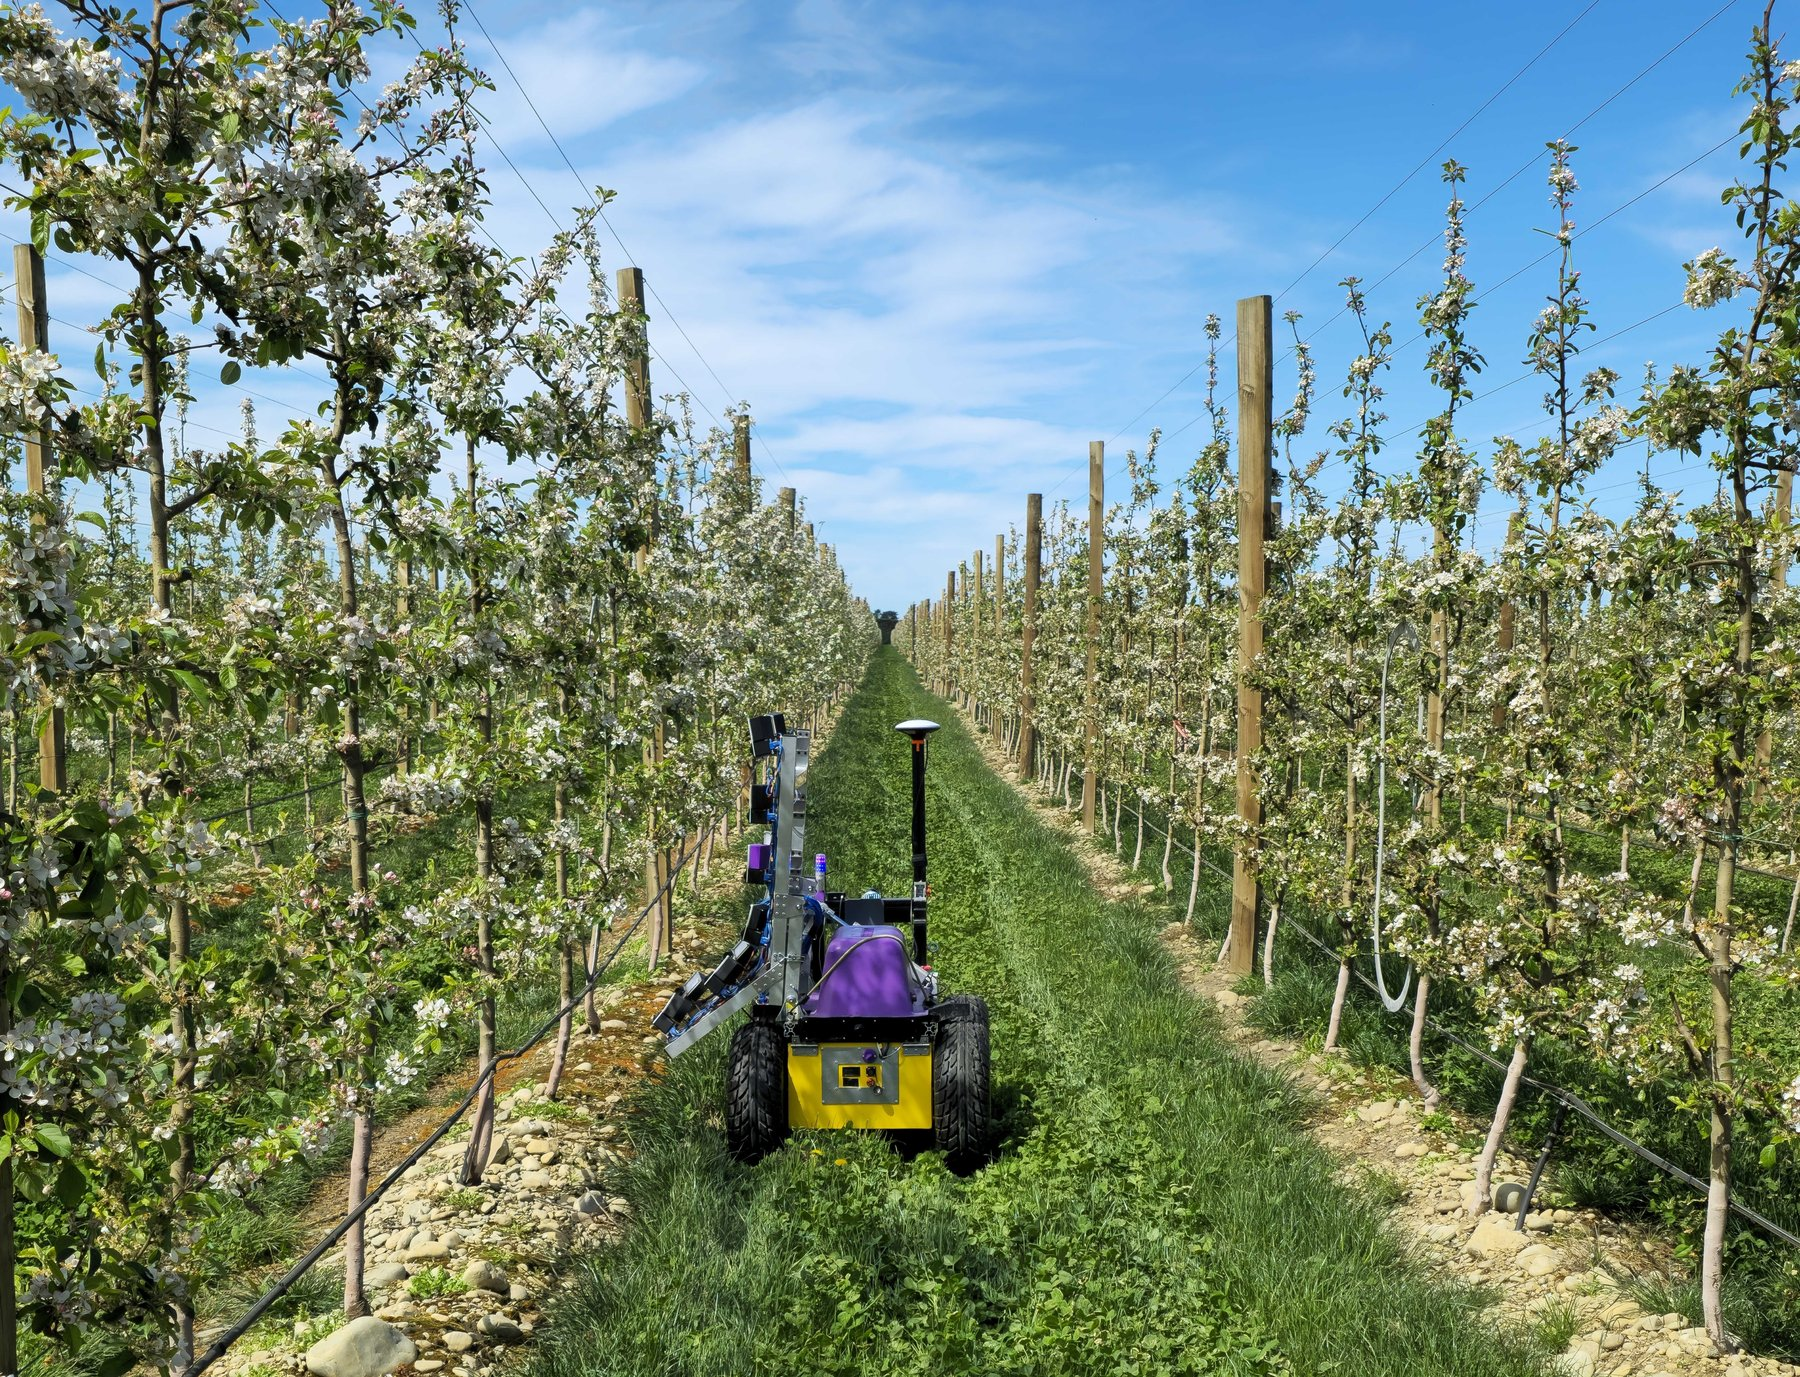
\includegraphics[width=0.85\linewidth]{1-intro/figures/robot_in_apple_orchard.jpg}
    \caption{The UCVision rover navigating an apple orchard row during a data-collection pass. The platform captures multi-view imagery used to generate offline 3D reconstructions for yield prediction and precision agricultural tasks.}
    \label{fig:robot-apple-orchard}
\end{figure}

\section{Research Context}
\label{sec:research-context}

This thesis is situated within the broader research initiatives of the University of Canterbury Computer Vision Research Group (UCVision), specifically contributing to the MBIE funded project, `Predicting the unseen: a new method for accurate yield estimation in viticulture/horticulture'. This project utilises autonomous field robots (\cref{fig:robot-apple-orchard}) to capture multi-view imagery of vineyards and orchards, which are subsequently processed \textit{offline} to generate high-fidelity 3D reconstructions using 3D Gaussian Splatting (3DGS). These models serve as the ``digital twin'' required for complex agricultural tasks such as precision yield estimation and autonomous intervention.

The primary objective of this project is the automation of vineyard pruning. In this workflow, pruning decisions and robotic arm path planning are computed within the high-fidelity 3DGS environment. Unlike conventional pruning systems that rely on lower-resolution, real-time sensor data for immediate modelling and execution, the UCVision workflow decouples data collection from intervention. While this allows for superior structural analysis of the vine, it introduces a fundamental spatial synchronisation problem: the alignment of the robot's current pose to the offline model's coordinate frame.

For the robot to execute a pre-computed pruning plan, it must map its real-time physical state to the coordinate system of the offline model. This necessitates a robust SLAM framework capable of solving three distinct sub-problems:
\begin{enumerate}
    \item \textbf{Global Relocalisation:} Navigating the platform back to the specific plant or row identified in the modelling phase.
    \item \textbf{Strategic Positioning:} Aligning the mobile base within the physical workspace constraints of the robotic arm to ensure all required cutpoints are reachable.
    \item \textbf{Sim-to-Real Registration:} Achieving centimetre-level alignment between the robot's onboard perception and the 3D model, ensuring that the path planner's simulated coordinates correspond precisely to the physical vine structures.
\end{enumerate}

To the author's knowledge, no existing vineyard robotics system addresses this full registration chain. Current pruning platforms assume a tightly coupled perception--execution loop in which the model is built and consumed in real time; they do not face the problem of aligning a robot to a pre-built offline reconstruction. Similarly, existing agricultural SLAM systems target navigation-grade accuracy and do not provide the centimetre-level pose refinement required for manipulation against an offline model.

This thesis addresses this capability gap by developing a SLAM and relocalisation framework that enables the registration chain described above. By synchronising the robot’s perceived position with both the physical environment and the pre-existing 3D model, this research enables the transition from static digital twins to active, autonomous robotic intervention in the field.
\section{Research Motivation}
\label{sec:motivation}

This research is primarily motivated by the need to enable autonomous agricultural robots to perform complex manipulation tasks, specifically robotic pruning. Unlike simple navigation, pruning requires a high-fidelity Simultaneous Localisation and Mapping (SLAM) framework that can provide the centimetre-level precision necessary for a robotic arm to interact with thin, overlapping vine structures. This tolerance is derived from the physical geometry of the pruning tool: pruning secateurs have a jaw opening of approximately 25--30\,mm, while dormant canes targeted for removal are typically 10--15\,mm in diameter~\cite{pennstateextensionDormantCaneSpur2023}, leaving roughly 10\,mm of clearance per side within which localisation error can be absorbed. Maintaining such accuracy in the presence of dynamic foliage and repetitive, unstructured row patterns remains a critical bottleneck in automating viticulture and horticulture.

The demand for such technology is underscored by the economic landscape of New Zealand's primary industries. As of 2026, horticulture export revenue is forecast to reach a record NZ\$9.2 billion, with wine production constituting NZ\$2.3 billion~\cite{industriesSituationOutlookPrimary2025}. However, the sector faces chronic labour shortages and rising operational costs, with manual pruning alone accounting for approximately 21\% of annual vineyard expenses~\cite{industriesMarlboroughVineyardMonitoring2025}.

The 2025 Vineyard Monitoring Report published by the Ministry for Primary Industries indicates that during the 2024/2025 season, expenditure on manual pruning increased, while spending on machine pruning declined by 21\%. This shift is attributed to grower concerns regarding vine damage caused by current mechanical stripping machines~\cite{industriesMarlboroughVineyardMonitoring2025}. These concerns highlight the principal limitation of current commercial machine-based pruning systems: the inability to selectively remove individual canes without compromising cordon or trunk wood. Overcoming these precision challenges would enable robotic automation to provide a scalable response to ongoing workforce constraints, thereby supporting the long-term sustainability of New Zealand’s high-value horticultural crops.

Beyond the immediate application to pruning, this work also contributes to UCVision's broader mission of modelling occluded plant structures and tracking growth across multiple seasons.





\section{Research Objectives}
\label{sec:research-objectives}

The primary objective of this research is to develop a precise localisation system for autonomous vineyard robots that enables accurate spatial alignment between the robot, the 3D models, and the environment.

The research pursues the following sub-objectives:

\begin{enumerate}

    \item Develop a LiDAR-inertial SLAM system that achieves sub-decimetre absolute trajectory error in GNSS-degraded vineyard environments, addressing the structural ambiguity of row-crop corridors.

    \item Design a precise-alignment pipeline that refines the SLAM pose to sub-centimetre accuracy by registering live sensor data against a 3D Gaussian Splatting reference model using point cloud registration.

    \item Evaluate two sensing modalities (stereo vision and LiDAR) for the precise-alignment stage, comparing their registration accuracy and failure modes under vineyard field conditions.

    \item Integrate both localisation stages into a hierarchical architecture that provides pose estimates suitable for downstream robotic manipulation, such that the corrected pose feeds directly into the pruning arm's path planner.

\end{enumerate}

\subsection{Contributions}
\label{subsec:contributions}

This thesis makes the following contributions:

\begin{enumerate}
    \item A LiDAR-inertial SLAM system augmented with sparse GNSS factor injection (GLIM-GNSS) that achieves 71--174\,mm absolute trajectory error across five vineyard datasets while utilising less than 1\% of available GNSS measurements, demonstrating that sub-decimetre localisation is attainable in repetitive row-crop environments without continuous RTK coverage.

    \item A precise-alignment pipeline that registers live point cloud data against a pre-built 3D Gaussian Splatting reference model via Generalised Iterative Closest Point, achieving centimetre-scale pose refinement (15.51\,mm mean inlier RMSE for stereo; 33.25\,mm median inlier RMSE for LiDAR) from a coarse SLAM initialisation.

    \item A comparative evaluation of LiDAR and stereo vision modalities for vine-scale registration, characterising their convergence--accuracy trade-off: LiDAR achieves 100\% condition-level convergence while stereo produces lower RMSE (78\% convergence), with both modalities confirming that the SLAM-derived pose lies within the registration algorithm's convergence basin.
\end{enumerate}
\section{Thesis Structure}
\label{sec:thesis-structure}

This thesis is structured as follows:
\Cref{chap:Background} establishes the theoretical and practical foundations of robot localisation for vineyard manipulation tasks, reviewing probabilistic estimation, point cloud registration, and domain-specific SLAM approaches.
\Cref{chap:SLAM} presents the development and evaluation of a multi-sensor SLAM system for initial mapping and coarse localisation within vineyard environments. 
\Cref{chap:precise-alignment} describes the precise-alignment methodology, wherein robot pose estimates are refined through registration with pre-existing 3D models using stereo depth imaging, dense LiDAR, and Iterative Closest Point (ICP) algorithms. 
\Cref{chap:Conclusion} concludes with a synthesis of key findings and recommendations for future research.



\chapter{Background}
\label{chap:Background}

\section{Robot Localisation}
\label{sec:robot-localisation}

Robot localisation is the process of estimating a robot's pose (position and orientation) within a given reference frame using sensory information. It is a prerequisite for all navigation and manipulation tasks that require interaction with the physical environment, and is tightly coupled with mapping; together they constitute Simultaneous Localisation and Mapping (SLAM)~\cite{ullahMobileRobotLocalization2024,leonardSimultaneousMapBuilding1991}.

This section traces the historical foundations of robot localisation, structured around three persistent challenges that have shaped the field and that remain directly relevant to the methods presented in this thesis. The first is the accumulation of pose error under dead reckoning, which motivates a probabilistic treatment of uncertainty. The second is the need to represent and fuse uncertain, heterogeneous sensor measurements into a coherent spatial model. The third is the tension between short-range alignment and global map consistency. The foundational contributions reviewed here (probabilistic uncertainty modelling~\cite{smithRepresentationEstimationSpatial1987}, occupancy-based sensor fusion~\cite{elfesUsingOccupancyGrids1989}, the Iterative Closest Point (ICP) algorithm~\cite{beslMethodRegistration3D1992a}, and pose graph optimisation~\cite{luGloballyConsistentRange1997}) constitute the algorithmic backbone of the SLAM system developed in \cref{chap:SLAM} and the precise-alignment pipeline described in \cref{chap:precise-alignment}.

\subsection{The Limits of Deterministic Localisation}
\label{subsec:deterministic-localisation}

The first mobile robots capable of autonomous reasoning operated under deterministic models: each commanded action was assumed to execute perfectly, and the robot's pose was updated accordingly. Shakey the Robot (1966--1972) localised through discrete semantic labels and open-loop dead reckoning, with landmark correction that depended on the environment conforming exactly to a pre-modelled structure~\cite{nilssonShakeyRobot1984}. Moravec's Stanford Cart extended this to geometric localisation via stereo vision, maintaining explicit 3D feature positions but associating no uncertainty with them; errors accumulated silently, requiring approximately five hours for a 20-metre indoor traverse~\cite{moravecObstacleAvoidanceNavigatio1980,moravecStanfordCartCMU1990}.

These systems illustrate the core failure mode of deterministic localisation: uncorrected motion errors compound over time, and landmark-based correction is unreliable whenever the observed environment departs from assumed models. In semi-structured outdoor environments such as vineyards, where plant geometry changes seasonally, features repeat along rows, and no guaranteed prior map exists, this fragility is not a boundary case but the normal operating condition. The response was to replace deterministic pose estimates with probabilistic representations that could explicitly track and propagate uncertainty.

\subsection{Uncertainty Representation and Sensor Fusion}
\label{subsec:uncertainty-sensor-fusion}

The shift to probabilistic localisation was formalised by Smith and Cheeseman~\cite{smithRepresentationEstimationSpatial1987}, who proposed representing each spatial relationship as an \textit{approximate transformation}: a pose estimate paired with a covariance matrix encoding second-order uncertainty. Their framework introduces two fundamental operations. \textit{Compounding} propagates uncertainty through sequential transformations: when two uncertain poses are composed, the resulting covariance grows as a function of both input uncertainties, formalising what Shakey and the Cart demonstrated empirically: drift accumulates with each successive motion. \textit{Merging} reduces uncertainty by fusing independent estimates of the same quantity via a minimum-variance weighted combination, yielding a posterior covariance smaller than either input.

In a subsequent paper, Smith, Self, and Cheeseman extended this framework to the Stochastic Map~\cite{smithEstimatingUncertainSpatial2013}, in which robot and landmark poses are jointly maintained in a single state vector, the formulation underpinning Extended Kalman Filter (EKF) SLAM.

Building on this probabilistic foundation, Elfes introduced occupancy grids~\cite{elfesUsingOccupancyGrids1989}: a spatial representation in which each cell of a tessellated lattice maintains a probabilistic occupancy estimate, updated incrementally from raw sensor data through an explicit sensor model. A key insight is that individual sensor modalities carry complementary uncertainty profiles: sonar provides low range uncertainty but poor angular resolution, while stereo cameras offer good angular resolution but depth uncertainty that grows with distance. Representing both in a common occupancy-grid format allows them to be fused into a map with lower aggregate uncertainty than either source alone, as illustrated in \cref{fig:occupancyGridSensorFusion}.

Elfes also noted that fusing sensor views into a coherent global map requires accurate motion estimation, since dead-reckoning uncertainty compounds in precisely the manner formalised by Smith and Cheeseman. This co-dependence between localisation accuracy and map quality is the defining characteristic of SLAM, and directly motivates the choice in \cref{chap:SLAM} to fuse LiDAR odometry with an inertial measurement unit (IMU) whose complementary error characteristics reduce drift under the same merging principle.

\begin{figure}
    \centering
    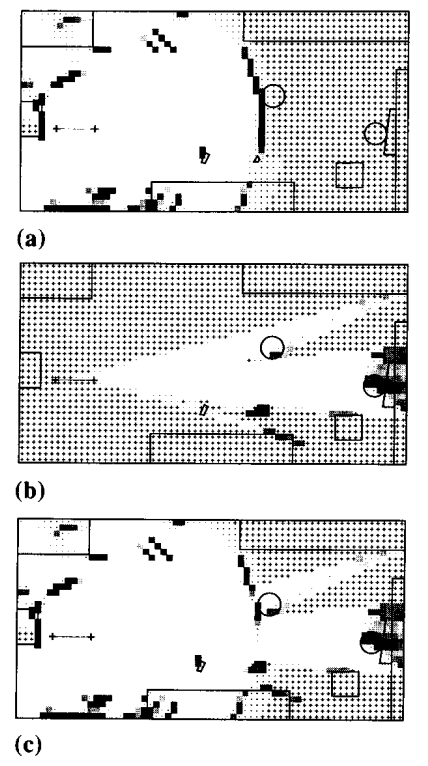
\includegraphics[width=0.5\linewidth]{2-background/figures/OccupancyGridSensorFusion.png}
    \caption{Sensor integration of sonar and scanline stereo. Occupancy grids generated separately for sonar (a) and scanline stereo (b), as well as the integrated map (c) obtained through sensor fusion, are shown. Occupied regions are marked by shaded squares, empty areas by dots fading to white space, and unknown spaces by + marks \protect\cite{elfesUsingOccupancyGrids1989}. }
    \label{fig:occupancyGridSensorFusion}
\end{figure}

\subsection{Point Cloud Registration}
\label{subsec:point-cloud-registration}

Relative pose estimation between sensor frames requires a method for aligning observations acquired at successive robot positions. Besl and McKay's Iterative Closest Point (ICP) algorithm~\cite{beslMethodRegistration3D1992a} frames registration as an optimisation problem: starting from an initial alignment, it alternates between assigning each source point to its nearest neighbour in the target cloud and solving for the rigid transformation that minimises the mean squared distance over all correspondences. Monotonic convergence of the cost function is guaranteed; however, the solution is sensitive to initial conditions and requires sufficient geometric overlap between the two clouds. Subsequent variants, notably point-to-plane error metrics~\cite{chenObjectModelingRegistration1991} and the probabilistic Generalised-ICP formulation~\cite{segalGeneralizedICP2009}, improved convergence speed and robustness in environments lacking strong planar structure.

ICP is the direct registration engine used in the precise-alignment pipeline described in \cref{chap:precise-alignment}, where a real-time point cloud of a physical vine is aligned against the SfM-derived reference geometry extracted from a 3D Gaussian Splatting model. The sensitivity of ICP to initialisation and partial overlap is a central practical constraint addressed in that chapter.

\subsection{Pose Graph Optimisation and Global Consistency}
\label{subsec:pose-graph-optimisation}

Probabilistic uncertainty modelling and local scan matching together support accurate short-range pose estimation, but do not address a deeper limitation: errors accumulated along a long trajectory cannot be corrected retroactively by filtering methods. EKF-based SLAM incorporates past measurements into a sufficient statistic and then discards the raw observations; over extended trajectories, linearisation errors accumulate and the filter becomes internally inconsistent, with different regions of the map updated independently and unable to be reconciled.

Lu and Milios addressed this by introducing pose graph optimisation~\cite{luGloballyConsistentRange1997}. In a pose graph, each estimated robot pose is a node, and each relative spatial constraint (derived from scan matching or odometry) is an edge. The optimisation objective is to find the configuration of all nodes that best satisfies the full set of edge constraints simultaneously. Because the entire history of pose estimates is retained, a single loop-closure detection event can propagate corrections backward through the trajectory, recovering a globally consistent map. The fundamental contrast with filtering is that past states are not discarded: global consistency is achieved through a batch optimisation rather than a recursive update, at the cost of a more demanding solve.

For long traversals through vineyard rows, where cumulative drift along the row axis would otherwise render multi-row maps geometrically inconsistent, this distinction is operative. The SLAM system presented in \cref{chap:SLAM} employs pose graph optimisation as its back-end, enabling loop-closure corrections to enforce global consistency across traversals of multiple vineyard rows.

\subsection{Summary}
\label{subsec:robot-localisation-summary}

The foundational methods reviewed in this section address three persistent challenges that remain operative in the vineyard localisation problem addressed by this thesis. First, pose error accumulates under dead reckoning and must be explicitly modelled and propagated, demanding a probabilistic treatment of estimation. Second, no single sensor is sufficient for robust localisation; each modality carries characteristic errors, and heterogeneous sensor fusion governed by the merging operations formalised by Smith and Cheeseman is necessary to reduce aggregate uncertainty. Third, local consistency from scan matching and global consistency from loop-closure correction are distinct requirements, and satisfying both simultaneously requires a graph-based optimisation back-end. The systems developed in \cref{chap:SLAM} and \cref{chap:precise-alignment} address these three challenges in sequence. The following section examines how these challenges manifest within vineyard and orchard environments, where domain-specific constraints have motivated a distinct body of applied SLAM research.



\section{Robot Localisation in Vineyard and Orchard Robotics}

Unlike structured industrial settings, agricultural environments are "semi-structured" environments characterised by homogeneous structures, seasonal variability, and dynamic occlusion \cite{hroobBenchmarkVisual3D2021}. Moreover, the reliance on Global Navigation Satellite Systems (GNSS) often falls short in orchards as dense canopies can attenuate satellite signals or induce multipath errors, making standard GNSS insufficient for centimetre-level precision tasks \cite{tangFruitTreeMappingSystem2024}. Therefore, research has focused on developing technologies that use semantic understanding, geometric constraints, and multi-sensor fusion to operate reliably in these GNSS-denied environments \cite{tangFruitTreeMappingSystem2024}.

\subsection{Environmental Constraints and Challenges}
Semi-structured agricultural environments create unique constraints that pose a challenge for generic SLAM algorithms designed for structured urban environments. 

\paragraph{Perceptual Aliasing and Geometric Repetitiveness}

Commercial crops in vineyards and orchards are planted in long, parallel rows with uniform spacing to maximise yield and facilitate machine access. The long uniform rows create a ``corridor effect'', especially for LiDAR-based systems. The corridor effect is characterised by the absence of distinct geometric features along the longitudinal position of the robot (the direction of movement down the row), such that the longitudinal axis becomes unobservable, which can lead to significant drift in the estimated trajectory as the robot cannot determine if it has travelled one metre forward or five metres forward \cite{khanReviewSLAMTechniques2025}. Visual systems face a similar challenge wherein standard feature descriptors (e.g., ORB, SIFT) extracted from one part of a row are statistically indistinguishable from those in another, resulting in erroneous feature matching and false-positive loop closure \cite{papadimitriouLoopClosureDetection2022}.

\paragraph{Dynamic and Unstructured Environment}
Many SLAM systems make an assumption of a static world, however orchards and vineyards are dynamic environments. Short-term dynamics such as wind-induced canopy motion, workers, and machines can pose challenges to mapping and loop closure. Long-term dynamics include seasonal changes, wherein a map constructed during the dormant winter season can differ greatly compared with the full-canopy summer season. This can pose challenges to long-term localisation and map maintenance \cite{schmidtROVERMultiSeasonDataset2024}.

Furthermore, the uneven terrain can cause camera shake and wheel slippage that introduces high-frequency noise into odometry estimates \cite{zhangKeyTechnologiesIntelligent2026}.

\subsection{LiDAR SLAM}

LiDAR SLAM is often favoured due to its illumination invariance, but standard scan-matching algorithms like ICP often fail in symmetric vineyard rows due to the aforementioned perceptual aliasing along the longitudinal axis. 

VineSLAM tries to address the perceptual aliasing problem by grouping point clouds into specific vineyard features: semi-planes (for the continuous canopy/trellis) and points (for trunks/posts). It utilises a Particle Filter that fuses these features; semi-planes offer lateral constraints to keep the robot centred, and point features provide longitudinal constraints along the row. Comparative studies show VineSLAM outperforms general-purpose algorithms like LeGO-LOAM in symmetric corridors \cite{aguiarLocalizationMappingAgriculture2022}.

Tree-SLAM detects individual tree trunks within the point clouds, mapping the environment as a sparse graph of tree landmarks rather than a dense point cloud. This method achieved localisation errors as low as 18 cm for individual trees (less than 20\% of standard planting distance) in apple and pear orchards \cite{rapado-rinconTreeSLAMSemanticObject2025a}. This object-level approach improves navigation but also facilitates agronomic tasks such as per-tree yield monitoring \cite{rapado-rinconTreeSLAMSemanticObject2025a}. 

The April-LIO-SAM framework tightly couples LiDAR-Inertial Odometry (LIO-SAM) with AprilTags acting as artificial landmarks. April tags provide absolute pose constraints that constrain the drift from LiDAR odometry. Experimental validation in orchards demonstrated that with tags spaced at 3 to 5 metres, the system achieves a root-mean-square error (RMSE) of approximately 0.057 m, maintaining stability even under occlusion and varying illumination \cite{guanResearchAgriculturalAutonomous2025}. Another multi-sensor system achieved positioning errors of 0.57 cm in pear orchards, using visual data for loop closure and LiDAR for geometric structure \cite{tangFruitTreeMappingSystem2024}.

\paragraph{Benchmarking Datasets}
Progress in the field is accelerated by open-source datasets tailored to agricultural challenges:
\begin{itemize}
    \item \textbf{MAgro Dataset:} Collected in apple and pear orchards using LiDAR, stereo cameras, and RTK-GPS. It is designed to benchmark loop closure and localisation under varying weather and illumination conditions \cite{schmidtROVERMultiSeasonDataset2024} \cite{marzoatancoMAgroDatasetDataset2024}.
    \item \textbf{Bacchus Long-Term (BLT) Dataset:} A unique dataset capturing a vineyard over a 7-month period. It supports research into "lifelong SLAM," challenging algorithms to handle the drastic morphological changes of the canopy from winter dormancy to summer harvest \cite{polvaraBacchusLongTermBLT2024}.
    \item \textbf{AgriLiRa4D:} A recent multi-modal dataset (LiDAR, Camera, 4D Radar) collected via UAV over diverse terrains (flat, hilly), facilitating research into radar-based fusion and aerial coverage paths \cite{zhanAgriLiRa4DMultiSensorUAV2026}.
\end{itemize}

\subsection{Conclusion}
The development of SLAM for orchards and vineyards has evolved from the application of generic algorithms to the design of domain-specific architectures. Current research prioritises semantic SLAM to filter dynamic agricultural noise and object-level mapping (e.g., Tree-SLAM) to resolve geometric ambiguity. Furthermore, the integration of multi-sensor fusion (e.g., April-LIO-SAM) has proven essential for achieving the centimetre-level accuracy required for precision tasks. Future work is increasingly driven by long-term autonomy, leveraging datasets like BLT to enable robots that can adapt to the seasonal biological evolution of the crop \cite{tangFruitTreeMappingSystem2024} \cite{polvaraBacchusLongTermBLT2024}.

\section{Robot Localisation in Vineyard Pruning}
\label{sec:vineyard-pruning}
Pruning typically occurs in the dormant season (winter), which introduces a unique robot localisation challenge in the form of geometric sparsity and the lack of distinctive visual features caused by the absence of foliage~\cite{youOpticalFlowbasedBranch2022}. The environment consists of thin, bare branches that provide a low density of sensor returns and few distinctive visual textures for cameras to localise on~\cite{youOpticalFlowbasedBranch2022}. Without leaves to block the view, sensors often pick up background clutter from the sky or neighbouring rows, complicating foreground segmentation~\cite{youOpticalFlowbasedBranch2022}. The following analysis details the strategies used for spatial alignment with vines, specifically in the context of robotic pruning platforms.

\subsection{Spatial Alignment Modalities for Pruning Vines}
\label{subsec:spatial-alignment-modalities}
While traditional passive vision remains the baseline for high-resolution 3D modelling, it faces significant geometric and environmental hurdles. To address the ill-conditioned configurations of binocular systems, specifically when linear canes align with the stereo baseline, Botterill et al. employ a trinocular rig consisting of three 1.3-megapixel cameras arranged in a triangular configuration, housed within a vine-straddling mobile platform (\cref{fig:botterilRobot})~\cite{botterillRobotSystemPruning2017}. This allows for the dynamic selection of the mathematically optimal camera pair for specific cane segments, a level of geometric robustness that passive binocular systems lack.

\begin{figure}[ht]
    \centering
    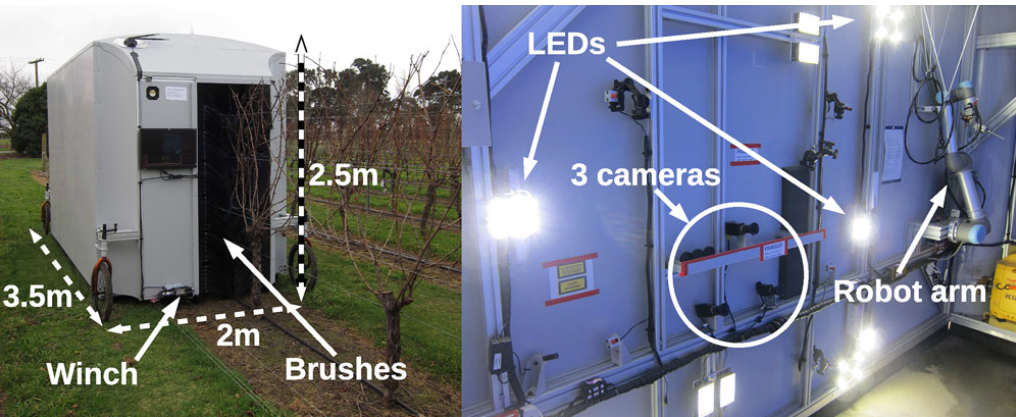
\includegraphics[width=0.85\linewidth]{2-background/figures/botterilRobot.png}
    \caption{The vine-straddling mobile platform developed by Botterill et al., shown from outside (left) and inside (right). The enclosed structure shields the workspace from ambient sunlight, while the interior houses the trinocular camera array, high-intensity LED illumination, a six degree-of-freedom robot arm, and an on-board PC for real-time processing \protect\cite{botterillRobotSystemPruning2017}.}
    \label{fig:botterilRobot}
\end{figure}

However, even optimised trinocular systems remain vulnerable to outdoor lighting variability. This necessitates a shift toward active sensing, either through illumination or direct range-finding. The Bumblebee platform integrates an active light stereo camera system to generate dual point clouds, which are registered via transformation matrices and refined with the Iterative Closest Point (ICP) algorithm to maintain invariance against ambient shadows~\cite{silwalBumblebeePath2022}. Active-light camera designs of this type also improve robustness to varying outdoor illumination more broadly~\cite{silwalRobustIlluminationInvariantCamera2021}. In contrast, Felicetti et al. bypass the lighting and correspondence problem entirely by utilising downward-facing 3D LiDAR~\cite{felicettiTractorMountedGrapevine2025}. By applying a minimalist depth-thresholding algorithm within a specific range ($D_{min}$ to $D_{max}$, typically 250--500 mm), this approach sacrifices the fine-grained topological understanding provided by Botterill's trinocular rig in favour of throughput, processing a vine in just 7.3 seconds~\cite{felicettiTractorMountedGrapevine2025, botterillRobotSystemPruning2017}.

The data processing pipelines of these approaches are also vastly different. Botterill et al. prioritise spatial stability for robotic manipulation through a heavy incremental bundle adjustment pipeline. By utilising the \textit{g2o} graph optimisation framework and robust Pseudo-Huber cost functions to penalise large residuals, they achieve trajectory errors below 1\%, though at a higher computational cost~\cite{botterillRobotSystemPruning2017}. Recent work, however, suggests that such global optimisation may be unnecessary for effective pruning. The Archie Jnr platform employs deep panoptic segmentation (Detectron2) to identify cane structures and nodes, enabling autonomous vine assessment for three-cane pruning decisions~\cite{williamsArchieJnrRobotic2024}. Separately, Hizatate et al. propose a system combining RGB-D cameras with a 6-DoF manipulator, estimating grapevine structures to identify pruning points with 62\% accuracy~\cite{hizatateDevelopmentRobotPruning2025}.

By registering segmentation masks with depth data, these neural architectures occupy the middle ground between the high-fidelity reconstruction of Botterill et al. and the high-speed approach of Felicetti et al. Williams et al. demonstrate that Archie Jnr successfully prunes 71.1\% of required canes across real-world vineyard trials~\cite{williamsArchieJnrRobotic2024}, while Bumblebee's active lighting and Faster R-CNN bud detection pipeline provides the precision required for dormant-season cane identification~\cite{silwalBumblebeePath2022}. The trinocular approach provides the most detailed 3D map for precise spur pruning, but the integration of active illumination and semantic segmentation offers a more computationally viable path toward commercial field speeds.

\begin{table}[h]
\centering
\caption{Comparison of Perception Modalities for Vineyard Pruning}
\label{tab:perception}
\begin{tabularx}{\textwidth}{|X|l|l|}
\hline
\textbf{System} & \textbf{Modality} & \textbf{Key Metric} \\ \hline
Botterill et al.~\cite{botterillRobotSystemPruning2017} & Trinocular Stereo & 120 s/vine \\ \hline
Bumblebee~\cite{silwalBumblebeePath2022} & Active Light Stereo & 137 s/vine \\ \hline
Felicetti et al.~\cite{felicettiTractorMountedGrapevine2025} & 3D LiDAR & 7.3 s/vine \\ \hline
Archie Jnr~\cite{williamsArchieJnrRobotic2024} & RGB-D + Panoptic Seg. & 71.1\% prune success \\ \hline
Hizatate et al.~\cite{hizatateDevelopmentRobotPruning2025} & RGB-D + 6-DoF Arm & 62\% accuracy \\ \hline
\end{tabularx}
\end{table}

\subsection{Summary}
\label{subsec:vineyard-pruning-summary}

Existing robotic pruning platforms demonstrate that millimetre-level spatial alignment is achievable, but they share a common architectural assumption: perception, planning, and execution are tightly coupled within a single real-time pipeline. The UCVision approach departs from this assumption by decoupling the data-collection phase from the intervention phase, generating a high-fidelity 3D Gaussian Splatting model offline before any manipulation is attempted. This decoupling introduces a spatial synchronisation problem that no existing pruning platform directly addresses: given a pre-computed pruning plan expressed in the coordinate frame of an offline 3D model, how can a robot executing that plan achieve the centimetre-level registration accuracy necessary to transfer planned cut-points to physical vine structures? This gap motivates the contributions of \cref{chap:SLAM} and \cref{chap:precise-alignment}.





\chapter{SLAM}
\label{chap:SLAM}

\section{Introduction}
\label{sec:slam-intro}
This chapter presents the development and evaluation of a LiDAR-inertial SLAM pipeline designed to operate independently of frequent GNSS updates, targeting three core requirements. First, the system must achieve high-fidelity localisation in GNSS-denied or GNSS-degraded scenarios. Second, the SLAM front-end must remain invariant to fluctuating visual appearances, enabling continuous operation across diurnal cycles, varying weather conditions, and seasonal plant growth. Third, as described in \cref{chap:Background}, vineyard and orchard rows form long, symmetric, corridor-like structures that limit the geometric diversity available to scan-matching algorithms, making them susceptible to ambiguity and longitudinal drift, as illustrated in \cref{fig:slam-map-zoomed-out}. The system presented in this chapter is therefore not intended as a general-purpose SLAM solution; it is a specialised architecture targeted at the structural and perceptual characteristics of row-crop environments such as vineyards and orchards. The two primary contributions of this chapter are: (i) a systematic hyperparameter optimisation methodology for tuning LiDAR-inertial SLAM to the specific geometric and operational demands of row-crop environments, and (ii) an extension of the SLAM back-end to incorporate sparse GNSS factors, enabling bounded long-term drift without continuous RTK availability.

\begin{figure}[htbp]
    \centering
    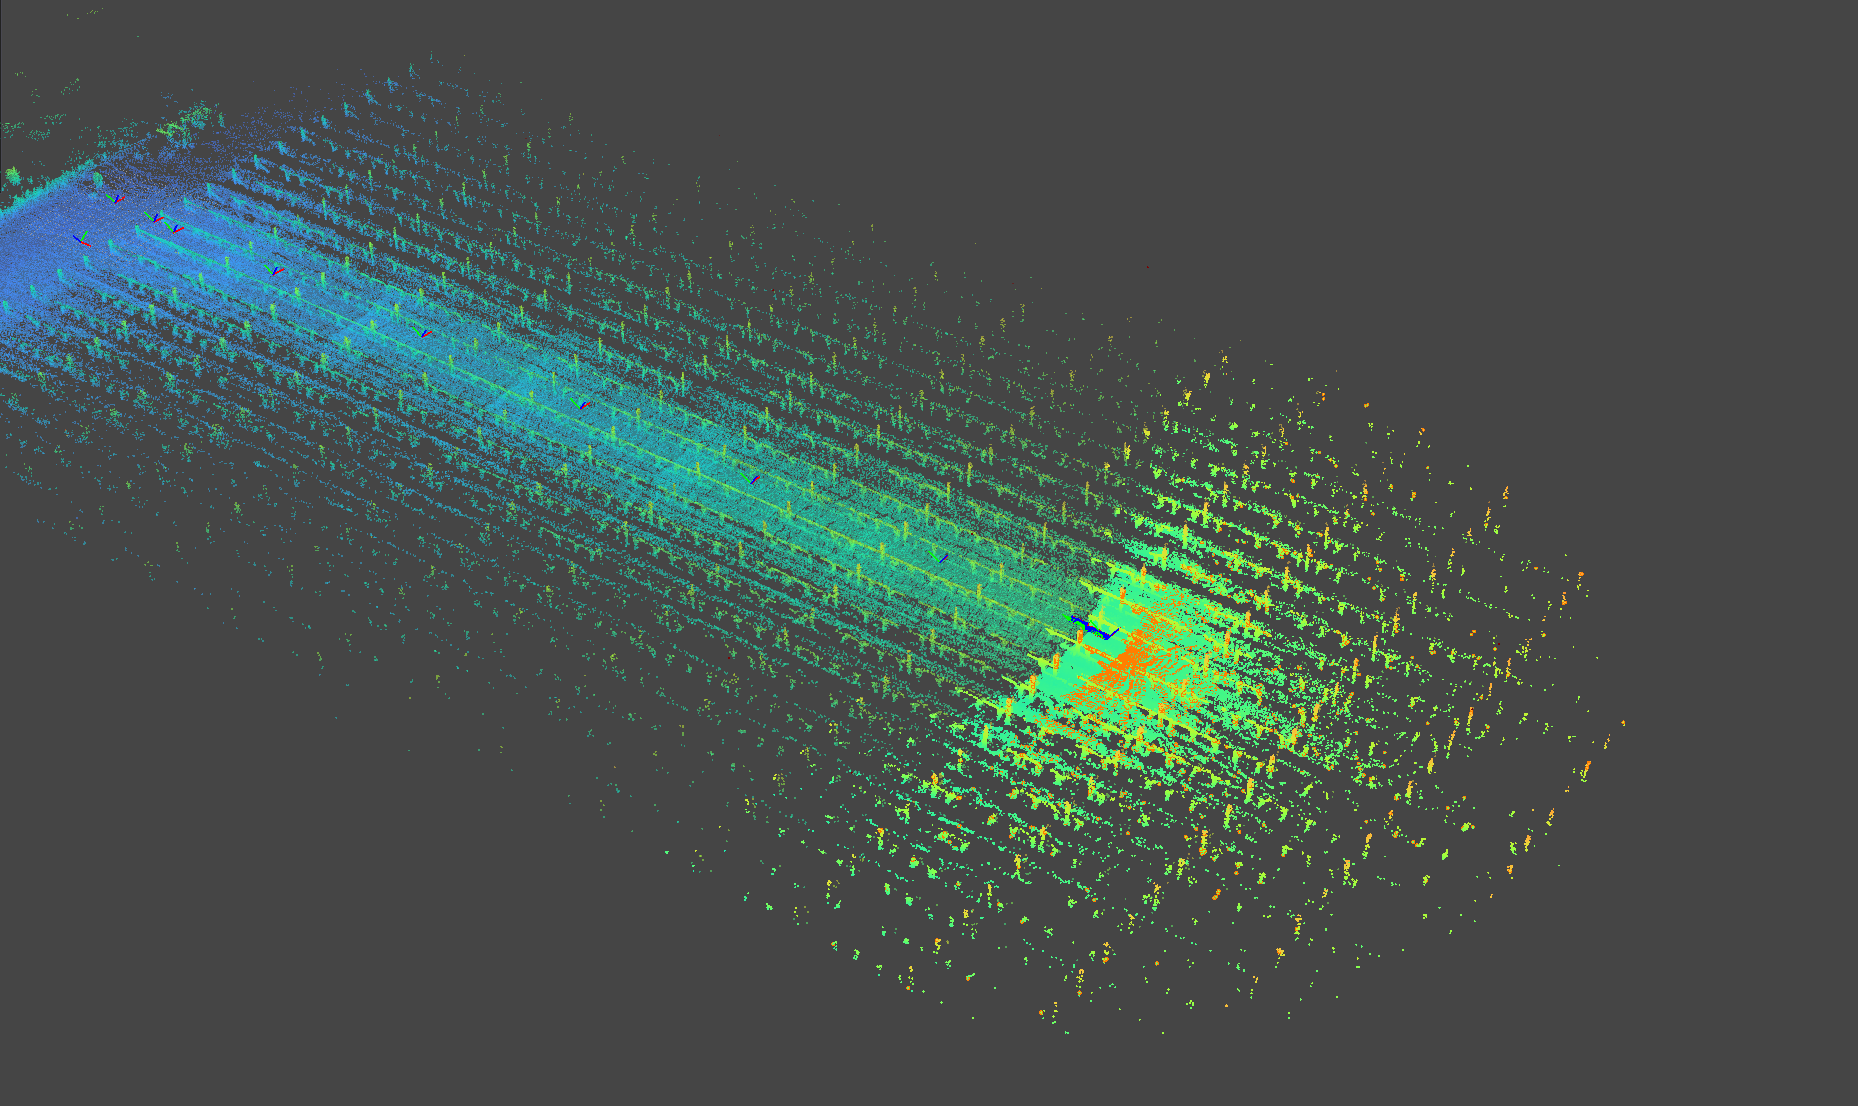
\includegraphics[width=0.85\linewidth]{3-SLAM/3-intro/figures/slam_map_zoomed_out.png}
    \caption{LiDAR point cloud accumulated mid-traversal by the GLIM-GNSS system in the UCVision vineyard (height-coded colouring). The robot is still progressing down a row; the rightmost region of the map remains unvisited.}
    \label{fig:slam-map-zoomed-out}
\end{figure}

\subsection{Motivation}
\label{subsec:slam-motivation}
The necessity for this research stems from the operational limitations of the current UCVision Rover localisation system. Prior iterations of this platform utilised an Extended Kalman Filter (EKF) heavily reliant on Real-Time Kinematic (RTK) GPS data. While precise under open skies, this dependency proved non-viable for robust field operations where tree canopies, topography, and public RTK base station blackouts frequently cause signal multipath or dropout. Adverse weather further compounds this unreliability: heavy precipitation increases tropospheric delay errors \cite{solheimPropagationDelaysGPSSignals1999} and multipath reflections from wet vegetation \cite{nievinskiForwardModelingGPSMultipath2014}, while ionospheric disturbances — which are more frequent during solar weather events and magnetic storms — introduce rapid carrier-phase cycle slips that break the integer ambiguity fix and degrade the RTK solution from centimetre-level fixed accuracy to decimetre-level float accuracy or worse \cite{wielgoszAnalysisNetworkRTKIonospheric2005}. In practice, a significant proportion of field scans conducted with the UCVision Rover were rendered unusable due to the inability to acquire or sustain a consistent RTK fix, causing the localisation system to fail entirely.

Transitioning to a LiDAR-centric SLAM approach, tailored to these agricultural environments, provides three distinct advantages:
\begin{itemize}
	\item \textbf{Reduced GNSS dependence:} By shifting the primary motion estimation to scan-matching and loop closure, the system operates with sub-1\% GNSS factor utilisation, removing the requirement for continuous RTK availability.
	\item \textbf{Corridor robustness:} The architecture presented here specifically addresses the structural challenges of row-crop environments through vineyard-focused parameterisation and sensor fusion suited to row-structured terrain.
	\item \textbf{Downstream utility (design intent):} Beyond localisation, the high-density LiDAR maps generated provide a foundation for additional tasks such as landmark detection (e.g., vine trunks and trellis posts), spatial alignment of Gaussian splats captured from opposing sides of a row, and global registration of data across multiple vineyard bays. These downstream applications are not evaluated in this chapter but motivate the map quality requirements.
\end{itemize}

\clearpage

\section{Related Work}
\label{sec:slam-related-work}
The development of Simultaneous Localisation and Mapping (SLAM) has shifted from laboratory settings to complex, real-world deployments across autonomous driving, aerial vehicles, and subterranean exploration. Due to the limitations of external positioning systems such as GNSS in dynamic or urban environments, Light Detection and Ranging (LiDAR) has become the dominant sensing modality, providing high-fidelity, active 3D geometry independent of ambient illumination. The state of the art in this field is defined by LiDAR-Inertial Odometry (LIO), which tightly couples LiDAR measurements with high-frequency inertial data from an Inertial Measurement Unit (IMU) to compensate for motion distortion and maintain observability in geometrically degenerate scenes \cite{koideGLIM3DRangeInertial2024}. Modern LIO research is primarily distinguished by a bifurcation of techniques into two dominant optimisation philosophies: Error-State Kalman Filtering (ESKF) and Factor Graph Optimisation (FGO). This review traces the architectural evolution of LIO, comparing and contrasting leading algorithms such as LIO-SAM, FAST-LIO2, GLIM, and Super-LIO to synthesise the current trends in computational efficiency and global consistency.

\subsection{Modern LiDAR-SLAM Architectures}
\label{subsec:lidar-slam-architectures}
The foundation of modern LiDAR SLAM rests on the seminal LOAM (LiDAR Odometry and Mapping) framework \cite{zhangLOAMLidarOdometry2014}, which introduced the critical concept of extracting and registering geometric features, specifically classifying points into ``edge'' and ``planar'' surfaces based on curvature. LOAM's split-process architecture separated high-frequency odometry from low-frequency mapping. Subsequent work, such as LeGO-LOAM \cite{shanLeGOLOAMLightweightGroundOptimized2018}, refined this by optimising ground points separately. However, these systems were loosely-coupled and feature-dependent, leading to inevitable drift over long trajectories and fragility in unstructured environments (e.g., foliage or feature-poor corridors).

The transition to tight-coupling was facilitated by the advancement of IMU Pre-integration theory \cite{forsterOnManifoldPreintegrationRealTime2017}. This re-parameterisation allows IMU integration to be expressed as a relative motion constraint (e.g., $\Delta \mathbf{R}_{ij}$) that is independent of the initial velocity and pose estimate, as illustrated in \cref{fig:imuPreintegration}. This innovation decouples the high IMU rate from the optimisation rate, making it computationally feasible for graph-based methods to efficiently optimise state biases and velocities over large time windows.

\begin{figure}[htbp]
    \centering
    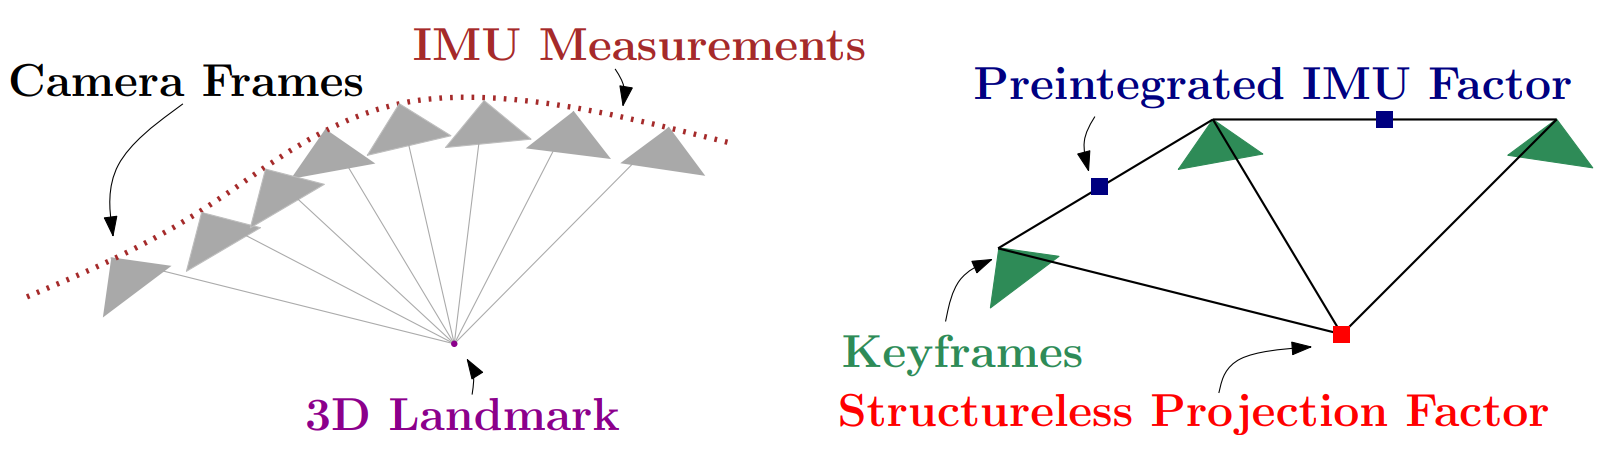
\includegraphics[width=\linewidth]{3-SLAM/3-related-work/figures/imuPreintegration.png}
    \caption{Illustration of on-manifold IMU pre-integration within a sensor-fusion odometry pipeline. Left: raw camera frames and high-frequency inertial measurements arriving asynchronously between keyframes. Right: the equivalent factor graph, in which the batch of intermediate IMU readings between two keyframes is compressed into a single pre-integrated IMU factor, while a structureless vision factor jointly constrains keyframes sharing observations of the same landmark \protect\cite{forsterOnManifoldPreintegrationRealTime2017}.}
    \label{fig:imuPreintegration}
\end{figure}

The result of this evolution is LIO-SAM \cite{shanLIOSAMTightlycoupledLidar2020}, which established the feature-based factor graph benchmark for global consistency, as shown in \cref{fig:liosamArchitecture}. LIO-SAM builds a factor graph incorporating LiDAR odometry, IMU pre-integration, and explicit loop closure factors. To manage computational complexity, it employs a ``sliding window'' local map for scan-to-map matching. Despite its accuracy and robustness compared with its predecessors, its reliance on LOAM-style feature extraction and a standard KD-tree for neighbour searching limits its performance in geometrically degenerate environments.

\begin{figure}[htbp]
    \centering
    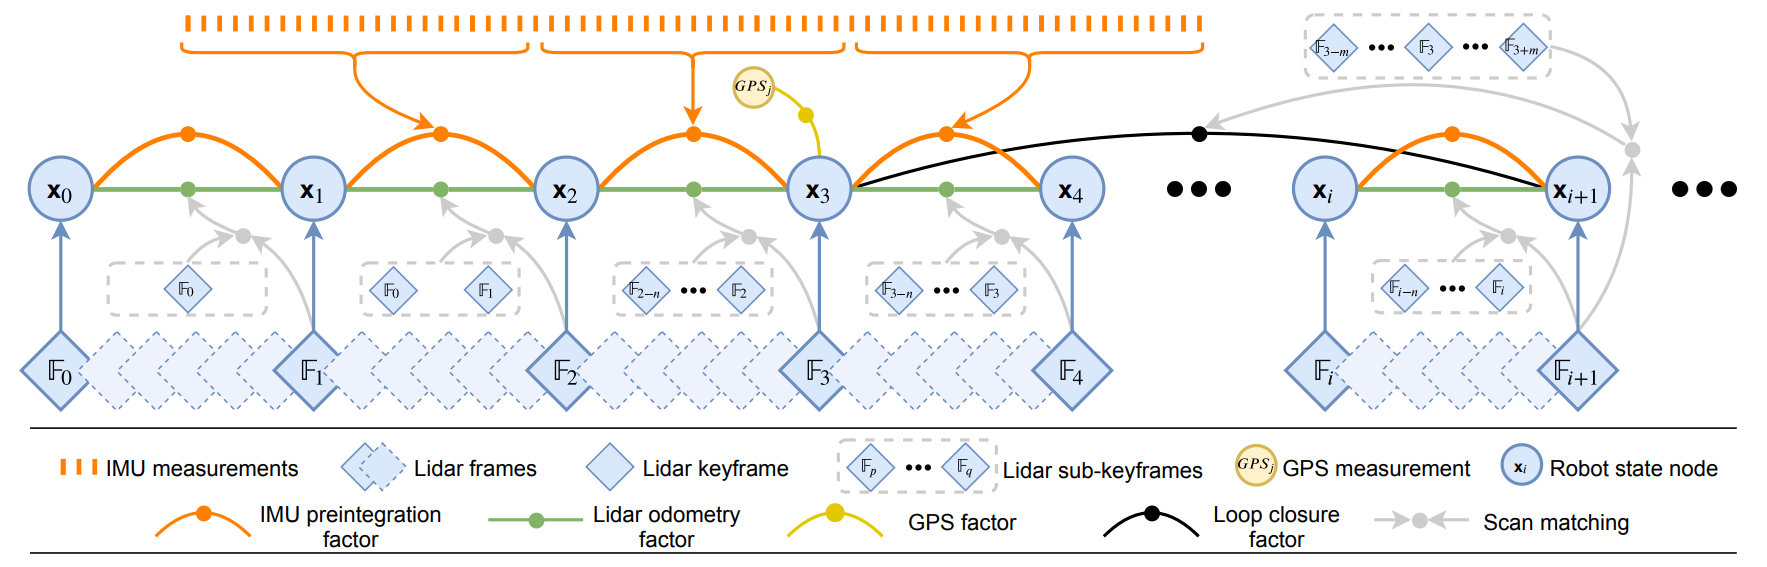
\includegraphics[width=0.85\linewidth]{3-SLAM/3-related-work/figures/LIO_SAM_Archictecture.png}
    \caption{Architecture of the LIO-SAM tightly-coupled LiDAR-inertial odometry framework. Inputs from a 3D LiDAR, an IMU, and an optional GPS receiver are fused within a factor graph composed of four distinct constraint types: IMU pre-integration factors linking consecutive keyframes, LiDAR odometry factors derived from scan-to-local-map registration, GPS absolute-position factors, and loop closure factors that suppress long-term drift \protect\cite{shanLIOSAMTightlycoupledLidar2020}.}
    \label{fig:liosamArchitecture}
\end{figure}

At the time of writing, the state of the art is defined by two architectural tracks: those prioritising extreme computational efficiency via filtering, and those prioritising global consistency and robustness via dense graph optimisation.

\paragraph{Filter-Based Direct Odometry}
Algorithms in the embedded track are designed to minimise CPU usage, making them suitable for low-power ARM processors on platforms like small drones. These systems rely on the Error-State Kalman Filter (ESKF) and are primarily odometry engines that estimate state and covariance, but are susceptible to drift over time as past states are marginalised.

FAST-LIO2 \cite{xuFASTLIO2FastDirect2022} is a widely adopted benchmark for computational efficiency, eschewing feature extraction in favour of registering raw points directly. Its two principal innovations are the Incremental KD-Tree (iKD-Tree), which supports dynamic map updates with amortised $O(\log N)$ complexity, and a Kalman Gain Inversion that reduces the filter update cost from the measurement dimension to the 18-dimensional state vector, enabling kHz-rate processing on modest hardware. Point-LIO \cite{hePointLIORobustHighBandwidth2023} extends this design by updating the EKF state for every individual point as it arrives from the sensor, yielding a processing bandwidth bounded only by the sensor's sampling rate. This point-wise update strategy enables tracking under aggressive motion where conventional scan-accumulation methods fail due to intra-frame distortion. Super-LIO \cite{wangSuperLIORobustEfficient2025} represents the most recent advance in this track, targeting the map data structure rather than the estimator itself. It introduces the \textbf{OctVox} representation — a hybrid combining a spatial hash map with internal octrees — to enforce strict point density constraints, and pairs this with a Heuristic-Guided $k$-Nearest Neighbour (HKNN) search that further reduces per-scan processing time. Reported benchmarks indicate lower CPU utilisation than FAST-LIO2, suggesting OctVox-based representations may define the next generation of resource-constrained LIO.

\paragraph{Graph-Based Global Consistency}
Systems in this track prioritise long-term mapping quality and robustness by leveraging high-performance hardware, particularly embedded GPUs.

GLIM (Global LiDAR Inertial Mapping) \cite{koideGLIM3DRangeInertial2024} represents a distinct departure from CPU-centric design, instead leveraging GPU parallelism to achieve dense, globally consistent mapping, as shown in \cref{fig:glimFramework}. Scan matching in GLIM is implemented via GPU-accelerated Voxelised Generalised Iterative Closest Point (VGICP) factors, which allow the system to incorporate nearly all points per frame and thereby retain geometric constraints that feature-based methods routinely discard. A further key contribution is the Submap Endpoint Mechanism, in which IMU pre-integration factors are inserted as stiff constraints on unobservable degrees of freedom within each submap. This structural guarantee preserves registration quality even when the LiDAR geometry is degenerate — for example in featureless tunnels or elevator shafts. For back-end estimation, GLIM employs a fixed-lag smoother that continuously optimises a bounded window of recent poses, combining the accuracy benefits of iterative re-linearisation with bounded memory consumption, in contrast to full-history SLAM approaches.

\begin{figure}
    \centering
    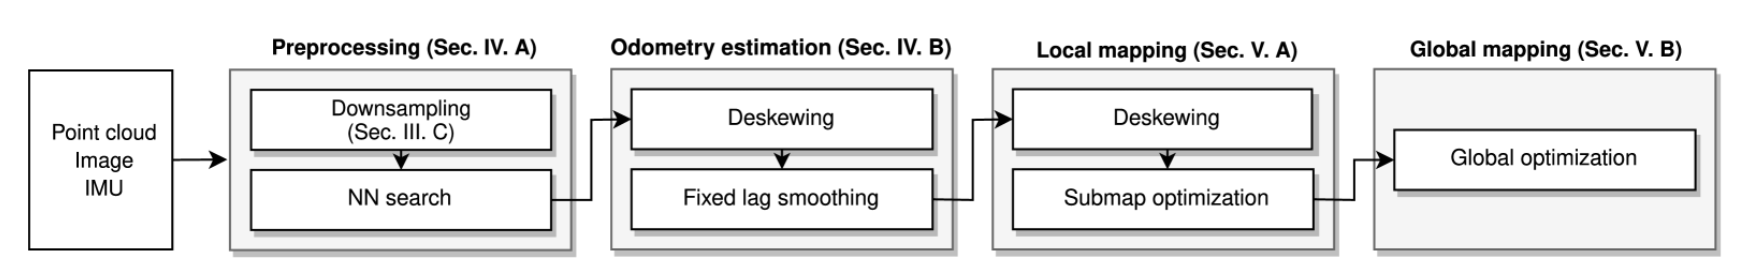
\includegraphics[width=0.9\linewidth]{3-SLAM/3-related-work/figures/glimFramework.png}
    \caption{Overview of the GLIM framework, comprising a preprocessing module and three tightly coupled range-IMU estimation modules. The odometry estimation module deskews point clouds and estimates sensor motion via fixed-lag smoothing; the local mapping module concatenates frames into submaps; and the global mapping module optimises submap poses for long-term global consistency. Each module runs in a dedicated thread \protect\cite{koideGLIM3DRangeInertial2024}.}
    \label{fig:glimFramework}
\end{figure}

This trade-off between computational efficiency and global consistency is summarised in the comparison table below. The most significant recent innovations have occurred in the map data structure domain (iKD-Tree, OctVox) for the filter-based track, and in hardware-software co-design (GLIM's GPU acceleration) for the graph-based track.

\begin{table}[htbp]
\centering
\caption{Comparative Analysis of State-of-the-Art LIO Systems}
\label{tab:comparison}
\small 
\renewcommand{\arraystretch}{1.3} 
\begin{tabular}{@{} l l l c l l @{}}
\toprule
\textbf{Algorithm} & \textbf{Backend} & \textbf{Map Structure} & \begin{tabular}[c]{@{}c@{}}\textbf{Loop}\\\textbf{Closure}\end{tabular} & \begin{tabular}[c]{@{}l@{}}\textbf{Robustness}\\\textbf{(Degeneracy)}\end{tabular} & \begin{tabular}[c]{@{}l@{}}\textbf{Efficiency}\\\textbf{(CPU)}\end{tabular} \\
\midrule
LIO-SAM    & Factor Graph   & Static KD-Tree & Yes & Moderate       & Low             \\
FAST-LIO2  & Iterated ESKF  & iKD-Tree       & No  & High (Direct)  & High            \\
Point-LIO  & Iterated ESKF  & iKD-Tree       & No  & Very High      & Moderate        \\
DLIO       & Geometric Obs. & KD-Tree/iVox   & No  & High           & High            \\
GLIM       & Factor Graph   & GPU Voxelmap   & Yes & \textbf{Extreme} & Low (GPU)       \\
Super-LIO  & Iterated ESKF  & \textbf{OctVox} & No  & High           & \textbf{Very High} \\
\bottomrule
\end{tabular}
\end{table}

Super-LIO is effective for projects constrained to low-power CPUs that can tolerate bounded drift, while GLIM excels at high-fidelity mapping applications where long-term global consistency and robustness to severe degeneracy are paramount, provided a GPU accelerator is available.

\subsection{SLAM Hyperparameter Optimisation}
\label{subsec:slam-hyperparameter}
As hyperparameter optimisation constitutes a primary contribution of this work (see \cref{sec:slam-intro}), this subsection surveys the relevant literature in greater depth than the architecture review above.
The optimisation of SLAM systems has evolved from manual tuning into rigorous hyperparameter optimisation (HPO) and statistical space exploration. In challenging real-world deployments such as agricultural settings, stability, robustness and generalisation become critical design objectives \cite{khanReviewSLAMTechniques2025}. Many modern SLAM systems utilise a complex set of interdependent parameters across the full pipeline, from feature extraction to back-end optimisation. Even focused subsystems such as loop-closure detection can depend strongly on multiple interacting parameters~\cite{hanMultiObjectiveOptimizationLoop2020}. The challenge of configuring a high-dimensional space, often referred to as the curse of dimensionality, poses a significant hurdle in tuning these SLAM systems. The first challenge is finding a subset of points from a high-dimensional search space that accurately represents the underlying performance landscape. 

\paragraph{Search Space Sampling}
One such method for sampling high-dimensional search spaces is Latin Hypercube Sampling (LHS). LHS, as formally introduced by Michael McKay in 1979, was used as a variance reduction technique to address the inefficiencies of Monte Carlo simulation (MCS) in high-dimensional domains \cite{chrismanLatinHypercubeSampling2014}. In MCS, sample points are generated independently, which often leads to ``clusters'' and ``voids'' in disparate regions, which can neglect critical narrow regions of optimal performance \cite{deutschLatinHypercubeSampling2012}. LHS addresses this by enforcing a stratification of the marginal distributions of each input variable.

LHS divides the range of each of the $d$ variables into $n$ equiprobable intervals. In a standard uniform distribution of $[0, 1]$, these strata are defined as $A_i = \left( \frac{i-1}{n}, \frac{i}{n} \right]$ for $i = 1, \dots, n$ \cite{chrismanLatinHypercubeSampling2014}. To generate a LHS sample, one value is drawn from each interval for each dimension. These values are then combined into vectors such that
each $n$ sample point is the only representative in each axis-aligned hyperplane. A visual comparison of MCS and LHS point distributions is shown in \cref{fig:samplingComparison}, and a comparison of LHS, MCS and Grid Search is detailed in \cref{tab:sampling_comparison}.

\begin{table}[h]
\centering
\small
\renewcommand{\arraystretch}{1.5}
\begin{tabularx}{\textwidth}{@{} >{\bfseries}l X X X @{}}
\toprule
Sampling Attribute & \textbf{Monte Carlo (MCS)} & \textbf{Grid Search} & \textbf{Latin Hypercube (LHS)} \\ 
\midrule
Variable Coverage & Random; susceptible to clustering & Uniform but sparse for high $d$ & Guaranteed univariate uniformity \cite{chrismanLatinHypercubeSampling2014} \\ 
\addlinespace
Sample Efficiency & Low; requires large $n$ for stability & Very low; $n^d$ scaling & High; independent of $d$ \cite{deutschLatinHypercubeSampling2012} \\ 
\addlinespace
Bias/Variance & Unbiased; high variance & Biased to grid points & Consistent; asymptotically unbiased \cite{packhamLatinHypercubeSampling2008} \\ 
\addlinespace
Search Structure & Unstructured & Rigidly structured & Near-random with low discrepancy \cite{chrismanLatinHypercubeSampling2014} \\ 
\bottomrule
\end{tabularx}
\caption{Comparison of Sampling Strategies}
\label{tab:sampling_comparison}
\end{table}

\begin{figure}[htbp]
    \centering
    \begin{subfigure}[b]{0.48\linewidth}
        \centering
        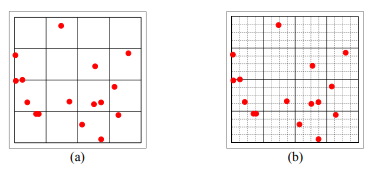
\includegraphics[width=\linewidth]{3-SLAM/3-related-work/figures/MC_dist.png}
        \caption{Monte Carlo sampling}
        \label{fig:mcDist}
    \end{subfigure}
    \hfill
    \begin{subfigure}[b]{0.48\linewidth}
        \centering
        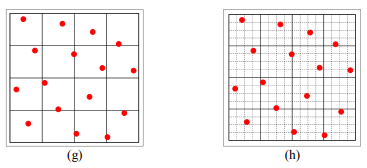
\includegraphics[width=\linewidth]{3-SLAM/3-related-work/figures/LHS_dist.png}
        \caption{Latin Hypercube sampling}
        \label{fig:lhsDist}
    \end{subfigure}
    \caption{Spatial distribution of 16 sample points drawn in a two-dimensional parameter space. In~\subref{fig:mcDist}, pure Monte Carlo sampling populates the space without structural constraint, producing irregular clusters and uncovered voids. In~\subref{fig:lhsDist}, the optimised Latin Hypercube Sampling stratification guarantee ensures that exactly one sample occupies each row and column of the partition grid, yielding substantially more uniform marginal coverage for the same number of evaluations \protect\cite{deutschLatinHypercubeSampling2012}.}
    \label{fig:samplingComparison}
\end{figure}

The advantage of LHS in SLAM parameterisation comes from its capacity to represent the parameter space with fewer samples than traditional methods. In a SLAM system with ten parameters, a grid search with only three levels per parameter would require $3^{10} = 59,049$ evaluations. Testing each sample on a real trajectory quickly becomes time prohibitive. LHS can explore the same search space with fewer points while maintaining that each parameter is tested at different levels \cite{deutschLatinHypercubeSampling2012}. Although uniformity is guaranteed across each axis, this does not guarantee that the interior of the hypercube is filled uniformly. As a result, researchers have developed Latin Hypercube Sampling with Multidimensional Uniformity (LHSMDU) to address the limitations of univariate stratification \cite{deutschLatinHypercubeSampling2012}. LHSMDU employs a sequential elimination process, where a large pool of MCS candidates are generated, and those that are too close in the multidimensional space are pruned \cite{deutschLatinHypercubeSampling2012}. This method maximises the minimum inter-point distance, maximising the spread of samples throughout the multi-dimensional space.

Often the SLAM parameters have physical or co-dependent constraints, such as turn radii or computational resource limits.
Standard LHS assumes independent variables, but extensions like Latin Hypercube Sampling with Dependence (LHSD) allow for the incorporation of copula-based dependence structures \cite{packhamLatinHypercubeSampling2008}. This method enforces constraints on the sampling strategy so that the search does not enter undefined/invalid regions of the search space. 

\paragraph{Robustness, Generalisation and Overfitting}
Finding a high-performance SLAM configuration for a single dataset is straightforward; the challenge is finding one that generalises across diverse environments. Single-dataset optimisation tends to overfit to the specific noise realisations and environmental characteristics of that sequence~\cite{koideAdaptiveHyperparameter2021}. A parameter set tuned for a feature-rich, static environment may adopt aggressive matching thresholds that cause tracking loss or false loop closures in open terrain with sparse landmarks. Environmental factors such as lighting variation, dynamic objects, geometric degeneracy, and platform speed each affect visual and LiDAR SLAM differently, making cross-environment robustness a fundamental constraint on the optimisation strategy. Bayesian optimisation approximates the objective with a probabilistic surrogate and selects evaluation points to maximise expected improvement, providing a sample-efficient, gradient-free framework for this cross-environment hyperparameter search~\cite{kandasamyTuningHyperparametersGrad}. This motivates the multi-dataset consensus framework developed in \cref{subsec:robust-slam-param}, which evaluates candidate configurations across multiple trajectories to penalise over-specialisation.

\clearpage

\section{Proposed Methods}
\label{sec:slam-methodology}

The following subsections describe the methods developed and integrated to achieve globally consistent, ENU-referenced localisation in vineyard environments. These contributions build on the GLIM framework surveyed in the preceding section and address the key challenges of reference frame alignment, GNSS outlier rejection, and parameter optimisation.

To begin this investigation, we implemented GLIM \cite{koideGLIM3DRangeInertial2024}. We chose GLIM as it had infrastructure in place to add extension modules to incorporate new sensors and capabilities. GLIM provides a global callback slot mechanism that allows access to the internal states of the mapping process and insertion of additional constraints into the factor graph. GLIM also eliminated sensor-specific processes, meaning it can be applied to a wide variety of range sensors such as spinning-type LiDAR, non-repetitive scan LiDAR, solid-state LiDAR and even RGB-D cameras.

GLIM state estimation is created in the local odometry frame. For our use in the wider research project, we required state estimation in the local ENU reference frame, which is a surveyed-in point at each of our farms. Thus, we needed a procedure to align the GLIM reference frame with the existing local ENU reference frame.

Firstly, we time synchronise the on-board GPS unit with the LiDAR and with the system clock. This allows us to associate corresponding GNSS points with the submaps or keyframes of LiDAR frames that GLIM registers, as illustrated in \cref{fig:time-matching}. We aggregate a set of corresponding GNSS coordinates with keyframe coordinates, and then implement the Kabsch algorithm \cite{kabschSolutionBestRotation1976} to find the relative transform between the two point sets by minimising the root-mean-square deviation between the two point sets.

\begin{figure}[htbp]
    \centering
    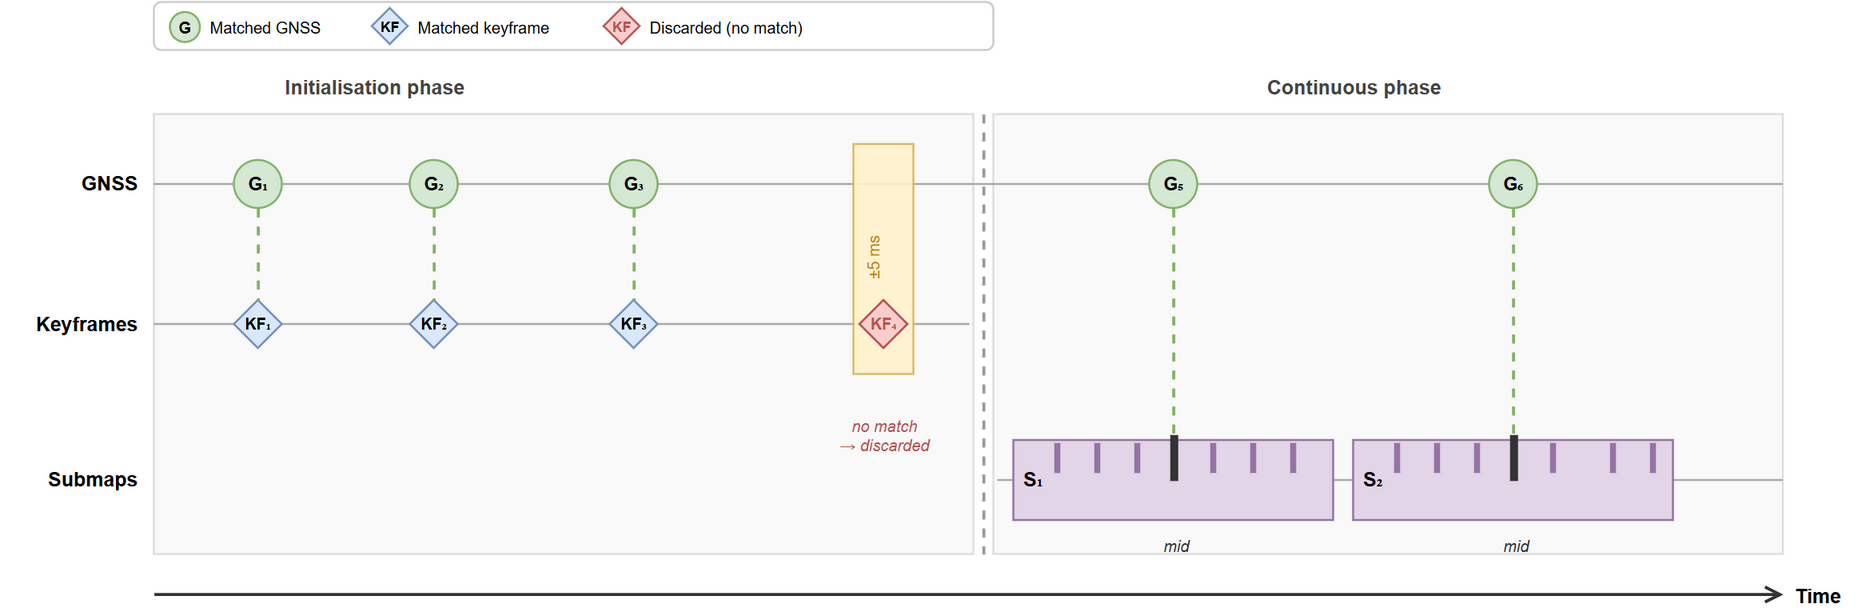
\includegraphics[width=\linewidth]{3-SLAM/3-methodology/figures/time-matching}
    \caption{GNSS-to-frame time matching across both operating phases. During the initialisation phase, each keyframe (KF) is matched to a GNSS measurement within a $\pm5$\,ms window enforced by PTP/Chrony clock synchronisation. A keyframe with no GNSS measurement in its window is discarded. During the continuous phase, submaps are matched using the timestamp of their middle keyframe (\textit{mid}), which approximates the temporal centroid of the submap.}
    \label{fig:time-matching}
\end{figure}

The Kabsch algorithm relies on the least-squares method to minimise the root-mean-square deviation (RMSD) between two point sets. Since the objective function squares the distances between paired points, outliers produce disproportionately large influences on the final transformation matrix. Thus, for global alignment, it is important that outliers are filtered out before executing the Kabsch algorithm. \cref{fig:system-pipeline} illustrates the complete proposed pipeline from sensor input to globally consistent ENU trajectory output.

\begin{figure}[htbp]
    \centering
    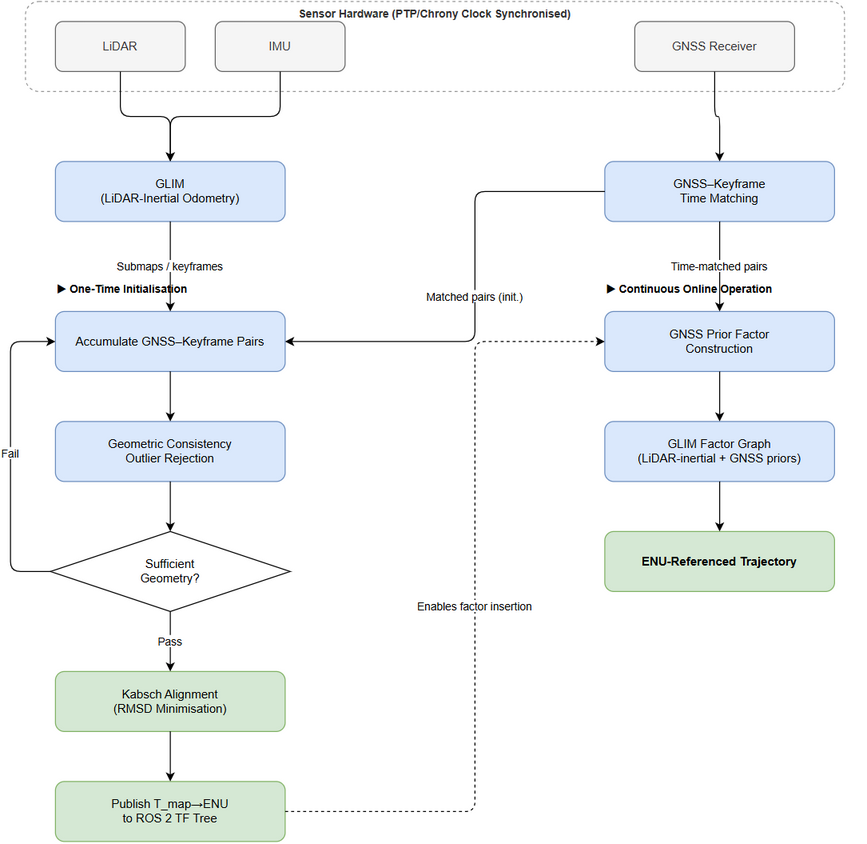
\includegraphics[width=\linewidth]{3-SLAM/3-methodology/figures/system-pipeline}
    \caption{Overview of the proposed GNSS-augmented SLAM pipeline. The initialisation track (left) performs time synchronisation, outlier rejection, planar geometry quality assessment, and Kabsch alignment to publish the map-to-ENU transform. The continuous track (right) constructs GNSS prior factors and inserts them into the GLIM factor graph for ongoing drift correction. On geometry check failure, initialisation waits and accumulates further GNSS--pose correspondences before retrying.}
    \label{fig:system-pipeline}
\end{figure}

\subsection{Geometric Consistency-Based Outlier Rejection}

To remove spurious GNSS measurements prior to initialisation, we apply a geometric consistency check that exploits the rigidity of the GNSS--IMU transformation. The method assumes that, for inlier measurements, pairwise distances between GNSS observations should be preserved when mapped into the local map frame via the estimated poses.

Let $\{\mathbf{g}_i\}_{i=1}^{N}$ denote GNSS positions expressed in the ENU frame, and $\{\hat{\mathbf{g}}_i\}_{i=1}^{N}$ denote the corresponding GNSS positions expressed in the map frame, obtained by transforming IMU poses with a fixed extrinsic calibration. For each point $i$, we evaluate its consistency with all other points $j \neq i$ by comparing pairwise Euclidean distances in both frames as shown in Equation \eqref{eq:consistency_check}:
\begin{equation}
\label{eq:consistency_check}
\left| \lVert \mathbf{g}_i - \mathbf{g}_j \rVert - \lVert \hat{\mathbf{g}}_i - \hat{\mathbf{g}}_j \rVert \right| < \tau,
\end{equation}
where $\tau$ is a distance consistency threshold reflecting accepted SLAM error and GNSS noise.

This approach was chosen over stochastic methods like RANSAC \cite{fischlerRandomSampleConsensus1981} or iterative M-estimators because it takes advantage of the invariance of pairwise Euclidean distances under rigid body transformations, which means that the method remains entirely deterministic and independent of any initial pose estimate or probabilistic modelling.

To formalise the inlier classification, we define a pairwise consistency indicator $c_{ij}$ in Equation \eqref{eq:indicator}:
\begin{equation}
\label{eq:indicator}
c_{ij} = 
\begin{cases} 
1 & \text{if } \left| \lVert \mathbf{g}_i - \mathbf{g}_j \rVert - \lVert \hat{\mathbf{g}}_i - \hat{\mathbf{g}}_j \rVert \right| < \tau \\
0 & \text{otherwise}
\end{cases}
\end{equation}
A measurement is classified as an inlier if the fraction of other points with which it satisfies the above constraint exceeds a minimum inlier ratio $\rho$, satisfying the condition:
\begin{equation}
\label{eq:majority_criterion}
\frac{1}{N-1} \sum_{j \neq i}^{N} c_{ij} > \rho.
\end{equation}

GNSS multipath errors \cite{wenExclusionGNSSNLOS2018} can often create erroneous clusters of points that are mutually consistent, and therefore are not filtered out by conventional statistical outlier methods. However, the majority-based criterion in Equation \eqref{eq:majority_criterion} ensures that points are only kept if they belong to the global rigid consensus, effectively filtering out clusters of mutually consistent but globally erroneous points. After classification, only inlier GNSS measurements and their corresponding map-frame estimates are preserved for subsequent processing. \cref{fig:outlier-rejection} illustrates a representative scenario in which inlier measurements lie along the physical trajectory while a multipath cluster is correctly rejected.

\begin{figure}[htbp]
    \centering
    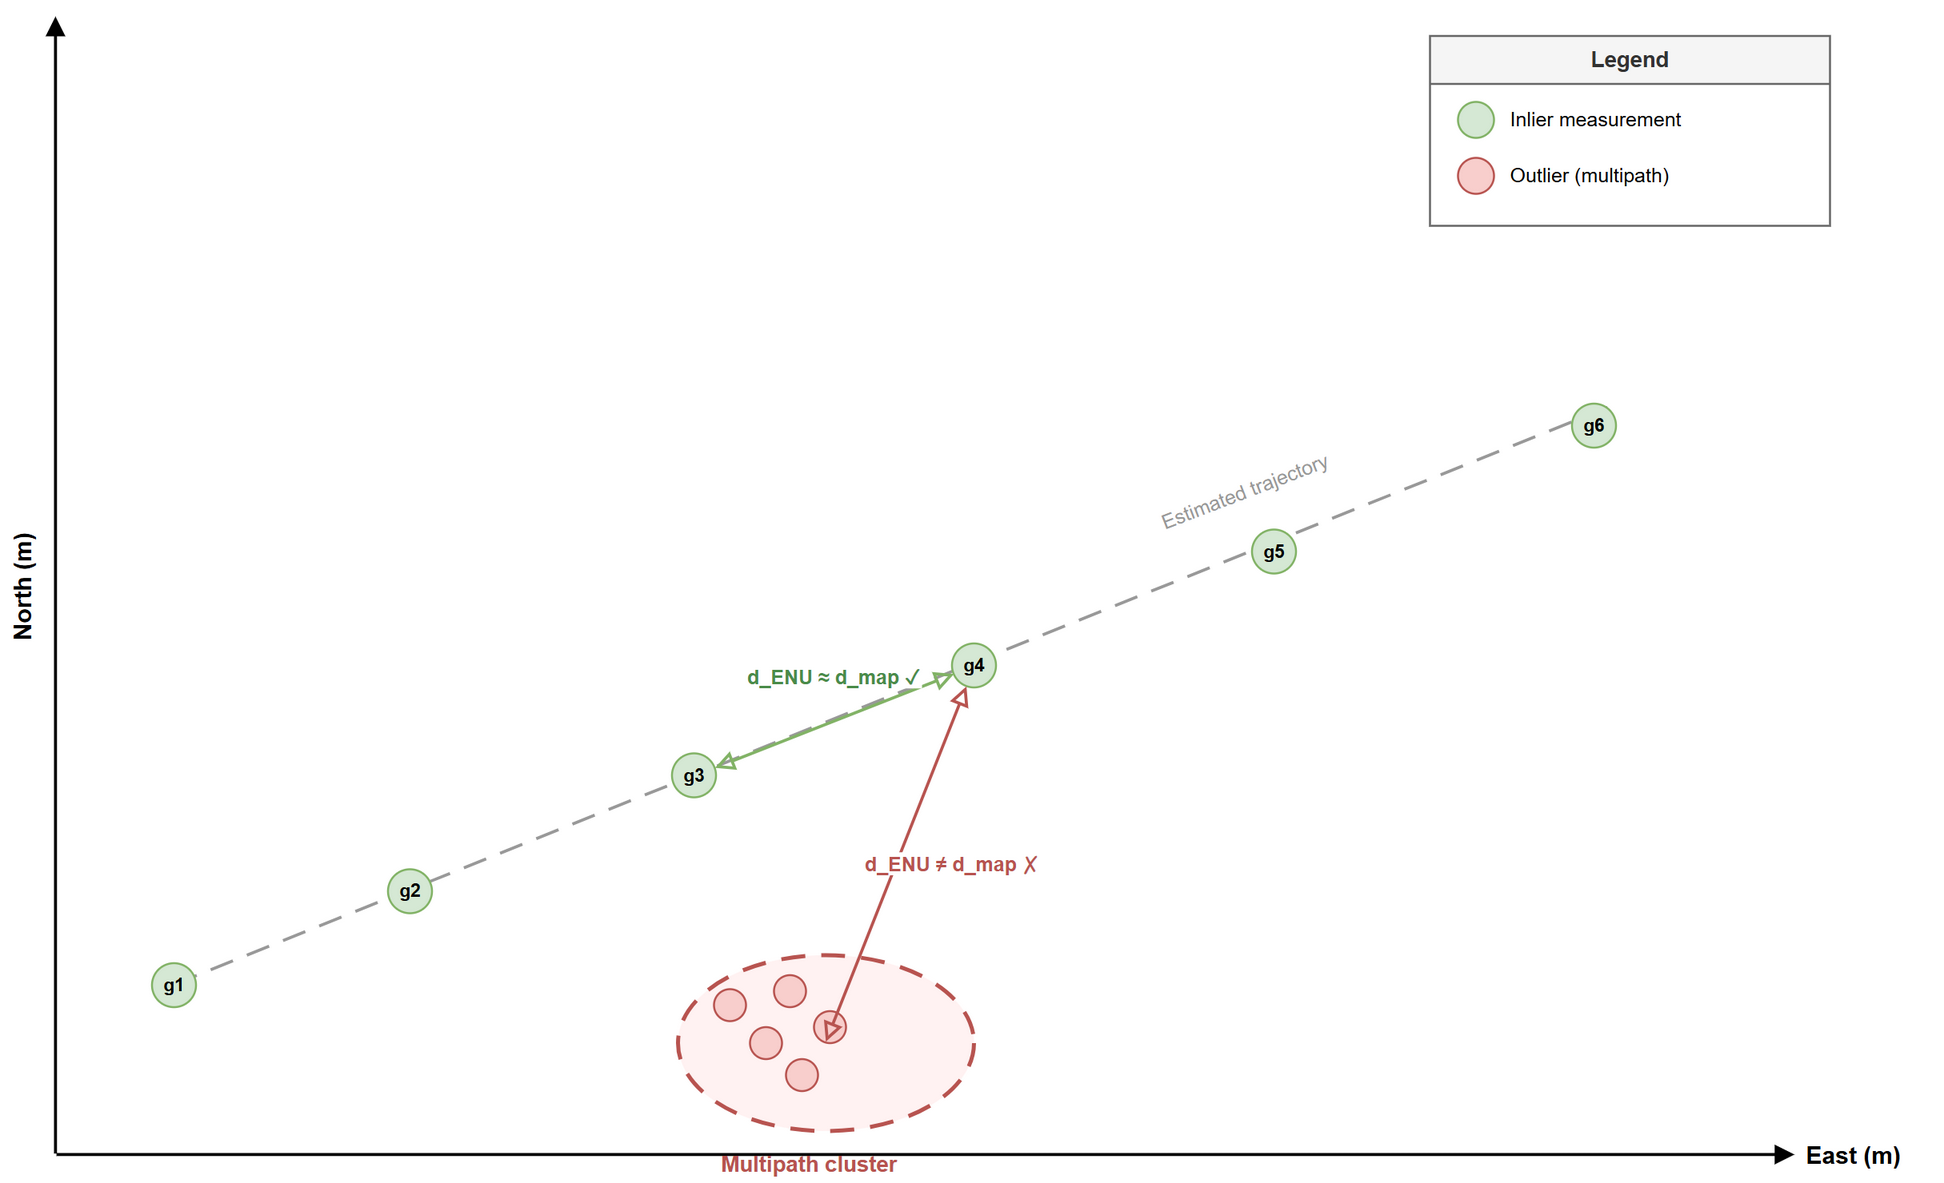
\includegraphics[width=0.75\linewidth]{3-SLAM/3-methodology/figures/outlier-rejection}
    \caption{Geometric consistency-based outlier rejection applied to GNSS measurements. Inlier points (green) are distributed along the estimated trajectory and satisfy pairwise distance consistency with map-frame estimates. Multipath-corrupted points (red) form a spatially compact cluster that is globally inconsistent with the rigid consensus and are therefore rejected, even though they are mutually self-consistent.}
    \label{fig:outlier-rejection}
\end{figure}

\subsection{Planar Geometry Quality Assessment in 2D}

Subsequently to outlier rejection, we assess the geometric quality of the remaining point set under the assumption of planar motion by analysing its distribution in the horizontal plane. This analysis is motivated by the sensitivity of the Kabsch algorithm to degenerate point configurations: near-collinear or poorly distributed trajectories produce ill-conditioned cross-covariance matrices, leading to unstable or biased transformations. By detecting such configurations before alignment, we ensure the SVD is well-conditioned and that the estimated transformation is numerically reliable. In particular, we enforce minimum requirements on translational baseline ($\geq 5.0\,\mathrm{m}$), planar spread, rotational excitation, and numerical conditioning.

Given a set of 3D points $\{\mathbf{p}_i\}_{i=1}^{N}$, only the horizontal components are considered by projecting each point onto the $xy$-plane, yielding $\mathbf{q}_i = [x_i, y_i]^\top$. If fewer than three points are available, the geometry is deemed insufficient and the assessment terminates early.

The projected points are assembled into a data matrix $\mathbf{M}$ as defined in Equation \eqref{eq:data_matrix}:
\begin{equation}
\label{eq:data_matrix}
\mathbf{M} = \begin{bmatrix}
\mathbf{q}_1 & \mathbf{q}_2 & \cdots & \mathbf{q}_N
\end{bmatrix} \in \mathbb{R}^{2 \times N},
\end{equation}
which is centred by subtracting the mean $\bar{\mathbf{q}}$ from each column. Singular value decomposition is then applied to the centred matrix as shown in Equation \eqref{eq:svd}:
\begin{equation}
\label{eq:svd}
\mathbf{M} = \mathbf{U} \boldsymbol{\Sigma} \mathbf{V}^\top,
\end{equation}
yielding two singular values $\sigma_1 \geq \sigma_2$ that characterise the principal spatial extents of the trajectory in the plane.

The condition number $\kappa$ is defined in Equation \eqref{eq:condition_number}:
\begin{equation}
\label{eq:condition_number}
\kappa = \frac{\sigma_1}{\sigma_2},
\end{equation}
and is used as a degeneracy metric, with large values indicating near-collinear motion. The geometry is considered non-degenerate if $\kappa < 20.0$.

To evaluate spatial coverage, a 2D spread ratio $r$ is computed according to Equation \eqref{eq:spread_ratio}:
\begin{equation}
\label{eq:spread_ratio}
r = \frac{\sigma_2}{\sigma_1},
\end{equation}
which measures how well the trajectory excites both planar directions. A minimum spread ratio of $r \geq 0.15$ is required. Additionally, a minimum displacement constraint is enforced by requiring both singular values to exceed a baseline threshold of $5.0\,\mathrm{m}$. The spatial distribution is considered sufficient only if both the spread ratio and displacement conditions are satisfied.

Rotational excitation is evaluated independently by computing the angular span of the point set in the horizontal plane. The geometry is considered to provide sufficient rotational constraint if the angular span exceeds $45.0^\circ$.

The final geometry quality assessment combines these criteria, reporting whether the point set exhibits sufficient planar spread, adequate rotational excitation, and non-degenerate conditioning. This 2D-based evaluation provides a robust and numerically stable measure of geometric suitability for planar motion scenarios. \cref{fig:geometry-quality} contrasts a degenerate near-collinear configuration against a well-conditioned L-shaped trajectory to illustrate the effect of point distribution on singular value spread.

\begin{figure}[htbp]
    \centering
    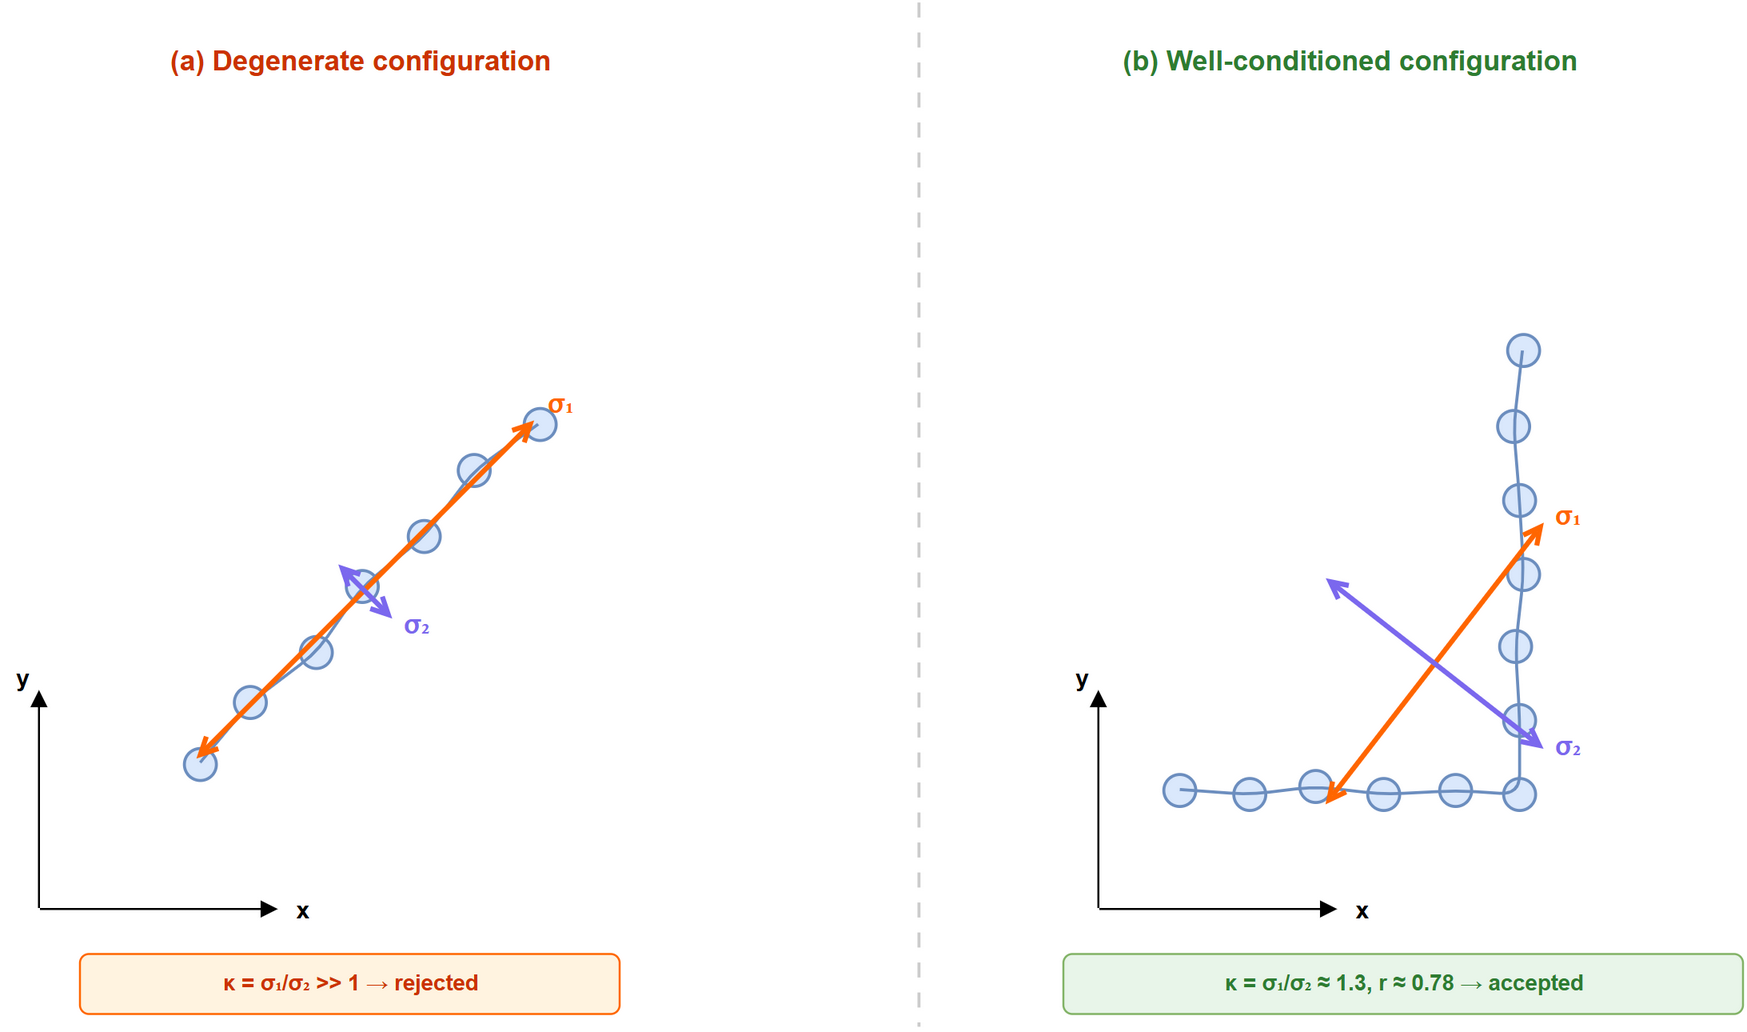
\includegraphics[width=0.85\linewidth]{3-SLAM/3-methodology/figures/geometry-quality}
    \caption{Planar geometry quality assessment for two trajectory configurations.
    \textbf{(a)}~Near-collinear configuration: points lie along a single direction,
    yielding a large condition number $\kappa \gg 1$, indicating insufficient geometric
    spread for reliable plane estimation.
    \textbf{(b)}~Well-conditioned configuration: an L-shaped trajectory distributes
    points across two directions, yielding $\kappa \approx 1.3$ and $r \approx 0.78$.
    Orange and purple arrows denote the first and second principal variance directions
    ($\sigma_1$, $\sigma_2$) obtained from SVD of the centred point set; their
    orientations reflect directions of maximum and minimum variance across all points
    and are not constrained to align with individual path segments.}
    \label{fig:geometry-quality}
\end{figure}

\subsection{GLIM Reference Frame Alignment with Local ENU}

Given two corresponding point sets $\{\mathbf{a}_i\}_{i=1}^N, \{\mathbf{b}_i\}_{i=1}^N \subset \mathbb{R}^3$, the goal is to estimate a rigid-body transformation $(\mathbf{R}, \mathbf{t}) \in \mathrm{SO}(3) \times \mathbb{R}^3$ that minimises the sum of squared alignment errors as defined in the following objective function:
\begin{equation}
\label{eq:kabsch_objective}
\min_{\mathbf{R}, \mathbf{t}} \sum_{i=1}^{N} \left\| \mathbf{b}_i - (\mathbf{R}\mathbf{a}_i + \mathbf{t}) \right\|^2, \quad \text{s.t. } \det(\mathbf{R}) = 1.
\end{equation}

First, the centroids of both point sets are computed as:
\begin{equation}
\label{eq:centroids}
\boldsymbol{\mu}_A = \frac{1}{N} \sum_{i=1}^N \mathbf{a}_i, \qquad \boldsymbol{\mu}_B = \frac{1}{N} \sum_{i=1}^N \mathbf{b}_i.
\end{equation}

The point sets are then centred by subtracting their respective centroids:
\begin{equation}
\label{eq:centering}
\tilde{\mathbf{a}}_i = \mathbf{a}_i - \boldsymbol{\mu}_A, \qquad \tilde{\mathbf{b}}_i = \mathbf{b}_i - \boldsymbol{\mu}_B.
\end{equation}

A $3 \times 3$ cross-covariance matrix $\mathbf{H}$ is formed as:
\begin{equation}
\label{eq:cross_covariance}
\mathbf{H} = \sum_{i=1}^N \tilde{\mathbf{b}}_i \tilde{\mathbf{a}}_i^{\top}.
\end{equation}

The singular value decomposition (SVD) of $\mathbf{H}$ is computed in Equation \eqref{eq:kabsch_svd}:
\begin{equation}
\label{eq:kabsch_svd}
\mathbf{H} = \mathbf{U} \boldsymbol{\Sigma} \mathbf{V}^{\top}.
\end{equation}

To ensure a proper rotation and avoid reflections, a diagonal correction matrix $\mathbf{D}$ is introduced:
\begin{equation}
\label{eq:reflection_correction}
\mathbf{D} = \mathrm{diag}(1,\,1,\,\mathrm{sign}(\det(\mathbf{U}\mathbf{V}^{\top}))).
\end{equation}

The optimal rotation $\mathbf{R}$ is then given by:
\begin{equation}
\label{eq:optimal_rotation}
\mathbf{R} = \mathbf{U}\mathbf{D}\mathbf{V}^{\top}.
\end{equation}

Finally, the translation $\mathbf{t}$ is recovered according to Equation \eqref{eq:recovered_translation}:
\begin{equation}
\label{eq:recovered_translation}
\mathbf{t} = \boldsymbol{\mu}_B - \mathbf{R}\boldsymbol{\mu}_A.
\end{equation}

The resulting rigid transformation $(\mathbf{R}, \mathbf{t})$ aligns the source point set to the target point set in a least-squares sense, as illustrated in \cref{fig:kabsch-alignment}. This static transformation is published to the ROS2 transform tree \cite{macenskiRobotOperatingSystem2022} to link the local ENU frame to the GLIM mapping frame.

\begin{figure}[htbp]
    \centering
    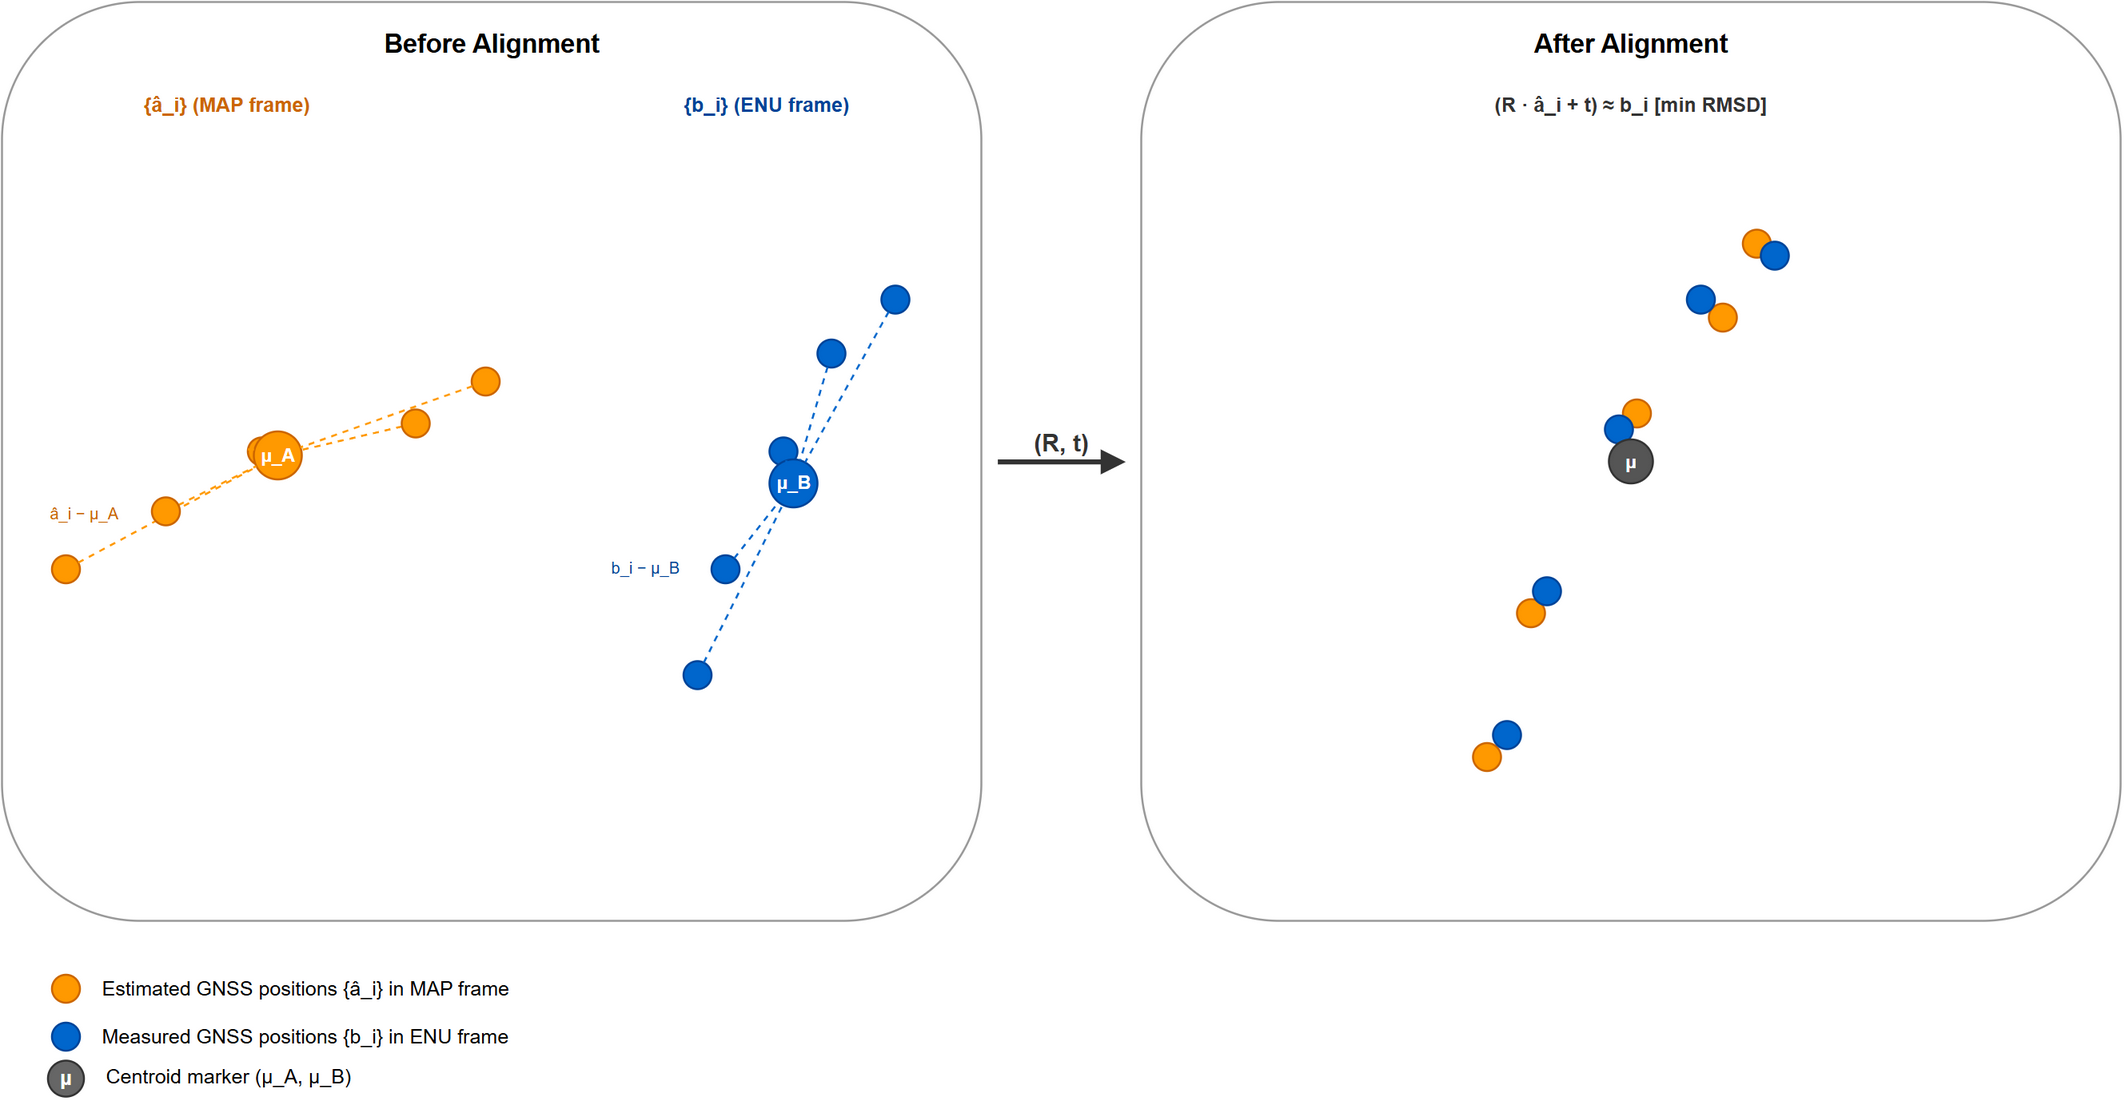
\includegraphics[width=\linewidth]{3-SLAM/3-methodology/figures/kabsch-alignment}
    \caption{Kabsch point-set alignment between estimated GNSS antenna positions $\{\hat{\mathbf{a}}_i\}$ in the MAP frame (orange) and measured GNSS positions $\{\mathbf{b}_i\}$ in the ENU frame (blue). \textit{Left}: before alignment, dashed lines show the centred vectors $\hat{\mathbf{a}}_i - \boldsymbol{\mu}_A$ and $\mathbf{b}_i - \boldsymbol{\mu}_B$ relative to their respective centroids. The clearly different orientations of the two point sets illustrate that the estimated transformation $(\mathbf{R}, \mathbf{t})$ must account for both a rotation and a translation (Equations~\eqref{eq:kabsch_objective}--\eqref{eq:recovered_translation}). \textit{Right}: after alignment, the transformed MAP-frame positions $\mathbf{R}\hat{\mathbf{a}}_i + \mathbf{t}$ coincide with the ENU measurements up to a small residual.}
    \label{fig:kabsch-alignment}
\end{figure}

\subsection{GNSS Prior Factor Construction}

This procedure augments an existing SLAM factor graph \cite{grisettiTutorialGraphBasedSLAM2010a} with GNSS-based prior constraints that relate submap poses to global position measurements. Each GNSS measurement is incorporated as a probabilistic constraint on the estimated submap pose through a known sensor extrinsic calibration.

Let $\mathbf{T}_{\text{map}}^{\text{enu}} \in SE(3)$ denote the rigid transformation from the local ENU frame to the GLIM map frame, and $\mathbf{p}_{\text{imu}}^{\text{gps}} \in \mathbb{R}^3$ the fixed translation from the IMU frame to the GNSS antenna frame. For each correspondence between a submap and a GNSS measurement, the following steps are performed.

First, the GNSS position $\mathbf{p}_{\text{enu}} \in \mathbb{R}^3$ is extracted in the ENU frame and transformed into the map frame as shown in Equation \eqref{eq:enu_to_map}:
\begin{equation}
\label{eq:enu_to_map}
\mathbf{p}_{\text{map}} = \mathbf{T}_{\text{map}}^{\text{enu}} \, \mathbf{p}_{\text{enu}}.
\end{equation}

Next, a diagonal Gaussian noise model is constructed from the reported GNSS covariance. Let $\boldsymbol{\sigma} \in \mathbb{R}^3$ denote the standard deviations obtained from the square root of the covariance diagonal. These values are scaled by a configurable factor $\alpha$ and converted to a covariance matrix in Equation \eqref{eq:gps_noise}:
\begin{equation}
\label{eq:gps_noise}
\boldsymbol{\Sigma}_{\text{gps}} = \mathrm{diag}\!\left((\alpha \boldsymbol{\sigma})^2\right).
\end{equation}

Given a submap pose $\mathbf{T}_{\text{map}}^{\text{sub}} \in SE(3)$, the predicted GNSS antenna position in the map frame is expressed in Equation \eqref{eq:predicted_gps}:
\begin{equation}
\label{eq:predicted_gps}
\hat{\mathbf{p}}_{\text{map}} = \mathbf{T}_{\text{map}}^{\text{sub}} \, \mathbf{p}_{\text{imu}}^{\text{gps}}.
\end{equation}
This formulation is valid as the GLIM submap origin is defined at the IMU center, such that the extrinsic offset $\mathbf{p}_{\text{imu}}^{\text{gps}}$ represents the antenna position relative to the submap origin. An expression-based factor is then constructed to minimize the residual between the predicted and measured positions under the noise model $\mathcal{N}(\mathbf{0}, \boldsymbol{\Sigma}_{\text{gps}})$:
\begin{equation}
\label{eq:gnss_factor}
\mathbf{r}(\mathbf{T}_{\text{map}}^{\text{sub}}) = \left\| \hat{\mathbf{p}}_{\text{map}} - \mathbf{p}_{\text{map}} \right\|^2_{\boldsymbol{\Sigma}_{\text{gps}}}.
\end{equation}

This factor directly constrains the corresponding submap pose variable in the factor graph, contributing to global consistency and LiDAR-inertial odometry drift correction. In effect, this factor constrains the GLIM-predicted position of the GPS antenna using the measured GNSS position at that time. \cref{fig:factor-graph} depicts the resulting factor graph structure, highlighting the asynchronous attachment of GNSS prior factors to submap pose nodes alongside the continuous LiDAR--IMU odometry chain.

\begin{figure}[htbp]
    \centering
    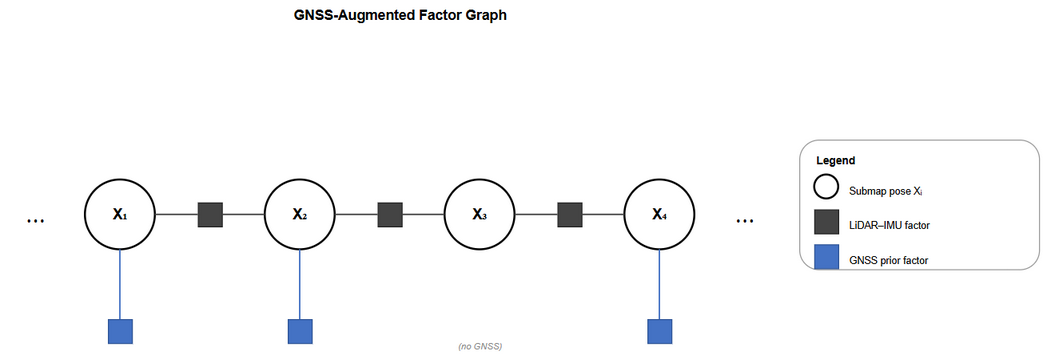
\includegraphics[width=0.85\linewidth]{3-SLAM/3-methodology/figures/factor-graph}
    \caption{GNSS-augmented factor graph structure. Circles denote submap pose variables $X_i$; dark squares represent LiDAR--IMU odometry factors between consecutive submaps; blue squares represent GNSS prior factors attached to corresponding submap poses. GNSS measurements arrive asynchronously and are therefore not associated with every submap (illustrated by the absent factor at $X_3$).}
    \label{fig:factor-graph}
\end{figure}

\subsection{Robust SLAM Parameterisation via Iterative Region Refinement}

The optimisation of Simultaneous Localisation and Mapping (SLAM) parameters is a high-dimensional, non-convex problem where the objective is to identify a parameter vector $\Theta$ that minimises localisation error across heterogeneous environments \cite{hanMultiObjectiveOptimizationLoop2020}. This subsection proposes a model-free, heuristic region-refinement algorithm that transitions from global stochastic exploration to localised deterministic refinement. The strategy assumes that optimal configurations cluster within specific sub-regions of the hyper-dimensional search space $\Omega$, which are iteratively identified and contracted using statistical distribution analysis.

\subsubsection{Problem Formulation}
We define the SLAM system as a complex function $f(X,\theta)$, where $X$ represents raw sensor data (e.g., LiDAR scans and inertial measurements) and $\Theta$ is the $d$-dimensional parameter vector. In a typical LiDAR-inertial setup, $\Theta$ includes parameters such as LiDAR resolution and registration strategy. The objective is to find $\Theta^*$ such that:
\begin{equation}
    \Theta^* = \arg\min_{\Theta \in \Omega} \mathcal{J}(\Theta)
\end{equation}
where $\mathcal{J}$ is a robust objective function representing the consensus performance across $K$ distinct motion profiles.

\subsubsection{Sampling via Latin Hypercube Strategy}
To explore the initial parameter manifold, we utilise Latin Hypercube Sampling (LHS) as an alternative to traditional grid search or independent Monte Carlo (MC) sampling \cite{deutschLatinHypercubeSampling2012}. LHS is technically categorised as a stratified sampling design \cite{chrismanLatinHypercubeSampling2014}. For a sample size $N$ in $d$ dimensions, the range of each parameter $\theta_j$ is partitioned into $N$ equiprobable intervals for $j=1, \dots, d$ \cite{chrismanLatinHypercubeSampling2014}. The mathematical constraint --- ensuring exactly one sample per row and column of the grid --- minimises the ``clustering'' phenomenon common in pure random sampling \cite{deutschLatinHypercubeSampling2012}. This stratification ensures that the marginal distribution of each parameter is sampled uniformly, achieving a lower variance than independent Monte Carlo sampling for the same sample size \cite{packhamLatinHypercubeSampling2008}.

\paragraph{Implementation and Normalisation}
Parameter vectors are first normalised to the unit hypercube $[0, 1]^d$ \cite{deutschLatinHypercubeSampling2012}. To ensure reproducibility, the pseudo-random permutations used to construct the hypercube are seeded deterministically. The samples are subsequently scaled to physical ranges using:
\begin{equation}
    \theta_{j,i} = \theta_{j, \min} + u_{j,i} (\theta_{j, \max} - \theta_{j, \min})
\end{equation}
where $\theta_{j, \min}$ and $\theta_{j, \max}$ represent the physical lower and upper bounds for parameter $j$.

\subsubsection{The Multi-Dataset Consensus Framework}
A primary challenge in SLAM optimisation is the risk of ``over-specialisation'', where parameters become overfitted to the unique noise characteristics of a single trajectory \cite{soaresVARSLAMVisualAdaptive2025}. We implement a Consensus Survival Framework to prioritise reliability across datasets.

In some situations, standard ``Mean-Performance Optimisation'' can hide brittle configurations that perform well on average but fail catastrophically on a single sequence \cite{kandasamyTuningHyperparametersGrad}. However, in this setting, catastrophic failure typically results in excessively high amplitude errors, which effectively inflate the mean normalised error. That being said, some particular parameter configurations can lead to excessive GPU draw, resulting in a runtime CUDA out-of-memory error. If the parameter set does not complete processing the trajectory on any dataset $k$, it is assigned an infinite cost and discarded from the survivor pool. This ensures the survival of only those configurations that meet the computational requirements of the system.

\paragraph{Formal Objective Function}
For the "surviving" configurations, the objective function $J(\theta)$ is defined as the mean normalized error across the valid sequences \eqref{eq:piecewise_success}:
\begin{equation}
\label{eq:piecewise_success}
J(\theta) = 
\begin{cases} 
\frac{1}{K} \sum_{k=1}^K E_k(\theta) & \text{if success} \in \{D_1, \dots, D_K\} \\ 
\infty & \text{otherwise} 
\end{cases}
\end{equation}

where $E_k(\theta)$ is the primary performance metric for dataset $k$.

\subsubsection{Iterative Region Refinement (IRR)}
The optimisation proceeds through an ``Iterative Contraction'' or ``Funnel'' strategy. This mirrors the reduction of a search radius in traditional Trust Region Methods \cite{nocedalTrustRegionMethods2006}, concentrating the sampling density into the most promising basins of attraction.

\paragraph{Statistical Search Space Contraction}
At the conclusion of each phase $i$, the top-performing configurations are used to calculate new search boundaries for phase $i+1$. We employ the 10th and 90th percentiles of the elite set as robust estimators for the update rule in Equation \eqref{eq:quantile_update}:
\begin{equation}
\label{eq:quantile_update}
\Omega_{j, i+1} = [P_{10}(\theta_{j, \text{top}}), P_{90}(\theta_{j, \text{top}})].
\end{equation}
This quantile-based reduction is superior to using absolute Min/Max values because it is resilient to ``lucky'' outliers --- configurations that may perform well due to noise interactions rather than parameter stability.

\paragraph{Refinement Phase Schedule}
The optimisation is structured into four phases, increasing the selection pressure (lower survival rate) as the search space contracts, as detailed in \cref{tab:phases}:

\begin{table}[h]
\centering
\caption{Evolutionary Phases of the Sampling Algorithm}
\label{tab:phases}
\begin{tabularx}{\textwidth}{@{} l l c c X @{}}
\toprule
\textbf{Phase} & \textbf{Objective} & \textbf{Iterations (N)} & \textbf{Survival Rate} & \textbf{Description} \\ \midrule
Phase 1 & Thinning & 100 & 30\% & Broad exploration identifying stable regions. \\
Phase 2 & Narrowing & 100 & 20\% & Convergence on local minima. \\
Phase 3 & Refinement & 100 & 10\% & High-density sampling within basins. \\
Phase 4 & Fine-tuning & 75 & 1.3\% & Final tuning to find top candidate. \\ \bottomrule
\end{tabularx}
\end{table}

This incremental strategy is distinct from Successive Halving (SHA) \cite{jamiesonNonstochasticBestArm2015}, as it preserves a continuous distribution of potential solutions rather than discarding them in discrete early-stopping steps, which is critical for SLAM where early performance does not always correlate with final drift. \cref{fig:irr-funnel} visualises the contracting search space across phases, showing how sample density converges toward the optimal configuration.

\begin{figure}[htbp]
    \centering
    \begin{subfigure}[t]{0.57\textwidth}
        \centering
        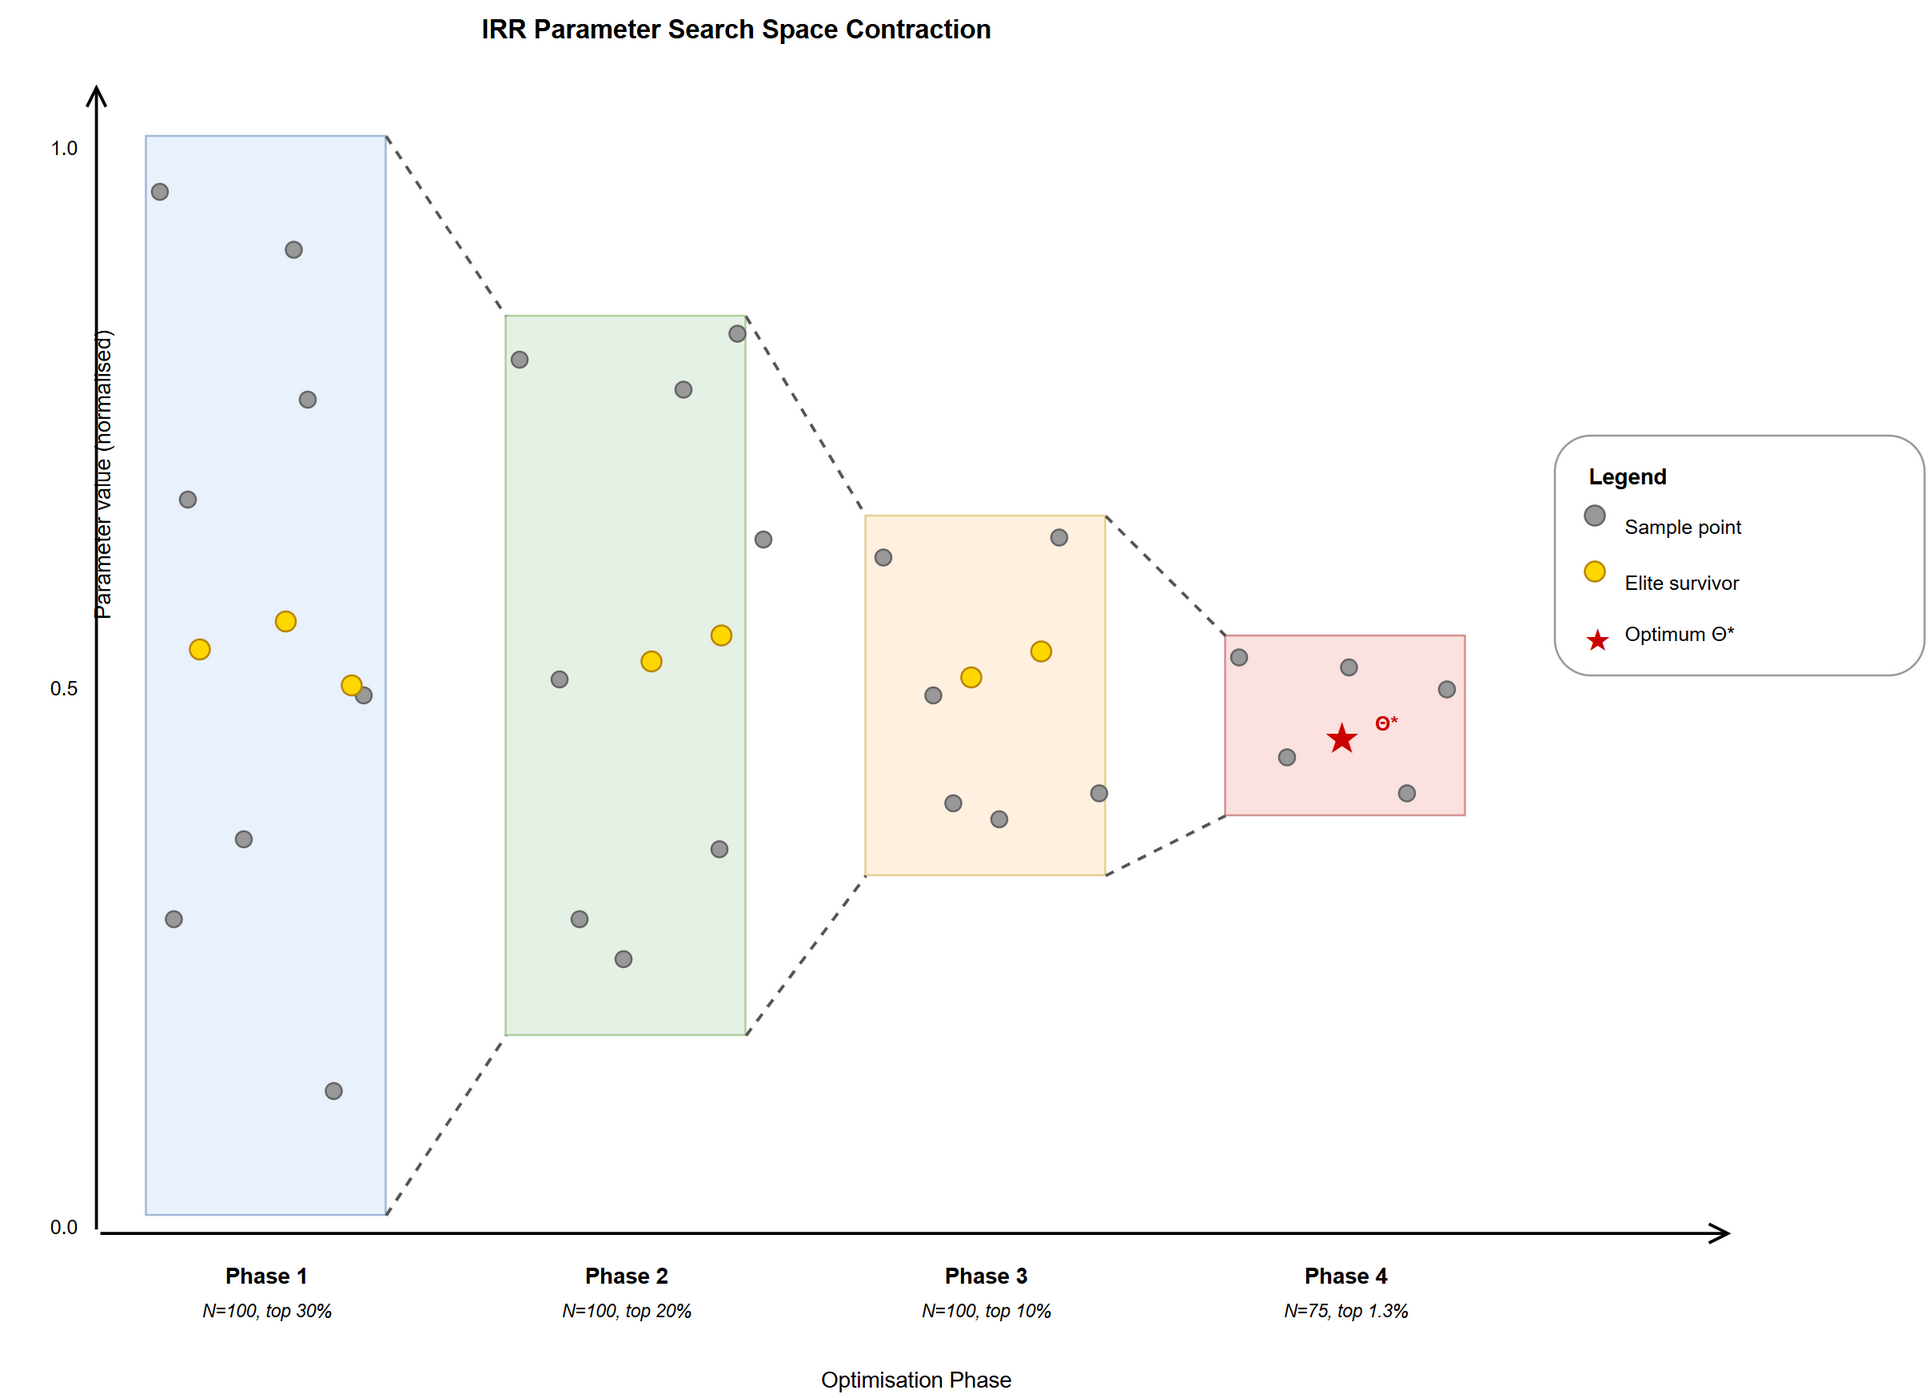
\includegraphics[width=\linewidth]{3-SLAM/3-methodology/figures/irr-funnel}
        \caption{Parameter search space contraction across four optimisation phases. Each coloured band represents the active search bounds for a single parameter dimension (normalised to $[0,1]$); bounds are updated between phases using the $P_{10}$--$P_{90}$ range of the elite survivor set (dashed diagonal lines). Grey dots are sampled configurations; gold dots are elite survivors; the red star marks the final optimum $\Theta^*$.}
        \label{fig:irr-funnel}
    \end{subfigure}
    \hfill
    \begin{subfigure}[t]{0.40\textwidth}
        \centering
        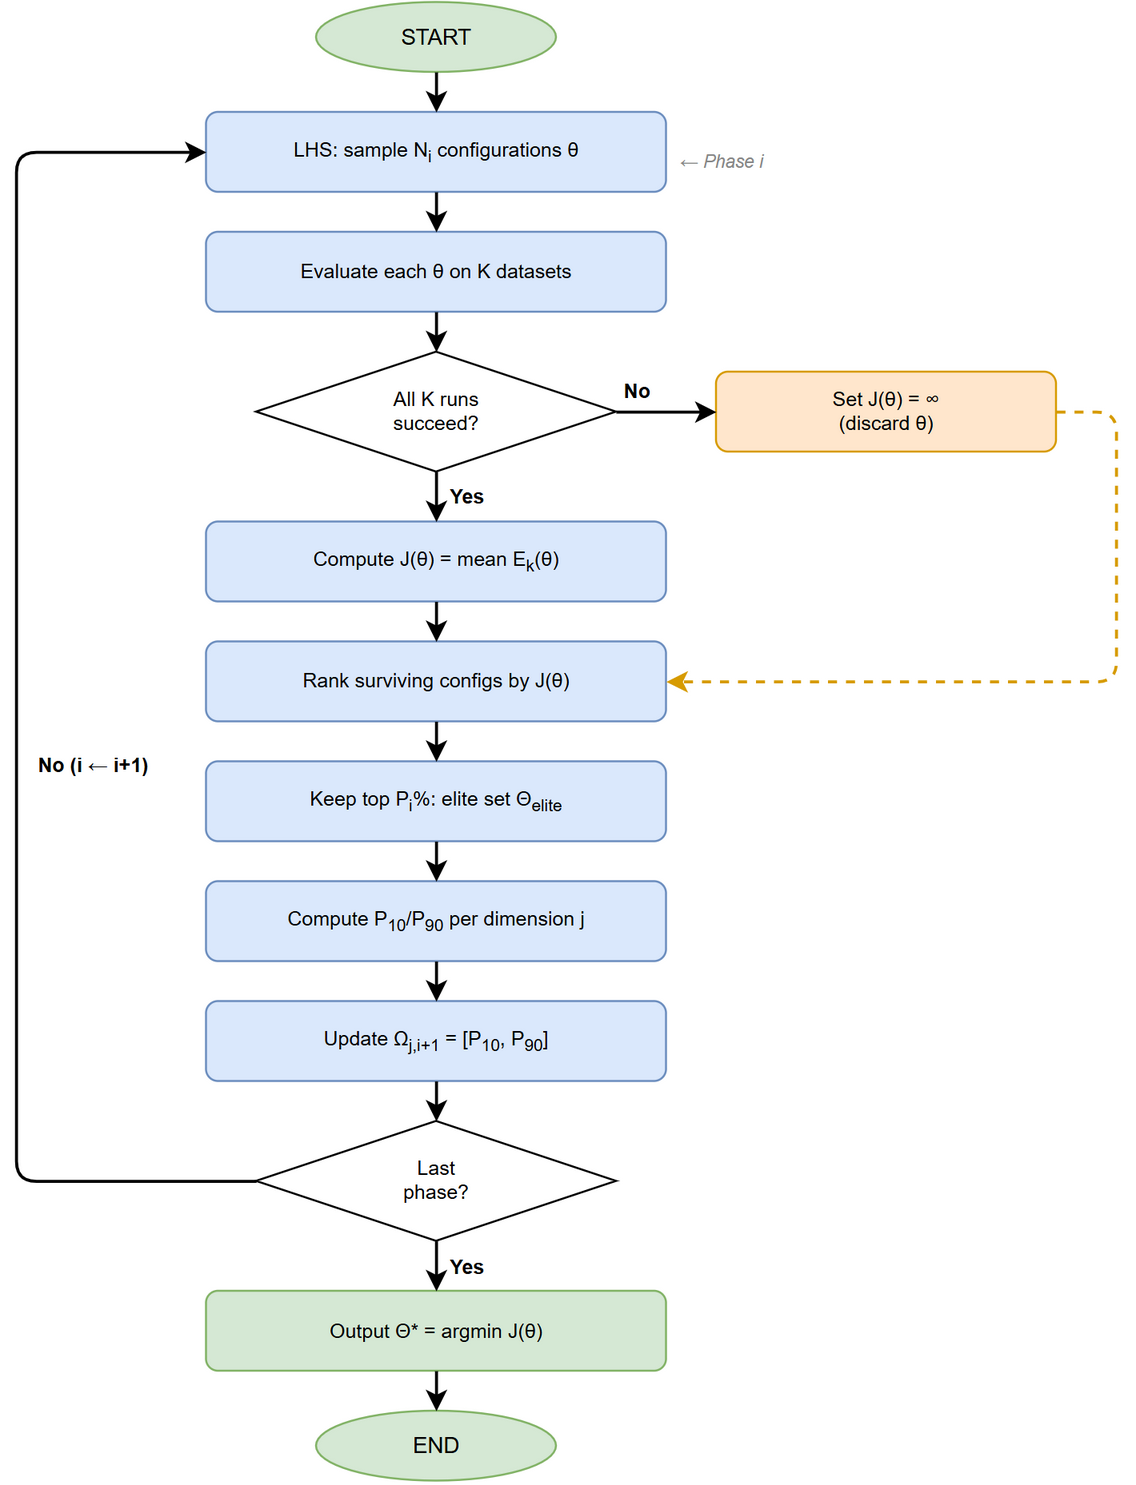
\includegraphics[width=\linewidth]{3-SLAM/3-methodology/figures/irr-flowchart}
        \caption{Algorithmic flowchart of the IRR procedure. Each phase samples $N_i$ configurations via LHS, evaluates them on $K$ datasets, discards failures (cost $= \infty$), ranks survivors by $J(\theta)$, retains the elite top $P_i\%$, and contracts the search bounds $\Omega_{j,i+1}$ using the $P_{10}$--$P_{90}$ quantile range.}
        \label{fig:irr-flowchart}
    \end{subfigure}
    \caption{IRR optimisation strategy: \subref{fig:irr-funnel}~contracting parameter search space across phases; \subref{fig:irr-flowchart}~per-phase algorithmic procedure.}
    \label{fig:irr}
\end{figure}

\subsubsection{Optimisation Metrics}

For the optimisation of the base GLIM algorithm, the cost function for candidate ranking is the Trajectory Error Percentage ($TEP$), calculated as the percentage of the ratio of Absolute Trajectory Error ($ATE$) \cite{sturmBenchmarkEvaluationRGBD2012} to the total trajectory length ($L$):
\begin{equation}
\label{eq:tep}
TEP = \frac{ATE}{L} \times 100\%.
\end{equation}
The $TEP$ effectively measures the per cent drift per metre of motion.

For the optimisation of the proposed method, the cost function is a custom metric referred to as Global Alignment and Smoothness Profile ($GASP$). This is calculated by taking the weighted sum of the $ATE$ per metre and the standard deviation of the translational Relative Pose Error ($RPE$), as defined in Equation \eqref{eq:gasp}:
\begin{equation}
\label{eq:gasp}
\text{GASP} = w_{\text{drift}} \cdot \left( \frac{ATE}{L} \right) + w_{\text{smoothness}} \cdot \text{Translational RPE}.
\end{equation}
The weights $w_{\text{drift}}$ and $w_{\text{smoothness}}$ have been empirically tuned such that each term contributes approximately equally to the total cost. Because the weighted sum mixes quantities with different units, GASP serves as a relative performance index; its values are meaningful only when compared within the same experimental framework.

\subsection{Experimental Setup}
\label{subsec:slam-experimental-setup}

The following subsection describes the datasets and evaluation protocol used to assess the methods presented above.

\subsubsection{Parameterisation Datasets}

Five datasets were used to parameterise the two optimised configurations — the refined GLIM algorithm and the proposed GNSS-augmented method. The datasets span two distinct agricultural environments: one apple orchard (Dataset~1) and four vineyard traversals (Datasets~0, 2, 3, and~4), the latter all collected at the same farm. This environmental diversity was deliberate, as including a structurally different environment reduces the risk that the parameterised configurations are over-specialised to a single terrain type.

\begin{itemize}
  \item \textbf{Dataset~0 --- Vineyard.} A forward-and-return traversal. The altitude increases gradually on the forward pass and decreases correspondingly on the return.
  \item \textbf{Dataset~1 --- Apple orchard.} A forward-and-return traversal of an apple orchard. The altitude profile is more complex than the vineyard datasets, featuring substantially more localised elevation dips and bumps throughout, making this dataset the most challenging for vertical estimation.
  \item \textbf{Dataset~2 --- Vineyard.} A single-direction traversal with no return pass, starting from the opposite end of the vineyard row relative to all other vineyard datasets. The altitude decreases gradually over the course of the traversal — the inverse of the profile observed in Datasets~0, 3, and~4.
  \item \textbf{Dataset~3 --- Vineyard.} A forward-and-return traversal at the same farm as Datasets~0, 2, and~4. The altitude profile follows the same gradual increase--decrease pattern as Datasets~0 and~4.
  \item \textbf{Dataset~4 --- Vineyard.} A forward-and-return traversal at the same farm as Datasets~0, 2, and~3, with the same altitude profile as Datasets~0 and~3.
\end{itemize}

\subsubsection{Evaluation Dataset}

The Evaluation Dataset is a held-out vineyard traversal that was not used at any stage of the parameterisation process. It was collected at the same farm as Datasets~0, 2, 3, and~4, but follows a distinct route not present in the parameterisation data. The altitude profile is consistent with that of Datasets~0, 1, 3, and~4: a gradual increase on the forward traversal and a corresponding decrease on the return. The dataset may differ from the parameterisation datasets in GNSS coverage and signal conditions, depending on the canopy density and geometry of the specific route.

The purpose of this dataset is to provide an unbiased estimate of whether the performance improvements observed during parameterisation reflect genuine algorithmic improvement, or whether they are artefacts specific to the routes on which parameters were tuned.

\subsubsection{Evaluation Protocol}

Three configurations were evaluated: the baseline GLIM algorithm, the refined GLIM algorithm with optimised parameters, and the proposed GNSS-augmented method. Each configuration was evaluated on each of the five parameterisation datasets using a single run per dataset.

For the Evaluation Dataset, each configuration was evaluated across five independent runs. This repetition is motivated by the non-deterministic behaviour of the SLAM system: internal parallelism and floating-point operation ordering cause run-to-run variation in the generated trajectory, even under identical input conditions. A single run on an unseen dataset therefore risks reporting an uncharacteristic outcome. For each metric, the mean, standard deviation, median, minimum, and maximum across the five runs are reported.

Performance is assessed using the metrics defined in \cref{sec:slam-methodology}: RMSE (per axis and aggregate 3D), ATE, maximum 3D positional error, error per metre, error percentage per metre, RPE at displacement intervals of 1\,m and 10\,m (RMSE, mean, standard deviation, and maximum translation error), and, for the proposed method, GASP.


\clearpage

\section{Results}
\label{sec:slam-results}
This section presents the empirical results from the evaluation of three localisation configurations: the baseline GLIM algorithm with default parameters, the refined GLIM algorithm with optimised parameters, and the proposed GNSS-augmented method. Each configuration was evaluated on five parameterisation datasets; additionally, all three configurations were evaluated on a held-out Evaluation Dataset, described in \cref{subsec:slam-experimental-setup}, to assess generalisation to an unseen route. Performance is reported using Root Mean Square Error (RMSE), Absolute Trajectory Error (ATE), Relative Pose Error (RPE), and, for the proposed method, the Global Alignment and Smoothness Profile (GASP) metric defined in the methodology.

\subsection{Baseline GLIM Performance}

\cref{tab:baseline_performance} reports the performance of the baseline GLIM algorithm across the five datasets. The error percentage per metre ranges from 1.253\% (Dataset~1) to 7.361\% (Dataset~2). The 3D RMSE ranges from 8.035\,m (Dataset~1) to 38.107\,m (Dataset~3), and the ATE ranges from 6.605\,m to 30.444\,m. The maximum single-point 3D error observed is 80.339\,m in Dataset~2.

\begin{table}[htbp]
\centering
\caption{Baseline GLIM performance over the five test datasets}
\label{tab:baseline_performance}
\begin{tabularx}{\textwidth}{lXXXXX}
\toprule
\textbf{Metrics} & \textbf{Dataset 0} & \textbf{Dataset 1} & \textbf{Dataset 2} & \textbf{Dataset 3} & \textbf{Dataset 4} \\ \midrule
RMSE\ x\ (m)\ & 20.776 & 7.253 & 4.097 & 4.747 & 3.598 \\
RMSE\ y\ (m)\ & 3.730 & 2.766 & 3.391 & 4.596 & 4.889 \\
RMSE\ z\ (m)\ & 15.107 & 1.747 & 35.970 & 36.908 & 25.879 \\
RMSE\ 3D\ (m)\ & 26.990 & 8.035 & 36.755 & 38.107 & 27.767 \\
ATE\ (m)\ & 19.877 & 6.605 & 25.921 & 30.444 & 25.331 \\
max\ error\ 3D\ (m)\ & 47.892 & 17.766 & 80.339 & 69.878 & 56.729 \\
error\ per\ meter\ (m)\ & 0.0340 & 0.0130 & 0.0740 & 0.0490 & 0.0420 \\
error\ percent\ per\ meter\ (\%)\ & 3.3580 & 1.2530 & 7.3610 & 4.8970 & 4.1910 \\
RPE\ 1m\ translation\ RMSE\ & 0.4697 & 0.2944 & 0.7632 & 1.0127 & 0.5356 \\
RPE\ 1m\ translation\ mean\ & 0.3100 & 0.1390 & 0.3210 & 0.3790 & 0.3170 \\
RPE\ 1m\ translation\ std\ & 0.4125 & 0.2602 & 0.6767 & 0.9384 & 0.4285 \\
RPE\ 1m\ translation\ max\ & 3.4500 & 2.8930 & 4.1800 & 15.7180 & 2.8810 \\
RPE\ 10m\ translation\ RMSE\ & 2.3790 & 1.5040 & 3.3400 & 3.3230 & 2.5920 \\
RPE\ 10m\ translation\ mean\ & 2.2680 & 1.1230 & 2.8110 & 3.0490 & 2.4040 \\
RPE\ 10m\ translation\ std\ & 0.7134 & 1.0076 & 1.8240 & 1.4120 & 0.9390 \\
RPE\ 10m\ translation\ max\ & 6.6530 & 7.9020 & 11.2070 & 16.2210 & 7.0210 \\ \bottomrule
\end{tabularx}
\end{table}

\subsection{Refined GLIM Performance}

\cref{tab:refined_performance} reports the results for the refined GLIM algorithm following parameter optimisation. The error percentage per metre ranges from 0.6081\% (Dataset~1) to 3.6150\% (Dataset~2). The 3D RMSE ranges from 3.4808\,m (Dataset~1) to 25.1789\,m (Dataset~2), and the ATE ranges from 3.2315\,m to 12.6781\,m.

\begin{table}[htbp]
\centering
\caption{Refined GLIM performance over the five datasets}
\label{tab:refined_performance}
\begin{tabularx}{\textwidth}{lXXXXX}
\toprule
\textbf{Metrics} & \textbf{Dataset 0} & \textbf{Dataset 1} & \textbf{Dataset 2} & \textbf{Dataset 3} & \textbf{Dataset 4} \\ \midrule
RMSE\ x\ (m)\ & 6.3487 & 2.5059 & 3.6146 & 3.5669 & 1.1221 \\
RMSE\ y\ (m)\ & 3.2186 & 2.3727 & 24.9149 & 3.4499 & 2.6844 \\
RMSE\ z\ (m)\ & 0.6987 & 0.4545 & 0.3994 & 1.0413 & 2.1387 \\
RMSE\ 3D\ (m)\ & 7.1522 & 3.4808 & 25.1789 & 5.0705 & 3.6110 \\
ATE\ (m)\ & 5.9190 & 3.2315 & 12.6781 & 4.6763 & 3.3144 \\
max\ error\ 3D\ (m)\ & 14.3770 & 5.5867 & 71.0506 & 13.0417 & 5.8597 \\
error\ per\ meter\ (m)\ & 0.0087 & 0.0061 & 0.0362 & 0.0075 & 0.0067 \\
error\ percent\ per\ meter\ (\%)\ & 0.8735 & 0.6081 & 3.6150 & 0.7499 & 0.6680 \\
RPE\ 1m\ translation\ RMSE\ & 0.3907 & 0.2609 & 0.5692 & 0.8317 & 0.3689 \\
RPE\ 1m\ translation\ mean\ & 0.1471 & 0.0899 & 0.3037 & 0.1133 & 0.1358 \\
RPE\ 1m\ translation\ std\ & 0.3619 & 0.2449 & 0.4814 & 0.8239 & 0.3430 \\
RPE\ 1m\ translation\ max\ & 3.1190 & 2.8235 & 2.3976 & 15.1426 & 2.7154 \\
RPE\ 10m\ translation\ RMSE\ & 1.2280 & 1.5267 & 4.6931 & 2.6912 & 1.4290 \\
RPE\ 10m\ translation\ mean\ & 0.7309 & 0.5967 & 2.6938 & 0.8912 & 0.5826 \\
RPE\ 10m\ translation\ std\ & 0.9868 & 1.4052 & 3.8430 & 2.5394 & 1.3048 \\
RPE\ 10m\ translation\ max\ & 5.7503 & 7.7271 & 10.7189 & 15.4780 & 6.6573 \\ \bottomrule
\end{tabularx}
\end{table}


\subsection{Proposed Method Performance}

\cref{tab:proposed_performance} reports the results for the proposed GNSS-augmented method. The error percentage per metre ranges from 0.0153\% (Dataset~4) to 0.0501\% (Dataset~2). The 3D RMSE ranges from 0.1097\,m (Dataset~0) to 0.2280\,m (Dataset~2), and the ATE ranges from 0.0811\,m to 0.1741\,m. The GASP metric, which combines drift rate and local pose smoothness, returned values between 0.0274 (Dataset~0) and 0.0679 (Dataset~2).

\begin{table}[htbp]
\centering
\caption{Proposed method performance over the 5 test datasets}
\label{tab:proposed_performance}
\begin{tabularx}{\textwidth}{lXXXXX}
\toprule
\textbf{Metrics} & \textbf{Dataset 0} & \textbf{Dataset 1} & \textbf{Dataset 2} & \textbf{Dataset 3} & \textbf{Dataset 4} \\ \midrule
RMSE\ x\ (m)\ & 0.0756 & 0.0528 & 0.0909 & 0.0528 & 0.0728 \\
RMSE\ y\ (m)\ & 0.0645 & 0.0906 & 0.2003 & 0.0906 & 0.0789 \\
RMSE\ z\ (m)\ & 0.0465 & 0.0347 & 0.0599 & 0.0347 & 0.0560 \\
RMSE\ 3D\ (m)\ & 0.1097 & 0.1105 & 0.2280 & 0.1105 & 0.1211 \\
ATE\ (m)\ & 0.0846 & 0.0811 & 0.1741 & 0.0811 & 0.1031 \\
max\ error\ 3D\ (m)\ & 0.7363 & 0.8963 & 1.0246 & 0.8963 & 0.7056 \\
error\ per\ meter\ (m)\ & 0.0002 & 0.0002 & 0.0005 & 0.0002 & 0.0002 \\
error\ percent\ per\ meter\ (\%)\ & 0.0171 & 0.0154 & 0.0501 & 0.0154 & 0.0153 \\
gasp & 0.0274 & 0.0290 & 0.0679 & 0.0290 & 0.0429 \\
RPE\ 1m\ translation\ RMSE\ & 0.0270 & 0.0308 & 0.0556 & 0.0308 & 0.0444 \\
RPE\ 1m\ translation\ mean\ & 0.0175 & 0.0206 & 0.0282 & 0.0206 & 0.0249 \\
RPE\ 1m\ translation\ std\ & 0.0205 & 0.0229 & 0.0479 & 0.0229 & 0.0368 \\
RPE\ 1m\ translation\ max\ & 0.2001 & 0.4906 & 0.6992 & 0.4906 & 0.6462 \\
RPE\ 10m\ translation\ RMSE\ & 0.0649 & 0.0936 & 0.1772 & 0.0936 & 0.0769 \\
RPE\ 10m\ translation\ mean\ & 0.0433 & 0.0613 & 0.0987 & 0.0613 & 0.0573 \\
RPE\ 10m\ translation\ std\ & 0.0482 & 0.0708 & 0.1471 & 0.0708 & 0.0512 \\
RPE\ 10m\ translation\ max\ & 0.3799 & 0.7620 & 0.8566 & 0.7620 & 0.5377 \\ \bottomrule
\end{tabularx}
\end{table}

\subsection{Comparative Summary}

\cref{tab:comparison_table_key_metrics} presents a side-by-side comparison of the three methods on three key metrics: error percentage per metre, RPE 1\,m translation standard deviation, and error per metre. The lowest value for each metric--dataset combination is indicated in bold.

\begin{table}[htbp]
\centering
\caption{Comparison Table of the Key Metrics (Best results in bold)}
\label{tab:comparison_table_key_metrics}
\begin{tabularx}{\textwidth}{>{\hsize=0.8\hsize}X >{\hsize=1.2\hsize}X XXXXX} % Adjusting relative widths
\toprule
\textbf{Metric} & \textbf{Method} & \textbf{Dataset 0} & \textbf{Dataset 1} & \textbf{Dataset 2} & \textbf{Dataset 3} & \textbf{Dataset 4} \\ \midrule

% Use {=} in multirow to allow text wrapping inside the X column
\multirow{3}{=}{error percent per meter (\%)} & Baseline GLIM & 3.3580 & 1.2530 & 7.3610 & 4.8970 & 4.1910 \\
 & Refined GLIM & 0.8735 & 0.6081 & 3.6150 & 0.7499 & 0.6680 \\
 & Proposed Method & \textbf{0.0171} & \textbf{0.0154} & \textbf{0.0501} & \textbf{0.0154} & \textbf{0.0153} \\ \midrule

\multirow{3}{=}{RPE 1m translation std} & Baseline GLIM & 0.4125 & 0.2602 & 0.6767 & 0.9384 & 0.4285 \\
 & Refined GLIM & 0.3619 & 0.2449 & 0.4814 & 0.8239 & 0.3430 \\
 & Proposed Method & \textbf{0.0205} & \textbf{0.0229} & \textbf{0.0479} & \textbf{0.0229} & \textbf{0.0368} \\ \midrule

\multirow{3}{=}{error per meter (m)} & Baseline GLIM & 0.0340 & 0.0130 & 0.0740 & 0.0490 & 0.0420 \\
 & Refined GLIM & 0.0087 & 0.0061 & 0.0362 & 0.0075 & 0.0067 \\
 & Proposed Method & \textbf{0.0002} & \textbf{0.0002} & \textbf{0.0005} & \textbf{0.0002} & \textbf{0.0002} \\ \bottomrule
\end{tabularx}
\end{table}

\subsection{GNSS Factor Utilisation}

\cref{tab:gnss_stats} reports the number of GNSS factors incorporated into the proposed method's factor graph relative to the total number of available GNSS measurements. Across the five datasets, the proportion of GNSS points retained after outlier rejection and incorporated as factors ranges from 0.65\% (Dataset~2) to 0.78\% (Dataset~3).

\begin{table}[htbp]
\centering
\caption{Statistics on the number of GNSS factors used for the proposed method}
\label{tab:gnss_stats}
\begin{tabularx}{\textwidth}{lXXXXX}
\toprule
\textbf{Metric} & \textbf{Dataset 0} & \textbf{Dataset 1} & \textbf{Dataset 2} & \textbf{Dataset 3} & \textbf{Dataset 4} \\ \midrule
Number of factors & 93 & 73 & 47 & 86 & 69 \\
Number of GNSS points & 13461 & 10090 & 7236 & 11071 & 9241 \\
Percent of GNSS points used & 0.69 & 0.72 & 0.65 & 0.78 & 0.75 \\ \bottomrule
\end{tabularx}
\end{table}

\subsection{Parameter Optimisation Progression}

\cref{fig:comparison_dist} shows the distribution of per-iteration errors across the four optimisation stages. \cref{fig:baseline_error_dist} plots the error percentage per metre for the baseline GLIM tuning, and \cref{fig:proposed_error_dist} plots the GASP metric for the proposed method tuning. Both plots use a logarithmic horizontal axis.

\begin{figure}[htbp]
     \centering
     % Increased width to 0.8 to make them larger now that they are stacked
     \begin{subfigure}[b]{0.8\textwidth}
         \centering
         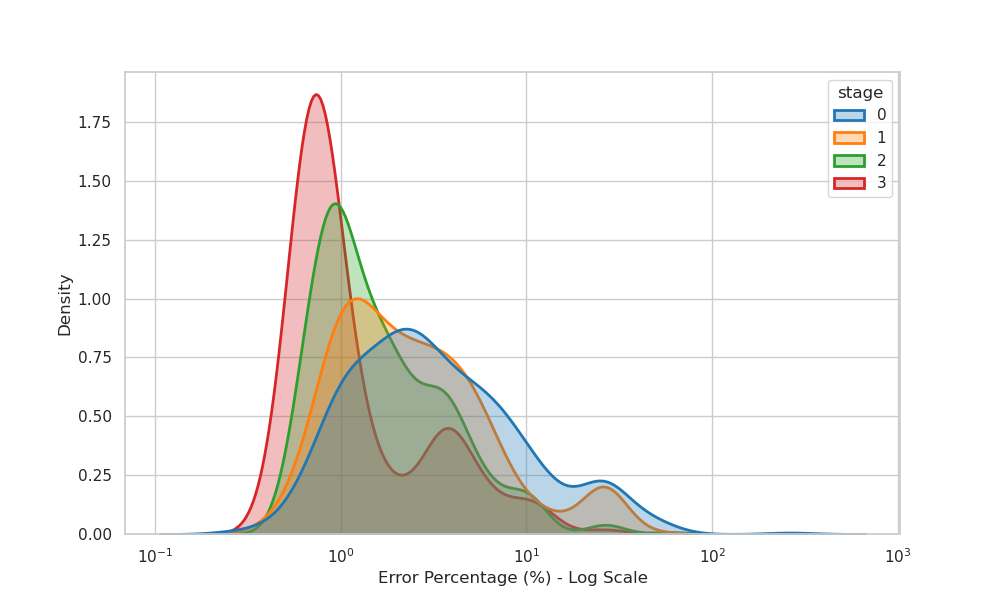
\includegraphics[width=\textwidth]{3-SLAM/3-results/figures/glim_error_distribution_by_stage_log.png}
         \caption{Baseline glim tuning.}
         \label{fig:baseline_error_dist}
     \end{subfigure}
     
     \vspace{1em} % Adds a little vertical space between the two images
     
     \begin{subfigure}[b]{0.8\textwidth}
         \centering
         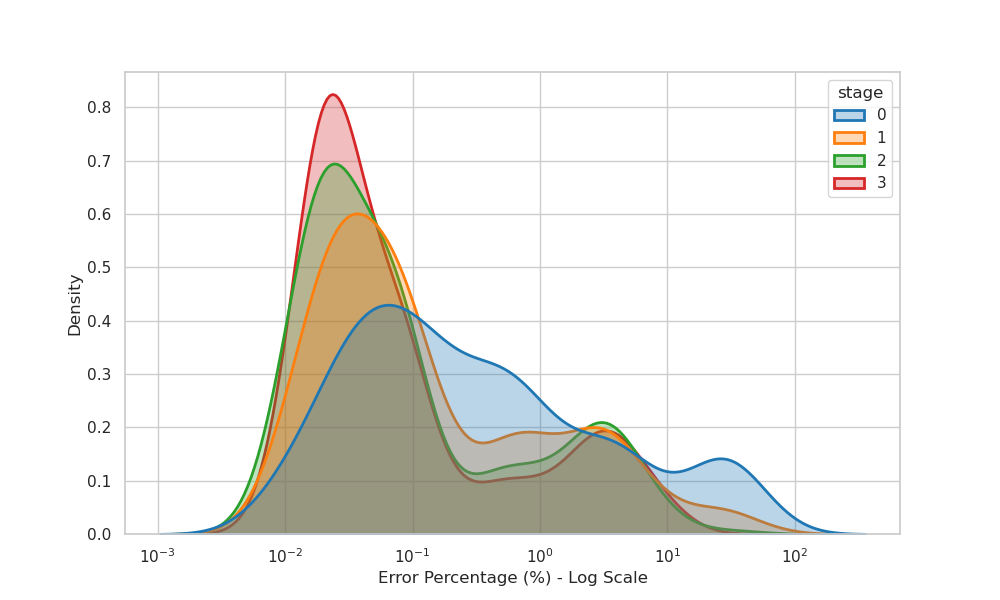
\includegraphics[width=\textwidth]{3-SLAM/3-results/figures/proposed_error_distribution_by_stage_log.png}
         \caption{Proposed method tuning.}
         \label{fig:proposed_error_dist}
     \end{subfigure}
     
     \caption{Error distribution (log scale) over optimisation stages for baseline tuning (error = error percentage) and proposed method tuning (error = GASP).}
     \label{fig:comparison_dist}
\end{figure}

\cref{fig:comparison_progression} plots the best consensus error at the end of each optimisation stage. \cref{fig:baseline_progression} tracks the error percentage for the baseline GLIM, and \cref{fig:proposed_progression} tracks the GASP metric for the proposed method. The baseline error decreases monotonically across the four stages; the proposed method's GASP score increases from stage~0 to stage~3.

\begin{figure}[htbp]
     \centering
     % Increased width from 0.48 to 0.8 for better visibility
     \begin{subfigure}[b]{0.8\textwidth}
         \centering
         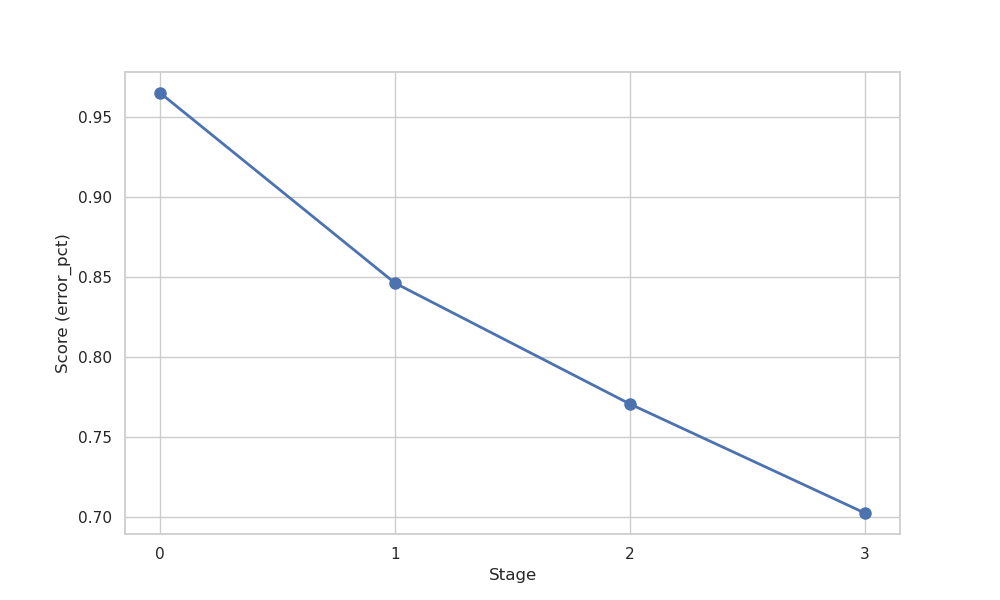
\includegraphics[width=\textwidth]{3-SLAM/3-results/figures/glim_consensus_progression.png}
         \caption{Baseline GLIM error percentage.}
         \label{fig:baseline_progression}
     \end{subfigure}

     \vspace{1.5em} % Adds vertical breathing room between the two plots

     \begin{subfigure}[b]{0.8\textwidth}
         \centering
         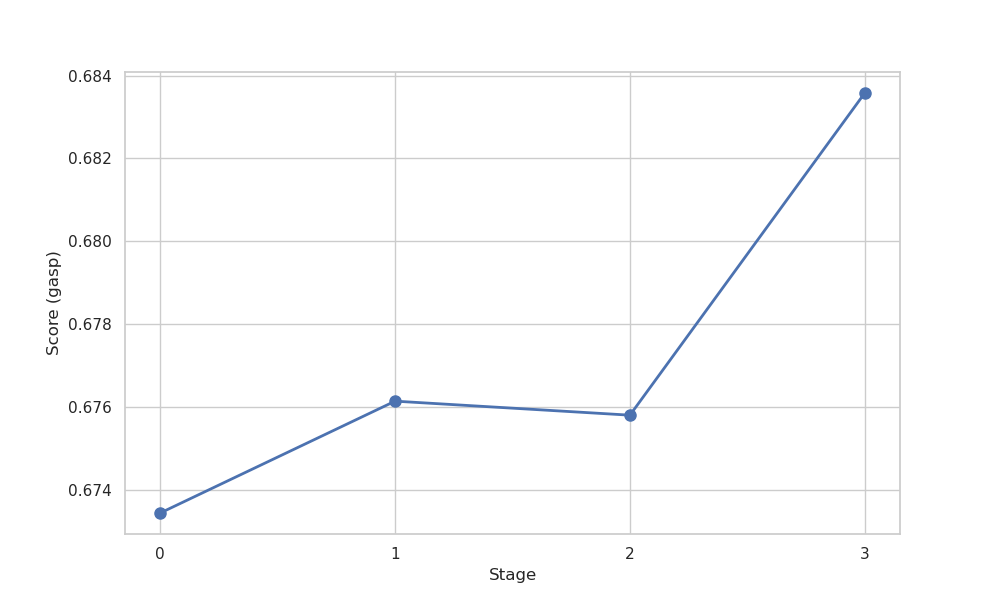
\includegraphics[width=\textwidth]{3-SLAM/3-results/figures/proposed_consensus_progression.png}
         \caption{Proposed Method GASP error.}
         \label{fig:proposed_progression}
     \end{subfigure}
     
     \caption{Consensus error over optimisation stages for baseline tuning (error = error percentage) and proposed method tuning (error = GASP).}
     \label{fig:comparison_progression}
\end{figure}

\subsection{Multi-Metric Radar Comparison}

\cref{fig:comparison_spider} presents four radar plots comparing the baseline, refined, and proposed methods across all five datasets. The four metrics displayed are error per metre, error percentage per metre, ATE, and RPE 1\,m translation standard deviation. Radial axes are plotted on a logarithmic scale.

\begin{figure}[htbp]
     \centering
     \begin{subfigure}[b]{0.48\textwidth}
         \centering
         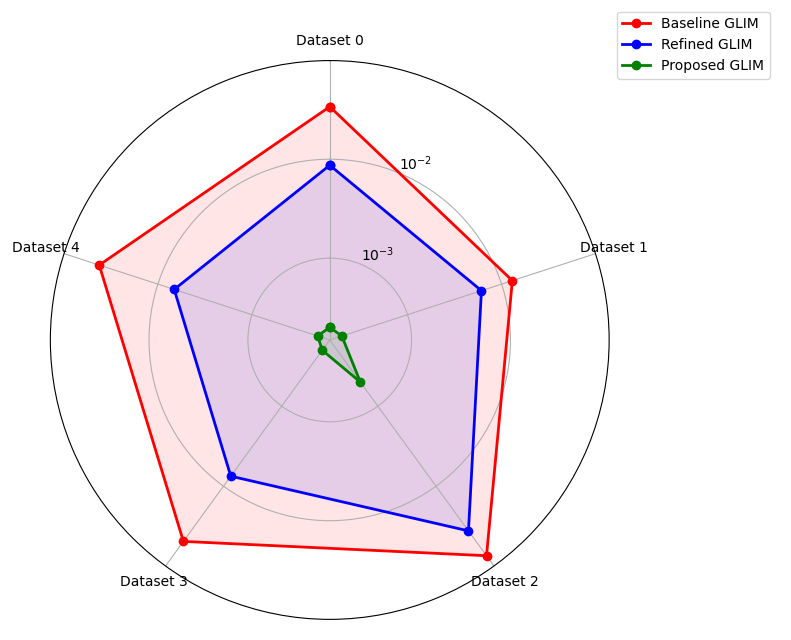
\includegraphics[width=\textwidth]{3-SLAM/3-results/figures/spider_error_per_m.png}
         \caption{Error per meter (m)}
         \label{fig:spider_epm}
     \end{subfigure}
     \hfill
     \begin{subfigure}[b]{0.48\textwidth}
         \centering
         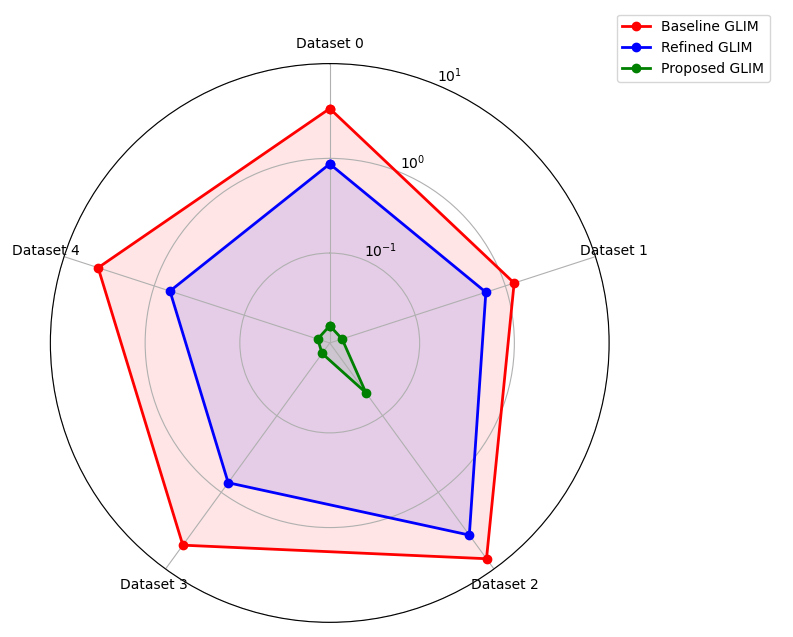
\includegraphics[width=\textwidth]{3-SLAM/3-results/figures/spider_error_pct.png}
         \caption{Error percent per meter.}
         \label{fig:spider_ep}
     \end{subfigure}
     \hfill
     \begin{subfigure}[b]{0.48\textwidth}
         \centering
         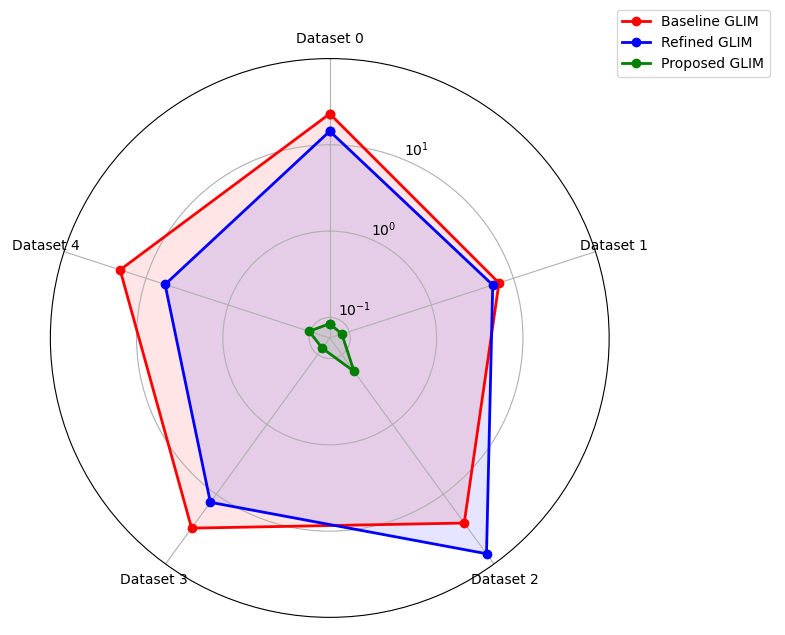
\includegraphics[width=\textwidth]{3-SLAM/3-results/figures/spider_mean_abs_pos_err.png}
         \caption{ATE error (m).}
         \label{fig:spider_ATE}
     \end{subfigure}
     \hfill
     \begin{subfigure}[b]{0.48\textwidth}
         \centering
         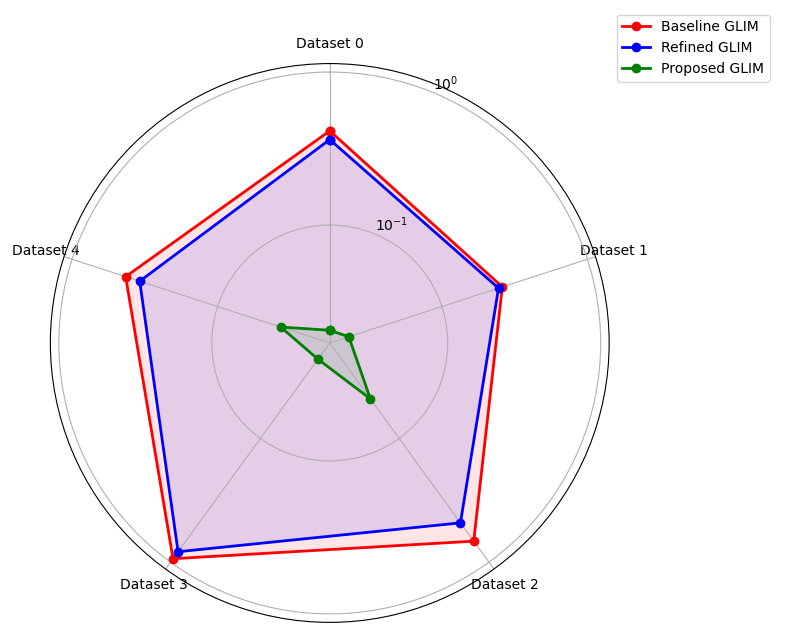
\includegraphics[width=\textwidth]{3-SLAM/3-results/figures/spider_rpe_1m_trans_std.png}
         \caption{RPE (translation only) standard deviation.} 
         \label{fig:spider_RPE_std}
     \end{subfigure}
     \caption{Spider plot comparisons of the glim baseline, refined and proposed methods for various key performance metrics.}
     \label{fig:comparison_spider}
\end{figure}

\subsection{Trajectory Visualisation}

\cref{fig:large_grid_xy} presents the planar ($x$--$y$) trajectories for each dataset. The left column shows the refined GLIM output and the right column shows the proposed method output, both plotted against the RTK~GNSS ground truth.

\begin{figure}[htbp]
    \centering
    % --- ROW 1 ---
    \begin{subfigure}[b]{0.48\textwidth}
        \centering
        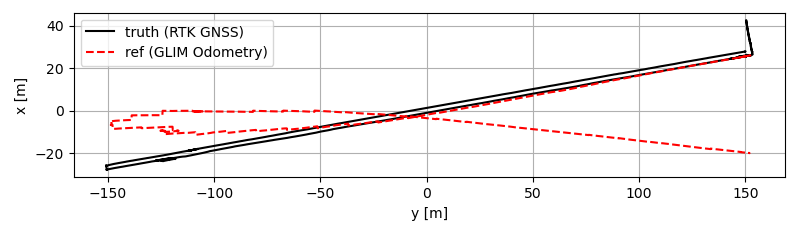
\includegraphics[width=\textwidth]{3-SLAM/3-results/figures/ds0_xy.png}
        \caption{Baseline | Dataset 0}
    \end{subfigure}
    \hfill
    \begin{subfigure}[b]{0.48\textwidth}
        \centering
        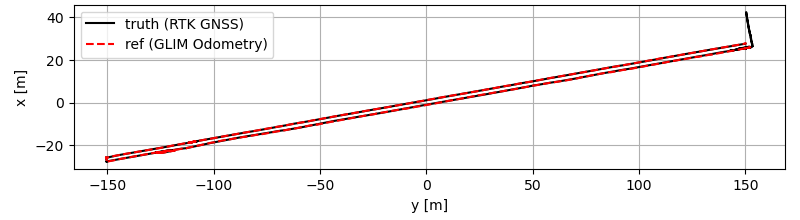
\includegraphics[width=\textwidth]{3-SLAM/3-results/figures/pds0_xy.png}
        \caption{Proposed | Dataset 0}
    \end{subfigure}

    \vspace{1em} % Vertical space between rows

    % --- ROW 2 ---
    \begin{subfigure}[b]{0.48\textwidth}
        \centering
        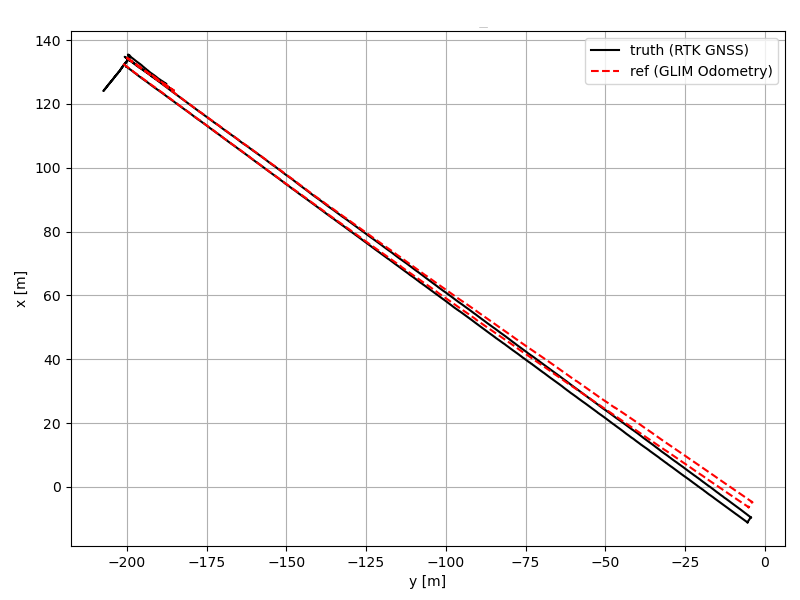
\includegraphics[width=\textwidth]{3-SLAM/3-results/figures/ds1_xy.png}
        \caption{Baseline | Dataset 1}
    \end{subfigure}
    \hfill
    \begin{subfigure}[b]{0.48\textwidth}
        \centering
        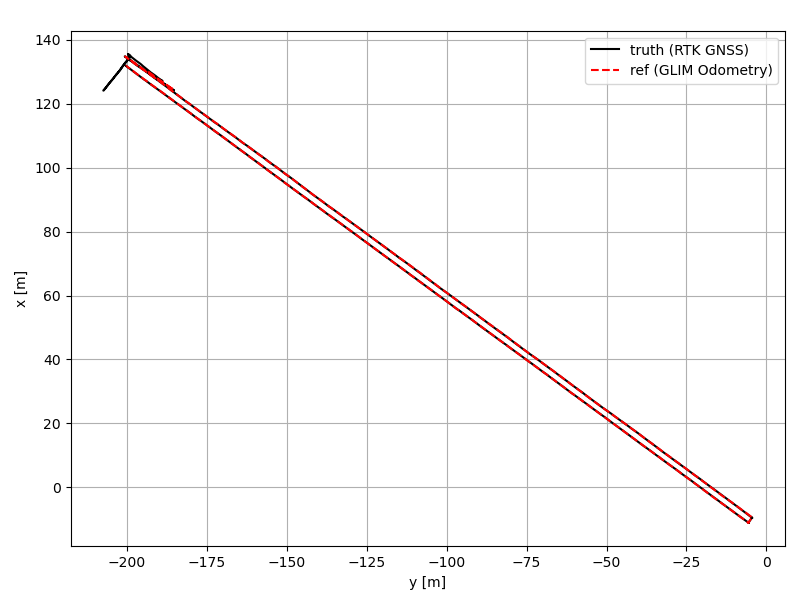
\includegraphics[width=\textwidth]{3-SLAM/3-results/figures/pds1_xy.png}
        \caption{Proposed | Dataset 1}
    \end{subfigure}

    \vspace{1em}

    % --- ROW 3 ---
    \begin{subfigure}[b]{0.48\textwidth}
        \centering
        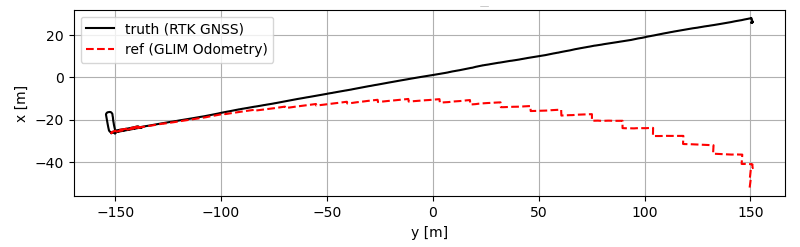
\includegraphics[width=\textwidth]{3-SLAM/3-results/figures/ds2_xy.png}
        \caption{Baseline | Dataset 2}
    \end{subfigure}
    \hfill
    \begin{subfigure}[b]{0.48\textwidth}
        \centering
        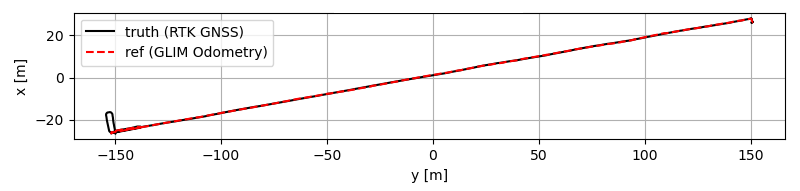
\includegraphics[width=\textwidth]{3-SLAM/3-results/figures/pds2_xy.png}
        \caption{Proposed | Dataset 2}
    \end{subfigure}

    \vspace{1em}

    % --- ROW 4 ---
    \begin{subfigure}[b]{0.48\textwidth}
        \centering
        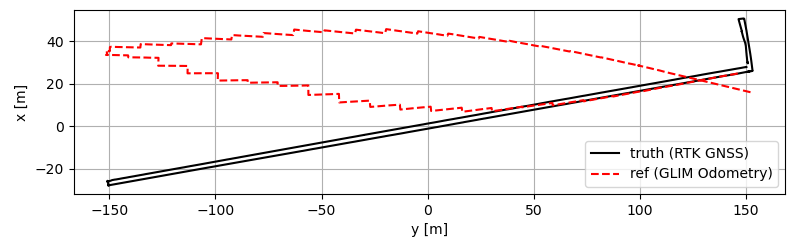
\includegraphics[width=\textwidth]{3-SLAM/3-results/figures/ds3_xy.png}
        \caption{Baseline | Dataset 3}
    \end{subfigure}
    \hfill
    \begin{subfigure}[b]{0.48\textwidth}
        \centering
        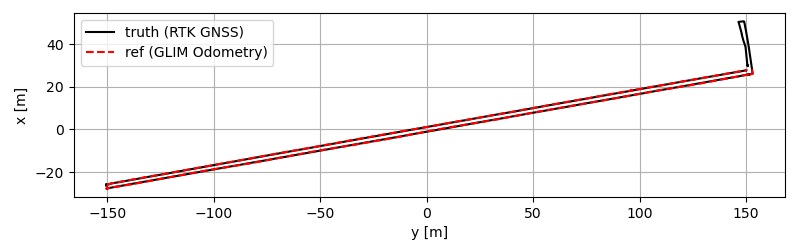
\includegraphics[width=\textwidth]{3-SLAM/3-results/figures/pds3_xy.png}
        \caption{Proposed | Dataset 3}
    \end{subfigure}

    \vspace{1em}

    % --- ROW 5 ---
    \begin{subfigure}[b]{0.48\textwidth}
        \centering
        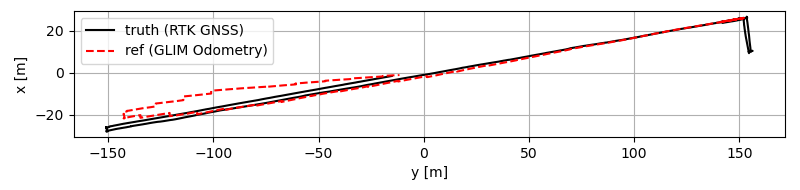
\includegraphics[width=\textwidth]{3-SLAM/3-results/figures/ds4_xy.png}
        \caption{Baseline | Dataset 4}
    \end{subfigure}
    \hfill
    \begin{subfigure}[b]{0.48\textwidth}
        \centering
        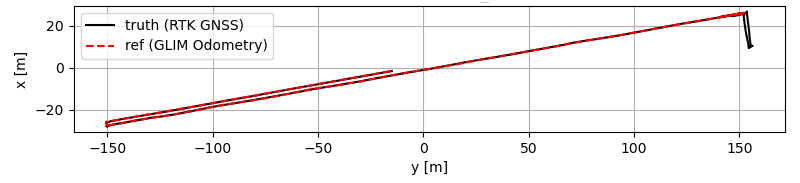
\includegraphics[width=\textwidth]{3-SLAM/3-results/figures/pds4_xy.png}
        \caption{Proposed | Dataset 4}
    \end{subfigure}

    \caption{Trajectories in XY plane from baseline GLIM and the proposed method.}
    \label{fig:large_grid_xy}
\end{figure}

\cref{fig:large_grid_z} presents the altitude ($z$-axis) trajectories for each dataset in the same layout, with the refined GLIM estimates on the left and the proposed method estimates on the right, both compared against RTK~GNSS ground truth.

\begin{figure}[htbp]
    \centering
    % --- ROW 1 ---
    \begin{subfigure}[b]{0.48\textwidth}
        \centering
        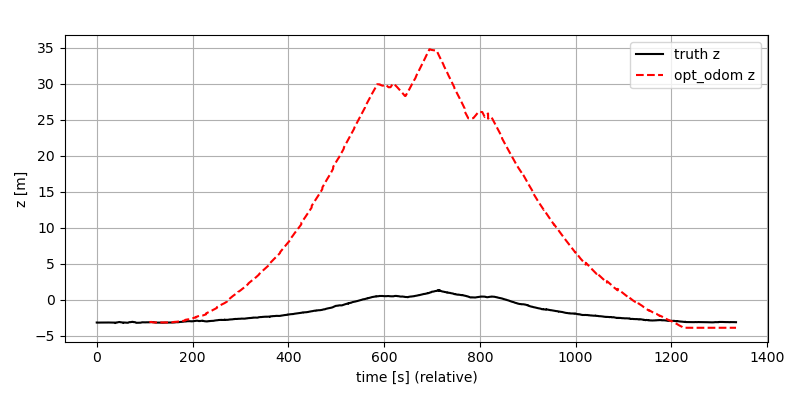
\includegraphics[width=\textwidth]{3-SLAM/3-results/figures/ds0_z.png}
        \caption{Baseline | Dataset 0}
    \end{subfigure}
    \hfill
    \begin{subfigure}[b]{0.48\textwidth}
        \centering
        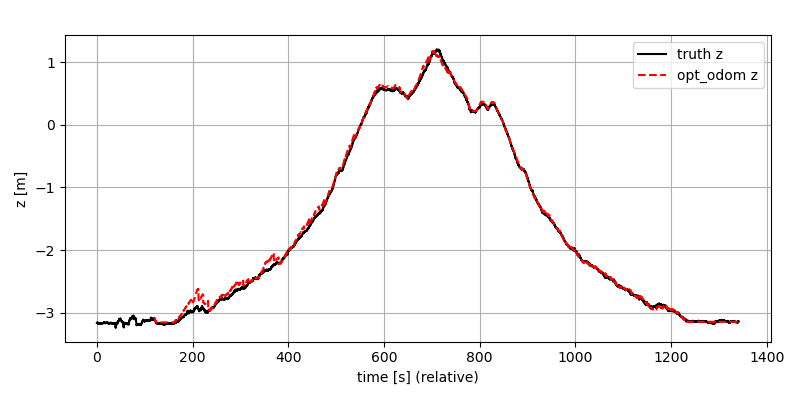
\includegraphics[width=\textwidth]{3-SLAM/3-results/figures/pds0_z.png}
        \caption{Proposed | Dataset 0}
    \end{subfigure}

    \vspace{1em} % Vertical space between rows

    % --- ROW 2 ---
    \begin{subfigure}[b]{0.48\textwidth}
        \centering
        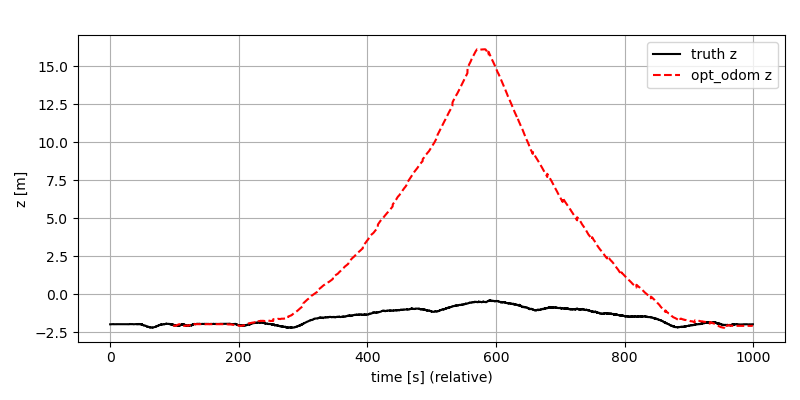
\includegraphics[width=\textwidth]{3-SLAM/3-results/figures/ds1_z.png}
        \caption{Baseline | Dataset 1}
    \end{subfigure}
    \hfill
    \begin{subfigure}[b]{0.48\textwidth}
        \centering
        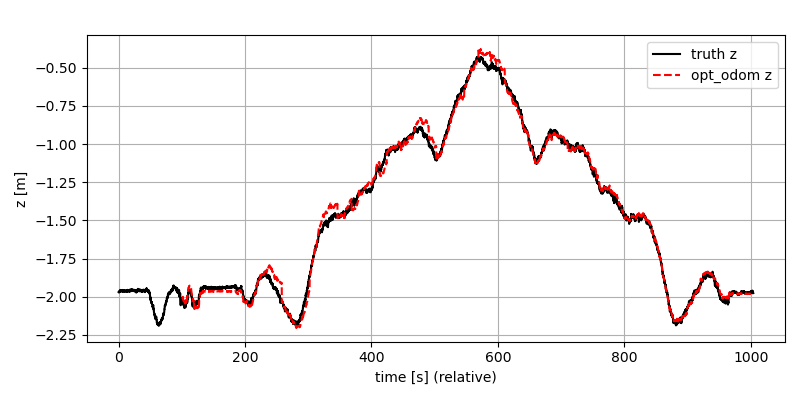
\includegraphics[width=\textwidth]{3-SLAM/3-results/figures/pds1_z.png}
        \caption{Proposed | Dataset 1}
    \end{subfigure}

    \vspace{1em}

    % --- ROW 3 ---
    \begin{subfigure}[b]{0.48\textwidth}
        \centering
        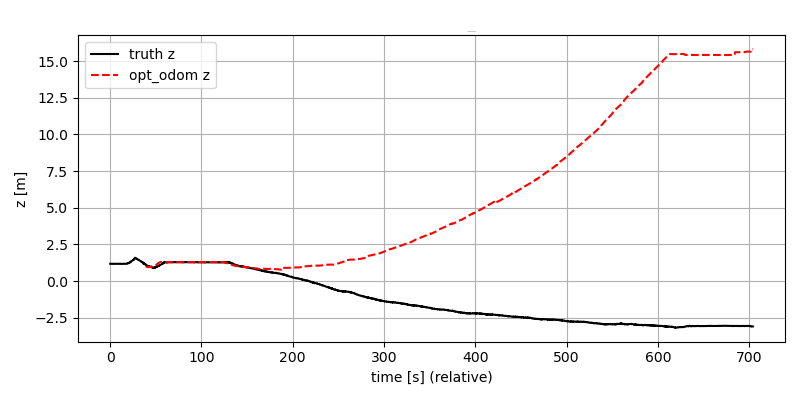
\includegraphics[width=\textwidth]{3-SLAM/3-results/figures/ds2_z.png}
        \caption{Baseline | Dataset 2}
    \end{subfigure}
    \hfill
    \begin{subfigure}[b]{0.48\textwidth}
        \centering
        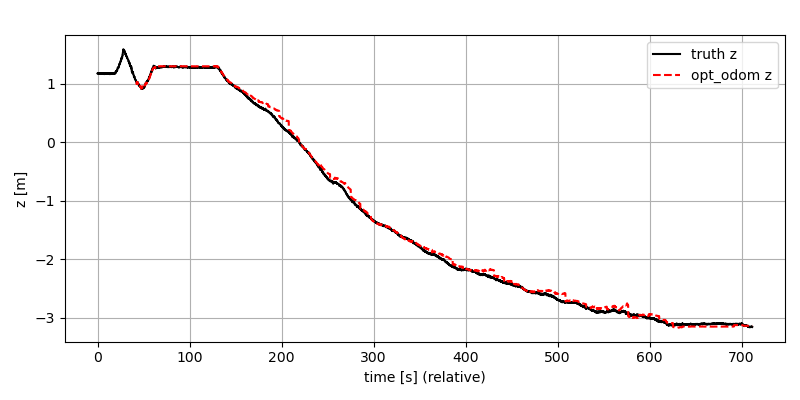
\includegraphics[width=\textwidth]{3-SLAM/3-results/figures/pds2_z.png}
        \caption{Proposed | Dataset 2}
    \end{subfigure}

    \vspace{1em}

    % --- ROW 4 ---
    \begin{subfigure}[b]{0.48\textwidth}
        \centering
        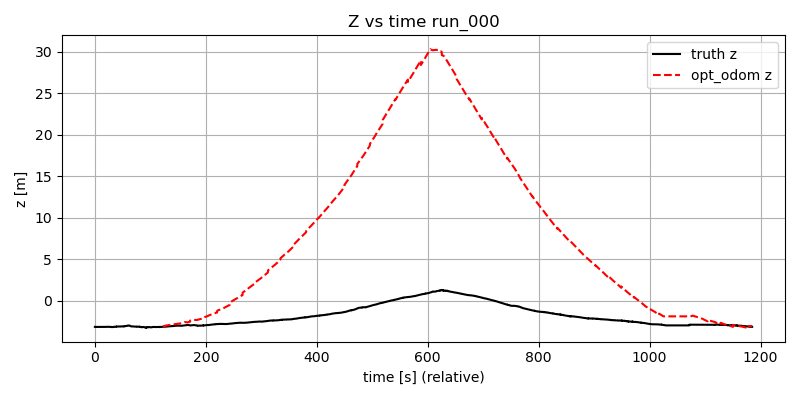
\includegraphics[width=\textwidth]{3-SLAM/3-results/figures/ds3_z.png}
        \caption{Baseline | Dataset 3}
    \end{subfigure}
    \hfill
    \begin{subfigure}[b]{0.48\textwidth}
        \centering
        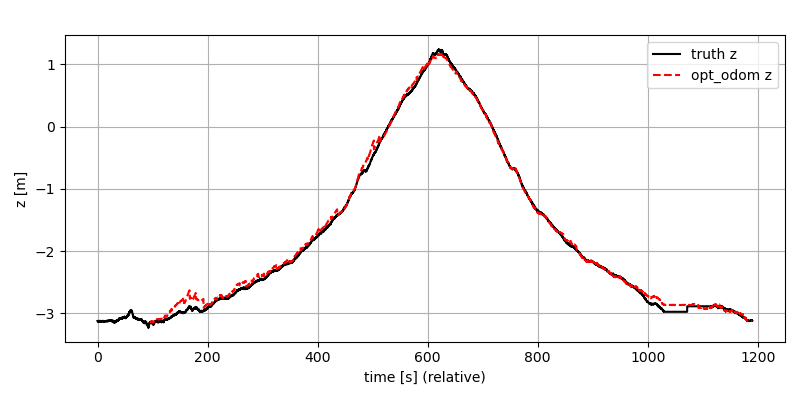
\includegraphics[width=\textwidth]{3-SLAM/3-results/figures/pds3_z.png}
        \caption{Proposed | Dataset 3}
    \end{subfigure}

    \vspace{1em}

    % --- ROW 5 ---
    \begin{subfigure}[b]{0.48\textwidth}
        \centering
        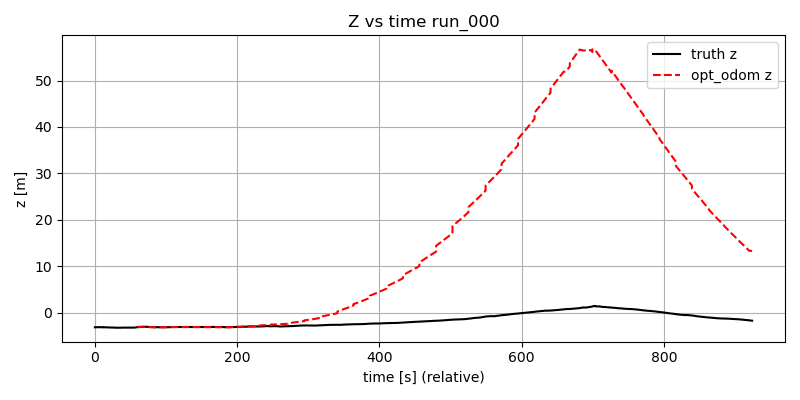
\includegraphics[width=\textwidth]{3-SLAM/3-results/figures/ds4_z.png}
        \caption{Baseline | Dataset 4}
    \end{subfigure}
    \hfill
    \begin{subfigure}[b]{0.48\textwidth}
        \centering
        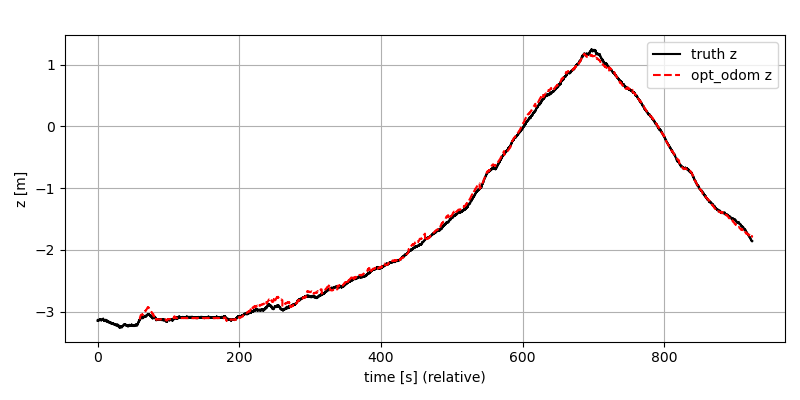
\includegraphics[width=\textwidth]{3-SLAM/3-results/figures/pds4_z.png}
        \caption{Proposed | Dataset 4}
    \end{subfigure}

    \caption{Trajectories in Z plane from baseline GLIM and the proposed method.}
    \label{fig:large_grid_z}
\end{figure}

\subsection{Evaluation Dataset Results}
\label{subsec:slam-eval-results}

The following subsections report performance on the held-out Evaluation Dataset as described in \cref{subsec:slam-experimental-setup}. Each configuration was evaluated across five independent runs; each table cell reports the aggregate statistic over those runs (mean, standard deviation, median, minimum, and maximum). This structure differs from the parameterisation dataset tables above, which report a single run per dataset.

\subsubsection{Baseline GLIM --- Evaluation Dataset}

\cref{tab:eval_baseline_performance} reports the baseline GLIM performance on the Evaluation Dataset. The mean error percentage per metre is 1.9612\% (std 0.4519\%), which falls within the range observed across the five parameterisation datasets (1.253\%--7.361\%). The mean RMSE 3D is 17.4799\,m and the mean ATE is 13.3863\,m, with the trajectory length averaging approximately 682\,m across the five runs.

\begin{table}[htbp]
\centering
\caption{Baseline GLIM performance on the Evaluation Dataset (mean, std, median, min, and max across five independent runs)}
\label{tab:eval_baseline_performance}
\begin{tabularx}{\textwidth}{lXXXXX}
\toprule
\textbf{Metrics} & \textbf{Mean} & \textbf{Std} & \textbf{Median} & \textbf{Min} & \textbf{Max} \\ \midrule
RMSE\ x\ (m)\        & 8.5597  & 5.6389 & 9.2456  & 2.1927  & 16.9319 \\
RMSE\ y\ (m)\        & 1.0545  & 0.5029 & 1.2180  & 0.2744  & 1.6128  \\
RMSE\ z\ (m)\        & 14.5590 & 2.2620 & 14.2411 & 11.9558 & 18.1913 \\
RMSE\ 3D\ (m)\       & 17.4799 & 3.6283 & 17.0259 & 12.2617 & 22.2915 \\
ATE\ (m)\            & 13.3863 & 3.1436 & 13.5756 & 9.1031  & 17.9034 \\
max\ error\ 3D\ (m)\ & 35.4544 & 6.6132 & 35.7962 & 24.9744 & 42.6418 \\
error\ per\ meter\ (m)\        & 0.0196  & 0.0045 & 0.0198  & 0.0134  & 0.0261  \\
error\ percent\ per\ meter\ (\%)\ & 1.9612  & 0.4519 & 1.9785  & 1.3390  & 2.6050  \\
RPE\ 1m\ translation\ RMSE\  & 0.1153 & 0.0649 & 0.1008 & 0.0466 & 0.2178 \\
RPE\ 1m\ translation\ mean\  & 0.0350 & 0.0080 & 0.0332 & 0.0253 & 0.0469 \\
RPE\ 1m\ translation\ std\   & 0.1093 & 0.0657 & 0.0952 & 0.0391 & 0.2127 \\
RPE\ 1m\ translation\ max\   & 1.6539 & 1.0152 & 1.4059 & 0.5472 & 3.2732 \\
RPE\ 10m\ translation\ RMSE\ & 0.1840 & 0.1104 & 0.1350 & 0.1202 & 0.3804 \\
RPE\ 10m\ translation\ mean\ & 0.0829 & 0.0354 & 0.0684 & 0.0640 & 0.1460 \\
RPE\ 10m\ translation\ std\  & 0.1638 & 0.1055 & 0.1163 & 0.1017 & 0.3513 \\
RPE\ 10m\ translation\ max\  & 1.8315 & 1.2155 & 1.3836 & 1.0030 & 3.9561 \\ \bottomrule
\end{tabularx}
\end{table}

\subsubsection{Refined GLIM --- Evaluation Dataset}

\cref{tab:eval_refined_performance} reports the refined GLIM performance on the Evaluation Dataset. The mean error percentage per metre is 0.6215\% (std 0.1089\%), consistent with the parameterisation dataset range of 0.608\%--3.615\%. However, the maximum 3D positional error exhibits a mean of 39.5938\,m with a standard deviation of 60.9811\,m and a maximum of 148.6057\,m, against a median of only 13.0861\,m. This large discrepancy between mean and median indicates that at least one run experienced a catastrophic failure, with the median providing a more representative estimate of typical performance. The same instability is evident in the RPE metrics, where the mean and standard deviation are far in excess of the corresponding median values.

\begin{table}[htbp]
\centering
\caption{Refined GLIM performance on the Evaluation Dataset (mean, std, median, min, and max across five independent runs). The high standard deviation on max error 3D, RPE 1\,m RMSE/std, and RPE 10\,m RMSE/std indicates that at least one run experienced a catastrophic localisation failure; median values are more representative of typical performance.}
\label{tab:eval_refined_performance}
\begin{tabularx}{\textwidth}{lXXXXX}
\toprule
\textbf{Metrics} & \textbf{Mean} & \textbf{Std} & \textbf{Median} & \textbf{Min} & \textbf{Max} \\ \midrule
RMSE\ x\ (m)\        & 5.5597  & 1.0624  & 5.6697  & 3.8536 & 6.7263   \\
RMSE\ y\ (m)\        & 1.6605  & 0.6931  & 1.3737  & 1.1688 & 2.8703   \\
RMSE\ z\ (m)\        & 0.8144  & 0.2925  & 0.8298  & 0.3895 & 1.2087   \\
RMSE\ 3D\ (m)\       & 5.8987  & 1.0561  & 6.2477  & 4.1607 & 6.9222   \\
ATE\ (m)\            & 4.3123  & 0.7479  & 4.4489  & 3.0535 & 4.9758   \\
max\ error\ 3D\ (m)\ & 39.5938 & 60.9811 & 13.0861 & 9.1552 & 148.6057 \\
error\ per\ meter\ (m)\        & 0.0062 & 0.0011 & 0.0065 & 0.0045 & 0.0072 \\
error\ percent\ per\ meter\ (\%)\ & 0.6215 & 0.1089 & 0.6501 & 0.4453 & 0.7192 \\
RPE\ 1m\ translation\ RMSE\  & 0.4082  & 0.8182  & 0.0443  & 0.0353 & 1.8718   \\
RPE\ 1m\ translation\ mean\  & 0.0301  & 0.0129  & 0.0249  & 0.0225 & 0.0531   \\
RPE\ 1m\ translation\ std\   & 0.4019  & 0.8213  & 0.0367  & 0.0272 & 1.8711   \\
RPE\ 1m\ translation\ max\   & 30.2296 & 66.2890 & 0.5803  & 0.5403 & 148.8110 \\
RPE\ 10m\ translation\ RMSE\ & 0.4625  & 0.8266  & 0.0864  & 0.0662 & 1.9405   \\
RPE\ 10m\ translation\ mean\ & 0.0591  & 0.0121  & 0.0534  & 0.0462 & 0.0766   \\
RPE\ 10m\ translation\ std\  & 0.4475  & 0.8342  & 0.0679  & 0.0474 & 1.9390   \\
RPE\ 10m\ translation\ max\  & 30.3526 & 66.1113 & 0.8106  & 0.5282 & 148.6158 \\ \bottomrule
\end{tabularx}
\end{table}

\subsubsection{Proposed Method --- Evaluation Dataset}

\cref{tab:eval_proposed_performance} reports the proposed method's performance on the Evaluation Dataset. The mean error percentage per metre is 0.0166\% with a standard deviation of 0.0004\%, indicating highly consistent performance across all five runs. The mean RMSE 3D is 0.1459\,m and the mean ATE is 0.1135\,m. The GASP metric has a mean of 0.0508 (std 0.0081), which is consistent with the range observed on the parameterisation datasets (0.0274--0.0679).

\begin{table}[htbp]
\centering
\caption{Proposed method performance on the Evaluation Dataset (mean, std, median, min, and max across five independent runs)}
\label{tab:eval_proposed_performance}
\begin{tabularx}{\textwidth}{lXXXXX}
\toprule
\textbf{Metrics} & \textbf{Mean} & \textbf{Std} & \textbf{Median} & \textbf{Min} & \textbf{Max} \\ \midrule
RMSE\ x\ (m)\        & 0.0958   & 0.0091   & 0.0949   & 0.0842   & 0.1070   \\
RMSE\ y\ (m)\        & 0.1010   & 0.0117   & 0.1067   & 0.0803   & 0.1074   \\
RMSE\ z\ (m)\        & 0.0426   & 0.0046   & 0.0433   & 0.0369   & 0.0493   \\
RMSE\ 3D\ (m)\       & 0.1459   & 0.0113   & 0.1493   & 0.1264   & 0.1535   \\
ATE\ (m)\            & 0.1135   & 0.0027   & 0.1131   & 0.1112   & 0.1179   \\
max\ error\ 3D\ (m)\ & 0.8573   & 0.1265   & 0.8569   & 0.6631   & 0.9732   \\
error\ per\ meter\ (m)\        & 0.000166 & 0.0000035& 0.000165 & 0.000163 & 0.000172 \\
error\ percent\ per\ meter\ (\%)\ & 0.0166   & 0.0004   & 0.0165   & 0.0163   & 0.0172   \\
GASP\                & 0.0508   & 0.0081   & 0.0520   & 0.0385   & 0.0607   \\
RPE\ 1m\ translation\ RMSE\  & 0.0526 & 0.0076 & 0.0542 & 0.0412 & 0.0620 \\
RPE\ 1m\ translation\ mean\  & 0.0284 & 0.0019 & 0.0287 & 0.0260 & 0.0307 \\
RPE\ 1m\ translation\ std\   & 0.0441 & 0.0080 & 0.0454 & 0.0319 & 0.0539 \\
RPE\ 1m\ translation\ max\   & 0.6703 & 0.1050 & 0.6443 & 0.5714 & 0.8132 \\
RPE\ 10m\ translation\ RMSE\ & 0.1120 & 0.0204 & 0.1048 & 0.0868 & 0.1355 \\
RPE\ 10m\ translation\ mean\ & 0.0729 & 0.0028 & 0.0739 & 0.0682 & 0.0755 \\
RPE\ 10m\ translation\ std\  & 0.0841 & 0.0251 & 0.0759 & 0.0536 & 0.1132 \\
RPE\ 10m\ translation\ max\  & 0.7674 & 0.2078 & 0.7978 & 0.5085 & 0.9709 \\ \bottomrule
\end{tabularx}
\end{table}

\subsubsection{Evaluation Dataset Comparative Summary}

\cref{tab:eval_comparison_key_metrics} presents a side-by-side comparison of the three methods on three key metrics across the Evaluation Dataset. The proposed method achieves the lowest mean value for all three metrics. The refined GLIM's mean RPE 1\,m translation standard deviation exceeds that of the baseline due to the contribution of the catastrophic failure run; the median values for this metric restore the expected baseline--refined--proposed ordering.

\begin{table}[htbp]
\centering
\caption{Comparison of key metrics on the Evaluation Dataset (mean, std, and median across five independent runs; best mean per row in bold)}
\label{tab:eval_comparison_key_metrics}
\begin{tabularx}{\textwidth}{>{\hsize=0.8\hsize}X >{\hsize=1.2\hsize}X X X X}
\toprule
\textbf{Metrics} & \textbf{Method} & \textbf{Mean} & \textbf{Std} & \textbf{Median} \\ \midrule

\multirow{3}{=}{error percent per meter (\%)}
 & Baseline GLIM  & 1.9612 & 0.4519 & 1.9785 \\
 & Refined GLIM   & 0.6215 & 0.1089 & 0.6501 \\
 & Proposed Method & \textbf{0.0166} & 0.0004 & 0.0165 \\ \midrule

\multirow{3}{=}{RPE 1m translation std}
 & Baseline GLIM  & 0.1093 & 0.0657 & 0.0952 \\
 & Refined GLIM   & 0.4019 & 0.8213 & 0.0367 \\
 & Proposed Method & \textbf{0.0441} & 0.0080 & 0.0454 \\ \midrule

\multirow{3}{=}{error per meter (m)}
 & Baseline GLIM  & 0.0196   & 0.0045    & 0.0198   \\
 & Refined GLIM   & 0.0062   & 0.0011    & 0.0065   \\
 & Proposed Method & \textbf{0.000166} & 0.0000035 & 0.000165 \\ \bottomrule

\end{tabularx}
\end{table}

\clearpage

\section{Discussion}
\label{sec:slam-discussion}


\subsection{Baseline GLIM Performance Analysis}

The evaluation of the baseline GLIM algorithm revealed two critical failure modes that fundamentally compromised the reliability of its localisation: systematic vertical drift and a catastrophic ``point of no return'' in planar estimation. \cref{tab:baseline_performance} reports the quantitative performance across all datasets.

\subsubsection{Vertical Drift}
The baseline algorithm exhibited systematic drift in the positive altitude ($z$-axis) direction. This drift is illustrated in Dataset 4 (\cref{fig:ds4_z_baseline}), where the vehicle drives a linear trajectory down a vineyard row. Although the actual environment features an elevation gain of approximately 5~m, the baseline GLIM algorithm accumulated nearly 30~m of vertical drift by the end of the row.

This drift demonstrated a self-correcting phenomenon during the return traversal. As the vehicle returned in the opposite direction, the vertical error decreased at a rate symmetrical to its initial accumulation, eventually converging back to the ground truth trajectory at the start of the row. This behaviour suggests that the initial drift was effectively encoded into the generated LiDAR map. During the return pass, the scan-matching process was constrained by this previously mapped geometry. Consequently, the odometry ``undid'' the accumulated drift by aligning the current scans with the erroneous elevation of the existing map. 

This vertical distortion of the map did not appear to hinder subsequent scan matching or loop closure. The algorithm remained capable of registering scans against a map with smooth but substantial Z-axis distortion. This resilience may be a byproduct of the specific environment, characterised by repetitive A-B linear paths with minimal lateral movement—which allows the scan matcher to maintain strong geometric overlap in the X-Y plane despite vertical inconsistencies.

\subsubsection{Planar Drift}
In contrast to the recoverable nature of vertical drift, errors in the X-Y plane frequently led to catastrophic, irrecoverable failure. This ``point of no return'' is most evident in \cref{fig:ds0_xy_baseline}, where the baseline algorithm maintains high accuracy for the first half of the traversal before experiencing a sudden, exponential increase in error. 

At this threshold, the accumulated planar drift distorts the LiDAR map to such an extent that subsequent scan matching becomes unreliable. After this occurs, the trajectory becomes increasingly jagged and stochastic, likely caused by false-positive scan matches that introduce large, discontinuous jumps in the pose estimation and map structure. 

This failure mode is particularly prevalent in the structured and repetitive environments of vineyard rows. Small angular or lateral drifts cause parallel rows in the LiDAR map to diverge or overlap incorrectly. Once this map distortion exceeds the scan matcher's convergence radius, the algorithm may incorrectly register the vehicle's current scan against an adjacent row. This ``row-skipping'' effect creates a feedback loop of map corruption, where each incorrect match further distorts the global map, making recovery unlikely for the remainder of the trajectory, as illustrated in \cref{fig:row-skip-baseline}.

\begin{figure}[htbp]
    \centering
    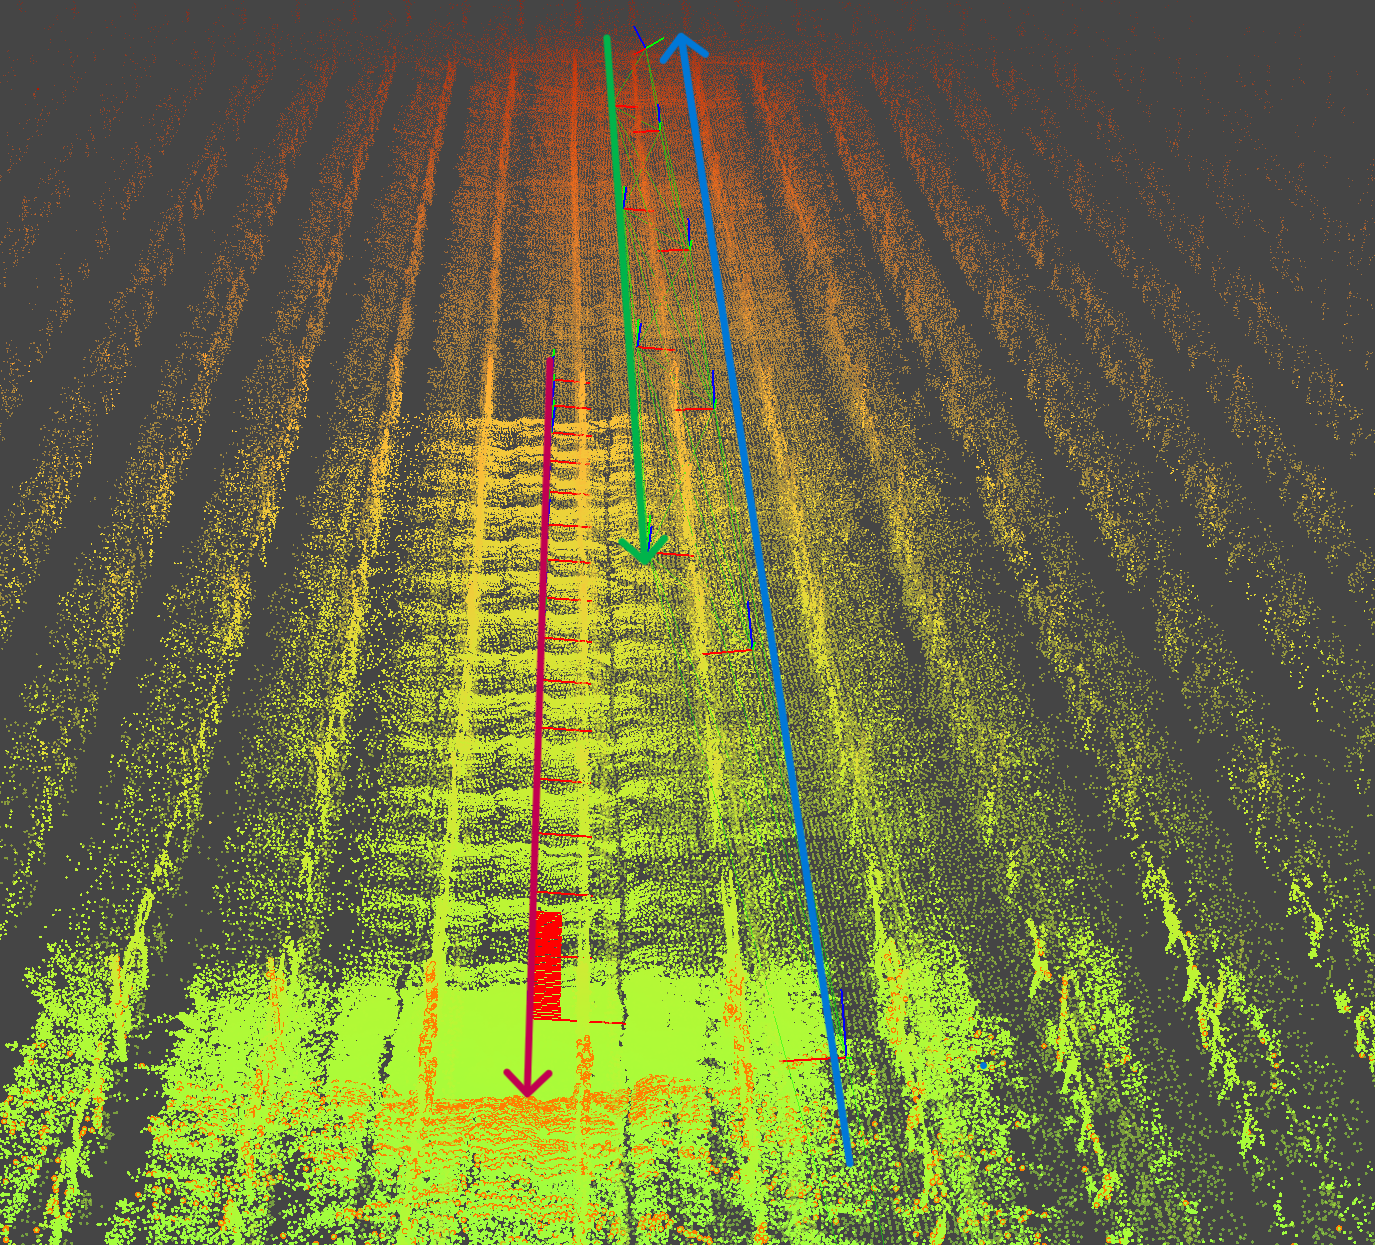
\includegraphics[width=0.85\linewidth]{3-SLAM/3-discussion/figures/row_jump.png}
    \caption{Row-skipping failure exhibited by the baseline GLIM SLAM. The blue arrow (right) shows the robot trajectory up the row. The green arrow (centre) shows the correct return traversal down the adjacent row. Approximately mid-row, the estimated trajectory abruptly shifts one lane to the left (red arrow), where scan matching has falsely converged against the geometry of the neighbouring row.}
    \label{fig:row-skip-baseline}
\end{figure}

The inherent self-similarity driving this failure is visible in the raw LiDAR map: as shown in \cref{fig:zoomedRowsSLAMMap}, the vineyard rows are geometrically indistinguishable from one another, confirming that the corridor-like structure provides no longitudinal discriminability for the scan matcher.

\begin{figure}[htbp]
    \centering
    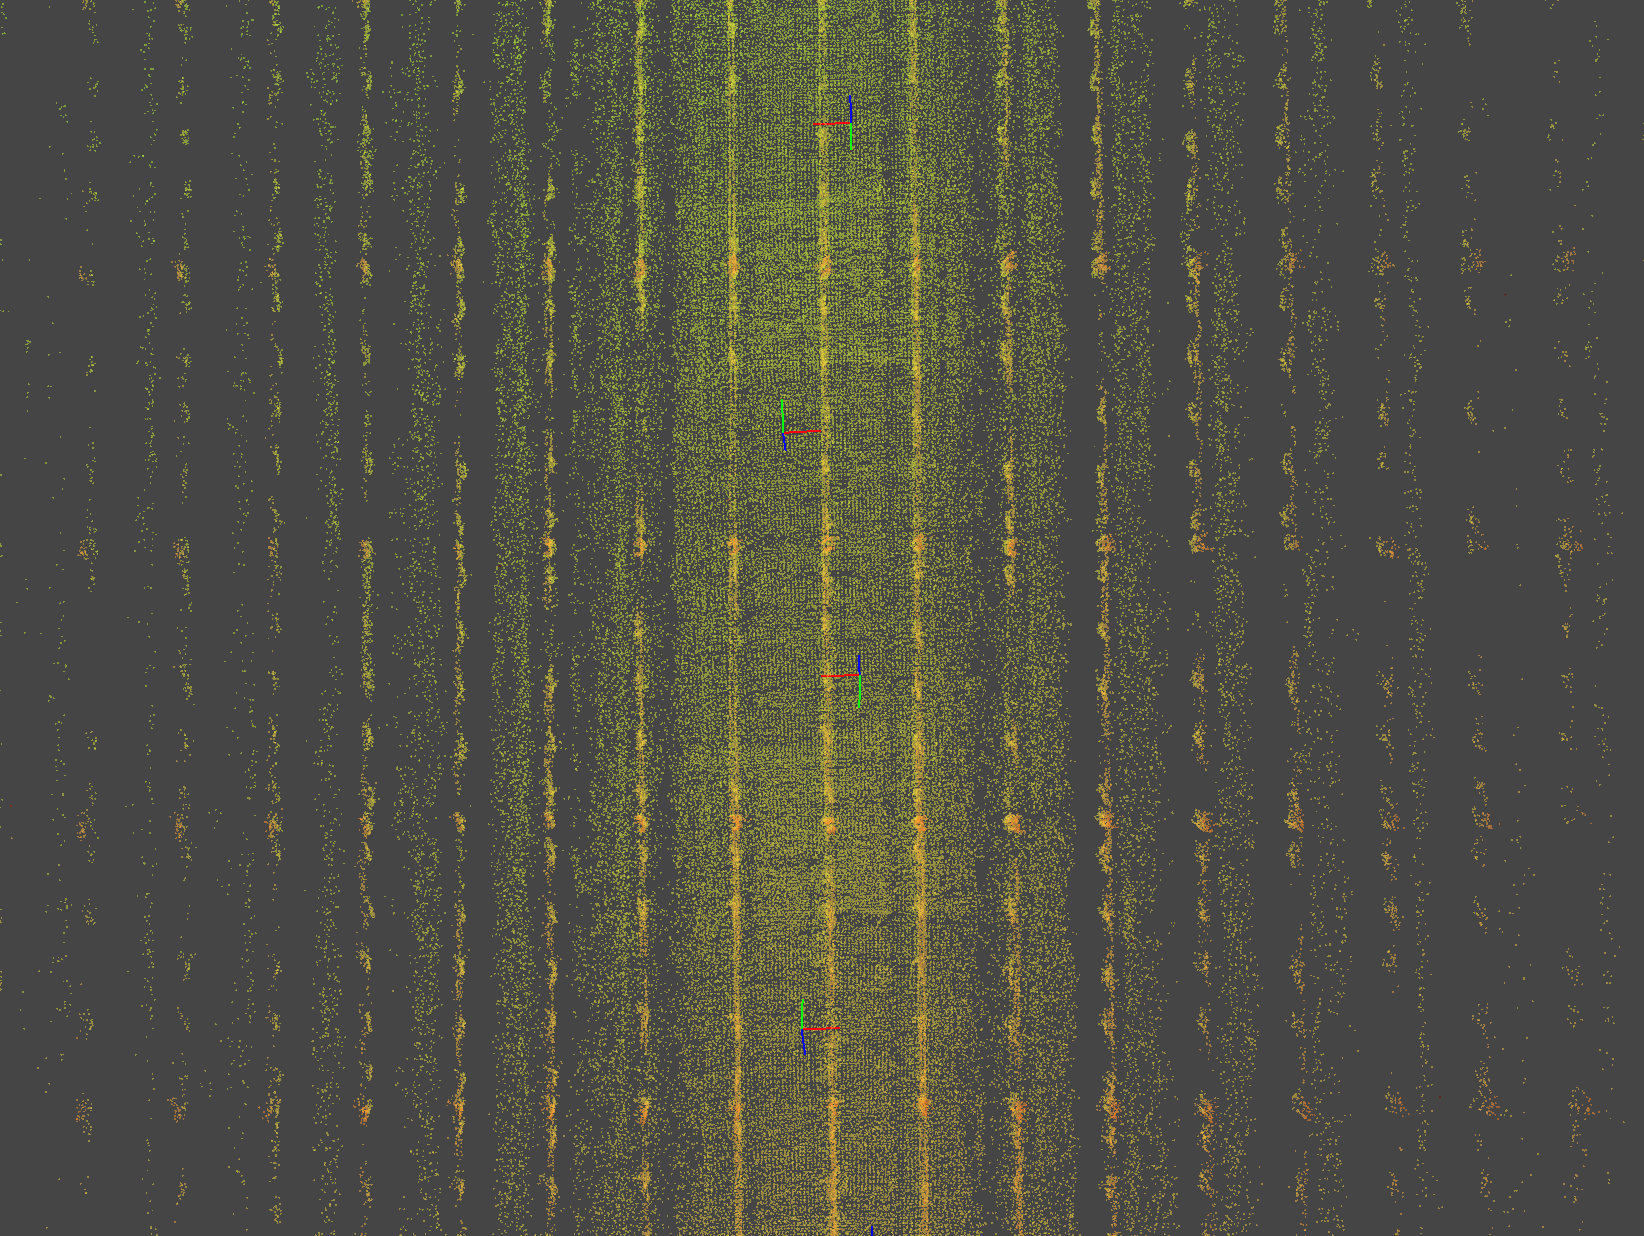
\includegraphics[width=0.85\linewidth]{3-SLAM/3-discussion/figures/zoomed_in_rows_SLAM_map.png}
    \caption{Bird's-eye view of the LiDAR point cloud map captured in the UCVision vineyard. The repetitive, corridor-like geometry of the rows is clearly visible: each row presents an identical wall of vegetation returns, with no distinctive geometric feature to discriminate one row from another. This perceptual aliasing is the root cause of the row-skipping failure described above.}
    \label{fig:zoomedRowsSLAMMap}
\end{figure}

\subsection{Refined GLIM Performance}
\label{subsec:slam-discussion-refined}

The transition from the baseline GLIM algorithm to the refined (parameterised) version demonstrates a marked improvement in localisation stability and drift suppression. While the baseline algorithm frequently succumbed to the failure modes described in previous sections, the refined version exhibits a more controlled error accumulation. Full performance metrics for all datasets are reported in \cref{tab:refined_performance}.

The most prominent improvement is observed in the \textit{error percent per metre} metric. In the baseline configuration, Dataset 2 exhibited a peak error of 7.3610\%, whereas the refined version reduced this to 3.6150\%, a reduction of approximately 50\%. In more favourable conditions, such as Dataset 4, the error dropped from 4.1910\% in the baseline to 0.6680\% in the refined version. This indicates that parameter optimisation effectively mitigates the ``point of no return'' by maintaining better geometric alignment over longer durations.

The \textit{RPE 1\,m translation standard deviation} serves as a proxy for the ``smoothness'' or ``jitter'' of the trajectory. While the baseline GLIM suffered from jagged trajectories around points of failure, peaking at a standard deviation of 0.9384 in Dataset 3, the refined GLIM consistently lowered this jitter across all datasets. For example, in Dataset 3, the refined version achieved an RPE standard deviation of 0.8239. The overall reduction suggests that the optimised parameters facilitate more reliable and consistent scan-matching, reducing the frequency of the ``jumps'' caused by false-positive matches in repetitive environments.

The \textit{error per metre (m)} metric further reinforces these findings. The refined GLIM consistently achieved sub-centimetre drift per metre in datasets where the baseline was drifting several centimetres (e.g., Dataset 0 dropping from 0.0340~m to 0.0087~m). This suggests that the refinement process successfully tuned the SLAM parameters to better suit the specific LiDAR characteristics and environment structure, delaying the onset of the catastrophic failures observed in the baseline.

\begin{table}[htbp]
\centering
\caption{Comparative Performance: Baseline vs. Refined GLIM}
\label{tab:comparison_summary}
\begin{tabularx}{\textwidth}{lXXXXX}
\toprule
\textbf{Metric} & \textbf{Dataset 0} & \textbf{Dataset 1} & \textbf{Dataset 2} & \textbf{Dataset 3} & \textbf{Dataset 4} \\ \midrule
\textbf{Error \% Reduction} & 73.9\% & 51.4\% & 50.8\% & 84.6\% & 84.0\% \\
\textbf{RPE Std Improvement} & 12.2\% & 5.8\% & 28.8\% & 12.2\% & 19.9\% \\ \bottomrule
\end{tabularx}
\end{table}

\subsection{GLIM-GNSS: GNSS-Augmented Localisation}

By introducing a source of absolute positional observability absent from both the baseline and refined GLIM configurations, GLIM-GNSS eliminates the unbounded drift inherent in scan-matching-only odometry. The resulting improvement is approximately two orders of magnitude in localisation accuracy relative to the untuned GLIM baseline (0.015–0.050\% vs.\ 1.3–7.4\%), and approximately one order of magnitude relative to the refined GLIM (0.015–0.050\% vs.\ 0.6–3.6\%). It is important to note that this comparison is not purely algorithmic: GLIM-GNSS leverages sparse GNSS factor injection as an additional sensor input, providing absolute positional observability that is unavailable to both the baseline and refined configurations. The improvement therefore reflects the combined effect of GNSS integration and parameter optimisation, rather than algorithmic changes alone. The GLIM-GNSS system's error percentage per metre ranges from $0.0153\%$ (Dataset 4) to $0.0501\%$ (Dataset 2) (see \cref{tab:proposed_performance}), compared to the refined GLIM's range of $0.6081\%$ to $3.6150\%$. This reduction is consistent across all datasets, with no observable catastrophic failure modes analogous to those seen in earlier iterations.

\subsubsection{GNSS Integration}

Whereas baseline GLIM operates exclusively on scan-matching odometry, GLIM-GNSS augments the submaps and keyframes' local relative information with periodic absolute position measurements from the GNSS receiver. This integration serves two distinct functions: (1) it grounds the map frame in a fixed real-world coordinate system, ensuring trajectory estimates are metrically consistent with the farm's local ENU reference rather than an arbitrary per-run origin; and (2) because GNSS measurements enter as factors in a graph optimiser rather than as Kalman filter updates, their effect propagates non-causally, correcting prior states within the optimisation window rather than only conditioning future estimates.

The effectiveness of this approach is evident in comparing error accumulation results. In the refined GLIM, even with parameter optimisation, the error percent per metre remains linear or superlinear across the traversal. By contrast, GLIM-GNSS maintains sub-centimetre per-metre errors throughout, suggesting that the global constraints are sufficiently frequent and accurate to prevent drift from establishing itself in the first place.

This result is further reinforced by the GNSS factor utilisation statistics (\cref{tab:gnss_stats}): across all datasets, between 0.65--0.78\% of all available GNSS data points were injected into the factor graph following outlier rejection. This sparsity is itself a key achievement of this work. A primary motivation for the GLIM-GNSS architecture was to reduce operational dependence on RTK-GNSS, which is subject to signal degradation from canopy occlusion, multipath interference, and adverse weather, as well as high infrastructure costs in agricultural deployments. The results demonstrate that the vast majority of localisation accuracy is recovered through the LiDAR-inertial odometry backbone, with GNSS contributing only infrequent global anchors to prevent long-term drift accumulation. Achieving one to two orders of magnitude improvement over the baseline and refined GLIM configurations, respectively, at sub-percent GNSS utilisation confirms that dense or continuous RTK coverage is not a prerequisite for precise trajectory estimation in the GLIM-GNSS architecture.

\subsubsection{Dataset-Specific Performance Variability}

Despite the strong performance of GLIM-GNSS across all datasets, performance does vary across datasets in a pattern that suggests environmental factors influencing localisation quality. Dataset 2 exhibits the highest error metrics (0.0501\% error per metre, RMSE $y$ of 0.2003~m, ATE of 0.1741~m), whereas Dataset 3 achieves the lowest error (0.0134\% error per metre) and Dataset 1 the second lowest (0.0154\%). 

The degradation in Dataset 2 is likely due to environmental conditions rather than algorithmic limitations. Dataset 2 also recorded the fewest raw GNSS measurements prior to outlier rejection (7,236 points, compared to 9,241--13,461 across the remaining datasets; see \cref{tab:gnss_stats}), providing independent evidence of reduced signal availability rather than merely an elevated rejection rate. The low factor utilisation (0.65\% of available GNSS data points injected into the factor graph, the lowest across all datasets) is therefore consistent with canopy occlusion or multipath interference reducing the absolute number of receivable signals along that route. The geometric consistency-based outlier rejection, whilst effective at filtering genuinely erroneous points, cannot recover lost signal availability. Even under these challenging conditions, the localisation error remained controlled at $0.0501\%$, indicating robustness to transient GNSS degradation.

\subsubsection{Relative Pose Error}

The Relative Pose Error (RPE) metrics, which assess the consistency of local pose increments, provide insight into frame-to-frame localisation smoothness. GLIM-GNSS achieves RPE 1~m translation standard deviations ranging from $0.0205$ to $0.0479$~m across all datasets, compared to the refined GLIM's $0.2449$ to $0.8239$~m. This roughly tenfold to thirty-fivefold reduction in local pose jitter indicates that the global constraints are not merely correcting large-scale drift, but are improving the consistency of short-horizon relative measurements.

This improvement likely arises from the factor graph's ability to reason about odometric uncertainty jointly with global constraints. When the optimiser encounters a region where local odometry is inconsistent with global GNSS observations, it propagates the correction smoothly across the pose graph rather than applying isolated jump corrections. This smoothness is essential for downstream applications such as robotic arm control, where abrupt discontinuities in perceived position could cause trajectory tracking errors.

\subsubsection{GASP Metric Behaviour and Optimisation Dynamics}

A counterintuitive finding is a marginal upward trend in the GASP (Global Alignment and Smoothness Profile) metric for the single best-performing run across the four parameter optimisation stages (\cref{fig:comparison_progression}). Unlike the baseline GLIM error percentage, which exhibits clear convergence and monotonic improvement (\cref{fig:baseline_progression,fig:baseline_error_dist}), the GLIM-GNSS system's best-run GASP metric increases (degrades) marginally from stage one to stage four (\cref{fig:proposed_progression}). This trend could be due to the stochastic nature of the Latin Hypercube parameter search rather than to any systematic degradation. The differences between near-optimal configurations are negligible, and stage one may have already identified a configuration that performs near-optimally. Subsequent stages sample nearby regions of the parameter space and, by chance, return configurations that score marginally worse on GASP. The magnitude of the variation is small enough that it falls within the expected noise of the pseudo-random search process.

Despite this marginal decline in peak performance, the overall distribution of GASP metric values improves significantly across the four stages, as shown in \cref{fig:comparison_dist}. As shown in \cref{fig:proposed_error_dist}, the error distributions shift progressively leftward over successive stages, indicating an improvement in typical performance. Concurrently, the distributions become taller and narrower — that is, the standard deviation decreases — reflecting an increase in the reliability and consistency of results. In contrast, the stage zero distribution is comparatively flat and wide, indicating that results at that stage were highly variable and unpredictable. This evolution demonstrates that the optimisation process is not identifying a single lucky configuration, but is systematically converging the parameter space towards a regime in which good performance is reproducible. The trade-off between peak and median performance is therefore a natural consequence of this convergence: as the search focuses on consistently high-performing regions, extreme but unreliable high-performing outliers are replaced by a tighter cluster of reliably good solutions.

\subsection{Comparative Analysis and Mechanisms of Improvement}

The experimental results, summarised in \cref{tab:comparison_table_key_metrics} and visualised across all metrics and datasets in \cref{fig:comparison_spider}, reveal a clear hierarchy of performance and illustrate the mechanisms driving improvements at each stage.

\subsubsection{Parametrisation vs. Sensor Fusion}

The transition from baseline to refined GLIM demonstrates that parameter tuning can reduce error magnitude significantly (50--85\% reduction in error percentage per metre; see \cref{fig:spider_ep} and \cref{fig:spider_epm}). However, parameter optimisation alone does not eliminate the fundamental instability of scan-matching-only odometry in repetitive vineyard environments. The refined GLIM still exhibits occasional trajectory inconsistencies and elevated RPE and ATE metrics relative to GLIM-GNSS (see \cref{fig:spider_RPE_std} and \cref{fig:spider_ATE}).

By contrast, the transition from refined GLIM to the GNSS-augmented GLIM-GNSS represents a qualitative shift in localisation architecture. Rather than optimising the tuning parameters of a single sensor modality, GLIM-GNSS introduces a fundamentally independent source of global position information. This architectural change achieves improvements that parametrisation alone cannot reach. The reduction in error percentage per metre from refined GLIM to GLIM-GNSS ($\sim$97--99\%) is larger and more consistent than the corresponding improvement from baseline to refined GLIM ($\sim$51--85\%), and GLIM-GNSS exhibits no dataset in which performance degrades significantly.

\subsubsection{Role of Outlier Rejection}

The geometric consistency-based outlier rejection procedure is critical in ensuring that only reliable GNSS measurements are incorporated into the factor graph. This aggressive filtering makes the sparse utilisation viable; by ensuring that every incorporated constraint is geometrically consistent, the procedure prevents a single erroneous global measurement from corrupting the factor graph. The architecture therefore achieves the desired property of sparse GNSS integration, using the global sensor as an infrequent but reliable anchor for the scan-matching-based odometry. This deterministic filtering approach, based on rigid-body distance preservation, is well-suited to the repetitive vineyard environment, where probabilistic alternatives such as RANSAC would require outlier distribution assumptions that may not hold in structured agricultural settings.

The robustness of this design is confirmed by Dataset 2, where GNSS factor utilisation falls to its lowest observed value of 0.65\%, yet localisation error remains controlled at $0.0501\%$ per metre. This indicates that each geometrically verified constraint carries sufficient positional information to anchor the trajectory even when GNSS availability is degraded.

\subsection{Generalisation to the Evaluation Dataset}
\label{subsec:slam-generalisation}

Beyond performance on the parameterisation datasets, the three configurations were evaluated on a held-out Evaluation Dataset to assess whether the observed improvements are specific to the training data distribution or generalise to previously unseen routes. The results are reported in \cref{subsec:slam-eval-results}; the analysis here focuses on what they reveal about generalisation behaviour.

\subsubsection{Overall Performance Hierarchy}

The three-tier performance ranking observed across the parameterisation datasets — baseline GLIM performing worst, refined GLIM intermediate, and GLIM-GNSS achieving the lowest errors — is broadly preserved on the Evaluation Dataset (see \cref{tab:eval_comparison_key_metrics}). The ordering holds for error percentage per metre and error per metre. For RPE 1\,m translation standard deviation, however, the refined GLIM's mean (0.4019) exceeds that of the baseline (0.1093) due to the influence of at least one catastrophic failure run, which inflates the aggregate statistic beyond the baseline's more uniformly distributed error. GLIM-GNSS achieves the lowest value on all three metrics. This overall consistency indicates that neither the parameterisation process nor the GNSS integration architecture produces results that are specific to the routes on which they were developed.

\subsubsection{Baseline GLIM}

The baseline GLIM mean error percentage per metre on the Evaluation Dataset falls within the range observed on the parameterisation datasets (1.253\%--7.361\%) and is comparable to the middle-tier parameterisation datasets (see \cref{tab:eval_baseline_performance}), indicating no systematic degradation on unseen data. This is expected: the baseline configuration involves no parameter tuning, so there is no mechanism by which its behaviour could be route-specific. The modest run-to-run variability is consistent with the stochastic nature of the scan-matching front-end.

\subsubsection{Refined GLIM}

The mean error percentage per metre for the refined GLIM on the Evaluation Dataset is consistent with the parameterisation dataset range (0.608\%--3.615\%), indicating that the optimised parameters transfer well in terms of mean performance (see \cref{tab:eval_refined_performance}).

Nonetheless, the results also reveal a significant instability that is not captured by the mean error percentage alone. As reported in \cref{tab:eval_refined_performance}, the maximum 3D positional error exhibits a mean--median discrepancy of approximately threefold (39.59\,m vs.\ 13.09\,m), with a maximum observed value of 148.61\,m. This pattern indicates that at least one of the five runs experienced a catastrophic failure of the type described in \cref{subsec:slam-discussion-refined} — a sudden and irrecoverable collapse of scan-matching alignment leading to unbounded planar drift. The same failure signature is visible in the RPE metrics, where mean values are an order of magnitude larger than the corresponding medians, confirming that the elevated aggregates are driven by a tail event rather than uniformly elevated error.

This apparent bimodal behaviour — the majority of runs performing well, with an occasional catastrophic failure — is arguably a more concerning failure mode in practice than a uniformly elevated error, because it is unpredictable at deployment time. The small sample size ($n = 5$) limits formal distributional characterisation, but the magnitude of the outlier (max positional error exceeding the median by a factor of eleven) is sufficient to establish that the failure mode persists on unseen routes. An operator relying on the refined GLIM cannot distinguish an impending failure run from a well-behaved one prior to the failure event. The parameter optimisation delays the onset of the instability described in the parameterisation dataset analysis but does not eliminate the underlying scan-matching vulnerability in semi-structured vineyard environments. Whether the catastrophic run can be attributed to specific environmental factors along the Evaluation Dataset route — such as a stretch of low-geometric-excitation terrain or a section with reduced inter-row distinctiveness — cannot be determined from aggregate statistics alone and would require per-run trajectory inspection.

\subsubsection{GLIM-GNSS}

The GLIM-GNSS system's Evaluation Dataset performance falls within and is consistent with the parameterisation dataset range of 0.0153\%--0.0501\% for error percentage per metre (see \cref{tab:eval_proposed_performance}). The standard deviation across five runs is less than 2.5\% of the mean value, indicating near-deterministic behaviour. This contrasts sharply with the refined GLIM, where the corresponding metric standard deviation accounts for approximately 17.5\% of the mean. The GASP metric likewise falls within the parameterisation dataset range (0.0274--0.0679), confirming consistent behaviour on both local and global accuracy dimensions.

This near-deterministic behaviour confirms a practically important property of the GLIM-GNSS architecture: the GNSS global constraint effectively suppresses the non-deterministic component of the underlying odometry pipeline. An operator deploying the system can therefore expect consistent performance across repeated runs rather than a distribution of outcomes that may occasionally include a failure event.

The error percentage per metre on the Evaluation Dataset is directly comparable to the parameterisation results, with no evidence of performance degradation on held-out data. Since the Evaluation Dataset was collected at the same farm, these results demonstrate route-level rather than cross-environment generalisation.

\subsection{Limitations and Implications for Vineyard Robotics}

The GLIM-GNSS system's consistent sub-centimetre drift rate (error per metre of traversal) has direct implications for robotic pruning feasibility. This per-metre drift must be distinguished from absolute trajectory error: while the per-metre error remains below 1~mm across all datasets, the cumulative position error over a full traversal reaches approximately 0.7--1.0~m. Pruning tasks require localisation accuracy sufficient to position the robotic arm within reach of target vine structures. With typical vine stems ranging from 5--15~mm in diameter, this absolute error bound can be accommodated through local perception-based arm guidance or online trajectory adjustment based on close-range stereo or depth sensing.

A fundamental limitation of the evaluation presented in this chapter is that all reported metrics are restricted to translational quantities: ATE measures absolute positional accuracy relative to ground truth, RPE and error per metre quantify relative translational drift, and the Global Alignment and Smoothness Profile (GASP) combines normalised drift rate and translational RPE standard deviation into a single relative performance index. The evaluation does not assess rotational pose accuracy (roll, pitch, and yaw). For high-level navigation and path planning, translational accuracy is the primary concern, and the reported results are sufficient to characterise coarse localisation quality. However, for fine-grained manipulation tasks such as autonomous pruning, the full six-degree-of-freedom pose of the robot relative to a vine structure is required. A position estimate that is globally accurate but accompanied by an unquantified orientation error may still be insufficient to guide a robotic arm to within the centimetre-level precision needed to interact with individual vine shoots.

A second methodological consideration is that the ground truth trajectory used for evaluation is itself derived from real-time RTK-GNSS fixes, while GLIM-GNSS also incorporates GNSS measurements as sparse factors. This apparent circularity does not invalidate the evaluation for two reasons: (1)~the ground truth uses the complete, continuous RTK fix stream at full receiver rate, whereas GLIM-GNSS injects fewer than 1\% of available GNSS fixes as discrete factor-graph constraints after geometric outlier rejection; the information content available to each is therefore fundamentally different; and (2)~the primary comparison is between GLIM-GNSS and the refined GLIM, which shares the same ground truth but receives no GNSS input, isolating the effect of sparse GNSS integration on localisation accuracy.

In summary, the experiments in this chapter establish a three-tier performance hierarchy: the baseline GLIM algorithm exhibits unbounded drift in repetitive vineyard environments, the refined GLIM partially suppresses this instability through parameter optimisation but remains susceptible to catastrophic failure, and GLIM-GNSS achieves consistent sub-centimetre per-metre drift rates by grounding the factor graph with sparse but geometrically verified global constraints. This hierarchy is preserved on a held-out evaluation route, where GLIM-GNSS exhibits near-deterministic behaviour in contrast to the stochastic failure distribution of the refined GLIM. The principal gap in this evaluation, specifically unquantified rotational accuracy, directly motivates the fine-grained alignment approach presented in the following chapter.

Chapter~4 addresses this limitation by evaluating precise alignment techniques that estimate the full six-degree-of-freedom robot pose relative to a pre-existing 3D model of the vine structure, operating with no additional GNSS input and using local dense perception to constrain pose estimation.
\clearpage

\section{Summary}
\label{sec:slam-summary}

This chapter presented the design and implementation of a LiDAR-centric SLAM pipeline for GNSS-degraded operation and evaluated three configurations: the baseline GLIM system, a refined parameterised variant, and GLIM-GNSS. The results across five parameterisation datasets showed that parameter refinement reduced drift and improved trajectory smoothness relative to the baseline, while GLIM-GNSS achieved the lowest errors across all reported metrics, noting that this improvement reflects both algorithmic changes and the introduction of sparse GNSS factors as an additional sensor input unavailable to the baseline configurations. Evaluation on a held-out Evaluation Dataset confirmed that the performance hierarchy generalises to unseen routes, with GLIM-GNSS additionally demonstrating near-deterministic run-to-run consistency. The discussion highlighted characteristic failure modes in structured vineyard environments, the distinction between mean accuracy and run-to-run robustness, and the trade-off between peak and median performance arising from the parameter optimisation process.

\chapter{Precise Alignment}
\label{chap:precise-alignment}

\section{Introduction}
\label{sec:precise-alignment-intro}

The previous chapter established a LiDAR-inertial SLAM pipeline capable of performing without continuous GNSS availability, providing robust trajectory estimation and semi-dense environmental mapping across vineyard rows. While this system delivers the localisation accuracy required for autonomous navigation between vines, it does not, by itself, provide the centimetre-scale spatial accuracy necessary for robotic pruning. When a manipulator arm must reach a specific cane at a specific cut-point, the acceptable localisation error is smaller than what global SLAM can guarantee. This chapter aims to address that gap through a second-stage localisation refinement step that aligns the robot's perception of its environment with a pre-built high-fidelity vine model.

Whereas the SLAM system presented in \cref{chap:SLAM} is designed to operate across the full annual growth cycle of the vine, the precise-alignment stage described here is explicitly scoped to the winter pruning season. Robotic pruning is inherently a winter task: grapevines are pruned during dormancy, when they have shed their foliage and only the bare woody cane and trunk structure remains. The point cloud registration pipeline presented in this chapter exploits that leafless condition, as bare-wood geometry provides clean, unoccluded structure for alignment. All experiments and pipeline design decisions therefore assume dormant-season vine structure; vines carrying a full canopy are outside the scope of this work.

\subsection{System Context}
\label{subsec:system-context}

Central to the pruning localisation workflow described in this thesis is a 3D Gaussian Splatting (3DGS) model of each vine, constructed offline from imagery collected during a prior scanning pass. The reconstruction pipeline applies Structure from Motion (SfM) photogrammetry to these images, recovering a dense 3D point cloud and camera trajectory via bundle adjustment. The resulting point cloud forms the geometric backbone of the 3DGS model and is registered within a global Local East-North-Up (ENU) reference frame. Because SfM jointly optimises camera poses and 3D structure through reprojection minimisation, the reconstructed geometry is internally consistent and, once georeferenced, constitutes a reliable proxy for the true physical vine geometry. All downstream tasks — cut-point detection, path planning for the robotic arm, and collision avoidance — are computed against this 3DGS model in simulation. For these simulated operations to correspond faithfully to the real world, the robot's pose relative to the simulated vine (i.e.\ the 3DGS reconstruction) must match its true pose relative to the physical vine.

When the robot arrives at a target vine during an autonomous pruning mission, its pose is known only to the accuracy of the SLAM system described in \cref{chap:SLAM}. This accuracy is sufficient for navigation but insufficient for manipulation. The precise-alignment stage presented here corrects the residual misalignment by registering a real-time point cloud of the physical vine, acquired at the site, against the SfM point cloud extracted from the 3DGS model. The resulting rigid-body transformation is used to update the robot's estimated pose, thereby aligning the simulated and physical scenes before any pruning motion is executed. The overall system context is illustrated in \cref{fig:pa-system-context}.

\begin{figure}[htbp]
  \centering
  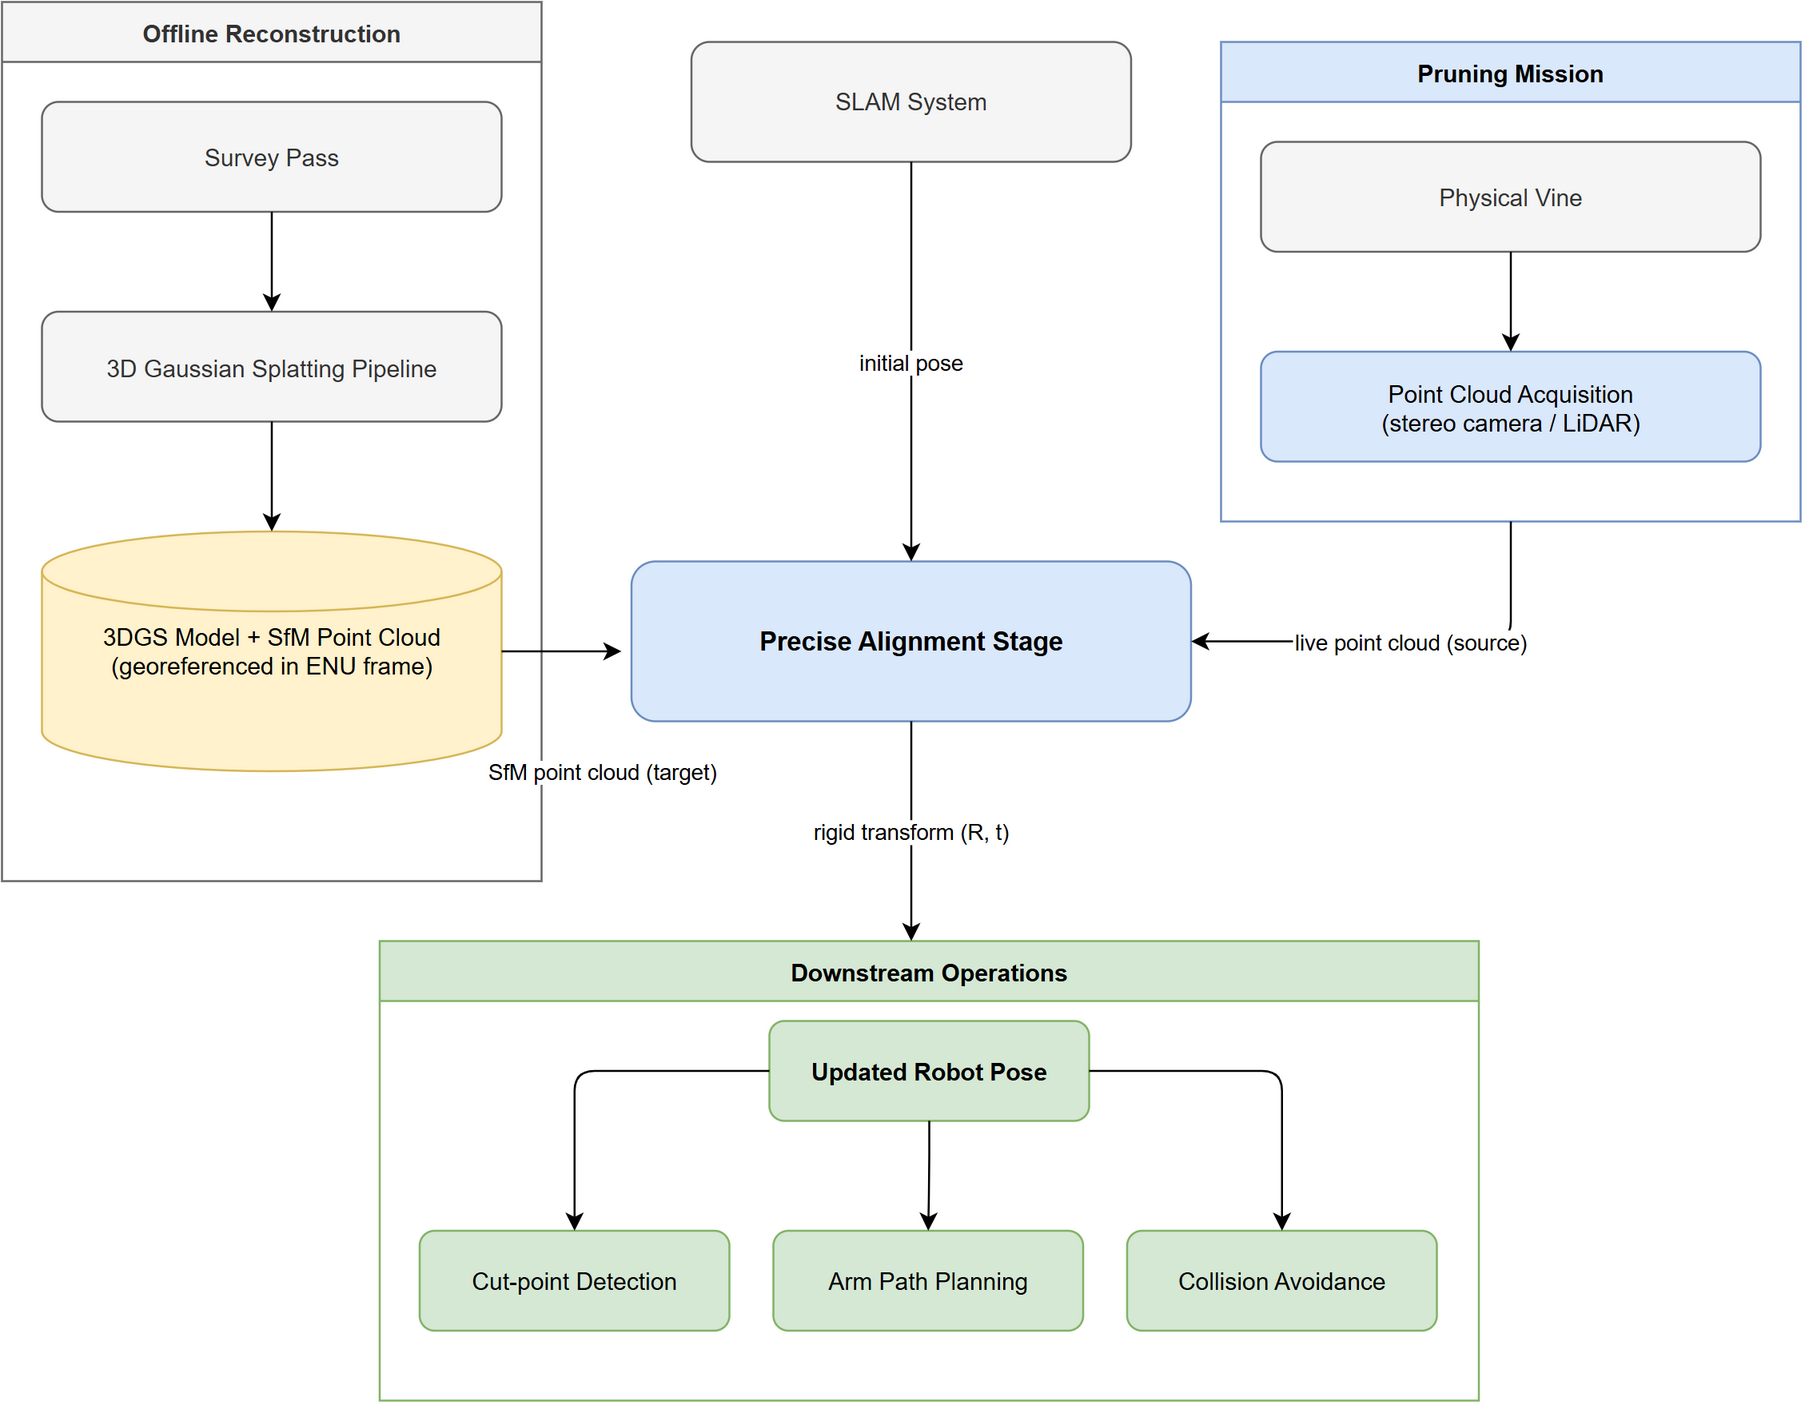
\includegraphics[width=\linewidth]{4-precise-alignment/4-intro/figures/pa-system-context}
  \caption{System context for the precise-alignment stage. Offline 3DGS
           reconstruction and a SLAM-derived initial pose are combined with a
           live sensor point cloud to produce a refined pose for downstream
           manipulation.}
  \label{fig:pa-system-context}
\end{figure}

\subsection{Approach Overview}
\label{subsec:approach-overview}

The precise-alignment pipeline proceeds through the following stages, as illustrated schematically in \cref{fig:pa-approach-overview}:

\begin{enumerate}
    \item The robot halts in front of the target vine and acquires a dense point cloud of the vine structure. Two sensing modalities are evaluated in this chapter: depth point clouds generated from a stereo camera, and dense maps built from a hybrid solid-state LiDAR sensor (Livox Mid-360).
    \item The acquired point cloud is passed through a modality-specific preprocessing pipeline that isolates the vine's structural geometry by removing noise and non-structural clutter, and downsamples the pointcloud to a resolution suitable for registration.
    \item The preprocessed source cloud is registered against the target cloud derived from the SfM reconstruction of the 3DGS model using the Generalised Iterative Closest Point (GICP) algorithm \cite{segalGeneralizedICP2009}.
    \item The recovered transformation is applied to update the robot's internal localisation, correcting its estimated pose relative to the vine. This updated pose is consumed by the arm path planner, ensuring that simulated cut-points correspond to their physical counterparts.
\end{enumerate}

\begin{figure}[htbp]
  \centering
  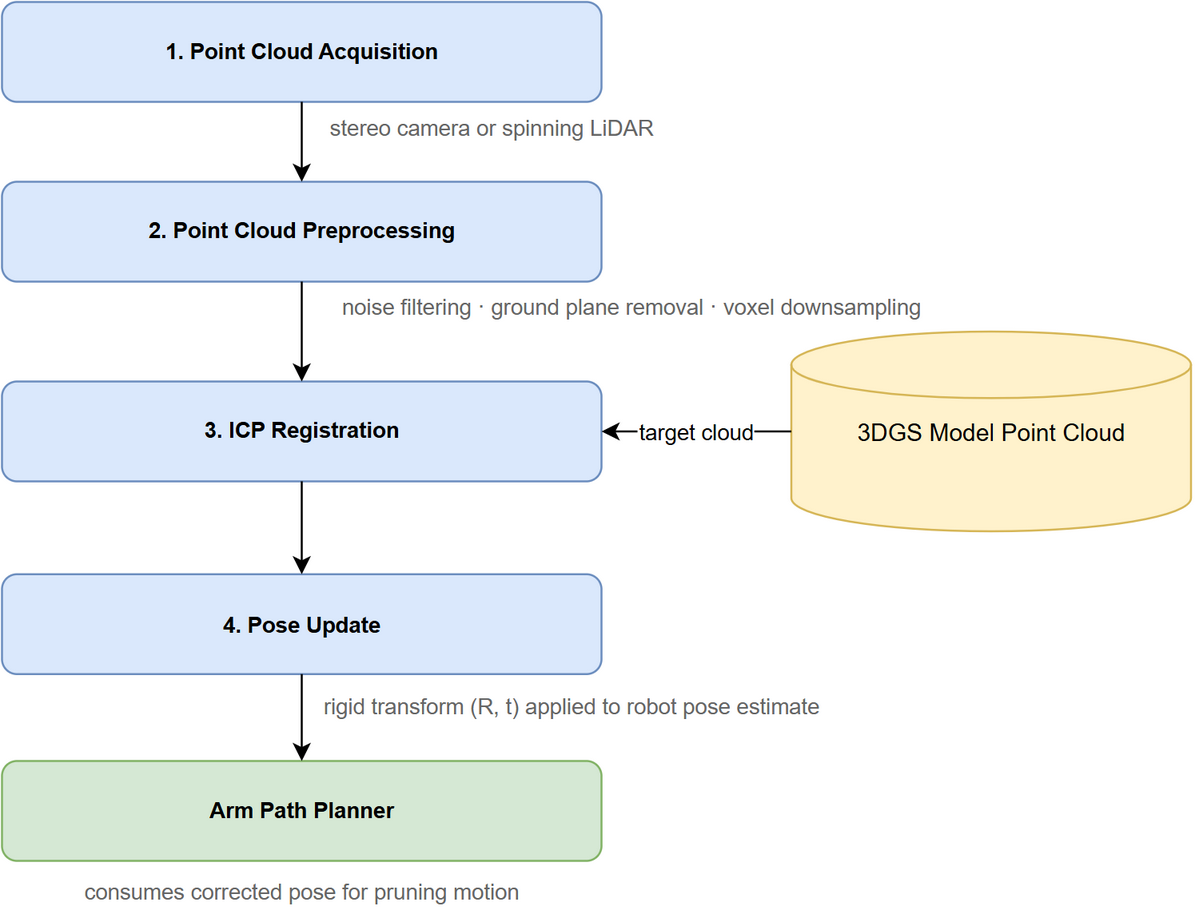
\includegraphics[width=0.65\linewidth]{4-precise-alignment/4-intro/figures/pa-approach-overview}
  \caption{Overview of the four-stage precise-alignment pipeline}
  \label{fig:pa-approach-overview}
\end{figure}

Each stage of this pipeline draws on a distinct body of prior work. This chapter is structured as follows. \Cref{sec:precise-alignment-related-work} reviews prior work on point cloud registration for agricultural and robotic applications, with particular attention to ICP variants and vine-specific sensing modalities. \Cref{sec:precise-alignment-methodology} details the full data processing and registration pipeline, including sensor configuration, preprocessing steps, and ICP parameterisation. \Cref{sec:precise-alignment-results} presents quantitative and qualitative results for both sensing modalities across a set of vineyard test cases. \Cref{sec:precise-alignment-discussion} discusses the relative merits and failure modes of each approach, and \cref{sec:precise-alignment-summary} summarises the key findings.

\section{Related Work}
\label{sec:precise-alignment-related-work}

The precise global localisation of a robotic platform within a vineyard environment can be broken down into three technical problems. First, the robot must generate detailed, metrically scaled three-dimensional representations of the vine and/or environment from its onboard sensors. Second, a global structural reference map must already exist against which those local observations can be compared. Third, reliable algorithms must compute the rigid transformation that aligns the local capture to the global frame, recovering the robot's pose with centimetric accuracy. This section reviews each problem as follows: proximal (close-range, ground-level) three-dimensional sensing via stereo, RGB-D, and LiDAR modalities; the construction of dense reference maps from LiDAR and photogrammetric pipelines; and the class of point cloud registration algorithms built upon the Iterative Closest Point (ICP) framework.

\subsection{Stereo Depth Imaging}
\label{subsec:stereo-depth}

Stereo and RGB-D imaging systems are widely used to generate three-dimensional models of individual plants. Depth is recovered from the disparity $d$ between corresponding pixels in a rectified stereo pair, related to metric depth $Z$ by the standard pinhole model equation:
%
\begin{equation}
    Z = \frac{f \cdot B}{d},
\end{equation}
%
where $f$ is the focal length and $B$ is the baseline between the two image sensors.

Klodt et al.~\cite{klodtFieldPhenotypingGrapevine2015} established that passive stereo cameras are sufficient for quantitative vine characterisation under realistic outdoor conditions, generating dense depth maps from paired RGB images without requiring a controlled background or calibration rig. Parr et al.~\cite{parrAnalysisDepthCameras2022} subsequently benchmarked five depth sensor modalities on grape clusters under both laboratory and open-field conditions, comparing structured light, active-infrared (IR) stereo, time-of-flight, and LiDAR-based sensors. Their results showed that the RealSense D415 active IR stereo sensor achieved approximately 2\,mm error in controlled indoor conditions and remained functional in full sunlight, whereas time-of-flight and structured-light sensors exhibited larger measurement bias. These comparative findings provide an empirical basis for depth sensor selection in precise mapping vineyard tasks. Active RGB-D sensors (e.g., Azure Kinect) offer artificial texture projection for feature-poor scenes but suffer systematic depth failures under direct sunlight~\cite{tolgyessyEvaluationAzureKinect2021}, making passive stereo the more practical modality for outdoor vineyard deployment.

More recently, foundation model approaches have been applied to stereo depth estimation with the goal of achieving reliable zero-shot generalisation across varied imaging conditions. FoundationStereo~\cite{wenFoundationStereoZeroShot2025}
addresses the sim-to-real transfer problem by training on a curated dataset of one million photorealistic synthetic stereo pairs and employing a Side-Tuning Adapter (STA) to leverage monocular depth priors from DepthAnything V2; cost volumes are subsequently filtered via an Attentive Hybrid Cost Filtering (AHCF) module combining Axial-Planar Convolutions with a Disparity Transformer for long-range disparity reasoning. The model demonstrates strong zero-shot generalisation across the Middlebury and ETH3D benchmarks, with a separately fine-tuned variant achieving state-of-the-art on ETH3D, and performs well on in-the-wild data, as illustrated in \cref{fig:zeroShotFS}. In the present work, FoundationStereo is applied to imagery from a ZED Mini stereo camera to produce the depth maps from which the source point cloud is derived prior to registration.

\begin{figure}[htbp]
    \centering
    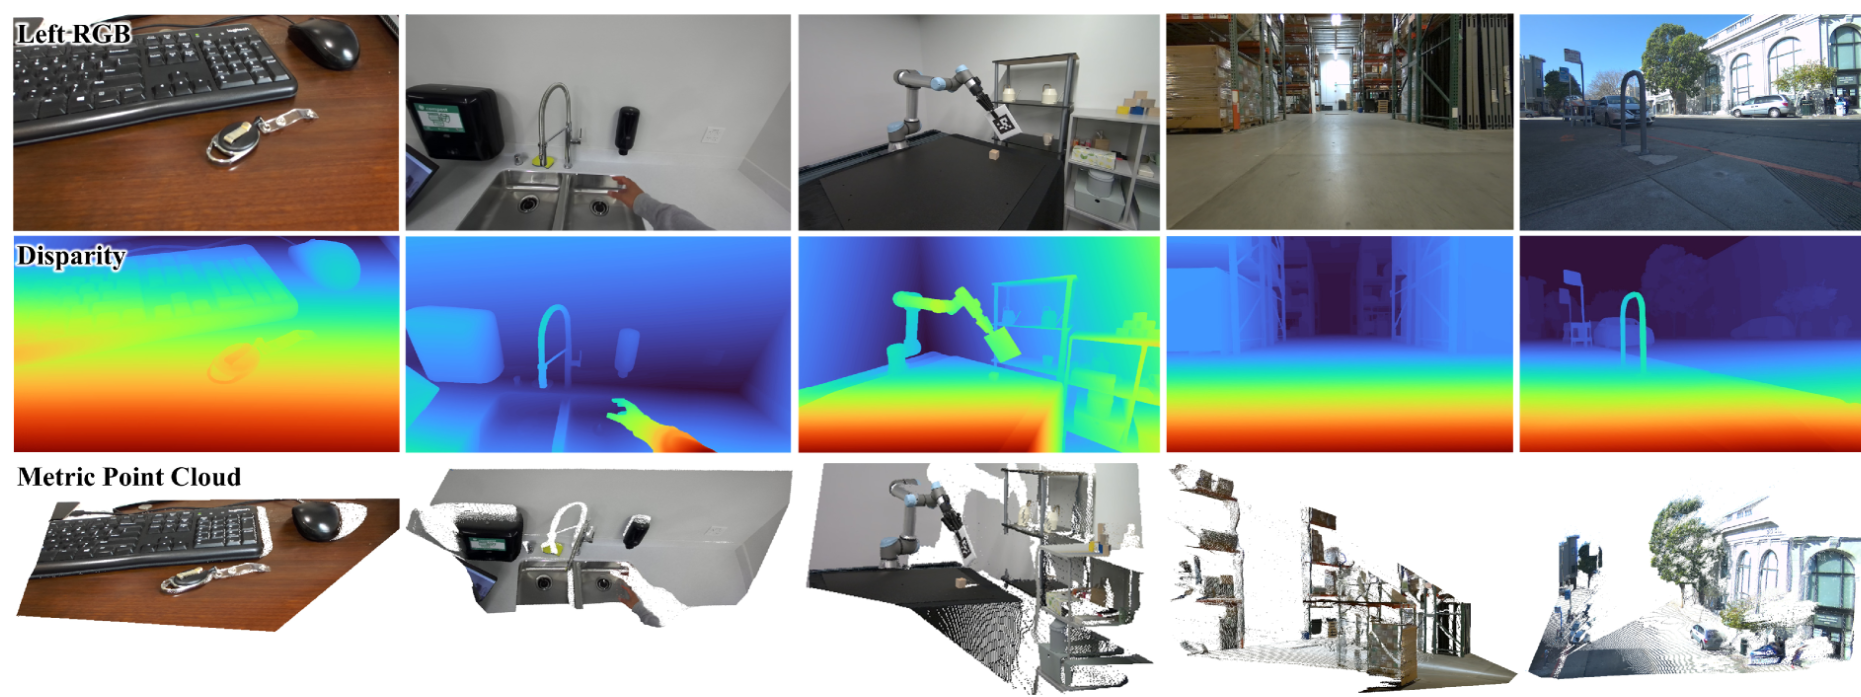
\includegraphics[width=0.9\linewidth]{4-precise-alignment/4-related-work/figures/zeroShotFSImages.png}
    \caption{Zero-shot stereo depth predictions from FoundationStereo across diverse in-the-wild scenes, including indoor and outdoor environments, textureless and reflective surfaces, and challenging illumination conditions. No per-domain fine-tuning is performed \protect\cite{wenFoundationStereoZeroShot2025}.}
    \label{fig:zeroShotFS}
\end{figure}

\subsection{Dense LiDAR Mapping}
\label{subsec:dense-lidar-mapping}

The preceding chapter employed LiDAR for real-time odometry and mapping; this subsection considers its complementary role in constructing the dense, 
centimetre-resolution reference models against which the robot subsequently localises. Unlike stereo imaging, LiDAR measures physical geometry rather than visual appearance and is therefore substantially more robust to scene texture variation; however, highly reflective, specular, or strongly light-absorbing surfaces can still produce erroneous returns, signal loss, or elevated noise in the resulting point cloud. LiDAR performs consistently during the dormant season when vine architecture is reduced to bare wood, which is precisely when precision pruning operations are carried out.

At the proximal sensing scale relevant to this thesis, Moreno et al.~\cite{morenoOnGroundVineyardReconstruction2020} demonstrated high-density 3D reconstruction of dormant vine rows using a downward-facing 2D time-of-flight LiDAR mounted on an electric platform georeferenced via RTK-GNSS. Applying $\alpha$-shape fitting to extract branch volumes, they reported a linear correlation with actual dry biomass of $R^2 = 0.85$, confirming that ground-level LiDAR produces geometrically faithful vine models at centimetre resolution. The sensor-to-canopy distances employed (0.5--1.5\,m) are comparable to the operating range evaluated in \cref{sec:precise-alignment-results}. Teng et al.~\cite{tengAccuracyEvaluationBranch2023} compared backpack-mounted 3D LiDAR SLAM against UAV-SfM for modelling dormant peach trees during winter pruning, finding that the ground-level LiDAR approach achieved higher geometric accuracy ($R^2 = 0.93$ against pruned branch fresh weight) with shorter acquisition time than the aerial photogrammetric alternative. Their results confirm that mobile LiDAR SLAM produces reference-quality models of bare-branch fruit tree structure at close range, and that branches with diameters exceeding 3\,cm are reliably resolved in the resulting point clouds.

Petrović et al.~\cite{petrovicVineCanopyReconstruction2022} directly compared terrestrial LiDAR and UAV photogrammetric reconstruction on defoliated vines, finding that both modalities achieve regression against ground-truth geometry of $R \approx 0.9$. This indicates that dense LiDAR-generated point clouds are a viable alternative to SfM for constructing global reference maps. The maps produced in that study span a survey area of 7\,m~$\times$~28\,m. Comparatively, the SfM-derived 3DGS reference map used in this thesis covers a single vineyard bay (three to four vines within the global ENU frame). 

No matter whether the real-time pointcloud model is created by a stereo camera or a LiDAR, the final alignment step requires a common algorithmic framework for registering the two point clouds.

\subsection{Point Cloud Registration}
\label{subsec:registration-methods}

The ICP algorithm and its foundational variants (point-to-plane and Generalised-ICP) were introduced in \cref{subsec:bg-point-cloud-registration}. This section reviews the broader landscape of registration methods that inform the design choices made in the precise-alignment pipeline.

Rusinkiewicz and Levoy~\cite{rusinkiewiczEfficientVariantsICP2001} provided an influential taxonomy of ICP design choices, classifying variants across point selection, correspondence matching, and minimisation strategy, and demonstrated that a well-chosen combination achieves alignment in a few tens of milliseconds. Huang et al.~\cite{huangComprehensiveSurveyPoint2021} surveyed both optimisation-based and deep learning registration methods, finding that optimisation-based approaches generalise well to novel scenes without training data, whereas learned methods degrade when the target scene differs from the training distribution. Their survey also identifies density difference and scale variation as the dominant challenges in cross-source registration, directly characterising the alignment problem in this thesis, where a dense stereo-derived point cloud must be registered against a photogrammetric reference model with fundamentally different density and noise characteristics.

Several extensions of ICP improve robustness in the geometrically repetitive, texturally ambiguous structure of vineyard rows. Beyond the Generalised-ICP formulation introduced in \cref{subsec:bg-point-cloud-registration}, which models local surface patches as Gaussian distributions and reduces sensitivity to incorrect correspondences, further variants augment the correspondence metric with additional geometric or photometric information. He et al.~\cite{heIterativeClosestPoints2017} proposed GF-ICP, a feature-augmented variant that incorporates point curvature, surface normals, and local density into the correspondence cost. This enriched error metric enables convergence from larger initial errors than pure geometric proximity allows. Choi et al.~\cite{choiIterativeKClosestPoint2020} extended ICP to coloured point clouds through a probabilistic K-closest matching formulation with a colour-supported objective, adding a photometric constraint that reduces correspondence ambiguity in regions with visually distinct surface texture, a useful property when aligning vine bark or cane surface reconstructions.

Semantic ICP, as developed by Chen et al.~\cite{chenSemanticICPIterativeClosest2025}, restricts correspondence matching to points sharing the same semantic class label. This prevents the structurally plausible but semantically incorrect matches. Vizzo et al.~\cite{vizzoKISSICPDefensePointtoPoint2023} demonstrated with KISS-ICP that a deliberately lean point-to-point formulation, augmented by adaptive correspondence thresholding and a robust kernel for outlier rejection, achieves competitive LiDAR odometry accuracy across diverse sensor platforms and environments without requiring per-deployment parameter tuning. Their finding that engineering simplicity can match or exceed more complex variants in practice has informed the design of several subsequent registration systems.

A fundamental limitation common to all ICP variants is sensitivity to the initial pose estimate: convergence to the global optimum of the ICP objective (\cref{eq:icp}) is not assured when the initial alignment error exceeds the geometric scale of distinctive scene features. For the more challenging case of global registration from an arbitrary initial pose, Mellado et al.~\cite{melladoSuper4PCSFastGlobal2014} introduced Super4PCS, which detects congruent four-point bases across two overlapping point clouds in linear time, enabling alignment in arbitrary initial orientations with as little as 25\% overlap. Yang et al.~\cite{yangGoICPGloballyOptimal2016} proposed Go-ICP, which employs a branch-and-bound search over the $SE(3)$ space of rigid transformations, guaranteeing globally optimal ICP solutions by systematically excluding sub-optimal rotation regions at the cost of increased computation.

The most recent direction adapts deep learning to replace hand-crafted descriptors with learned representations. Elbaz et al.~\cite{elbaz3DPointCloudRegistration2017} trained a deep auto-encoder to encode overlapping local regions of a point cloud into compact feature vectors; matched descriptor pairs initialise a subsequent ICP refinement, enabling robust alignment even under the large initial misalignment typical when registering a close-range scan against a large-scale prior map. Zhang et al.~\cite{zhangDeepLearningBased2020} provide a systematic review of deep learning-based registration methods, concluding that learned descriptors consistently outperform hand-crafted alternatives on standard benchmarks, in particular under noise and low-overlap conditions. Xu et al.~\cite{xuCross3DRegLargescaleRealworld2025} address the further challenge of cross-source registration, specifically aligning point clouds from heterogeneous sensor types, such as a spinning mechanical LiDAR and a semi-solid-state LiDAR, through a visual-geometric attention module that fuses image and geometric features to establish robust correspondences across point clouds with different density and pattern distributions. A global survey by Yin et al.~\cite{yinSurveyGlobalLiDAR2024} identifies the central open challenge in LiDAR-based global localisation as reliably retrieving the correct initial alignment hypothesis within a large-scale map, noting that the dominant operational approach (global place retrieval followed by local ICP refinement) remains fragile under seasonal appearance change, a challenge directly relevant to long-term autonomous deployment in vineyards.

\section{Precise-Alignment Pipeline}
\label{sec:precise-alignment-methodology}

The relocalisation pipeline described in this section refines the coarse initial pose estimate delivered by the SLAM system presented in \cref{chap:SLAM} through point cloud registration against a pre-built 3D Gaussian Splatting reference model. Two independent sensing modalities, stereo vision and accumulated LiDAR, are evaluated within a common architectural framework; both feed into a shared ICP registration backend, the output of which is used to correct the robot's estimated pose in the ROS~2 transform tree. The approach is outlined in \cref{subsec:approach-overview}; the following subsections present each component in detail.

% ---------------------------------------------------------------
\subsection{System Overview}
\label{subsec:pa-system-overview}
% ---------------------------------------------------------------

The precise-alignment pipeline operates as a one-shot refinement: when the robot halts in front of a target vine, a single localisation correction is computed and applied before any manipulation motion is initiated. The pipeline consists of three cooperating components: a sensor-specific preprocessing stage that transforms raw sensor data into a filtered, downsampled point cloud; a target cloud extraction stage that constructs a single reference point cloud directly from the Gaussian mean positions of the 3DGS model; and a shared GICP registration stage that searches for the optimal rigid alignment between the sensor observation and the extracted reference across 35 perturbation hypotheses sampled around the initial pose. The corrected pose is subsequently propagated to the robot's transform tree without modifying the SLAM system's own published transforms.

Two independent sensing modalities are evaluated. The stereo vision pipeline accepts rectified image pairs from two ZED stereo cameras, applies the FoundationStereo foundation model~\cite{wenFoundationStereoZeroShot2025}
to estimate dense disparity maps, and derives coloured 3D point clouds that are segmented to retain vine trunk structure. The LiDAR pipeline operates on dense point clouds accumulated from a Livox Mid-360 LiDAR over a set interval, using Patchwork++ for ground plane removal, and applying a multi-stage filtering sequence to clean up and isolate the vine. Both pipelines share the same GICP registration module and the same pose correction mechanism; they differ only in their preprocessing steps, which are tailored to the noise characteristics and geometric coverage of the respective sensor. 

The initial pose estimate consumed by the pipeline is provided by the SLAM system described in \cref{sec:slam-methodology}. This pose locates the robot within the global coordinate frame and is used to generate initial transform perturbation hypotheses for GICP registration, as well as to anchor the final corrected transform in the global frame. The pipeline dataflow for each sensing modality is illustrated in
\cref{fig:pa-pipeline-stereo,fig:pa-pipeline-lidar}; the shared GICP
registration stage is shown in \cref{fig:pa-pipeline-icp}.

\begin{figure}[htbp]
  \centering
  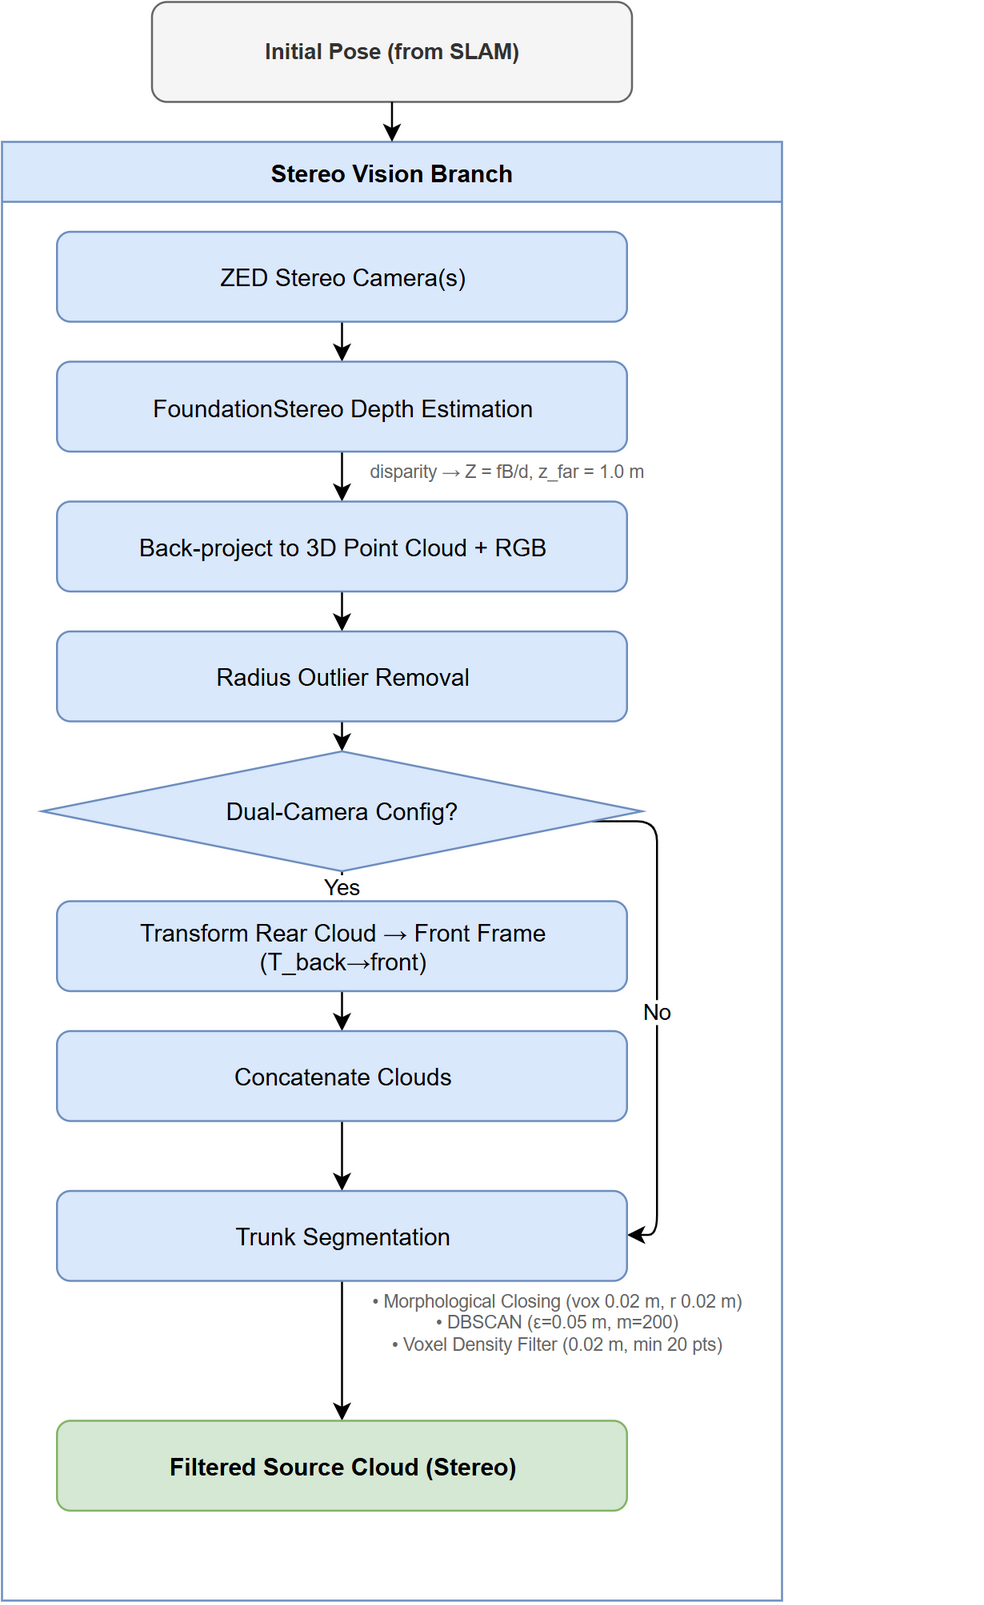
\includegraphics[width=0.65\linewidth]{4-precise-alignment/4-methodology/figures/pa-pipeline-stereo}
  \caption{Stereo vision preprocessing branch of the precise-alignment pipeline.
           Rectified image pairs from the ZED stereo camera(s) are processed
           through FoundationStereo depth estimation, back-projection, radius
           outlier removal, optional dual-camera fusion, and trunk segmentation
           to produce a filtered source point cloud passed to the shared GICP
           registration stage (\cref{fig:pa-pipeline-icp}).}
  \label{fig:pa-pipeline-stereo}
\end{figure}

\begin{figure}[htbp]
  \centering
  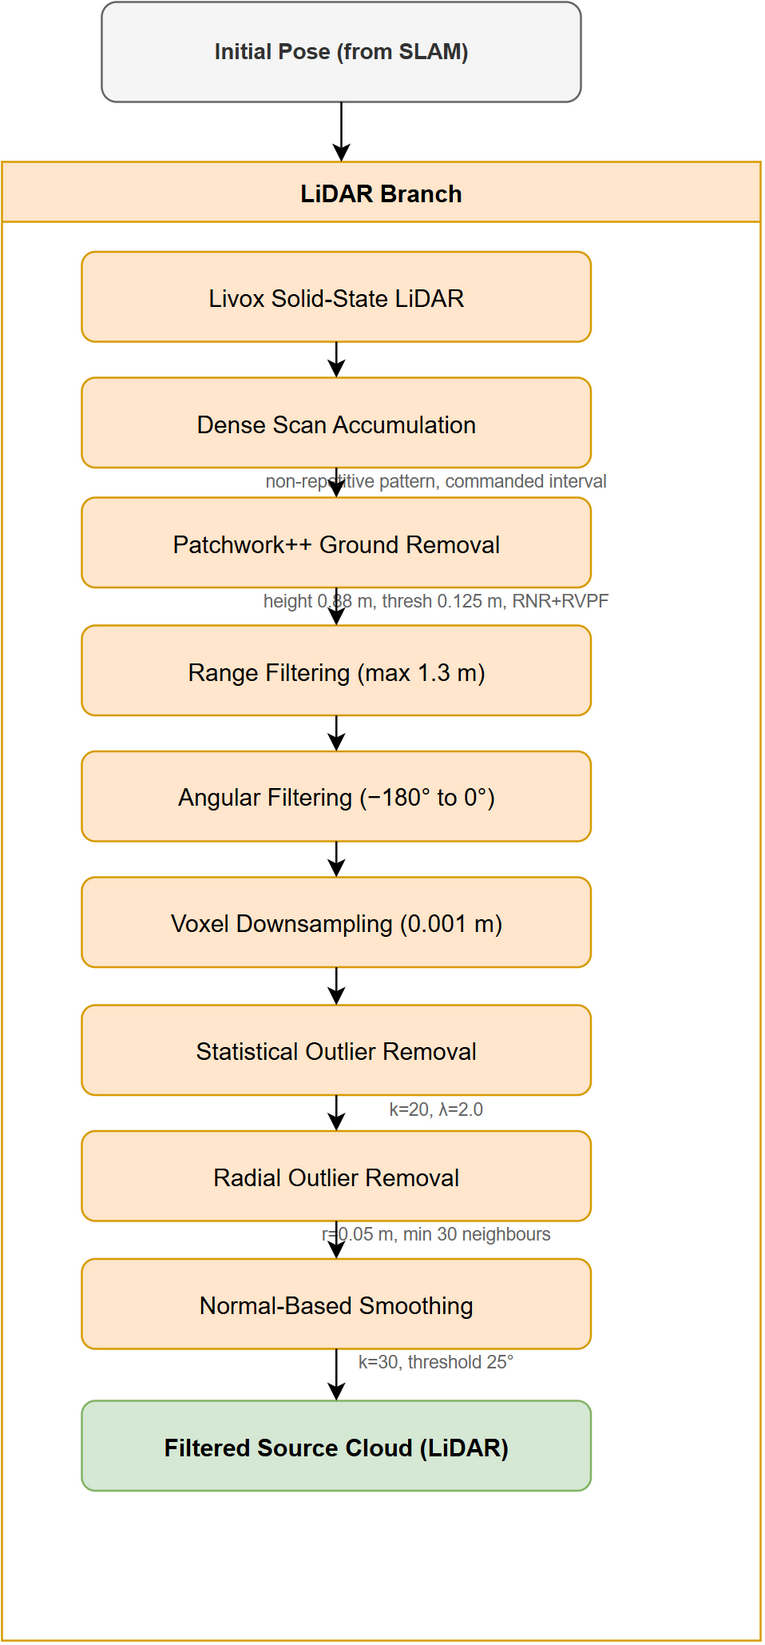
\includegraphics[width=0.65\linewidth]{4-precise-alignment/4-methodology/figures/pa-pipeline-lidar}
  \caption{LiDAR preprocessing branch of the precise-alignment pipeline. Dense
           scans from the Livox solid-state LiDAR are filtered through ground
           removal, statistical and angular outlier rejection, and normal-based
           smoothing to produce a filtered source point cloud passed to the
           shared GICP registration stage (\cref{fig:pa-pipeline-icp}).}
  \label{fig:pa-pipeline-lidar}
\end{figure}

\begin{figure}[htbp]
  \centering
  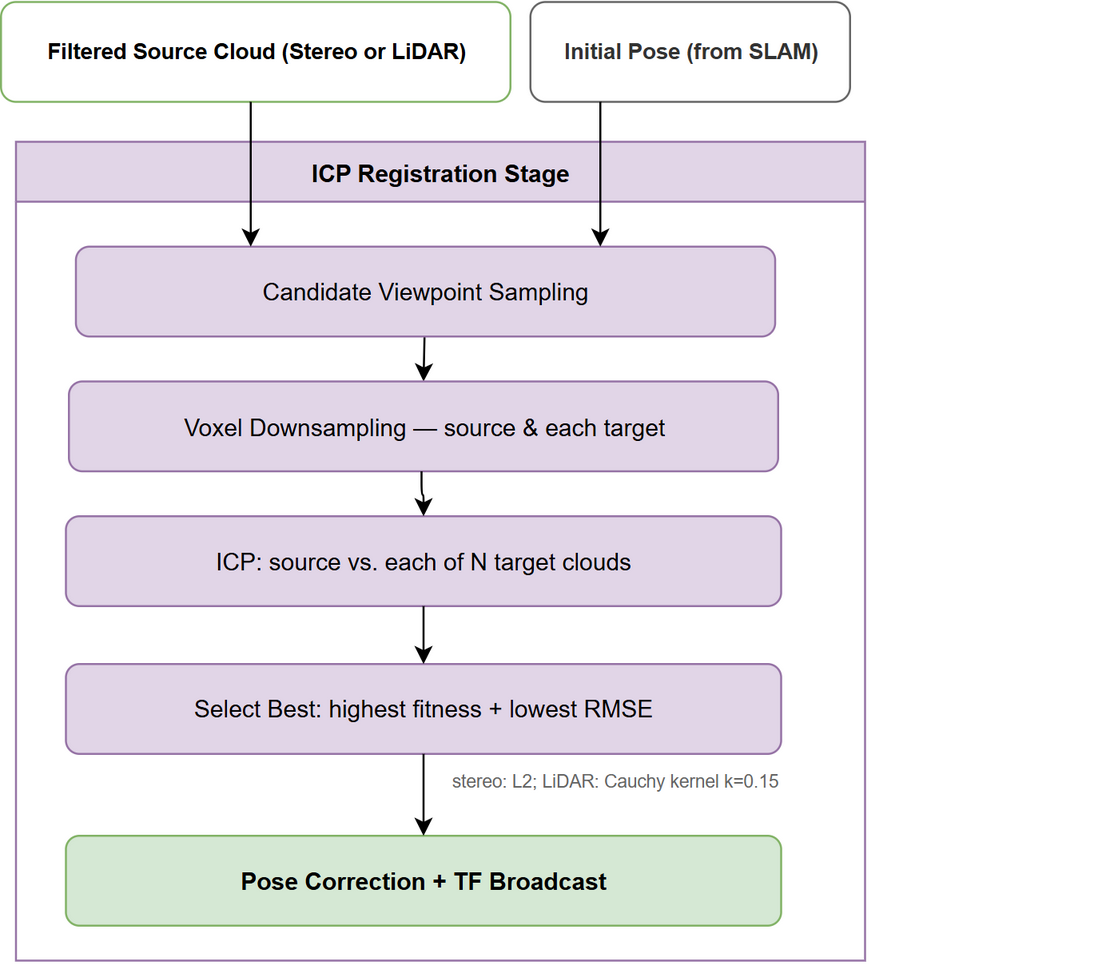
\includegraphics[width=0.85\linewidth]{4-precise-alignment/4-methodology/figures/pa-pipeline-icp}
  \caption{Shared GICP registration stage, common to both sensing modalities.
           A single target point cloud is extracted from the Gaussian mean
           positions of the 3DGS model; 35 perturbation hypotheses are sampled
           around the initial SLAM pose and each is registered via GICP against
           the extracted target cloud. The best-fitting result is used to correct
           the robot pose in the ROS~2 TF tree via the mechanism described in
           \cref{subsec:pa-pose-correction}.}
  \label{fig:pa-pipeline-icp}
\end{figure}

% ---------------------------------------------------------------
\subsection{Reference Model: 3D Gaussian Splatting}
\label{subsec:pa-reference-model}
% ---------------------------------------------------------------

The localisation target for both sensor modalities is a point cloud derived directly from the 3DGS model of the target vine. The construction of this model from SfM photogrammetry is described in \cref{subsec:system-context}; the present subsection addresses how it is used during localisation.

The 3DGS model is loaded once at initialisation. The target point cloud is constructed by extracting the mean positions of all Gaussian primitives stored in the model. Each primitive is parameterised by a mean $\boldsymbol{\mu}_i \in \mathbb{R}^3$, representing the centre of the volumetric Gaussian in world coordinates; collecting these centres across all $N$ primitives yields a single global point cloud $\{\boldsymbol{\mu}_i\}_{i=1}^{N}$ that captures the geometric structure of the reconstructed scene (see \cref{fig:pa-gaussian-splat-pointcloud}). This extraction is a direct read of the model parameters and requires no rendering pass, making it computationally simpler than viewpoint-dependent depth map synthesis and free of viewpoint-dependent artefacts that arise when projecting volumetric primitives onto an image plane.

Because the extracted cloud spans the full reconstructed scene, it is spatially cropped to a region of interest centred on the initial pose estimate before registration. This step retains only the local geometry relevant to the current alignment problem and discards distant or structurally irrelevant model points that would otherwise inflate correspondence search cost and introduce spurious matches. Following cropping, the target cloud may optionally be downsampled using a voxel grid filter to reduce point density and match the resolution of the incoming sensor source cloud, further reducing the computational cost of the subsequent registration step.

The resulting target cloud is constructed once per localisation query and reused across all perturbation hypotheses evaluated during ICP registration, as described in \cref{subsec:pa-icp-registration}. This avoids redundant reconstruction overhead and ensures a consistent geometric reference throughout the alignment procedure.

\begin{figure}[htbp]
  \centering
  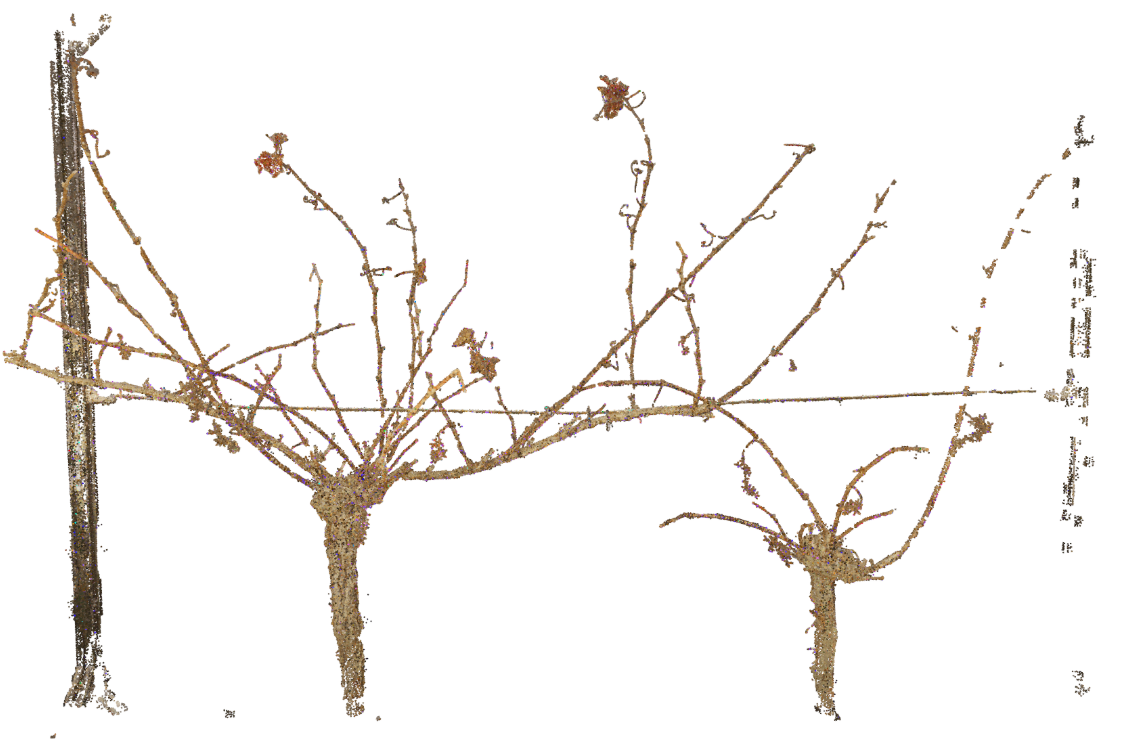
\includegraphics[width=0.85\linewidth]{4-precise-alignment/4-methodology/figures/pa-gaussian-splat-pointcloud}
  \caption{Point cloud derived from the 3DGS reference model of a dormant
           grapevine, constructed by extracting the mean positions
           $\boldsymbol{\mu}_i$ of all Gaussian primitives. Two vine trunks
           and the shared trellis wire are clearly resolved.}
  \label{fig:pa-gaussian-splat-pointcloud}
\end{figure}

% ---------------------------------------------------------------
\subsection{Stereo Vision Pipeline}
\label{subsec:pa-stereo-pipeline}
% ---------------------------------------------------------------

The stereo vision pipeline converts raw rectified image pairs from the ZED stereo camera into a filtered point cloud of the vine trunk, for registration against the 3DGS target described in \cref{subsec:pa-reference-model}. The pipeline proceeds through three sequential stages: dense depth estimation from the stereo pair, optional fusion of point clouds from a laterally offset camera pair, and trunk segmentation to remove non-structural points. The output is passed directly to the shared ICP registration stage described in \cref{subsec:pa-icp-registration}.

\subsubsection{Depth Estimation}
\label{subsubsec:pa-depth-estimation}

Dense depth estimation is performed using FoundationStereo~\cite{wenFoundationStereoZeroShot2025},
a stereo foundation model that produces disparity maps with strong zero-shot generalisation across sensor configurations and scene types (see \cref{subsec:stereo-depth} for a description of the model and its benchmark performance).
The \texttt{23-51-11} checkpoint is used without any fine-tuning; inference is applied in a purely zero-shot manner.
FoundationStereo is applied to rectified image pairs from the ZED Mini stereo camera. Prior to inference, the input images are downscaled by a factor of 0.7 relative to the original sensor resolution.
This factor was determined empirically: the largest input resolution that can be processed without exceeding available GPU memory was identified, and a 20\,\% safety margin was applied, yielding the 0.7 scale factor.

The disparity map produced by FoundationStereo is converted to metric depth via the standard pinhole relation (see \cref{subsec:stereo-depth}):
%
\begin{equation}
    Z = \frac{f \cdot B}{d},
\end{equation}
%
where $Z$ is the metric depth, $f$ is the focal length of the rectified camera model, $B$ is the stereo baseline, and $d$ is the estimated disparity at each pixel. A far-clip distance of $z_\mathrm{far} = 1.0$\,m is applied to discard depth estimates beyond the typical operating range between the robot and the target vine.
% TODO: review justification: z_far = 1.0 m reflects the close-range operating distance in the vineyard row; review against actual deployment geometry
Points with depth below a minimum threshold are also discarded to suppress artefacts close to the camera aperture.

Each pixel for which a valid depth estimate is available is back-projected into a three-dimensional point in the camera frame, using the corresponding RGB values to produce a coloured point cloud. A radius outlier removal filter is subsequently applied to eliminate sparse, isolated points that are not part of any coherent surface.

\subsubsection{Dual-Camera Point Cloud Fusion}
\label{subsubsec:pa-dual-camera}

The system supports an optional dual-camera configuration in which a second ZED stereo camera (ZED~2) is mounted alongside the primary camera (ZED~1) on the vine-facing side of the robot platform, approximately 30\,cm laterally offset with no rotation between the two units. Both cameras are directed toward the same face of the vine structure, producing overlapping point clouds from slightly different lateral vantage points.

This configuration serves two complementary purposes. First, the lateral offset provides marginally different viewing angles of the vine surface, yielding a denser and more representative composite point cloud than either camera alone. Second, points in the shared field of view are observed from two independent viewpoints and therefore accumulate higher local density after concatenation; this is passively exploited by the downstream density-sensitive filters described in \cref{subsubsec:pa-trunk-segmentation}, which preferentially retain the denser overlap region over sparse peripheral returns. No explicit consistency-based outlier rejection is applied in the current implementation. Flagging depth estimates that appear in one cloud but are absent or inconsistent in the other would represent a more deliberate exploitation of the overlap, and remains a potential avenue for improvement. This stands in contrast to a configuration in which the two cameras view the vine from opposite or widely separated directions, where each cloud would have to be accepted independently with no means of cross-validation.

The extrinsic relationship between the two cameras is expressed as a rigid transform from the secondary camera frame (ZED~2) to the primary camera frame (ZED~1). Given the transform from the primary camera to a common reference frame, $T_{\mathrm{cam1} \to \mathrm{ref}}$, and the corresponding transform from the secondary camera, $T_{\mathrm{cam2} \to \mathrm{ref}}$, the inter-camera transform is computed as:
%
\begin{equation}
    T_{\mathrm{cam2} \to \mathrm{cam1}} = T_{\mathrm{cam1} \to \mathrm{ref}}^{-1} \cdot T_{\mathrm{cam2} \to \mathrm{ref}}.
    \label{eq:dual-camera-extrinsic}
\end{equation}
%
The secondary camera point cloud is transformed into the primary camera frame using $T_{\mathrm{cam2} \to \mathrm{cam1}}$, and the two clouds are concatenated (\cref{fig:pa-dual-camera}). Since both cameras share the same pointing direction, the rotation component of $T_{\mathrm{cam2} \to \mathrm{cam1}}$ is the identity in the nominal configuration, reducing the transform to a pure lateral translation of approximately 30\,cm.

\begin{figure}[htbp]
  \centering
  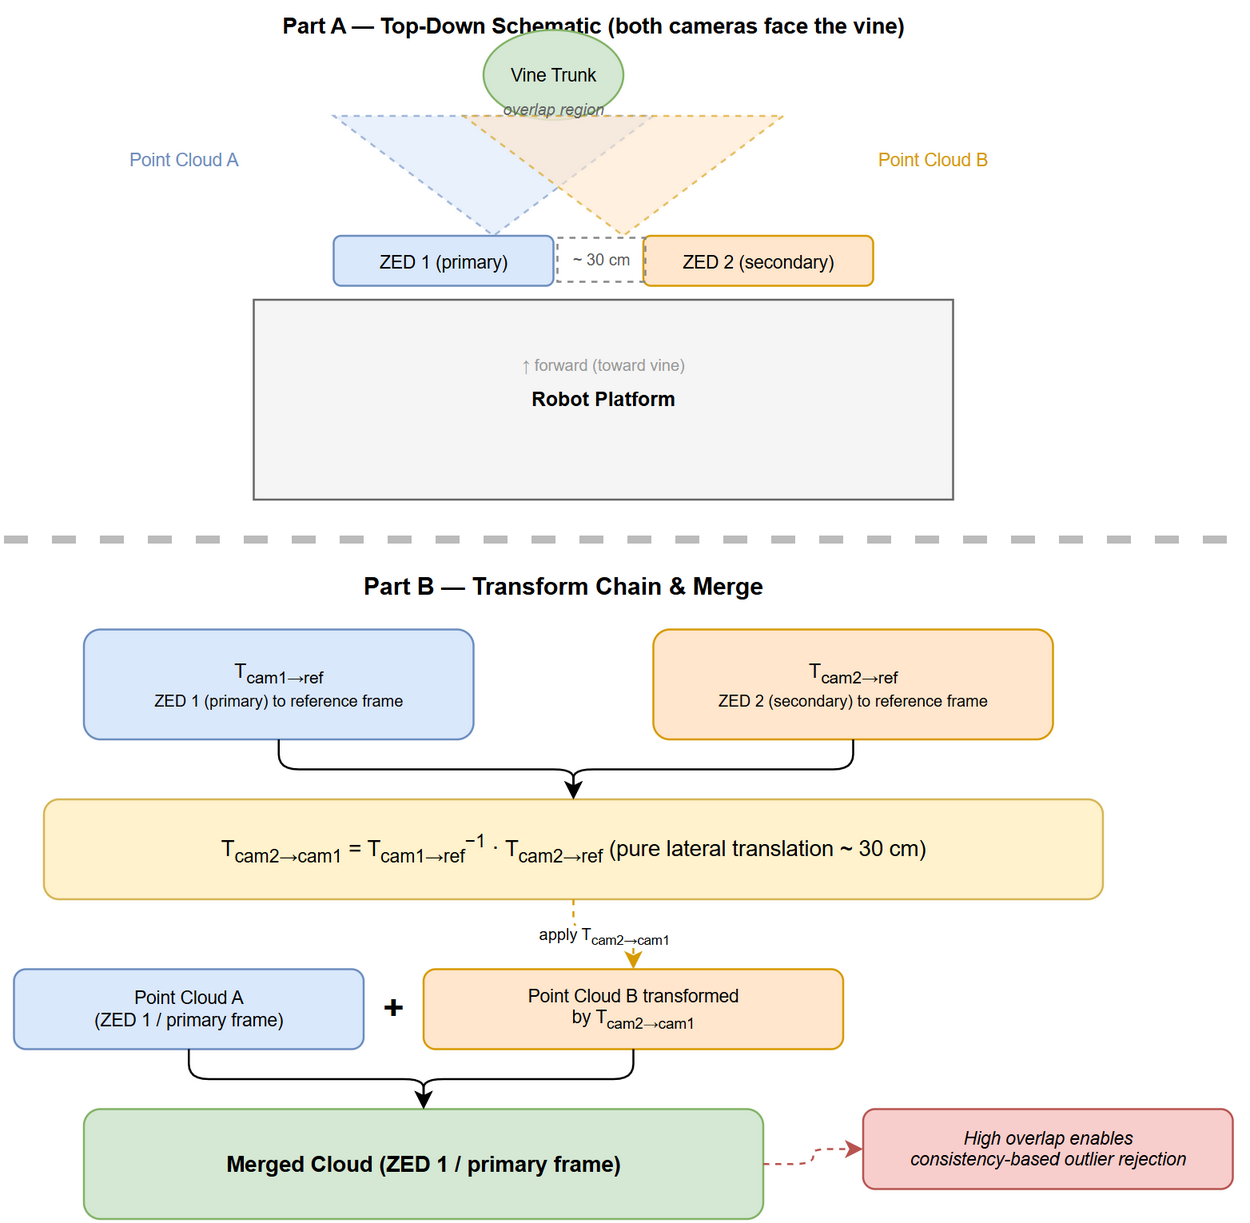
\includegraphics[width=\linewidth]{4-precise-alignment/4-methodology/figures/pa-dual-camera}
  \caption{Dual-camera point cloud fusion. Both ZED cameras are mounted side by side
           on the vine-facing side of the robot, approximately 30\,cm apart with no
           rotation between them, and directed toward the same face of the vine (Part~A).
           The secondary camera's point cloud is transformed into the primary camera
           frame using $T_{\mathrm{cam2} \to \mathrm{cam1}}$ (\cref{eq:dual-camera-extrinsic}),
           and the two clouds are concatenated (Part~B). The resulting overlap region
           accumulates higher local point density, which is passively exploited by the
           downstream density-sensitive filters in the trunk segmentation stage.}
  \label{fig:pa-dual-camera}
\end{figure}

\subsubsection{Trunk Segmentation}
\label{subsubsec:pa-trunk-segmentation}

A custom trunk segmentation pipeline developed for this work is applied to the merged (or single-camera) point cloud to isolate the vine trunk from background vegetation, noise, and ground returns; the three sequential stages are summarised in \cref{fig:pa-trunk-segmentation}.

\begin{figure}[htbp]
  \centering
  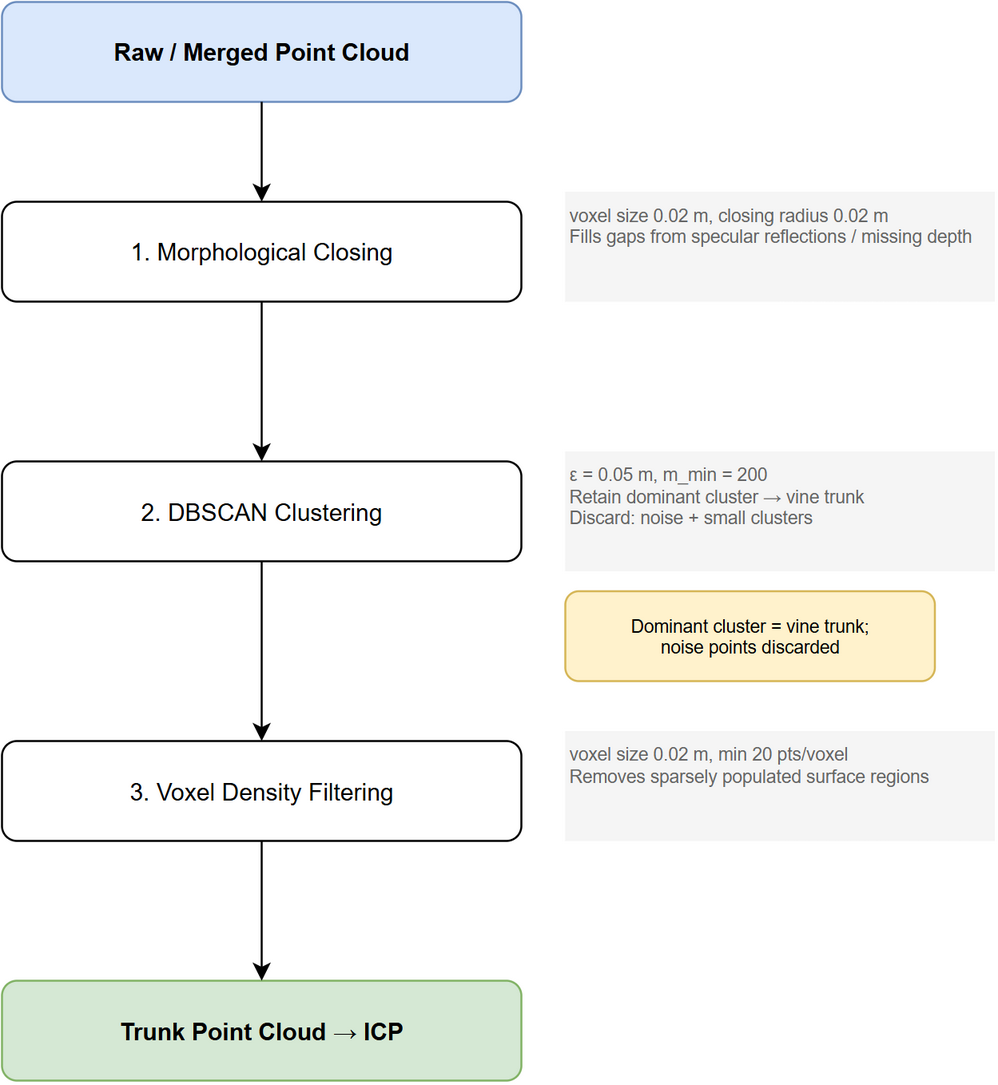
\includegraphics[width=0.75\linewidth]{4-precise-alignment/4-methodology/figures/pa-trunk-segmentation}
  \caption{Stereo trunk segmentation pipeline. The merged point cloud passes through
           three sequential stages (morphological closing, DBSCAN clustering, and
           voxel density filtering) to isolate the vine trunk from background
           vegetation, ground returns, and noise.}
  \label{fig:pa-trunk-segmentation}
\end{figure}

The pipeline comprises three sequential stages. Prior to the first stage, the combined cloud is capped at 600,000 points by random subsampling, bounding the worst-case computation time independently of sensor resolution or accumulation duration.
% TODO: review whether 600,000 is the tightest practical cap; review against observed input sizes

\textbf{Morphological closing.} A voxel-based morphological closing operation fills gaps in the trunk surface caused by specular reflections or missing depth estimates. The input cloud is voxelised at a resolution of 0.02\,m, and a spherical closing kernel of radius 0.02\,m is applied.
% TODO: review parameter justification: voxel size 0.02 m and closing radius 0.005 m were selected to bridge typical surface gaps in stereo depth reconstructions of vine bark; review against observed gap statistics

\textbf{DBSCAN clustering.} Density-Based Spatial Clustering of Applications with Noise (DBSCAN)~\cite{esterDensityBasedAlgorithmDiscovering1996}
partitions the closed point cloud into spatially coherent clusters. DBSCAN groups points whose neighbourhood within radius $\varepsilon$ contains at least $m_\mathrm{min}$ neighbouring points, classifying the remainder as noise. With $\varepsilon = 0.05$\,m and $m_\mathrm{min} = 200$,
% TODO: review parameter justification: eps = 0.05 m reflects the typical inter-point spacing at vine-trunk distances; min_samples = 200 was chosen to reject small noise clusters while retaining the dominant trunk; review against cloud density statistics
the dominant cluster, corresponding to the vine trunk, is retained, and all other clusters and noise points are discarded.

\textbf{Voxel density filtering.} The retained cluster is passed through a voxel density filter that partitions the cloud into voxels of side length 0.02\,m and discards any voxel containing fewer than 20 points.
% TODO: review parameter justification: voxel size 0.02 m and min count 20 eliminate residual sparse regions that survived clustering; review against observed point density at typical vine-to-sensor distances
This step removes sparsely populated surface regions whose geometric contribution to the ICP objective would otherwise be disproportionate to their informational content.
\Cref{fig:pa-stereo-pointcloud-processing} illustrates the effect of the full stereo preprocessing pipeline on a representative observation.

\begin{figure}[htbp]
  \centering
  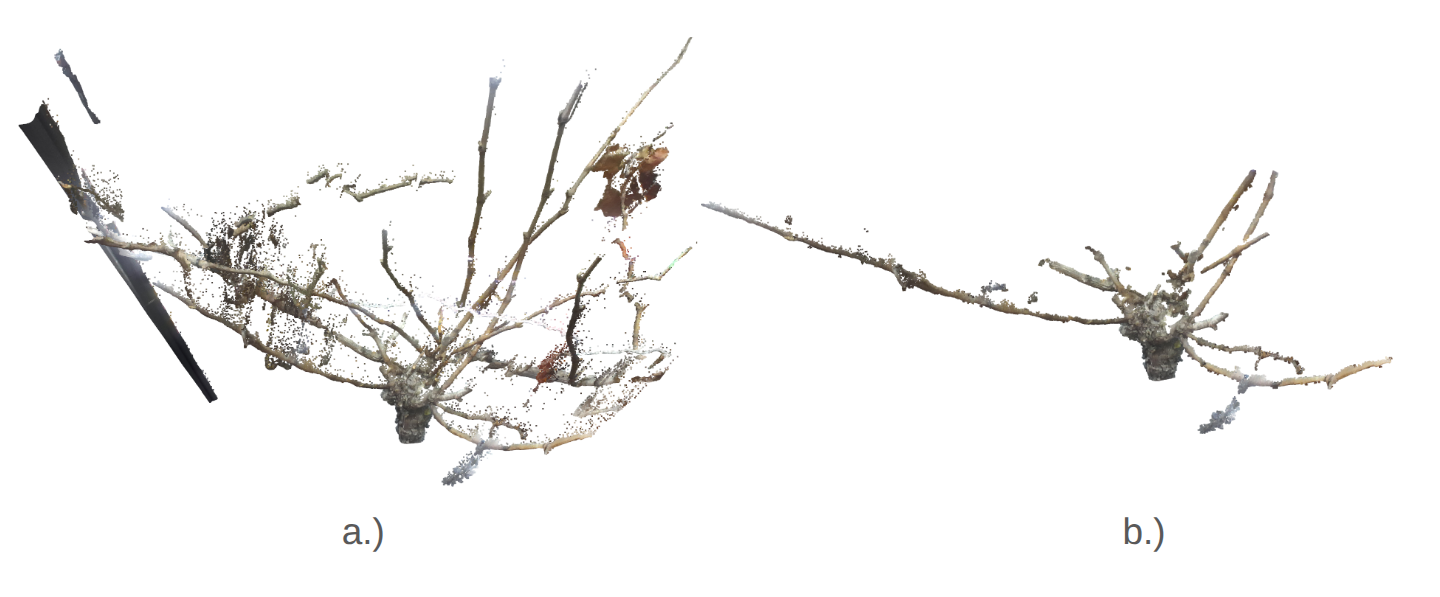
\includegraphics[width=\linewidth]{4-precise-alignment/4-methodology/figures/pa-stereo-pointcloud-processing}
  \caption{Stereo point cloud before and after preprocessing.
           (a) The raw back-projected point cloud prior to filtering, exhibiting
           significant noise, non-structural returns, and artefacts.
           (b) The filtered point cloud following the full trunk segmentation
           pipeline, retaining only the vine trunk geometry forwarded to GICP
           registration.}
  \label{fig:pa-stereo-pointcloud-processing}
\end{figure}

The parameters for the stereo preprocessing pipeline are summarised in \cref{tab:pa-stereo-params}.

\begin{table}[htbp]
  \centering
  \caption{Stereo vision pipeline parameters.}
  \label{tab:pa-stereo-params}
  \begin{tabularx}{\textwidth}{l l X}
    \toprule
    \textbf{Parameter} & \textbf{Value} & \textbf{Description} \\
    \midrule
    Downscale factor          & 0.7        & Input image downscale factor for FoundationStereo inference; empirically derived with a 20\,\% GPU memory safety margin \\
    $z_\mathrm{far}$          & 1.0\,m     & Far-clip depth; points beyond this distance are discarded \\
    Closing voxel size        & 0.02\,m    & Voxel resolution for the morphological closing operation \\
    Closing radius            & 0.02\,m    & Spherical kernel radius for the closing operator \\
    DBSCAN $\varepsilon$      & 0.05\,m    & Neighbourhood radius for cluster membership \\
    DBSCAN $m_\mathrm{min}$   & 200        & Minimum point count to form a core cluster \\
    Density filter voxel size & 0.02\,m    & Voxel size for the density filtering stage \\
    Density filter min count  & 20         & Minimum points per voxel \\
    Input point cap           & 600\,000   & Maximum points admitted to the segmentation pipeline \\
    \bottomrule
  \end{tabularx}
  % TODO: verify all parameter values and add justifications
\end{table}

% ---------------------------------------------------------------
\subsection{LiDAR Pipeline}
\label{subsec:pa-lidar-pipeline}
% ---------------------------------------------------------------

The LiDAR pipeline converts raw scans from the LiDAR into a filtered point cloud of the vine structure, ready for registration. The pipeline proceeds through three stages: dense scan accumulation to build a spatially rich input cloud, ground plane removal using Patchwork++, and sequential geometric filtering. The output is dispatched to the shared ICP registration stage described in \cref{subsec:pa-icp-registration}.

\subsubsection{Dense Scan Accumulation}
\label{subsubsec:pa-dense-accumulation}

The Livox Mid-360 employs a non-repetitive scanning pattern in which, unlike a conventional spinning LiDAR, the scan lines do not repeat on a fixed cycle. Consequently, a single frame provides sparse and unevenly distributed coverage of the target. A custom dense-mapper ROS~2 node~\cite{macenskiRobotOperatingSystem2022} developed for this work accumulates multiple consecutive scans over a commanded time interval, concatenating their returns into a single dense point cloud. In the present work, the accumulation interval is set to 25\,s, yielding approximately 4.4--4.6 million raw points per acquisition. This raw cloud is subsequently reduced to approximately 100\,000 points by the multi-stage filtering pipeline described in \cref{subsubsec:pa-lidar-processing}. Over the 25\,s interval, the non-repetitive pattern achieves high fill-factor coverage of the scene within the sensor's field of view, producing a point cloud with spatial density comparable to that of a multi-return spinning LiDAR.

\subsubsection{Ground Segmentation}
\label{subsubsec:pa-ground-segmentation}

The accumulated point cloud includes returns from the vineyard floor. Because the 3DGS reference model contains little ground geometry, these returns have no counterparts in the target cloud; retaining them introduces spurious correspondences during ICP that bias the registration away from the correct alignment. Ground plane removal is therefore applied to increase the similarity between the source and target clouds. Ground removal is performed using Patchwork++~\cite{leePatchworkFastRobust2022},
an incremental ground segmentation algorithm that models the ground surface as a set of concentric annular patches and applies region-wise plane fitting with outlier rejection. The method is robust to uneven terrain and does not require a flat-ground assumption.

The parameters used in this work are as follows. The sensor height above the ground surface is set to 0.88\,m,
consistent with the physical mounting position of the Livox sensor on the robot platform. The distance threshold for classifying a point as ground is 0.125\,m.
% TODO: review: distance threshold chosen to accommodate minor terrain irregularities; review against observed ground surface roughness
The seed threshold for initialising planar patches is 0.5\,m, and three plane-fitting iterations are applied per patch.
% TODO: review seed threshold justification
The processing range is bounded to 0.1--3.0\,m to discard returns either too close to the sensor aperture or beyond the typical vine operating distance. 

\subsubsection{Point Cloud Processing}
\label{subsubsec:pa-lidar-processing}

Following ground removal, the non-ground point cloud is passed through a custom multi-stage filtering pipeline developed for this work; the six sequential stages are illustrated in \cref{fig:pa-lidar-filtering}.

\begin{figure}[htbp]
  \centering
  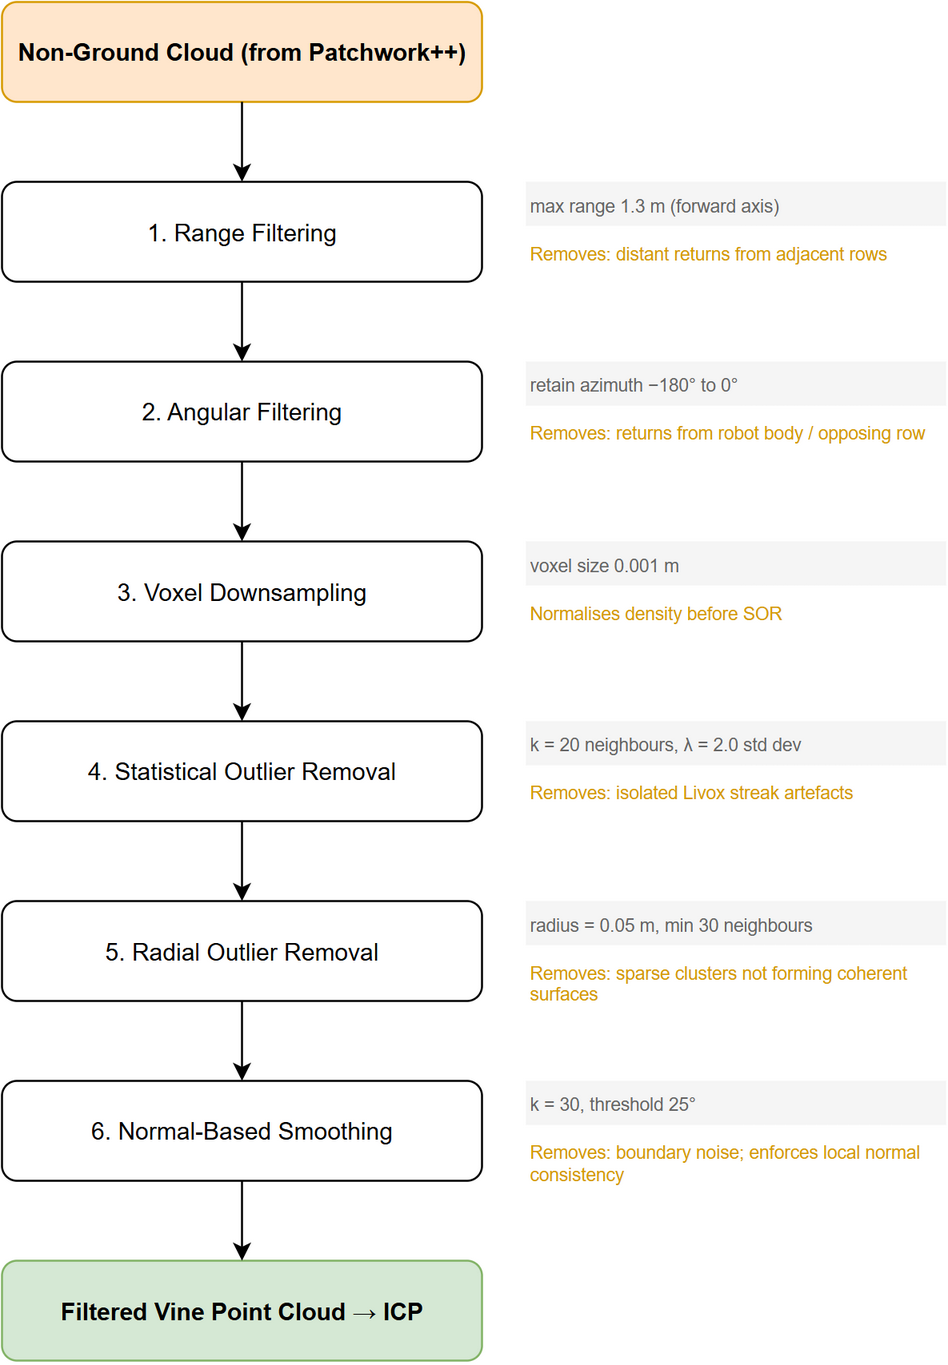
\includegraphics[width=0.75\linewidth]{4-precise-alignment/4-methodology/figures/pa-lidar-filtering}
  \caption{LiDAR point cloud filtering pipeline. Six sequential stages process the
           non-ground Livox cloud to isolate vine wood structure prior to ICP
           registration.}
  \label{fig:pa-lidar-filtering}
\end{figure}

The six sequential stages are described below.

\textbf{Range filtering.} Points beyond a maximum range of 1.3\,m from the sensor are discarded. This restricts the cloud to the area of the target vine, removing distant returns from adjacent rows and structures that do not exist in the 3DGS reference model.

\textbf{Angular filtering.} Points in the azimuthal range from $-180^{\circ}$ to $0^{\circ}$ are retained; returns outside this half-space are discarded.
This step exploits the known mounting orientation of the Livox sensor to exclude returns from the robot body and from the vineyard row that the robot is not currently targeting.

\textbf{Voxel downsampling.} The angular-filtered point cloud is downsampled using a voxel grid filter with voxel side length 0.001\,m. This normalises point density before subsequent filtering stages, ensuring that the statistical outlier removal threshold operates on a spatially uniform cloud rather than being biased by density variations inherent to the non-repetitive scan pattern.

\textbf{Statistical outlier removal.} Each point is evaluated against its $k$-nearest neighbourhood; points whose mean neighbour distance exceeds the population mean by more than $\lambda$ standard deviations are classified as outliers and removed. With $k = 20$ and $\lambda = 2.0$, Operating on the voxel-downsampled cloud ensures that the mean-plus-$2\sigma$ threshold targets outliers rather than points in naturally sparse scan regions.

\textbf{Radial outlier removal.} A spherical neighbourhood of radius 0.05\,m around each point is examined; points with fewer than 30 neighbours within that radius are discarded.
This pass targets point clusters that are spatially consistent at the individual-point level but are too isolated to form part of a coherent surface.

\textbf{Normal-based smoothing.} Surface normals are estimated for each point from its 30 nearest neighbours. Points whose estimated normal deviates by more than $25^{\circ}$ from the local consensus are discarded, enforcing normal consistency across the retained surface. This smoothing pass reduces boundary effects and the influence of surface noise on the ICP correspondence stage.

The parameters for the LiDAR preprocessing pipeline are summarised in \cref{tab:pa-lidar-params}.

\begin{table}[htbp]
  \centering
  \caption{LiDAR pipeline parameters.}
  \label{tab:pa-lidar-params}
  \begin{tabularx}{\textwidth}{l l X}
    \toprule
    \textbf{Parameter} & \textbf{Value} & \textbf{Description} \\
    \midrule
    \multicolumn{3}{l}{\textit{Patchwork++ ground segmentation}} \\
    \midrule
    Sensor height          & 0.88\,m        & Mounting height of the Livox sensor above the ground \\
    Distance threshold     & 0.125\,m       & Maximum deviation from the fit plane to be classified as ground \\
    Seed threshold         & 0.5\,m         & Height threshold for initial ground seed selection \\
    Fitting iterations     & 3              & Number of plane-fitting iterations per annular patch \\
    Processing range       & 0.1--3.0\,m    & Minimum and maximum range included in ground estimation \\
    RNR                    & Enabled        & Ring-wise Normal-based Removal \\
    RVPF                   & Enabled        & Ring-wise Vertical Point Filtering \\
    \midrule
    \multicolumn{3}{l}{\textit{Point cloud filtering}} \\
    \midrule
    Range filter max range              & 1.3\,m                    & Maximum range from sensor along the forward axis \\
    Angular filter range                & $-180^{\circ}$ to $0^{\circ}$ & Retained azimuthal range \\
    Voxel downsample size               & 0.001\,m                  & Voxel side length for density normalisation prior to SOR \\
    Statistical outlier $k$             & 20                        & Neighbourhood size for statistical outlier removal \\
    Statistical outlier $\lambda$       & 2.0                       & Standard deviation multiplier for the outlier threshold \\
    Radial outlier radius               & 0.05\,m                   & Neighbourhood radius for radial outlier removal \\
    Radial outlier min neighbours       & 30                        & Minimum neighbours within the search radius \\
    Normal smooth $k$                   & 30                        & Neighbourhood size for normal estimation \\
    Normal smooth threshold             & $25^{\circ}$              & Maximum normal deviation for smoothing-stage retention \\
    \bottomrule
  \end{tabularx}
  % TODO: verify all parameter values and add justifications
\end{table}

% ---------------------------------------------------------------
\subsection{ICP Registration Against the 3DGS Model}
\label{subsec:pa-icp-registration}
% ---------------------------------------------------------------

Both the stereo and LiDAR preprocessing branches deliver a filtered source point cloud to a shared Generalised ICP (GICP) registration module, developed for this work, which aligns the sensor observation against a fixed target point cloud extracted from the 3DGS model. The registration procedure is as follows.

\textbf{(a) Initial pose.} The initial pose estimate, obtained from the SLAM system (\cref{sec:slam-methodology}), is represented as a $4 \times 4$ homogeneous transformation matrix in $SE(3)$, encoding the rotation and translation of the robot base in the global frame.

\textbf{(b) Target cloud construction.} A single target point cloud is constructed once from the Gaussian means of the 3DGS model, as described in \cref{subsec:pa-reference-model}..

\textbf{(c) Neighbourhood perturbation.} To mitigate sensitivity to the accuracy of the initial SLAM pose, the pipeline generates N candidate initial poses by applying small rigid-body perturbations to the initial estimate $T_0$. Each perturbed pose $T_k$ is formed by right-multiplying $T_0$ with a perturbation matrix $\Delta T_k$:
%
\begin{equation}
    T_k = T_0 \cdot \Delta T_k, \qquad k = 0, \ldots, N-1.
    \label{eq:perturbation}
\end{equation}
%
Right-multiplication ensures that perturbations are applied in the body frame of the robot, so that translations and rotations act along the robot's local axes rather than the global frame axes. The N hypotheses are organised into five groups according to the structure of $\Delta T_k$, as summarised in \cref{tab:pa-perturbation-groups}. The perturbation magnitudes $\delta_t$ (translation) and $\delta_r$ (rotation) are configurable parameters whose values are reported in \cref{tab:pa-icp-params}. The perturbation scheme and subsequent hypothesis selection are illustrated in \cref{fig:pa-icp-candidates}.

\begin{table}[htbp]
  \centering
  \caption{Perturbation hypothesis groups. Each group defines a class of rigid-body perturbation applied to the initial pose to generate candidate starting points for GICP registration.}
  \label{tab:pa-perturbation-groups}
  \begin{tabularx}{\textwidth}{l l X}
    \toprule
    \textbf{Group} & \textbf{Count} & \textbf{Description} \\
    \midrule
    Orig & 1  & Nominal (unperturbed) pose; $\Delta T_0 = I_{4\times4}$ \\
    A    & 6  & Axis-aligned translations along $\pm x$, $\pm y$, $\pm z$ at half the nominal magnitude ($\delta_t / 2$) \\
    B    & 4  & Cardinal-direction translations in the horizontal plane ($+x$, $-x$, $+y$, $-y$) at the full nominal magnitude ($\delta_t$) \\
    C    & 12 & Compound perturbations combining a diagonal horizontal translation ($\delta_t$) with a yaw rotation ($\pm \delta_r$), sampling the four diagonal directions (NE, SE, SW, NW) with both positive and negative yaw \\
    E    & 12 & Rotation-only perturbations sweeping roll, pitch, and yaw about each axis at both half-magnitude ($\delta_r / 2$) and full magnitude ($\delta_r$), with positive and negative signs \\
    \midrule
    \textbf{Total} & \textbf{35} & \\
    \bottomrule
  \end{tabularx}
\end{table}

\begin{figure}[htbp]
  \centering
  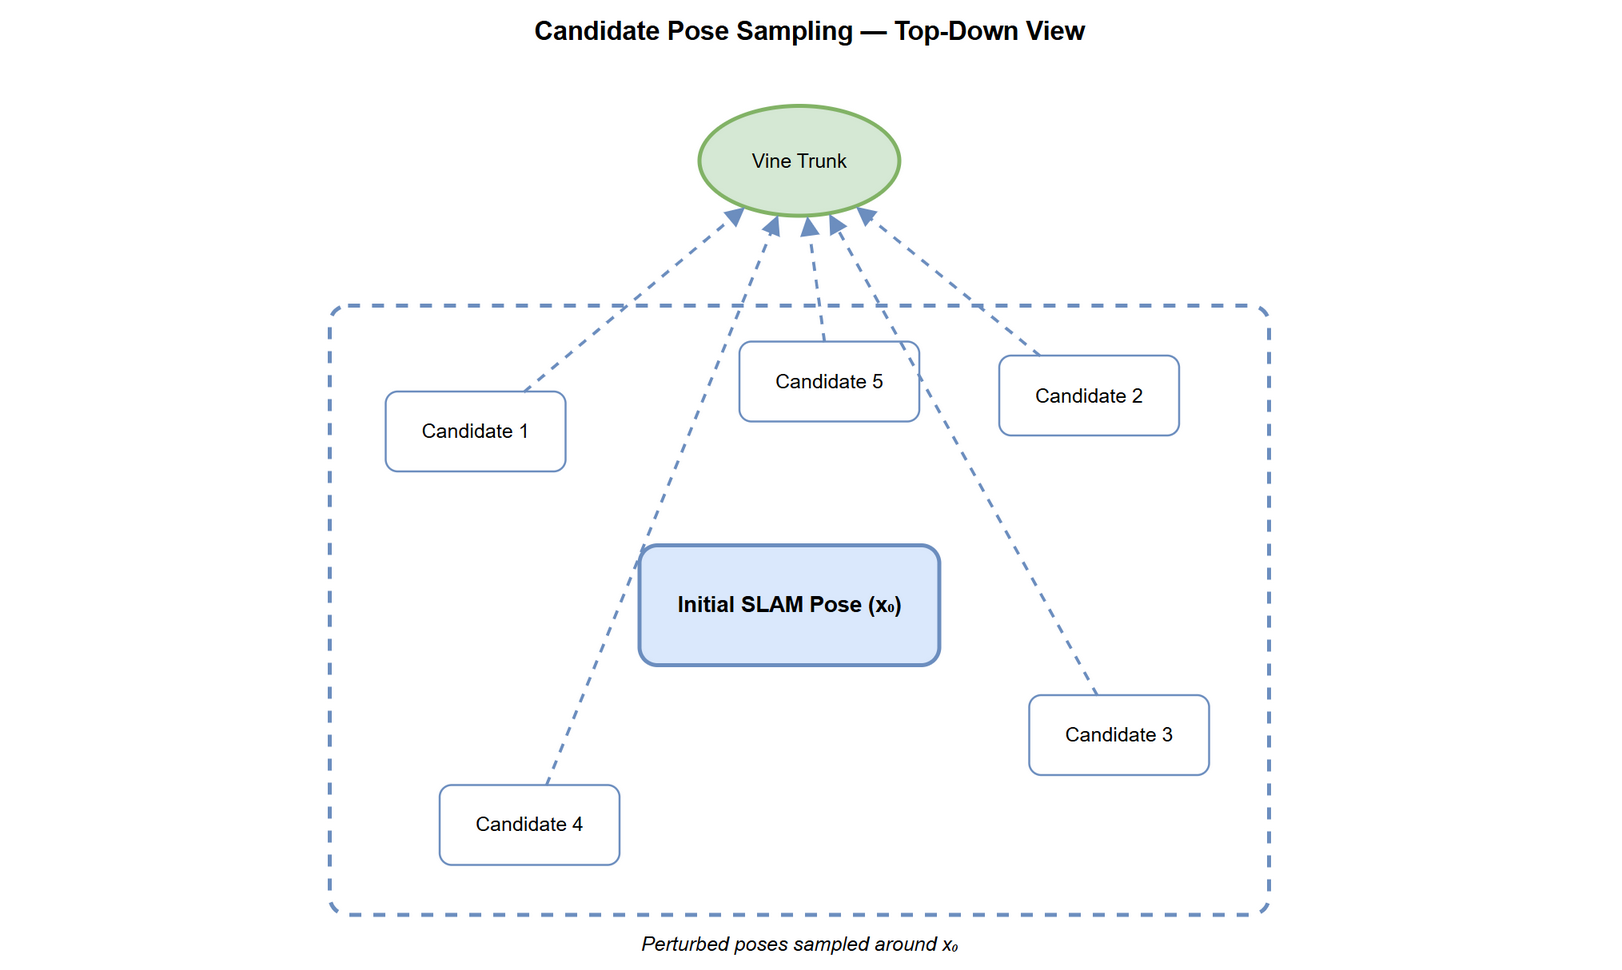
\includegraphics[width=\linewidth]{4-precise-alignment/4-methodology/figures/pa-icp-candidates}
  \caption{Candidate pose sampling scheme (top-down view). Thirty-five candidate poses are generated
           by applying structured rigid-body perturbations (Orig and Groups~A, B, C,~and~E; \cref{tab:pa-perturbation-groups})
           to the initial SLAM pose; each hypothesis is registered independently against the
           target point cloud extracted from the 3DGS model. The hypothesis achieving the highest
           fitness score above the acceptance threshold (lowest RMSE as a tiebreaker) is selected
           as the final alignment.}
  \label{fig:pa-icp-candidates}
\end{figure}

\textbf{(d) Downsampling.} Both the source cloud and the target cloud are downsampled using a voxel grid filter with voxel side length $v = 0.0075$\,m. The target cloud may have been pre-downsampled during construction (see \cref{subsec:pa-reference-model}); the additional voxel filter ensures a consistent resolution across registration runs. This step reduces the computational cost of each GICP iteration while retaining sufficient geometric detail for convergence.

\textbf{(e) GICP.} GICP~\cite{segalGeneralizedICP2009} is run between the downsampled source cloud and the downsampled target cloud using the \texttt{registration\_generalized\_icp} function from Open3D~\cite{zhouOpen3DModernLibrary2018}. Unlike standard point-to-point ICP, GICP models local surface structure by estimating covariance matrices in the neighbourhood of each point in both the source and target clouds, using a hybrid KD-tree neighbourhood search. The generalised objective incorporates these covariances to perform an effective plane-to-plane alignment, making it more robust to incorrect correspondences than the point-to-point formulation~\cite{segalGeneralizedICP2009}. Each of the 35 perturbed initial poses is used as the starting transformation for an independent GICP run. Each run applies a two-phase graduated loss strategy with an accumulated rotation constraint, as described below; the governing parameters are summarised in \cref{tab:pa-icp-params}.

\textbf{(f) Hypothesis selection.} After all 35 GICP runs complete, hypotheses with a fitness score below a threshold of 0.8 are rejected, where fitness is defined as the ratio of accepted correspondences to total source points. A fitness score of 0.8 requires that at least 80\% of the source points find a geometrically consistent correspondence in the target cloud, ensuring that the accepted alignment is supported by the majority of the observed structure rather than a minority subset. Among the remaining hypotheses, the result with the highest fitness score is selected as the final alignment, with the lowest RMSE used as a tiebreaker when fitness scores are equal.

The output of the registration stage is a result object containing the estimated transformation matrix, the fitness score, the point-to-point RMSE, and the accepted correspondence set.

\subsubsection*{Graduated Loss Strategy and Rotation Constraint}
\label{subsubsec:pa-graduated-icp}

Applying a single robust loss function throughout an ICP run creates a tension between two competing requirements. In early iterations, the source and target clouds are poorly aligned, so most point correspondences carry large residuals regardless of their geometric validity; aggressive outlier rejection at this stage can discard informative correspondences from thin structures such as branches and support wires, impeding convergence. Once broad alignment is achieved, the residuals that remain large arise from genuinely poor correspondences (edge noise, structural ambiguity), and strong suppression is desirable to lock the solution onto reliable inlier correspondences. A graduated loss strategy addresses this tension by using a permissive loss in the first phase and switching to an aggressive loss in the second. The complete constrained registration loop is illustrated in \cref{fig:pa-graduated-icp}.

\begin{figure}[htbp]
  \centering
  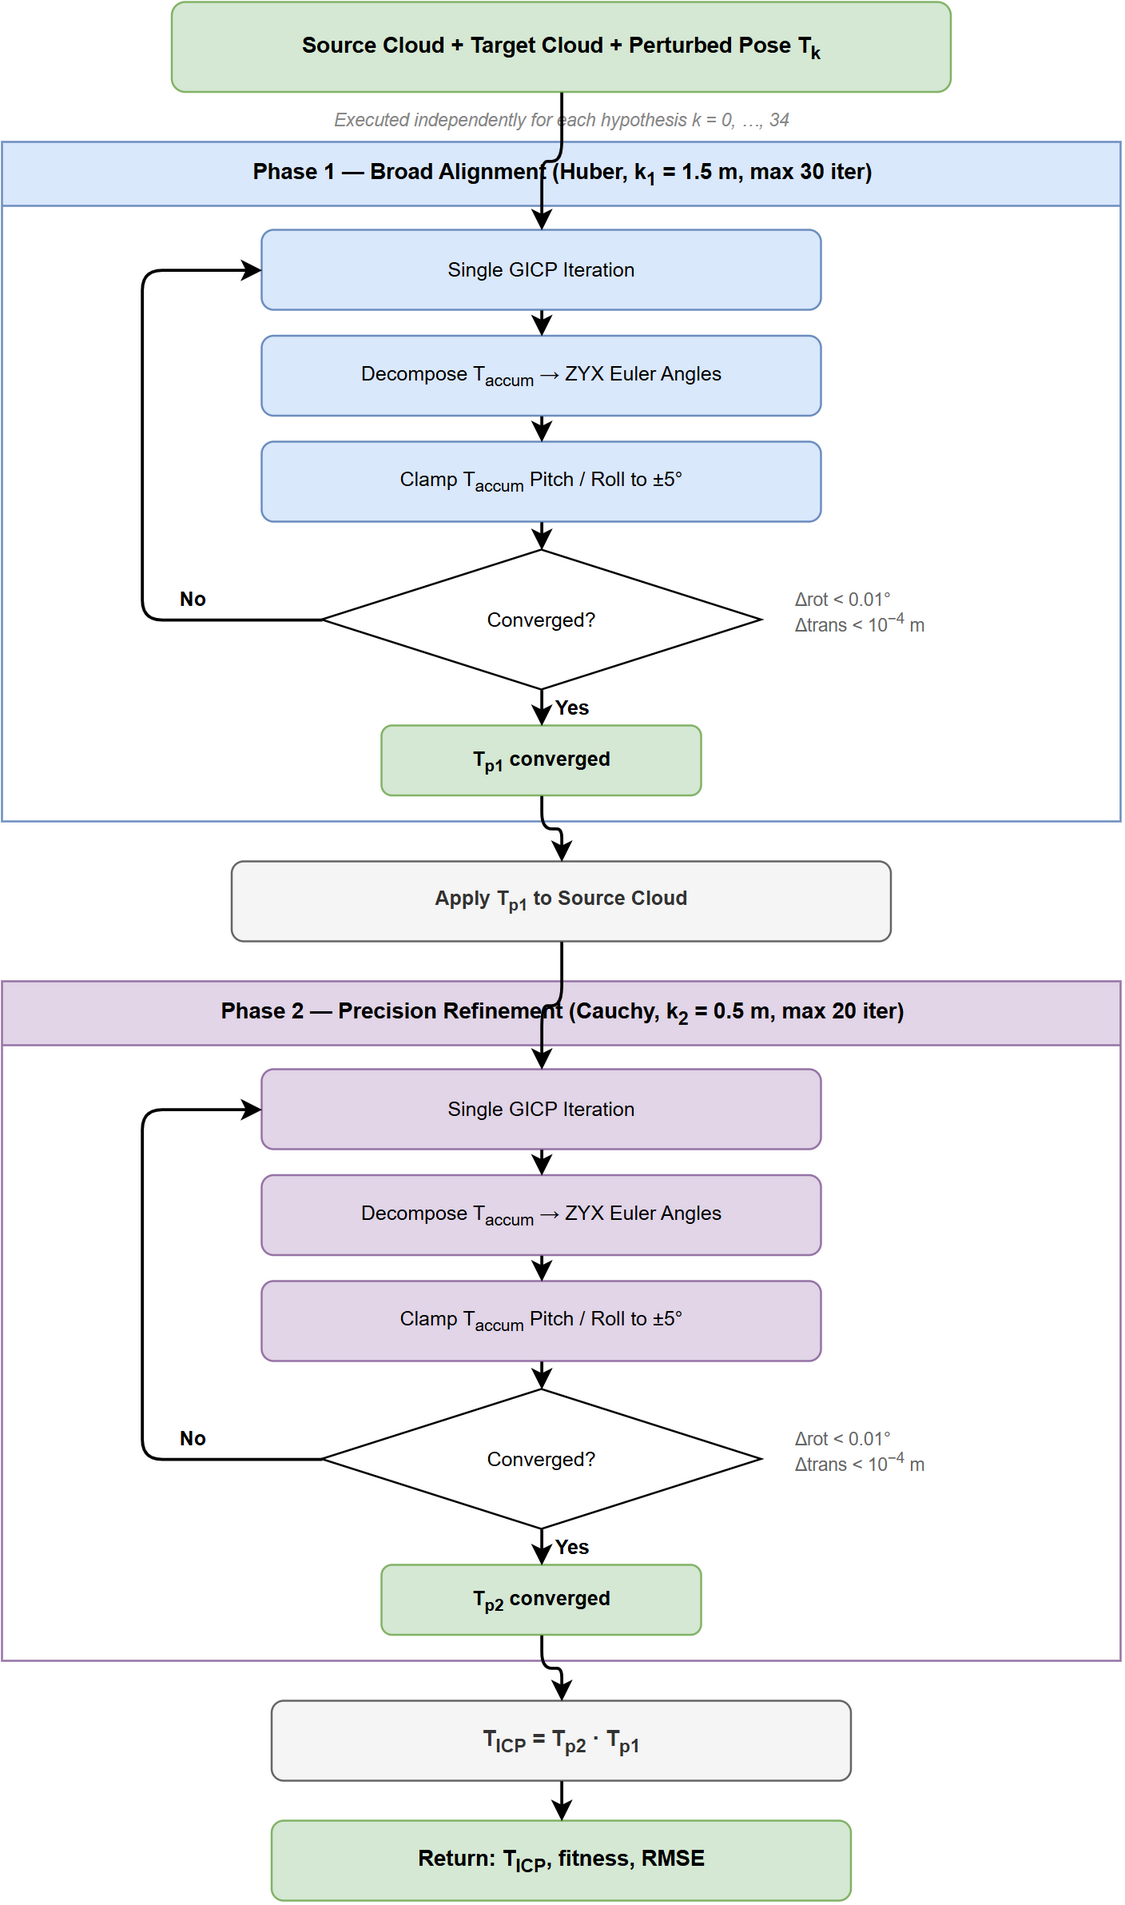
\includegraphics[width=0.75\linewidth]{4-precise-alignment/4-methodology/figures/pa-graduated-icp}
  \caption{Graduated GICP registration loop for a single perturbation hypothesis.
           Phase~1 uses a Huber loss ($k_1 = 1.5$\,m) for broad alignment;
           Phase~2 switches to a Cauchy loss ($k_2 = 0.5$\,m) for precision
           refinement. Both phases apply a rotation constraint
           that clamps the total accumulated pitch and roll correction to $\pm 10^{\circ}$.
           The final transformation is composed as
           $T_{\text{ICP}} = T_{\text{p2}} \cdot T_{\text{p1}}$.}
  \label{fig:pa-graduated-icp}
\end{figure}

\paragraph{Phase 1: Huber loss (broad alignment).}
The first phase uses a Huber robust loss function:
%
\begin{equation}
    \rho_H(r) =
    \begin{cases}
        \tfrac{1}{2} r^2                       & \text{if } |r| \leq k_1, \\
        k_1 \!\left(|r| - \tfrac{1}{2} k_1\right) & \text{otherwise,}
    \end{cases}
    \label{eq:huber-loss}
\end{equation}
%
where $r$ is the residual distance for a correspondence and $k_1 = 1.5$\,m is the scale parameter. Below $k_1$ the Huber loss is purely quadratic; above $k_1$ it grows linearly rather than being truncated entirely. The large value of $k_1$ means that the transition to linear growth occurs late, so the majority of correspondences, even those with substantial residuals early in registration, contribute a non-zero gradient and keep the optimisation from stalling. Phase~1 runs for a maximum of 30 iterations per hypothesis.

\paragraph{Phase 2: Cauchy loss (precision refinement).}
After Phase~1 brings the clouds into approximate alignment, the second phase switches to a Cauchy robust loss:
%
\begin{equation}
    \rho_C(r) = \frac{k_2^2}{2} \ln\!\left(1 + \left(\frac{r}{k_2}\right)^2\right),
    \label{eq:cauchy-loss}
\end{equation}
%
where $k_2 = 0.5$\,m. The Cauchy loss grows logarithmically for large residuals, so correspondences whose residuals exceed $k_2$ by even a modest factor are strongly down-weighted. With $k_2 = 0.5$, a residual of $0.75$\,m (i.e.\ $1.5\,k_2$) is already in the aggressive suppression regime, making Phase~2 sensitive only to the tightest inlier set. The Phase~1 converged transformation $T_{\text{p1}}$ is applied to the source cloud in place before Phase~2 begins, so that Phase~2 refines from the Phase~1 result. Phase~2 runs for a maximum of 20 iterations per hypothesis. The final combined transformation is:
%
\begin{equation}
    T_{\text{ICP}} = T_{\text{p2}} \cdot T_{\text{p1}},
    \label{eq:icp-combined}
\end{equation}
%
where $T_{\text{p2}}$ is the refinement returned by Phase~2.

\paragraph{Rotation constraint.}
Open3D's \texttt{registration\_generalized\_icp} provides no built-in mechanism for constraining the per-iteration correction. A custom iterative loop therefore replaces the library's internal iteration for both phases: at each step, a single GICP iteration is executed and the accumulated correction transform $T_{\text{accum}}$ (the total ICP-introduced change relative to the current phase's starting pose) is decomposed into ZYX Euler angles. The pitch and roll components of $T_{\text{accum}}$ are clamped to $\pm 10^{\circ}$; yaw and all three translation components remain unconstrained. Because the clamping is applied to $T_{\text{accum}}$ rather than to the absolute pose, it constrains only the correction introduced by ICP and preserves any pitch or roll present in the initial estimate. This is appropriate because the robot operates on approximately level terrain, so large pitch or roll corrections are more likely to be registration artefacts than genuine pose refinements.

Convergence in the constrained loop is declared when the incremental rotation between successive steps falls below $0.01^{\circ}$ and the incremental translation falls below $10^{-4}$\,m, or when the maximum iteration count for that phase is reached. Phase~1 clamps $T_{\text{accum}}$ relative to the initial perturbed pose; Phase~2 clamps $T_{\text{accum}}$ relative to the Phase~1 converged pose.

The parameters for the GICP registration stage are summarised in \cref{tab:pa-icp-params}.

\begin{table}[htbp]
  \centering
  \caption{GICP registration parameters.}
  \label{tab:pa-icp-params}
  \begin{tabularx}{\textwidth}{@{} >{\raggedright}p{0.27\textwidth} >{\raggedright}p{0.20\textwidth} >{\raggedright\arraybackslash}X @{}}
    \toprule
    \textbf{Parameter} & \textbf{Value} & \textbf{Description} \\
    \midrule
    Perturbation hypotheses         & 35                  & Total candidate poses: 1 nominal (Orig) + 34 perturbations (Groups~A, B, C, and~E; \cref{tab:pa-perturbation-groups}) \\
    Translation perturbation ($\delta_t$) & $0.10$\,m & Full magnitude used by Groups~B and~C; Group~A uses $\delta_t / 2 = 0.05$\,m \\
    Rotation perturbation ($\delta_r$)    & $10^{\circ}$ & Full magnitude used by Group~C (yaw component); Group~E uses both $\delta_r / 2 = 5^{\circ}$ and $\delta_r$ \\
    Voxel grid size ($v$)           & 0.0075\,m           & Downsampling resolution applied to source and target clouds \\
    GICP backend                    & Open3D              & \texttt{registration\_generalized\_icp}; generalised ICP implementation from Open3D~\cite{zhouOpen3DModernLibrary2018} \\
    Phase~1 loss (LiDAR)            & Huber, $k_1 = 1.5$\,m & Broad alignment phase; soft outlier rejection (\cref{eq:huber-loss}) \\
    Phase~1 max iterations          & 30                  & Per hypothesis \\
    Phase~2 loss (LiDAR)            & Cauchy, $k_2 = 0.5$\,m & Precision refinement phase; aggressive outlier rejection (\cref{eq:cauchy-loss}) \\
    Phase~2 max iterations          & 20                  & Per hypothesis \\
    Max correspondence distance     & 0.15\,m             & Maximum point-pair distance for correspondence acceptance \\
    Rotation constraint (LiDAR)     & $\pm 10^{\circ}$ pitch/roll & Clamp on total accumulated ICP correction; yaw unconstrained \\
    Constrained convergence: rotation    & $0.01^{\circ}$ & Inter-step rotation change threshold \\
    Constrained convergence: translation & $10^{-4}$\,m   & Inter-step translation change threshold \\
    Fitness threshold               & 0.8                 & Minimum fitness score for hypothesis acceptance \\
    \bottomrule
  \end{tabularx}
\end{table}

% ---------------------------------------------------------------
\subsection{Coordinate Frames and Pose Correction}
\label{subsec:pa-pose-correction}
% ---------------------------------------------------------------

The ICP registration stage returns a rigid transformation expressed in the sensor frame (that is, the frame of the camera or LiDAR sensor from which the source cloud was acquired). Before this result can be applied to the robot's localisation, it must be expressed in the base-link frame that serves as the canonical reference for all downstream planning and control components. It must also be introduced into the ROS~2 transform tree~\cite{macenskiRobotOperatingSystem2022} without disturbing the SLAM system's own transform publications.

\subsubsection*{Coordinate Frame Hierarchy}

The coordinate frame hierarchy used throughout this system is:
\[
  \texttt{local\_enu} \to \texttt{map} \to \texttt{odom} \to \texttt{base\_link} \to \texttt{sensor\_frame},
\]
where \texttt{local\_enu} is the ENU-anchored global frame, \texttt{map} and \texttt{odom} are the frames published by the SLAM system, \texttt{base\_link} is the robot body frame, and \texttt{sensor\_frame} is the frame of whichever sensor produced the source cloud. The static transforms between \texttt{base\_link} and the sensor frames are fixed by the mechanical configuration of the platform and are loaded at launch from the robot description.

\subsubsection*{TF Correction Mechanism}

A custom TF correction mechanism developed for this work inserts a correction frame into the transform tree without modifying any of the transforms published by the SLAM system. The ICP result provides the correction in the sensor frame, $T_{\mathrm{correction, sensor}}$. To express this correction at the level of the base link, the following composition is applied:
%
\begin{equation}
    T_{\mathrm{correction, base}} =
        T_{\mathrm{base} \to \mathrm{sensor}}^{-1}
        \cdot T_{\mathrm{correction, sensor}}
        \cdot T_{\mathrm{base} \to \mathrm{sensor}},
    \label{eq:tf-correction}
\end{equation}
%
where $T_{\mathrm{base} \to \mathrm{sensor}}$ is the fixed extrinsic transform from the base link to the sensor frame. The resulting base-frame correction is then inserted into the appropriate location in the transform chain and published as a static transform, as illustrated in \cref{fig:pa-tf-correction}.

\begin{figure}[htbp]
  \centering
  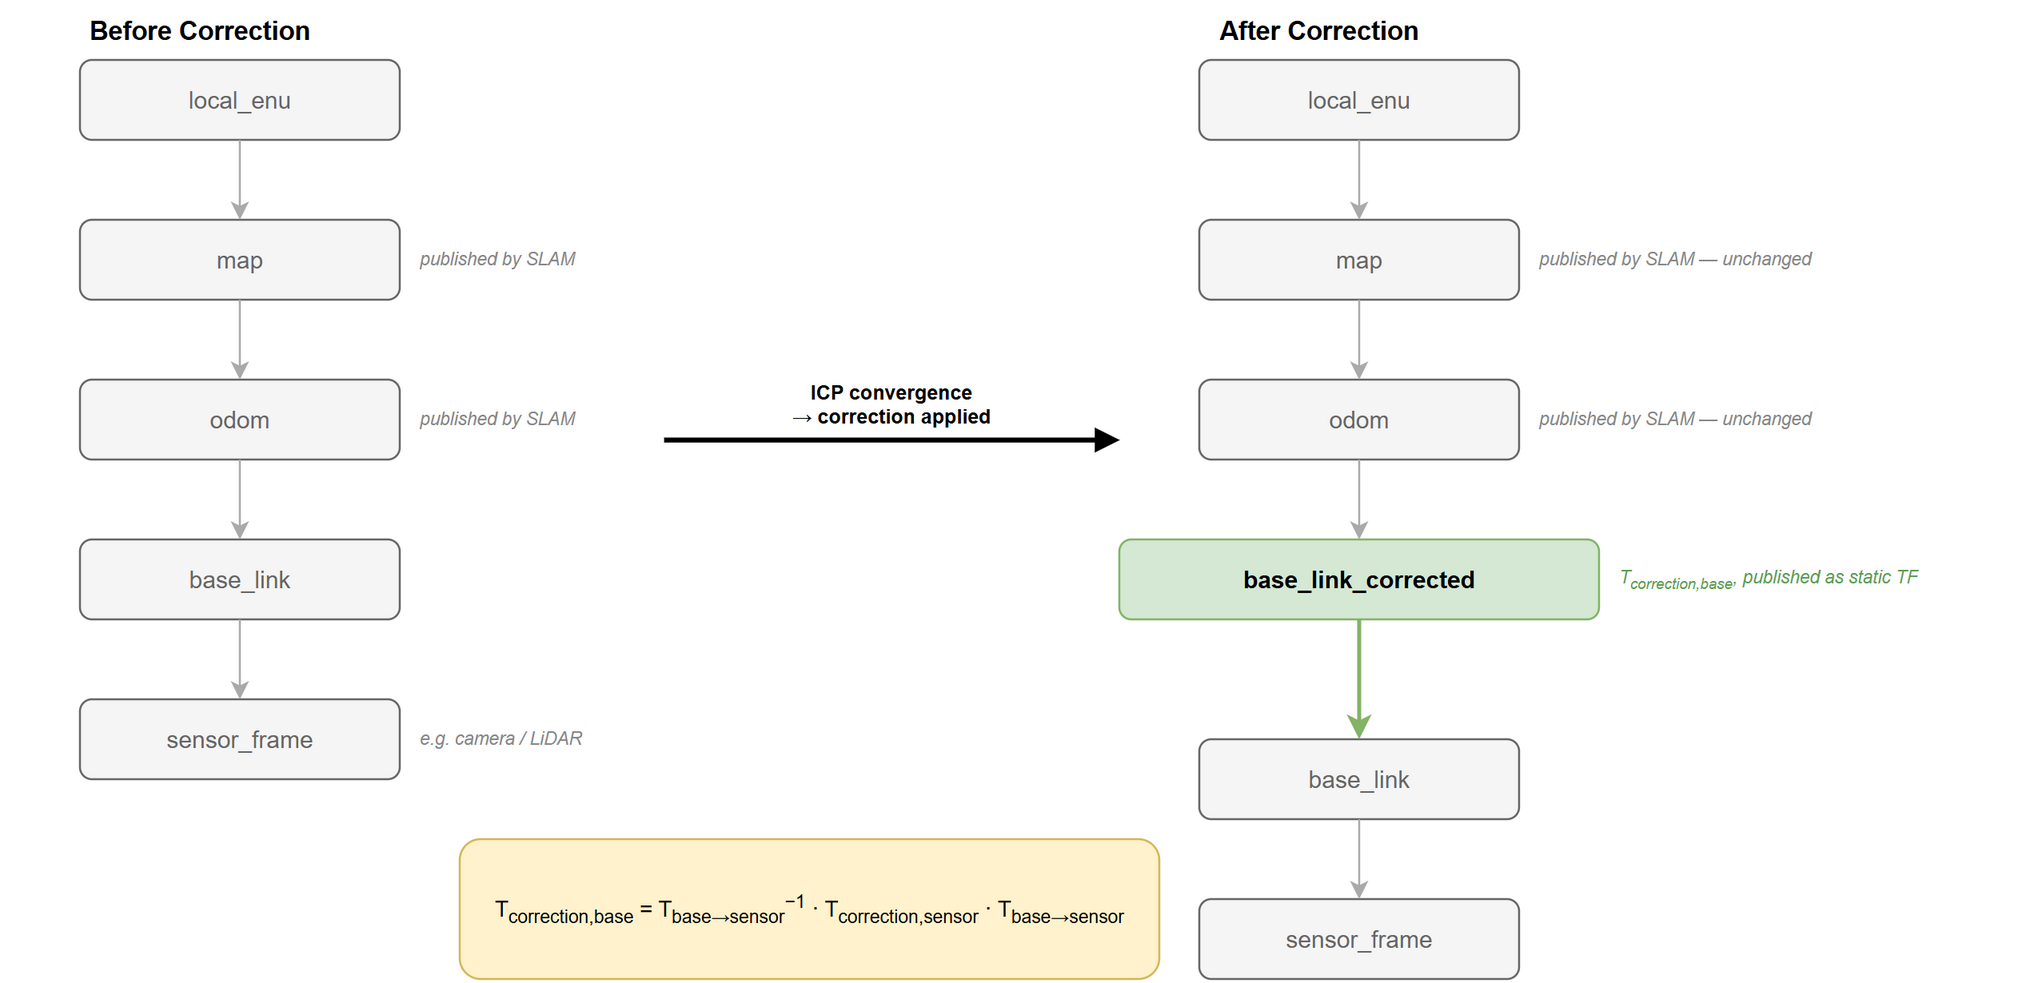
\includegraphics[width=\linewidth]{4-precise-alignment/4-methodology/figures/pa-tf-correction}
  \caption{ROS~2 TF transform tree before (left) and after (right) insertion of the pose
           correction frame. The correction is introduced between the SLAM-published
           \texttt{odom} frame and downstream planning frames without modifying the SLAM
           system's own publications. $T_{\mathrm{correction,base}}$ is derived from the
           ICP result via the extrinsic $T_{\mathrm{base} \to \mathrm{sensor}}$
           (\cref{eq:tf-correction}).}
  \label{fig:pa-tf-correction}
\end{figure}

Because the correction is published as a static transform, it does not require a continuous update loop and is non-disruptive to the SLAM publishers. The correction mechanism supports both automatic triggering (applied immediately upon successful ICP convergence) and manual triggering, in which the operator confirms before the correction is broadcast to the transform tree. The appropriate mode is selected at launch via a configuration parameter.

% ---------------------------------------------------------------
\subsection{Pipeline Execution Model}
\label{subsec:pa-execution-model}
% ---------------------------------------------------------------

Each precise alignment request is encapsulated as an ordered sequence of command objects following the Command design pattern. Each processing stage (depth estimation, point cloud preprocessing, target cloud extraction, ICP registration, and pose correction) is implemented as an \texttt{AsyncCommand} with a well-defined input contract and output contract. Commands are submitted to an asynchronous task queue, which executes them sequentially within a dedicated worker thread pool. This design decouples the processing pipeline from the ROS~2 executor event loop: computationally intensive operations such as FoundationStereo inference and Open3D ICP run in non-blocking threads, avoiding latency spikes in the ROS~2 message-handling callbacks. The execution architecture is illustrated in \cref{fig:pa-execution-model}.

\begin{figure}[htbp]
  \centering
  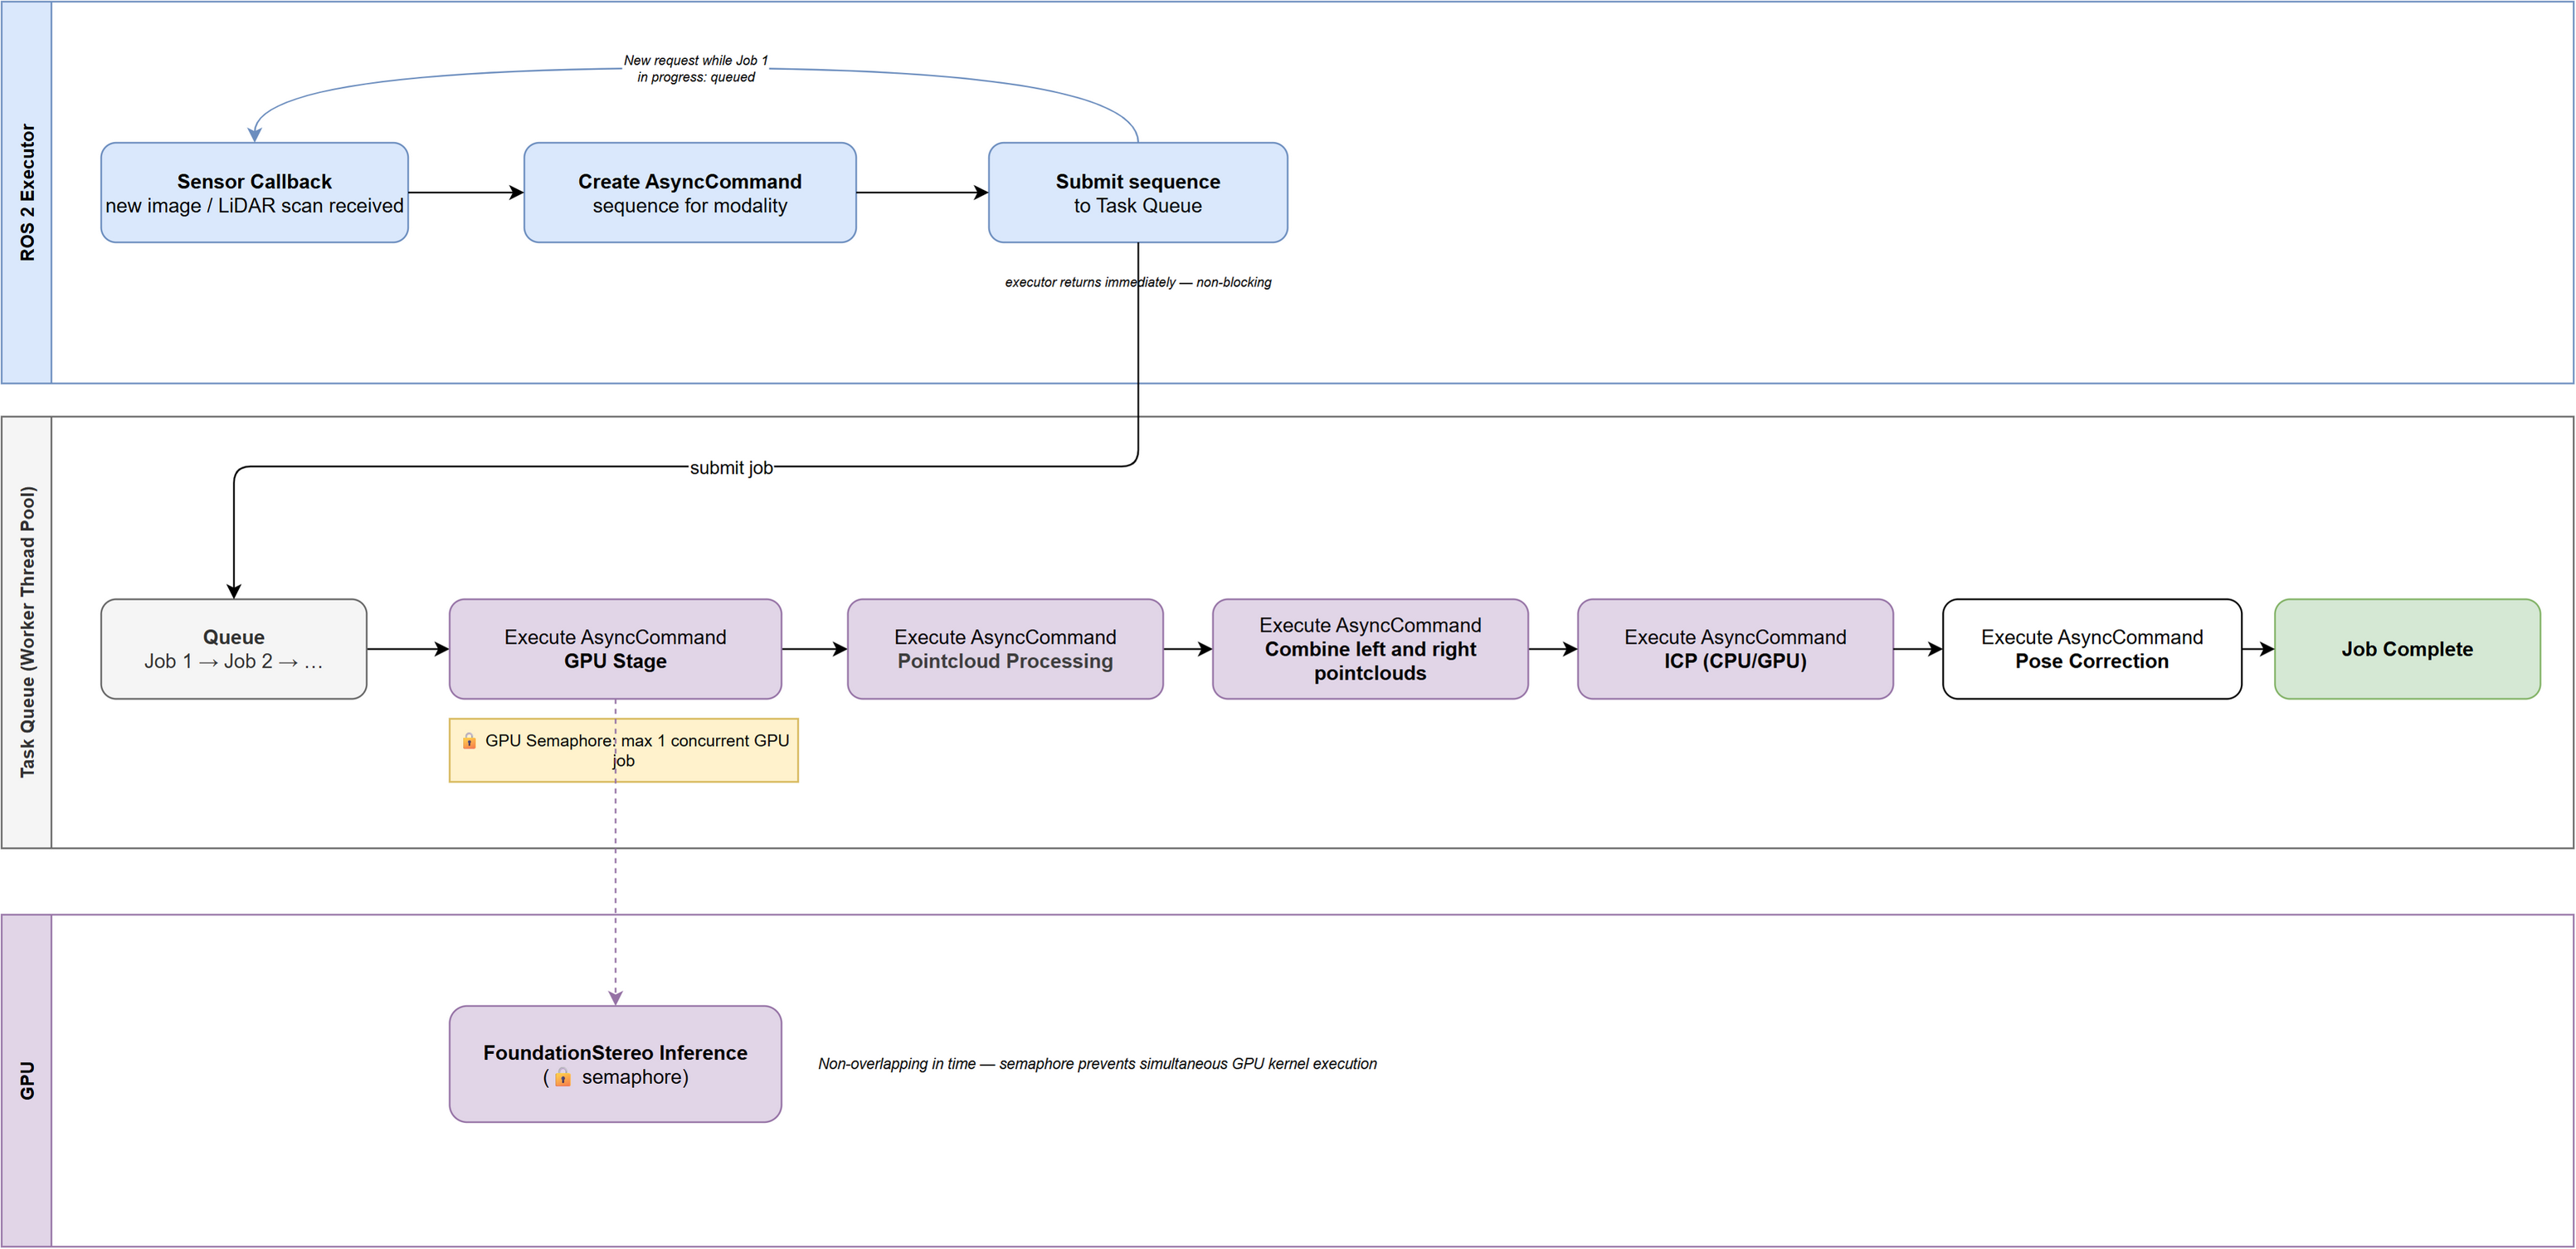
\includegraphics[width=\linewidth]{4-precise-alignment/4-methodology/figures/pa-execution-model}
  \caption{Pipeline execution model for the stereo modality. The LiDAR pipeline
           follows the same structure with modality-specific command steps.}
  \label{fig:pa-execution-model}
\end{figure}

The GPU-resident FoundationStereo inference stage is governed by a semaphore-based concurrency guard that prevents simultaneous kernel execution from exceeding available GPU memory. Target cloud extraction from the 3DGS model reads Gaussian mean positions on the CPU and is not subject to this guard. When a new alignment request arrives while a prior job is still processing, it enters the pipeline as soon as the first stage becomes available; the stages are pipelined such that a subsequent job may begin executing a stage once the preceding job has advanced beyond it, allowing multiple jobs to be processed concurrently at different stages. This execution model supports both the stereo and LiDAR pipelines without modification, as the modality-specific processing difference is captured entirely within the command sequence submitted for each observation type.

The preceding subsections have described the complete precise alignment pipeline: sensor preprocessing for both stereo and LiDAR observations, target point cloud extraction from the 3DGS model, GICP registration with neighbourhood perturbation, and pose correction. The following subsection describes the experimental setup designed to evaluate the LiDAR pipeline under controlled conditions. The results of these experiments are presented in \cref{sec:precise-alignment-results}.

% ===============================================================
\subsection{Experimental Setup}
\label{subsec:pa-experimental-setup}
% ===============================================================
% TODO: document the computational resources used for evaluation: (1) robot onboard compute (CPU, GPU, RAM) and (2) local machine specs (CPU, GPU, RAM) used to run evals offline.

This section describes the experimental setup used to evaluate the precise-alignment pipeline. LiDAR and stereo data were recorded simultaneously during each trial; both sensing modalities are therefore evaluated against the same set of trial conditions. Six aspects of the evaluation are described: the test environment, the vine specimen and reference model, the trial design, the construction of initial poses, the evaluation protocol, and the metrics used to validate alignment quality.

% ---------------------------------------------------------------
\subsubsection{Test Environment}
\label{subsubsec:pa-test-environment}
% ---------------------------------------------------------------

Trials were conducted in an indoor laboratory environment. This study is scoped to dormant-season vineyard conditions, in which vines present a leafless, woody skeletal structure. At the time of evaluation, vines in the field retained their autumn foliage, rendering outdoor vineyard environments unsuitable for testing the pipeline under its intended operating conditions. Two dead vine specimens were therefore sourced from a vineyard and mounted side by side on an aluminium support rig fitted with tensioned guide wires, replicating the structural arrangement of a vineyard bay. Although no longer living, the specimens retain their woody trunk and cane structure, which is characteristic of dormant vines and is considered representative of the target scenario.

Outdoor validation was also precluded for a practical reason. The 3DGS reference model was reconstructed from outdoor SfM photogrammetry of the specimen at its original collection site. Subsequent construction at that site has rendered it inaccessible, precluding live-registration trials under the original georeferenced coordinate frame. The specimens were accordingly relocated to the indoor laboratory, where they were mounted on the support rig and the 3DGS model's coordinate system was manually aligned to the laboratory frame. The indoor laboratory therefore served as a controlled proxy environment; outdoor validation under field conditions remains future work.

Several limitations of the indoor evaluation should be noted. First, the dead specimens may exhibit different surface reflectance characteristics compared with living dormant vines; LiDAR return intensity and noise profiles may therefore not be fully representative of field conditions, though the woody geometric structure is preserved. Second, the aluminium support rig introduces structural elements like posts and tensioned wires that are not identical to those found in a real vineyard bay; however, since vineyard bays similarly feature vertical timber posts and tensioned guide wires, the overall structural character of the scene is considered broadly representative. Third, any residual error in the manual alignment of the 3DGS model to the laboratory coordinate system is indistinguishable from pipeline registration error in the reported metrics. The physical arrangement of the laboratory, including the vine specimen, robot platform, and sensor positions, is illustrated in \cref{fig:pa-lab-setup}.

\begin{figure}[htbp]
  \centering
  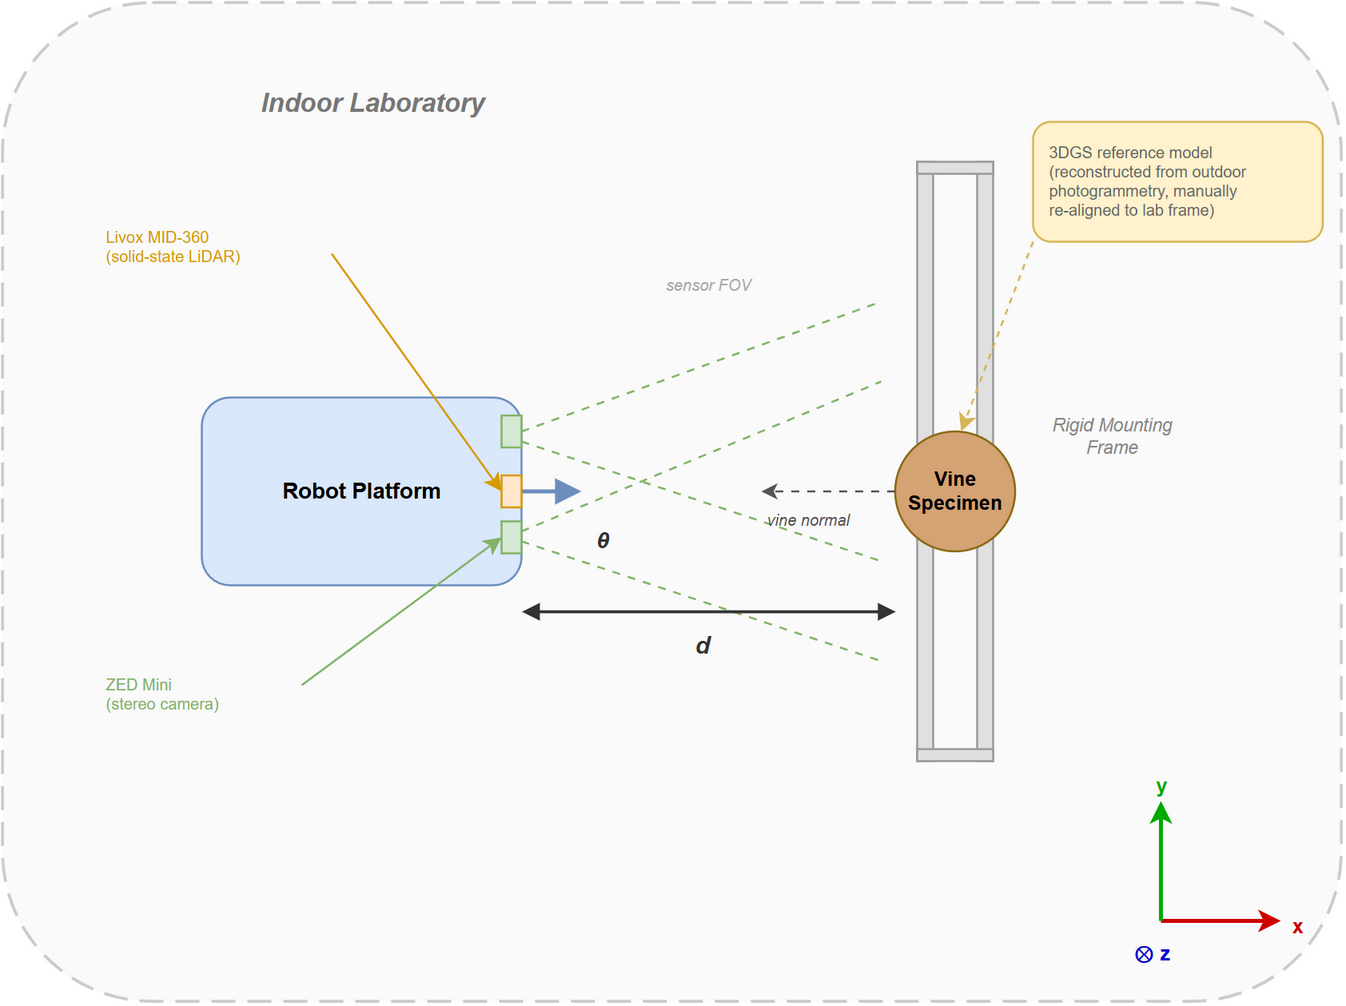
\includegraphics[width=0.85\linewidth]{4-precise-alignment/4-methodology/figures/pa-lab-setup}
  \caption{Physical layout of the indoor laboratory test environment (top-down view).
           The vine specimen is mounted on a rigid frame at a fixed position; the
           robot platform is positioned facing the vine with the Livox LiDAR and
           ZED~Mini stereo camera on its vine-facing side. The distance~$d$ and
           approach angle~$\theta$ define the operating condition for each trial.
           The 3DGS reference model, reconstructed from outdoor photogrammetry,
           was manually re-aligned to the laboratory coordinate frame.}
  \label{fig:pa-lab-setup}
\end{figure}

% ---------------------------------------------------------------
\subsubsection{Vine Specimen and Reference Model}
\label{subsubsec:pa-vine-specimen}
% ---------------------------------------------------------------

A dormant vine specimens were mounted on a rigid physical frame to replicate the vertical trunk structure encountered in a vineyard row. Mounting the specimen on a fixed support ensured that the vine remained stationary throughout all trials, eliminating inter-trial positional drift as a confounding factor.

The 3DGS reference model used for registration was reconstructed from outdoor SfM photogrammetry of the same vine specimen, following the procedure described in \cref{subsec:system-context}. The model is georeferenced in the ENU coordinate frame. For the indoor trials, the model's coordinate system was manually aligned to the laboratory environment to establish a consistent spatial reference between the physical specimen and the model. This alignment provided the common frame of reference required by the registration pipeline.

% ---------------------------------------------------------------
\subsubsection{Trial Design}
\label{subsubsec:pa-trial-design}
% ---------------------------------------------------------------

Trials were organised as a structured evaluation across nine operating conditions defined by two factors: the distance from the sensor to the vine trunk ($d$) and the lateral approach angle ($\theta$) relative to the vine normal. Three levels were selected for each factor: $d \in \{40, 60, 80\}$\,cm and $\theta \in \{-15^{\circ}, 0^{\circ}, {+}15^{\circ}\}$, yielding nine unique conditions that sample the operational envelope at representative points. One additional replicate at the centre condition ($d = 60$\,cm, $\theta = 0^{\circ}$) was included as a repeatability check, resulting in ten trials in total. Because only a single observation is available per non-centre condition, the evaluation is exploratory in nature and does not support formal statistical inference; results characterise pipeline behaviour across the sampled operating conditions rather than quantifying main effects or interactions.

The full trial matrix is summarised in \cref{tab:pa-trial-matrix}; the corresponding spatial layout is shown in \cref{fig:pa-trial-layout}.

\begin{table}[htbp]
  \centering
  \caption{Experimental trial matrix. Each row defines one trial with its distance and angle factor levels. Trial~D60A0r is a replicate of the centre condition (60\,cm, 0$^{\circ}$).}
  \label{tab:pa-trial-matrix}
  \begin{tabularx}{\textwidth}{l c c}
    \toprule
    \textbf{Trial ID} & \textbf{Distance (cm)} & \textbf{Angle ($^{\circ}$)} \\
    \midrule
    D40A-15 & 40 & $-15$ \\
    D40A0   & 40 &    $0$ \\
    D40A15  & 40 & ${+}15$ \\
    D60A-15 & 60 & $-15$ \\
    D60A0   & 60 &    $0$ \\
    D60A15  & 60 & ${+}15$ \\
    D80A-15 & 80 & $-15$ \\
    D80A0   & 80 &    $0$ \\
    D80A15  & 80 & ${+}15$ \\
    D60A0r  & 60 &    $0$ \\
    \bottomrule
  \end{tabularx}
\end{table}

An additional trial at 110\,cm ($d = 110$, $\theta = 0^{\circ}$) was collected during the experimental session but is excluded from analysis. This distance exceeds the stereo pipeline's near-field depth clipping threshold ($z_\text{far} = 1.0$\,m), rendering the condition invalid by design for the stereo modality. To maintain a consistent condition set across both modalities, the D110A0 trial is omitted from all reported results.

\begin{figure}[htbp]
  \centering
  \includegraphics[width=0.7\linewidth]{4-precise-alignment/4-methodology/figures/pa-trial-layout}
  \caption{Spatial layout of the experimental trial conditions (top-down view).
           Nine unique operating conditions are defined by crossing three
           sensor-to-vine distances ($d \in \{40, 60, 80\}$\,cm) with three
           lateral approach angles ($\theta \in \{-15^{\circ}, 0^{\circ},
           {+}15^{\circ}\}$). Trial~D60A0r is a replicate of the centre
           condition. Each blue marker indicates the robot sensor position
           relative to the vine trunk for the corresponding trial.}
  \label{fig:pa-trial-layout}
\end{figure}

% ---------------------------------------------------------------
\subsubsection{Initial Pose Construction}
\label{subsubsec:pa-initial-pose}
% ---------------------------------------------------------------

For each trial, the initial pose was constructed from a manual measurement of the robot's position and orientation relative to the vine specimen. The measurement was encoded as a $4 \times 4$ homogeneous transformation matrix in $SE(3)$ and provided to the localisation pipeline as a substitute for the SLAM-derived initial pose that would be available in a deployed system. This approach allows the registration stage to be evaluated in isolation from the SLAM system, with full control over the initial pose quality.

The distance component was measured with a steel tape measure as the orthogonal distance from a fixed reference point on the vine mounting frame to the LiDAR sensor on the robot. The approach angle was determined by triangulation: from the same reference point, the orthogonal distance to the robot was measured, and a second perpendicular was projected from the robot base back to the vine frame. The distance along the frame between the original reference point and this second intersection point, together with the two perpendicular measurements, defined a triangle from which the approach angle was computed trigonometrically. The measurement geometry is illustrated in \cref{fig:pa-pose-measurement}.

\begin{figure}[htbp]
  \centering
  \includegraphics[width=0.65\linewidth]{4-precise-alignment/4-methodology/figures/pa-pose-measurement}
  \caption{Initial pose measurement geometry (top-down view). The approach
           angle~$\theta$ is determined by triangulation from the vine reference
           point~$P$ on the mounting frame. A perpendicular from the robot sensor
           position~$R$ back to the frame intersects at~$Q$; the lateral offset~$PQ$
           along the frame and the perpendicular distance~$QR$ define a right
           triangle from which $\theta = \arctan(PQ / QR)$ is computed.}
  \label{fig:pa-pose-measurement}
\end{figure}

The manual measurement procedure introduces a positioning uncertainty on the order of $\pm 2$--$3$\,cm in translation and $\pm 2$--$3^{\circ}$ in orientation. The translational uncertainty reflects the combined precision of the tape measure ($\pm 1$\,mm) and the difficulty of consistently identifying the reference point on the frame and the sensor centre on the robot; the angular uncertainty reflects the propagation of these linear measurement errors through the trigonometric angle computation. This uncertainty is substantially smaller than the absolute trajectory error (ATE) observed for the GLIM SLAM system~\cite{koideGLIM3DRangeInertial2024} with GNSS fusion in the outdoor evaluation presented in \cref{sec:slam-results}, where the ATE ranges from 0.07 to 0.17\,m. The manual measurement therefore represents a \emph{more favourable} initial condition than would be encountered in deployment. As a consequence, any alignment failures observed under these laboratory conditions indicate a fundamental limitation of the registration pipeline itself, rather than an artefact of poor initial pose quality.

% ---------------------------------------------------------------
\subsubsection{Evaluation Protocol}
\label{subsubsec:pa-eval-protocol}
% ---------------------------------------------------------------

The per-trial evaluation workflow is illustrated in \cref{fig:pa-eval-flowchart}. For each trial, the pipeline generated 35 perturbation hypotheses distributed around the initial pose, following the perturbation protocol described in \cref{subsec:pa-icp-registration}. Each hypothesis was registered independently using GICP against the target point cloud extracted from the 3DGS model; convergence criteria for the ICP solver are as specified in \cref{tab:pa-icp-params}.

\begin{figure}[htbp]
  \centering
  \includegraphics[width=0.85\linewidth]{4-precise-alignment/4-methodology/figures/pa-eval-flowchart}
  \caption{Per-trial evaluation protocol. The initial pose is perturbed to
           generate 35 candidate hypotheses (Orig and Groups~A, B, C,~and~E), each registered
           independently via GICP. Per-hypothesis fitness and RMSE are recorded;
           hypotheses with fitness below~0.8 are rejected, and the best remaining
           result is selected. Three complementary validation strategies (perturbation convergence consistency, inter-trial consistency, and
           visual overlay) are applied to the serialised results.}
  \label{fig:pa-eval-flowchart}
\end{figure}

The following quantities were recorded for each hypothesis:
%
\begin{itemize}
  \item \textbf{Fitness score}: the ratio of inlier correspondences to the total number of source points;
  \item \textbf{Inlier RMSE}: the root-mean-square error of the accepted inlier correspondences;
  \item \textbf{Estimated transformation}: the $4 \times 4$ matrix in $SE(3)$ representing the registration result;
  \item \textbf{Euler angle decomposition}: a decomposition of the estimated rotation into roll, pitch, and yaw angles, retained for interpretability.
\end{itemize}
%
All per-trial results were serialised to JSON for subsequent analysis. Wall-clock timing was additionally recorded for each trial to assess computational feasibility. The following intervals were measured: total pipeline latency from trigger to corrected pose publication, preprocessing time from raw sensor data to filtered source cloud, and GICP registration time across all 35 hypotheses including hypothesis selection. These timings are reported as mean $\pm$ standard deviation across trials.

% ---------------------------------------------------------------
\subsubsection{Evaluation Metrics and Validation}
\label{subsubsec:pa-eval-metrics}
% ---------------------------------------------------------------

Two primary metrics are used to assess registration quality. The fitness score measures the fraction of source points for which a valid correspondence exists within the maximum correspondence distance threshold; a higher fitness score indicates that a greater proportion of the observed structure is geometrically consistent with the reference model. The inlier RMSE measures the geometric residual of accepted correspondences; lower values indicate tighter point-to-point alignment.

Results are additionally analysed per perturbation group (Orig and Groups~A, B, C, and~E, as defined in \cref{subsec:pa-icp-registration}) to assess whether certain perturbation directions are systematically more or less conducive to convergence. This per-group breakdown reveals whether the pipeline exhibits sensitivity to specific classes of initial pose error.

Three complementary validation strategies are applied. First, \emph{perturbation convergence consistency} assesses whether multiple hypotheses within a single trial converge to similar final poses; large dispersion across hypotheses indicates sensitivity to initialisation rather than a stable registration basin. Second, \emph{inter-trial consistency} examines whether similar factor conditions, for example the same distance at different approach angles, produce comparable fitness and RMSE values, providing evidence that results are not artefacts of a single fortuitous initial pose. Third, \emph{visual overlay} provides qualitative validation by rendering the registered source cloud and target cloud in a common frame for visual inspection of alignment quality. Cross-modal validation, comparing LiDAR and stereo registration outcomes on matched trials, is deferred to the stereo experimental setup section.

Because only a single trial is conducted per non-centre condition, formal statistical tests (e.g.\ ANOVA or interaction-effect estimation) are not applicable. Results are instead presented as a condition-by-condition summary: for each trial, the number of hypotheses exceeding the fitness acceptance threshold, the median and interquartile range (IQR) of fitness and RMSE across accepted hypotheses, and the spread of the recovered transformation components. Cross-condition trends, for example whether fitness degrades with increasing distance or whether oblique angles produce higher RMSE variability, are discussed qualitatively. If the replicate pair (D60A0 and D60A0r) yields consistent results, this is noted as evidence of repeatability; discrepancies are discussed.

\paragraph{Limitations.}
No external six-degree-of-freedom ground truth was available for these trials. The fitness score and inlier RMSE are \emph{internal} registration metrics: they measure how well the source cloud matches the target cloud, but do not directly measure whether the recovered pose corresponds to the robot's true physical pose. A high fitness score is necessary but not sufficient for correct alignment, since ICP can converge to a local minimum that achieves good geometric consistency without recovering the true transformation. Visual overlay provides a qualitative cross-check against gross misalignment, and the consistency of results across the 35 perturbation hypotheses provides evidence that the registration basin is stable. However, the results should be interpreted as evidence of geometric consistency between the sensor observation and the 3DGS reference model, rather than as a direct measurement of absolute pose accuracy. Outdoor validation with surveyed reference poses or a motion capture system would be required to quantify absolute accuracy and remains future work.

% ===========================================================================
\section{Results}
\label{sec:precise-alignment-results}
% ===========================================================================

This section reports quantitative registration results for both the LiDAR and stereo precise-alignment pipelines across nine experimental conditions conducted in the indoor laboratory environment described in \cref{subsubsec:pa-test-environment}. The nine conditions span a $3 \times 3$ factorial design of sensor-to-vine distance ($d \in \{40, 60, 80\}$\,cm) and approach angle ($\alpha \in \{-15^{\circ}, 0^{\circ}, +15^{\circ}\}$). Each LiDAR trial generates 35 perturbation hypotheses, yielding 315 hypothesis-level results in total; the stereo pipeline executes a single ICP run per trial. \Cref{tab:pa-results-condition-map} defines the mapping between experimental conditions and data identifiers.

% ---------------------------------------------------------------------------
\subsection{Trial Conditions and Mapping}
\label{subsec:pa-results-condition-map}
% ---------------------------------------------------------------------------

\begin{table}[htbp]
  \centering
  \caption{Experimental condition mapping. Each condition specifies the sensor-to-vine distance $d$ (cm) and approach angle $\alpha$ (degrees).}
  \label{tab:pa-results-condition-map}
  \begin{tabular}{@{} l r r @{}}
    \toprule
    \textbf{Condition} & \boldmath$d$ \textbf{(cm)} & \boldmath$\alpha$ \textbf{(°)} \\
    \midrule
    D40A$-$15 &  40 & $-$15 \\
    D40A0     &  40 &     0 \\
    D40A$+$15 &  40 & $+$15 \\
    D60A$-$15 &  60 & $-$15 \\
    D60A0     &  60 &     0 \\
    D60A$+$15 &  60 & $+$15 \\
    D80A$-$15 &  80 & $-$15 \\
    D80A0     &  80 &     0 \\
    D80A$+$15 &  80 & $+$15 \\
    \bottomrule
  \end{tabular}
\end{table}

% ---------------------------------------------------------------------------
\subsection{LiDAR Registration Performance}
\label{subsec:pa-results-lidar-summary}
% ---------------------------------------------------------------------------

\Cref{tab:pa-results-lidar-per-condition} summarises the LiDAR registration outcome for each condition. For each trial the table reports the number of points in the preprocessed source cloud, the number and proportion of the 35 hypotheses that exceeded the fitness acceptance threshold ($F \geq 0.8$), and the median and interquartile range (IQR) of the fitness score and inlier RMSE across accepted hypotheses.

\begin{table}[htbp]
  \centering
  \small
  \setlength{\tabcolsep}{4pt}
  \caption{Per-condition LiDAR registration summary. Median and IQR statistics are computed over accepted hypotheses only ($F \geq 0.8$). All inlier RMSE values are in millimetres.}
  \label{tab:pa-results-lidar-per-condition}
  \begin{tabular}{@{} l r r r r r r r @{}}
    \toprule
    \textbf{Condition} &
    \textbf{Proc.\ pts} &
    \boldmath$n_\text{acc}$\textbf{/35} &
    \textbf{\%} &
    \boldmath$\tilde{F}$ &
    \textbf{IQR(}\boldmath$F$\textbf{)} &
    \boldmath$\tilde{\varepsilon}$ \textbf{(mm)} &
    \textbf{IQR(}\boldmath$\varepsilon$\textbf{) (mm)} \\
    \midrule
    D40A$-$15 &  97\,358 & 35/35 & 100 & 0.8939 & 0.0079 & 32.31 & 2.37 \\
    D40A0     & 112\,312 & 34/35 &  97 & 0.9107 & 0.0000 & 35.22 & 0.27 \\
    D40A$+$15 & 111\,880 & 35/35 & 100 & 0.9042 & 0.0000 & 34.85 & 0.59 \\
    D60A$-$15 & 116\,892 & 35/35 & 100 & 0.9205 & 0.0001 & 34.94 & 0.10 \\
    D60A0     & 108\,707 & 35/35 & 100 & 0.9174 & 0.0000 & 33.25 & 0.00 \\
    D60A$+$15 & 111\,880 & 35/35 & 100 & 0.9042 & 0.0000 & 34.84 & 0.58 \\
    D80A$-$15 & 116\,750 & 35/35 & 100 & 0.9141 & 0.0001 & 23.38 & 0.02 \\
    D80A0     & 121\,350 & 32/35 &  91 & 0.9277 & 0.0000 & 24.41 & 0.00 \\
    D80A$+$15 & 133\,017 & 35/35 & 100 & 0.9160 & 0.0000 & 23.77 & 0.00 \\
    \midrule
    \textbf{Aggregate} & --- & 311/315 & 98.7 & 0.9141 & 0.0133 & 33.25 & 10.47 \\
    \bottomrule
  \end{tabular}
\end{table}

All nine conditions achieved full or near-full hypothesis acceptance ($\geq 91\%$). Of the 315 hypotheses evaluated, 311 were accepted (98.7\%). The lowest per-condition acceptance rate was D80A0 at 91\% (32/35); the remaining eight conditions achieved 97--100\%.

% ---------------------------------------------------------------------------
\subsection{Per-Perturbation-Group Results}
\label{subsec:pa-results-perturbation-groups}
% ---------------------------------------------------------------------------

The 35 hypotheses generated per trial are organised into five perturbation groups. Statistics in \cref{tab:pa-results-groups} are aggregated across all nine conditions (315 hypotheses total); metrics are computed over accepted hypotheses only.

\begin{itemize}
  \item \emph{Orig} (1 per trial): the nominal, unperturbed initial pose.
  \item \emph{Group~A} (6 per trial): axis-aligned translation perturbations ($\pm x$, $\pm y$, $\pm z$).
  \item \emph{Group~B} (4 per trial): cardinal-direction translations (N, E, S, W).
  \item \emph{Group~C} (12 per trial): compound perturbations combining diagonal translations with yaw rotations.
  \item \emph{Group~E} (12 per trial): rotation-only perturbations sweeping yaw, pitch, and roll.
\end{itemize}

\begin{table}[htbp]
  \centering
  \small
  \setlength{\tabcolsep}{4pt}
  \caption{Per-perturbation-group registration results, aggregated across all nine conditions (315 hypotheses total). Statistics computed over accepted hypotheses only.}
  \label{tab:pa-results-groups}
  \begin{tabular}{@{} l r r r r r r @{}}
    \toprule
    \textbf{Group} &
    \boldmath$n_\text{acc}$\textbf{/}\boldmath$n_\text{hyp}$ &
    \textbf{\%} &
    \boldmath$\tilde{F}$ &
    \textbf{IQR(}\boldmath$F$\textbf{)} &
    \boldmath$\tilde{\varepsilon}$ \textbf{(mm)} &
    \textbf{IQR(}\boldmath$\varepsilon$\textbf{) (mm)} \\
    \midrule
    Orig   &   9/9   & 100 & 0.9142 & 0.0133 & 34.28 & 10.25 \\
    A      &  54/54  & 100 & 0.9141 & 0.0133 & 33.25 & 10.47 \\
    B      &  36/36  & 100 & 0.9141 & 0.0133 & 33.77 & 10.44 \\
    C      & 105/108 &  97 & 0.9107 & 0.0133 & 34.84 & 10.62 \\
    E      & 107/108 &  99 & 0.9141 & 0.0133 & 33.25 & 10.47 \\
    \midrule
    \textbf{All} & 311/315 & 99 & 0.9141 & 0.0133 & 33.25 & 10.47 \\
    \bottomrule
  \end{tabular}
\end{table}

Acceptance rates range from 97\% (Group~C) to 100\% (Orig, A, B). Median fitness and RMSE are consistent across all groups.

% ---------------------------------------------------------------------------
\subsection{LiDAR: Distance and Angle Effects}
\label{subsec:pa-results-lidar-distance-angle}
% ---------------------------------------------------------------------------

\Cref{tab:pa-results-lidar-by-distance,tab:pa-results-lidar-by-angle} present registration outcomes grouped by sensor-to-vine distance and approach angle, respectively.

\begin{table}[htbp]
  \centering
  \caption{LiDAR registration results grouped by sensor-to-vine distance. Best-hypothesis fitness and RMSE are reported (median across conditions within each distance group). All RMSE values in millimetres.}
  \label{tab:pa-results-lidar-by-distance}
  \begin{tabular}{@{} l r r r r r @{}}
    \toprule
    \textbf{Distance} &
    \textbf{Conditions} &
    \boldmath$n_\text{acc}$\textbf{/}\boldmath$n_\text{total}$ &
    \textbf{\%} &
    \textbf{Med.\ best} \boldmath$F$ &
    \textbf{Med.\ best} \boldmath$\varepsilon$ \textbf{(mm)} \\
    \midrule
    D40 (40\,cm)  & 3 & 104/105 &  99 & 0.9042 & 34.66 \\
    D60 (60\,cm)  & 3 & 105/105 & 100 & 0.9174 & 34.29 \\
    D80 (80\,cm)  & 3 & 102/105 &  97 & 0.9160 & 23.77 \\
    \bottomrule
  \end{tabular}
\end{table}

\begin{table}[htbp]
  \centering
  \caption{LiDAR registration results grouped by approach angle. All RMSE values in millimetres.}
  \label{tab:pa-results-lidar-by-angle}
  \begin{tabular}{@{} l r r r r r @{}}
    \toprule
    \textbf{Angle} &
    \textbf{Conditions} &
    \boldmath$n_\text{acc}$\textbf{/}\boldmath$n_\text{total}$ &
    \textbf{\%} &
    \textbf{Med.\ best} \boldmath$F$ &
    \textbf{Med.\ best} \boldmath$\varepsilon$ \textbf{(mm)} \\
    \midrule
    A$-$15 ($-15^{\circ}$) & 3 & 105/105 & 100 & 0.9143 & 34.66 \\
    A0 ($0^{\circ}$)       & 3 & 101/105 &  96 & 0.9174 & 33.25 \\
    A$+$15 ($+15^{\circ}$) & 3 & 105/105 & 100 & 0.9042 & 34.28 \\
    \bottomrule
  \end{tabular}
\end{table}

The D40, D60, and D80 distance groups all achieve acceptance rates above 97\%. The D80 group exhibits a lower median best RMSE (23.77\,mm) compared to D40 (34.66\,mm) and D60 (34.29\,mm). Across approach angles, acceptance rates are 100\% for both A$-$15 and A$+$15, and 96\% for A0.

% ---------------------------------------------------------------------------
\subsection{LiDAR: Recovered ICP Correction}
\label{subsec:pa-results-lidar-transformation}
% ---------------------------------------------------------------------------

\Cref{tab:pa-results-lidar-icp-correction} reports the positional displacement and rotation correction applied by the GICP solver for the best-selected hypothesis in each condition. The translational displacement $\lVert\Delta\mathbf{t}\rVert$ is the Euclidean distance between the initial and final sensor positions; component displacements ($\Delta x$, $\Delta y$, $\Delta z$) are in the local ENU frame. Rotations are ZYX Euler angles extracted from the correction matrix.

\begin{table}[htbp]
  \centering
  \small
  \setlength{\tabcolsep}{3pt}
  \caption{ICP correction for the best-selected hypothesis per condition. Translational displacement in millimetres; rotation corrections as ZYX Euler angles in degrees.}
  \label{tab:pa-results-lidar-icp-correction}
  \begin{tabular}{@{} l r r r r r r r @{}}
    \toprule
    \textbf{Condition} &
    \boldmath$\lVert\Delta\mathbf{t}\rVert$ \textbf{(mm)} &
    \boldmath$\Delta x$ \textbf{(mm)} &
    \boldmath$\Delta y$ \textbf{(mm)} &
    \boldmath$\Delta z$ \textbf{(mm)} &
    \boldmath$\Delta\psi$ \textbf{(°)} &
    \boldmath$\Delta\theta$ \textbf{(°)} &
    \boldmath$\Delta\phi$ \textbf{(°)} \\
    \midrule
    D40A$-$15 &  90.6 &    25.2 &    13.8 &    85.9 & $-$1.70 &    1.84 & $-$10.48 \\
    D40A0     & 143.8 &    17.2 &    39.8 &   137.1 &    0.13 &    3.46 &  $-$7.21 \\
    D40A$+$15 &  91.9 &    28.3 &    15.3 &    86.1 & $-$1.54 &    1.60 & $-$11.48 \\
    D60A$-$15 & 148.0 &    89.0 & $-$70.0 &    95.3 &    4.41 &    8.49 &  $-$5.24 \\
    D60A0     & 106.7 & $-$41.1 &    57.9 &    79.7 & $-$2.70 &    3.07 &  $-$4.03 \\
    D60A$+$15 &  92.0 &    27.7 &    16.9 &    86.0 & $-$1.54 &    1.59 & $-$11.45 \\
    D80A$-$15 & 165.3 & $-$120.6 & $-$2.3 &   113.1 &    2.04 &    5.35 &  $-$3.52 \\
    D80A0     & 136.3 & $-$37.0 &    85.5 &    99.4 & $-$2.95 & $-$0.36 &  $-$7.50 \\
    D80A$+$15 & 131.3 & $-$85.2 &    77.8 &    62.7 & $-$5.98 &    0.21 &  $-$5.42 \\
    \bottomrule
  \end{tabular}
\end{table}

For the nine converging conditions, the mean positional displacement is 122.9\,mm (max 165.3\,mm, D80A$-$15), confirming that ICP adjustments remain within the expected range of the initial pose estimate. The roll correction ($\Delta\phi$) is consistently negative, ranging from $-3.5^{\circ}$ to $-11.5^{\circ}$. Rotational corrections range from 0.13° to 11.48° in magnitude.

% ---------------------------------------------------------------------------
\subsection{LiDAR: Within-Trial Convergence}
\label{subsec:pa-results-lidar-convergence}
% ---------------------------------------------------------------------------

\Cref{tab:pa-results-lidar-sigma} reports the standard deviation ($\sigma$) of the recovered transformation components across accepted hypotheses within each condition.

\begin{table}[htbp]
  \centering
  \small
  \setlength{\tabcolsep}{3pt}
  \caption{Standard deviation of recovered final pose components across accepted hypotheses within each condition. Low values indicate that multiple initial perturbations converge to the same final alignment. Translation values in metres; rotation values in degrees.}
  \label{tab:pa-results-lidar-sigma}
  \begin{tabular}{@{} l r r r r r r r @{}}
    \toprule
    \textbf{Condition} &
    \boldmath$n_\text{acc}$ &
    \boldmath$\sigma_{t_x}$ &
    \boldmath$\sigma_{t_y}$ &
    \boldmath$\sigma_{t_z}$ &
    \boldmath$\sigma_{\psi}$ \textbf{(°)} &
    \boldmath$\sigma_{\theta}$ \textbf{(°)} &
    \boldmath$\sigma_{\phi}$ \textbf{(°)} \\
    \midrule
    D40A$-$15 & 35 & 0.002 & 0.010 & 0.025 & 1.09 & 2.28 & 4.06 \\
    D40A0     & 34 & 0.002 & 0.002 & 0.001 & 0.06 & 0.70 & 0.44 \\
    D40A$+$15 & 35 & 0.005 & 0.009 & 0.030 & 1.11 & 2.21 & 4.21 \\
    D60A$-$15 & 35 & 0.005 & 0.004 & 0.005 & 0.30 & 1.26 & 1.04 \\
    D60A0     & 35 & 0.134 & 0.078 & 0.014 & 0.26 & 1.18 & 0.46 \\
    D60A$+$15 & 35 & 0.004 & 0.009 & 0.026 & 1.03 & 1.99 & 3.80 \\
    D80A$-$15 & 35 & 0.069 & 0.001 & 0.091 & 0.50 & 1.54 & 6.71 \\
    D80A0     & 32 & 0.000 & 0.000 & 0.000 & 0.00 & 0.00 & 0.00 \\
    D80A$+$15 & 35 & 0.066 & 0.004 & 0.083 & 0.37 & 1.70 & 6.05 \\
    \bottomrule
  \end{tabular}
\end{table}

D80A0 achieves near-zero spread across all components ($\sigma < 0.1$\,mm, $< 0.01^{\circ}$), indicating convergence to a single pose. D60A0 exhibits an elevated $\sigma_{t_x}$ of 134\,mm. D80A$-$15 and D80A$+$15 show the largest roll variability ($\sigma_\phi > 6^{\circ}$). D40A$-$15 and D40A$+$15 exhibit moderate roll variability ($\sigma_\phi \approx 4^{\circ}$).

% ---------------------------------------------------------------------------
\subsection{LiDAR: Pipeline Timing}
\label{subsec:pa-results-lidar-timing}
% ---------------------------------------------------------------------------

\Cref{tab:pa-results-lidar-timing} reports wall-clock timing for each condition. The 25\,s scan accumulation interval preceding the pipeline is excluded, as accumulation for the next vine can be performed concurrently with pruning of the current vine.

\begin{table}[htbp]
  \centering
  \caption{Per-condition LiDAR pipeline timing. Preprocessing covers sensor data filtering to source cloud; ICP/trial is the mean per-hypothesis registration time; total covers preprocessing through pose publication across all 35 hypotheses.}
  \label{tab:pa-results-lidar-timing}
  \begin{tabular}{@{} l r r r @{}}
    \toprule
    \textbf{Condition} &
    \textbf{Preprocess (s)} &
    \textbf{ICP/trial (s)} &
    \textbf{Total (s)} \\
    \midrule
    D40A$-$15 & 0.61 & 0.89 & 42.8 \\
    D40A0     & 0.74 & 1.11 & 50.9 \\
    D40A$+$15 & 0.67 & 0.98 & 47.4 \\
    D60A$-$15 & 0.71 & 1.16 & 53.3 \\
    D60A0     & 0.65 & 0.89 & 43.0 \\
    D60A$+$15 & 0.66 & 0.96 & 46.2 \\
    D80A$-$15 & 0.72 & 0.84 & 41.5 \\
    D80A0     & 0.79 & 0.87 & 43.3 \\
    D80A$+$15 & 0.82 & 0.91 & 45.5 \\
    \midrule
    \textbf{Mean $\pm$ std} & $0.71 \pm 0.06$ & $0.96 \pm 0.10$ & $46.0 \pm 3.8$ \\
    \bottomrule
  \end{tabular}
\end{table}

For all nine conditions, preprocessing requires 0.61--0.82\,s, per-hypothesis ICP registration requires 0.84--1.16\,s, and total pipeline latency ranges from 41.5 to 53.3\,s with a mean of $46.0 \pm 3.8$\,s.

% ---------------------------------------------------------------------------
\subsection{LiDAR: Visual Alignment}
\label{subsec:pa-results-lidar-visual}
% ---------------------------------------------------------------------------

\Cref{fig:pa-lidar-heatmap} presents a heatmap of ICP fitness across all 315 hypotheses (9 conditions $\times$ 35 perturbations), providing an overview of registration success across the experimental matrix.

\begin{figure}[htbp]
  \centering
  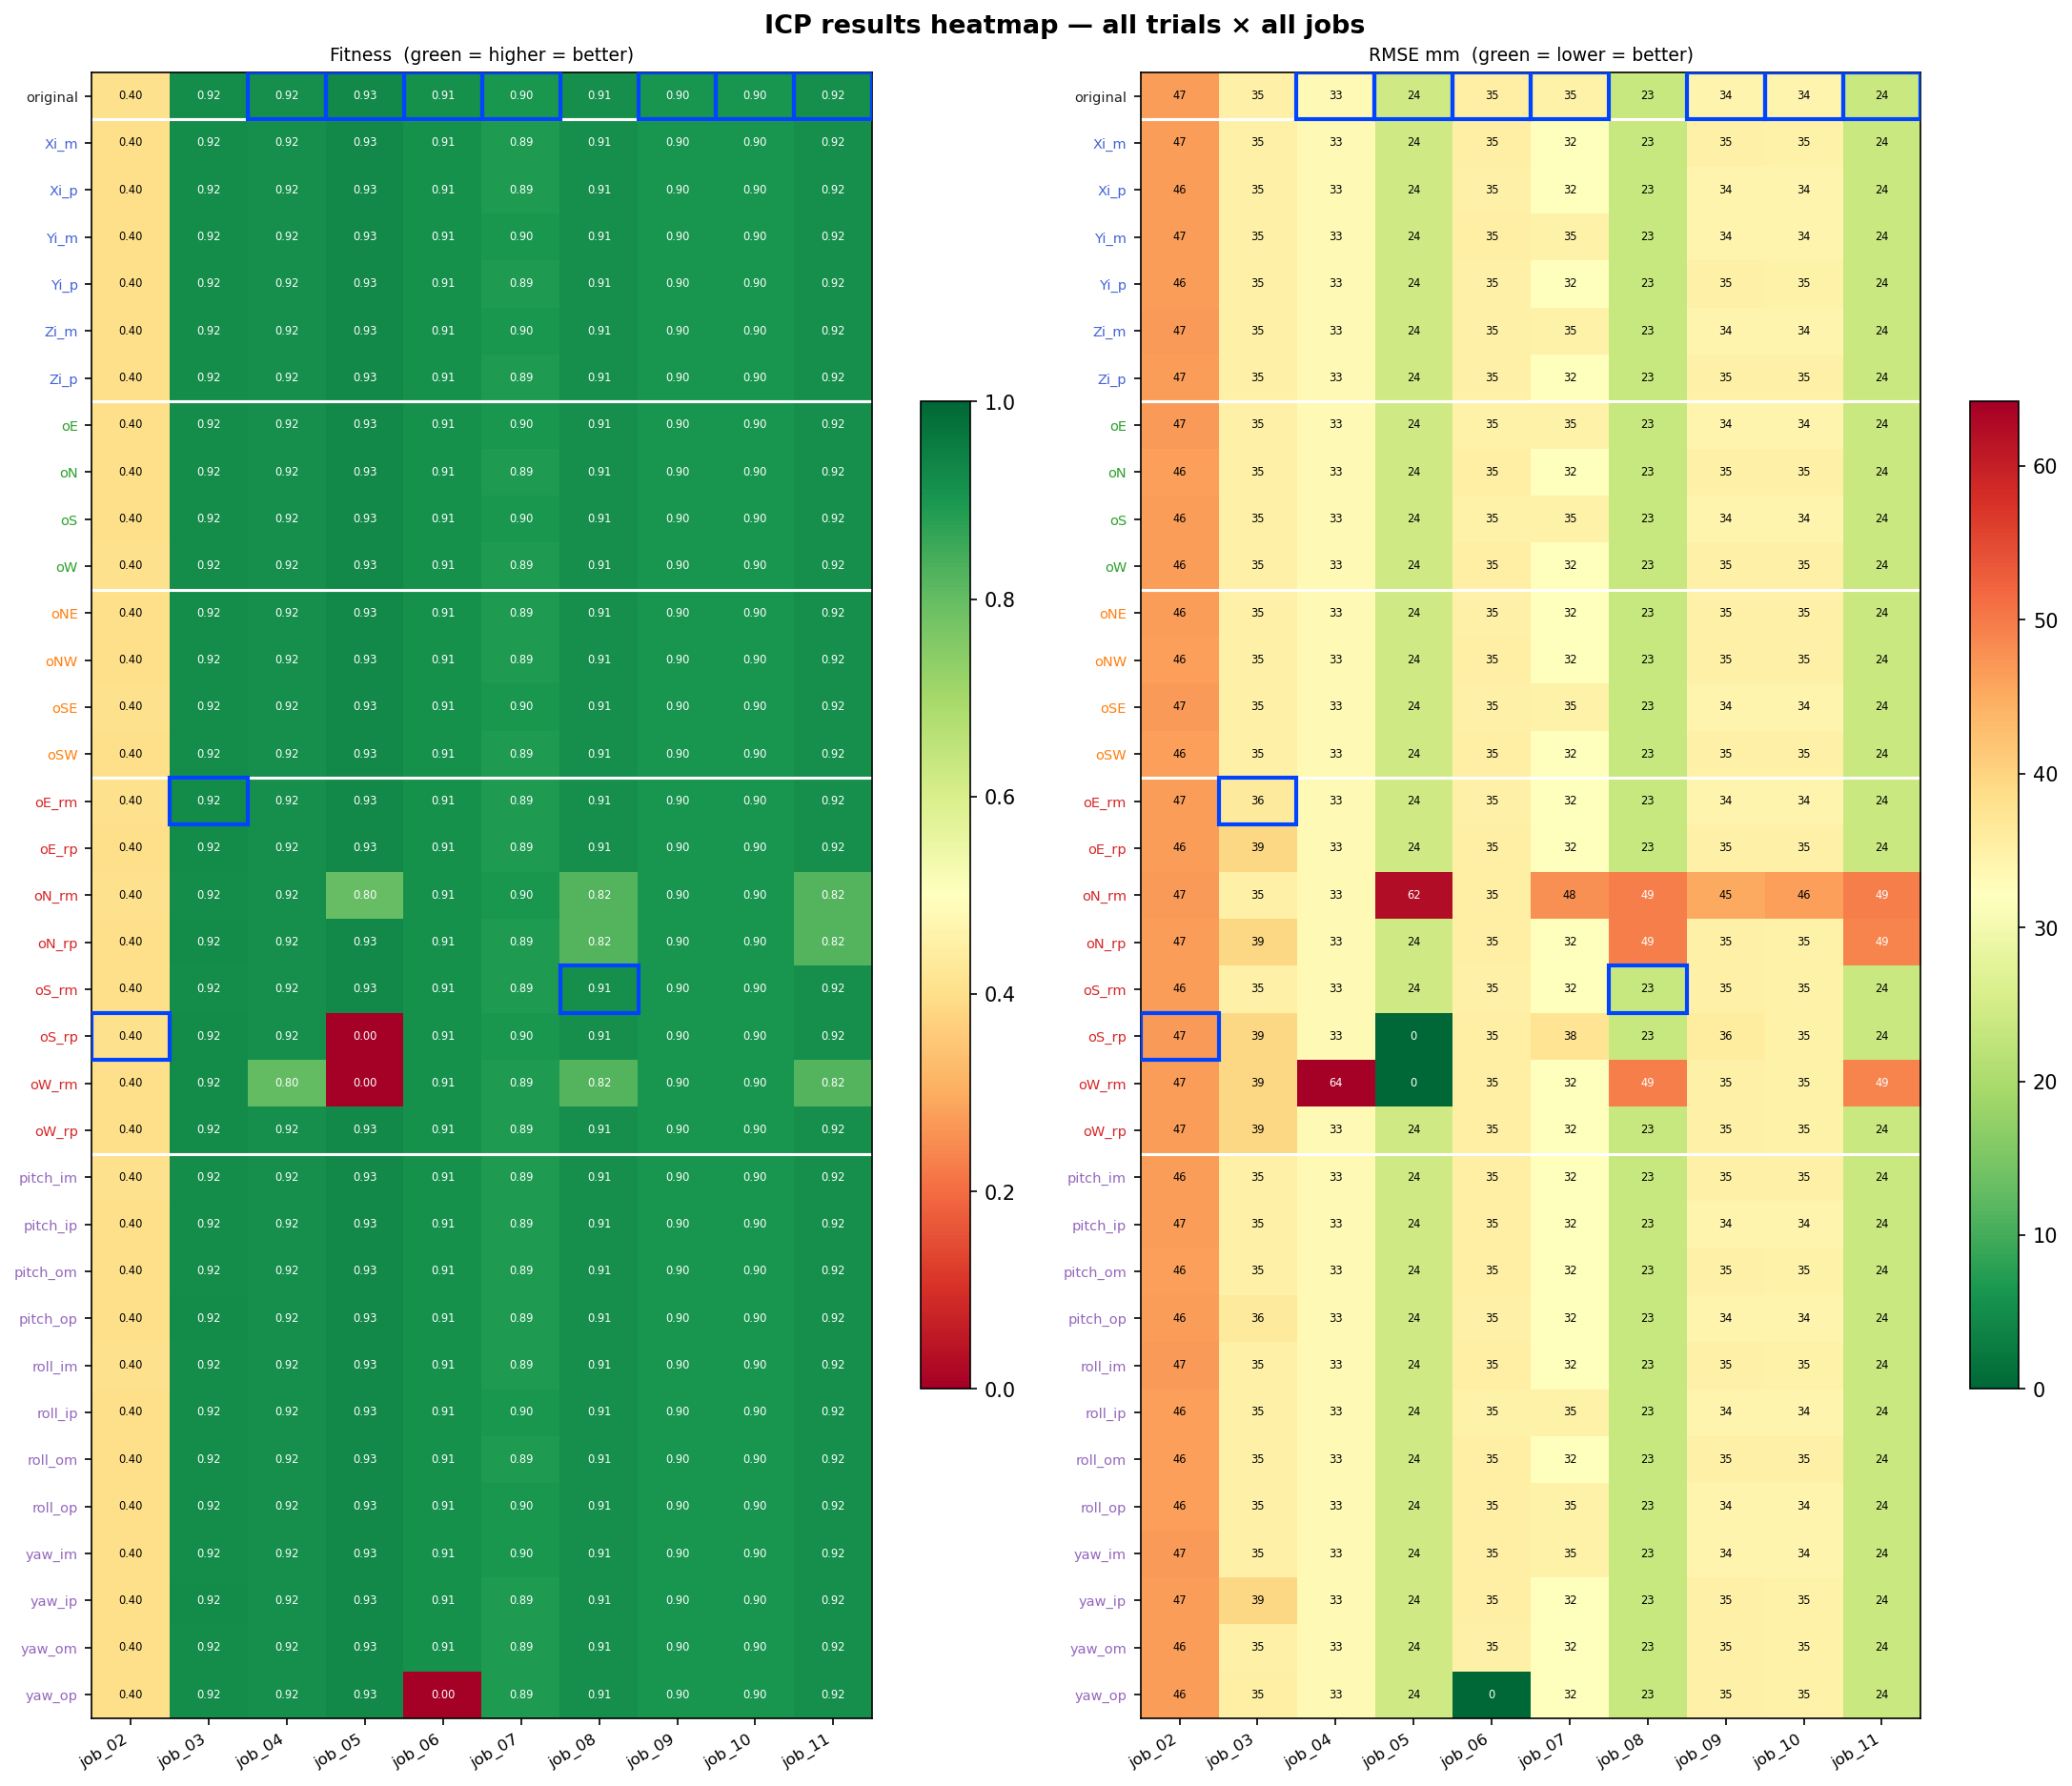
\includegraphics[width=\linewidth]{4-precise-alignment/4-results/figures/lidar_icp_heatmap}
  \caption{ICP fitness heatmap across all hypotheses. Each row corresponds to one condition (ordered by distance); each column to one perturbation hypothesis. Colour intensity indicates fitness score. The D110A0 row visible in this figure was excluded from analysis as it exceeded the stereo pipeline's depth clipping threshold.}
  \label{fig:pa-lidar-heatmap}
\end{figure}

\Cref{fig:pa-lidar-alignment-examples} presents representative alignment visualisations for selected conditions spanning the distance range.

\begin{figure}[htbp]
  \centering
  \begin{subfigure}[b]{0.48\linewidth}
    \centering
    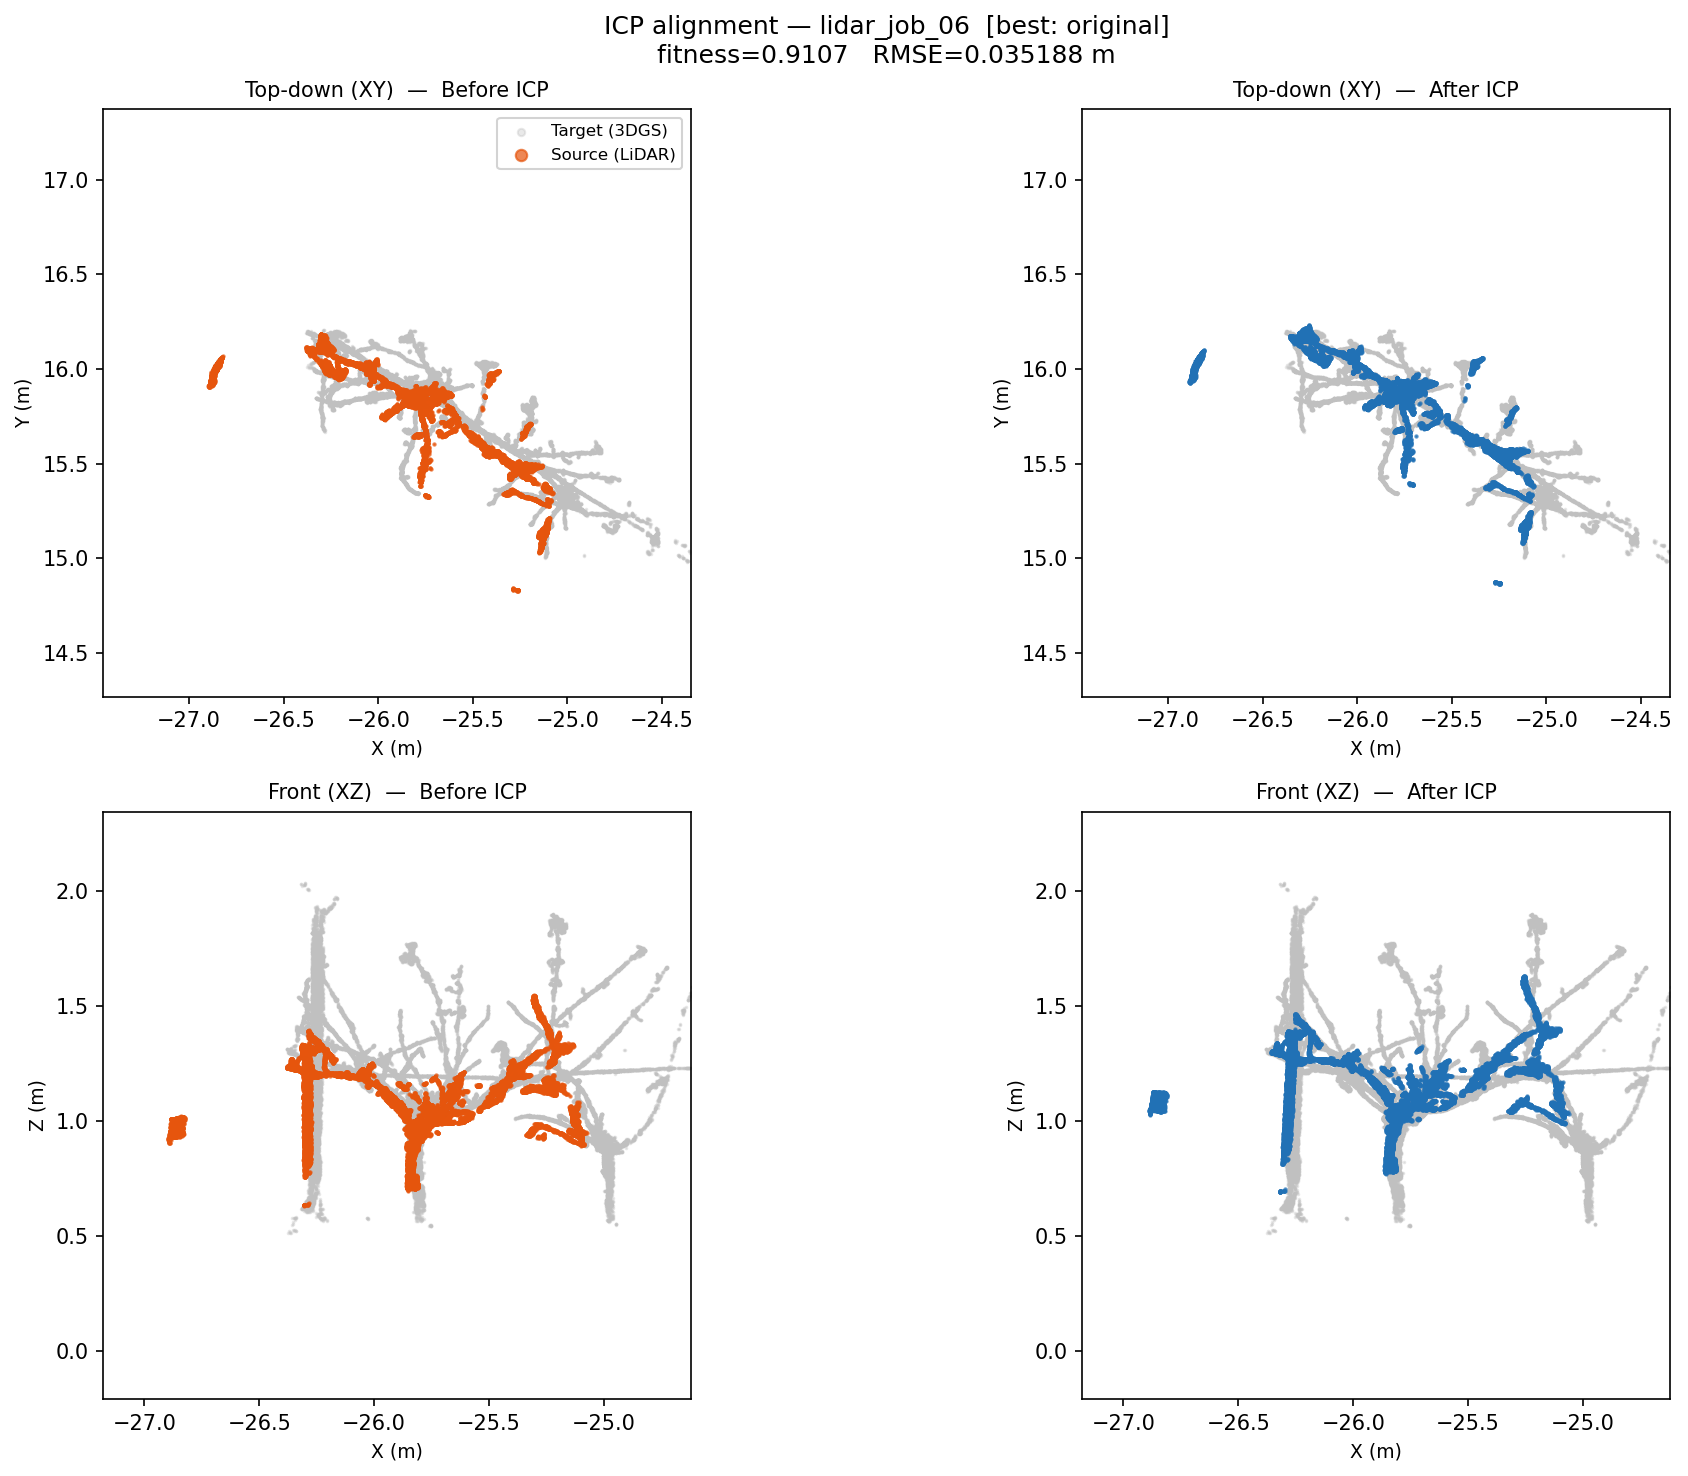
\includegraphics[width=\linewidth]{4-precise-alignment/4-results/figures/lidar_D40A0_alignment}
    \caption{D40A0 (40\,cm, $0^{\circ}$)}
    \label{fig:pa-lidar-align-D40A0}
  \end{subfigure}
  \hfill
  \begin{subfigure}[b]{0.48\linewidth}
    \centering
    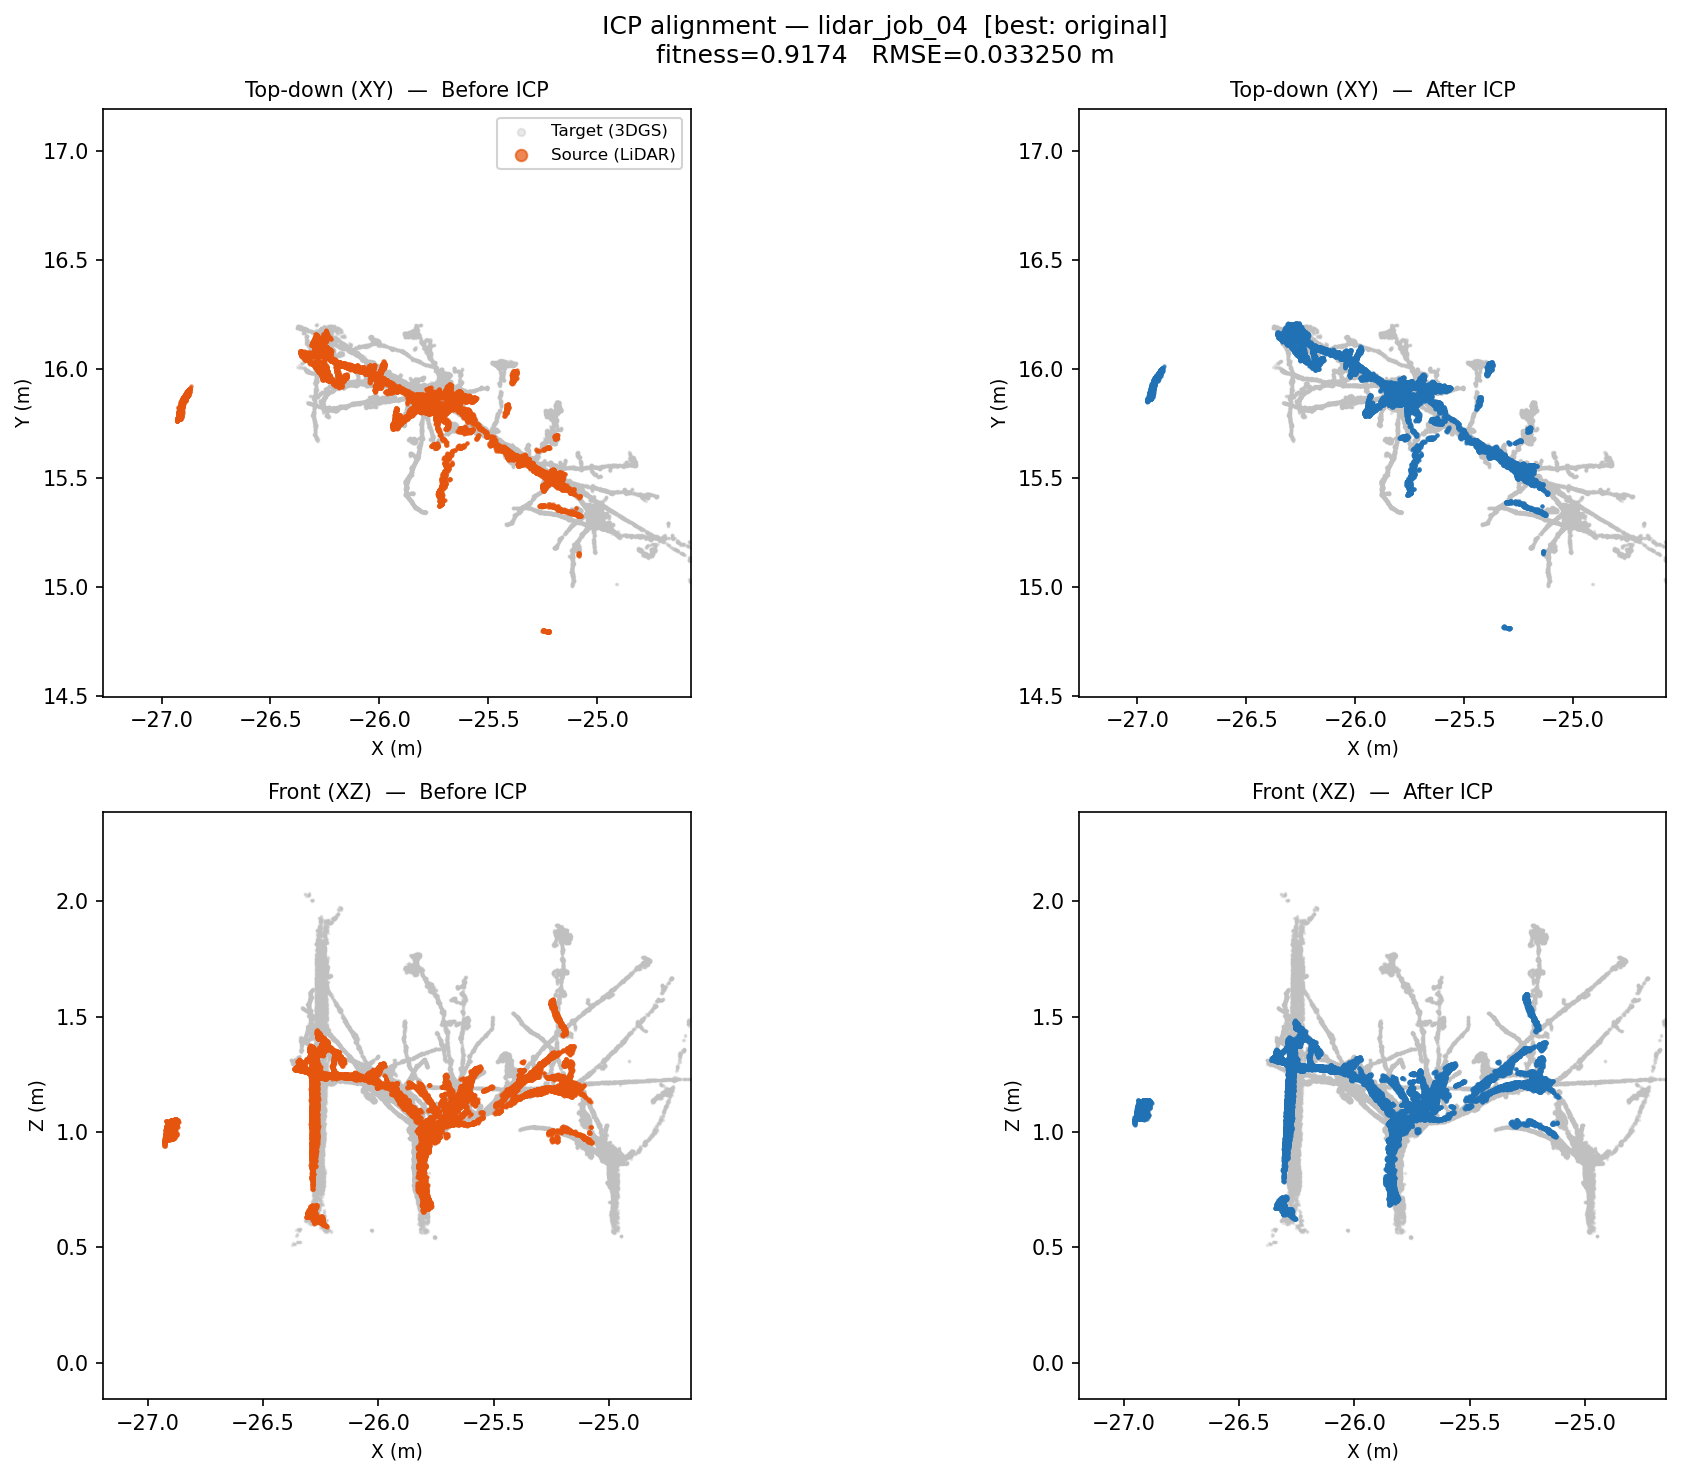
\includegraphics[width=\linewidth]{4-precise-alignment/4-results/figures/lidar_D60A0_alignment}
    \caption{D60A0 (60\,cm, $0^{\circ}$)}
    \label{fig:pa-lidar-align-D60A0}
  \end{subfigure}

  \vspace{0.5em}

  \begin{subfigure}[b]{0.48\linewidth}
    \centering
    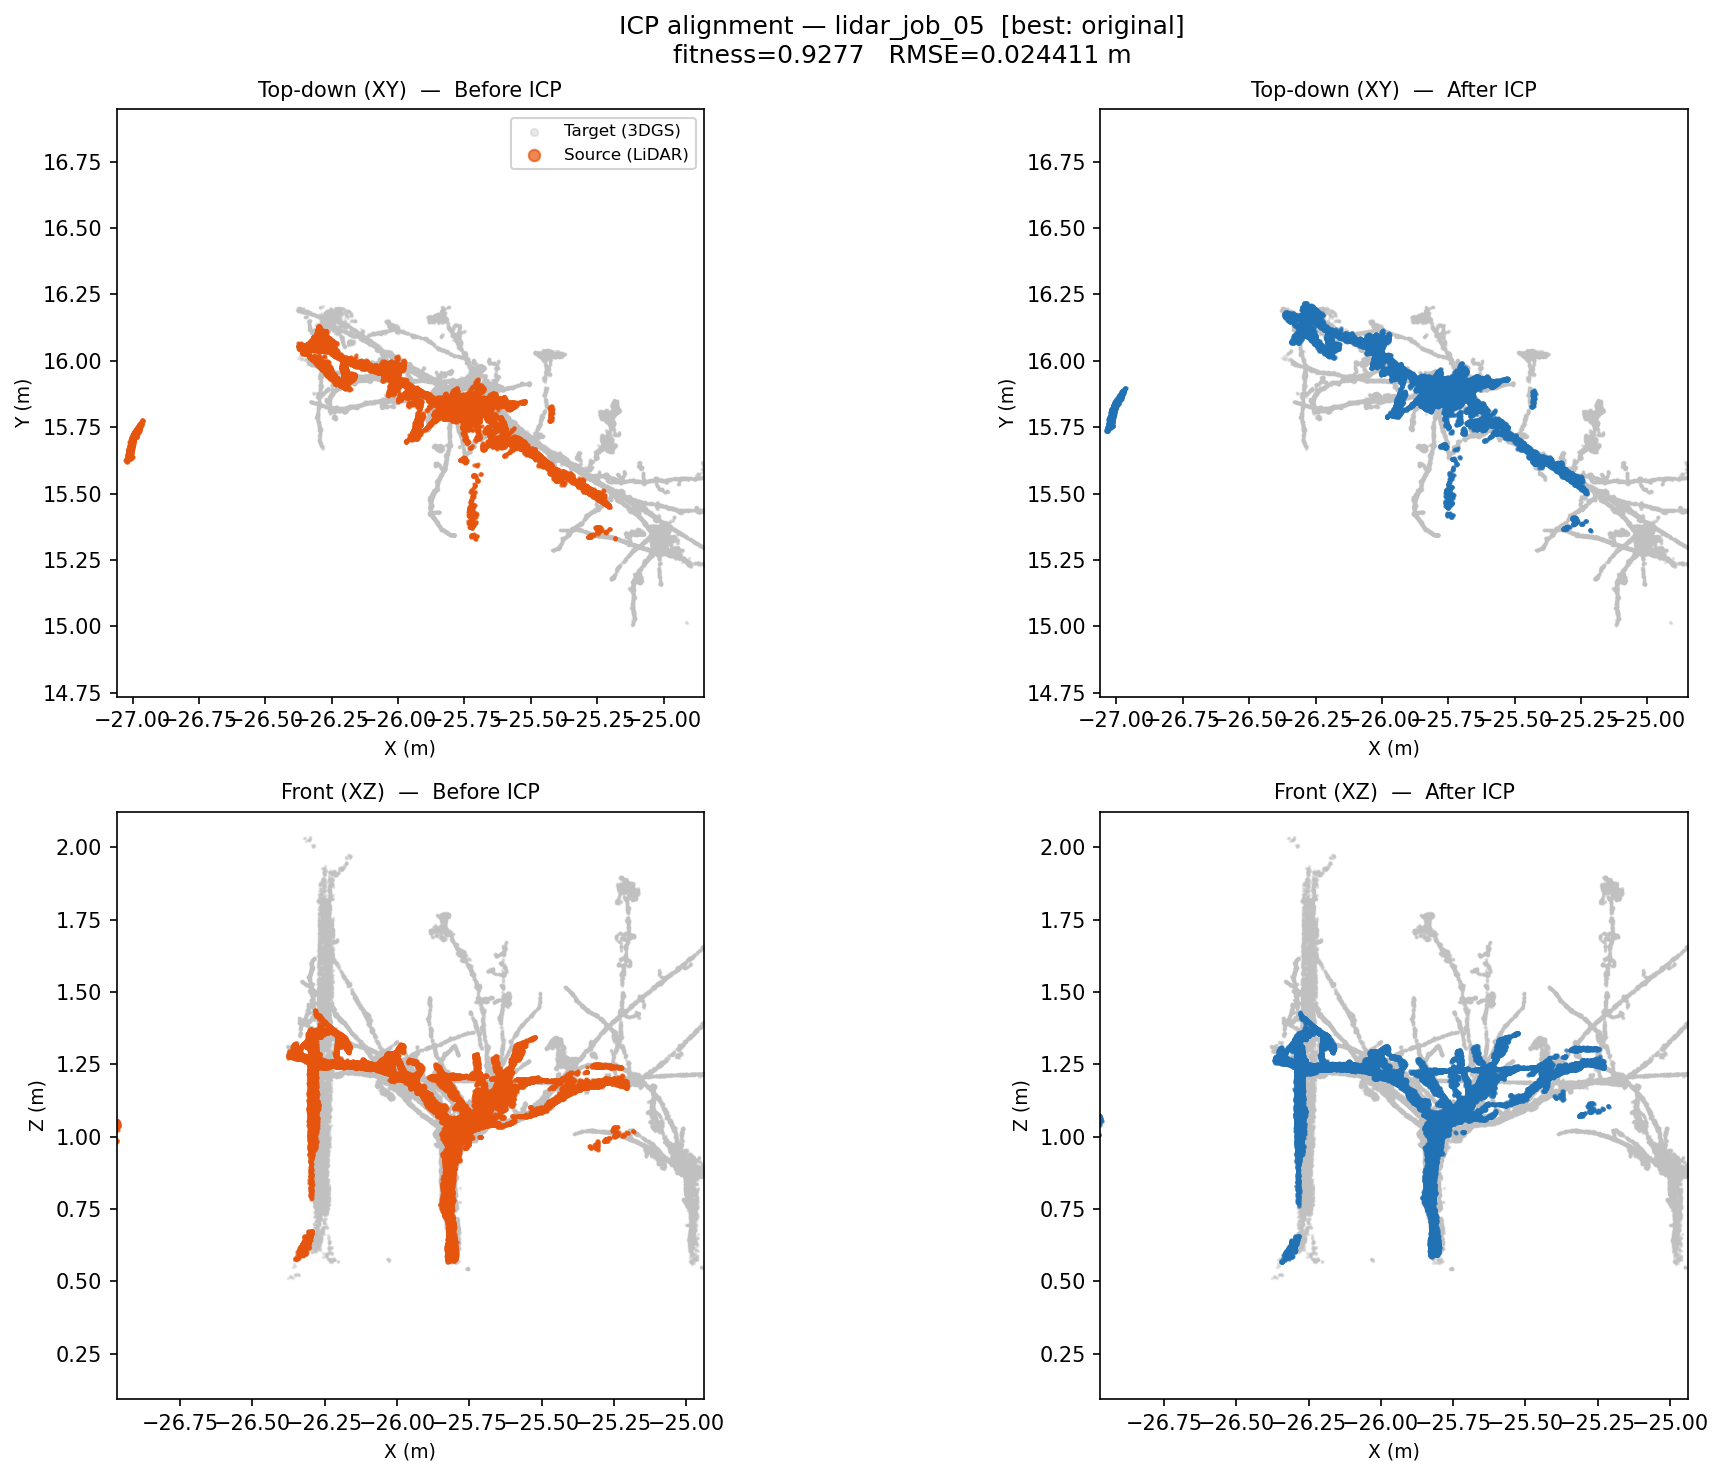
\includegraphics[width=\linewidth]{4-precise-alignment/4-results/figures/lidar_D80A0_alignment}
    \caption{D80A0 (80\,cm, $0^{\circ}$)}
    \label{fig:pa-lidar-align-D80A0}
  \end{subfigure}
  \caption{LiDAR alignment visualisations for the best-selected hypothesis at each $0^{\circ}$ approach angle condition. Source cloud (coloured) overlaid on the 3DGS reference target (grey).}
  \label{fig:pa-lidar-alignment-examples}
\end{figure}

\Cref{fig:pa-lidar-batch-summary} presents the batch summary comparing best-trial registration metrics across all nine conditions.

\begin{figure}[htbp]
  \centering
  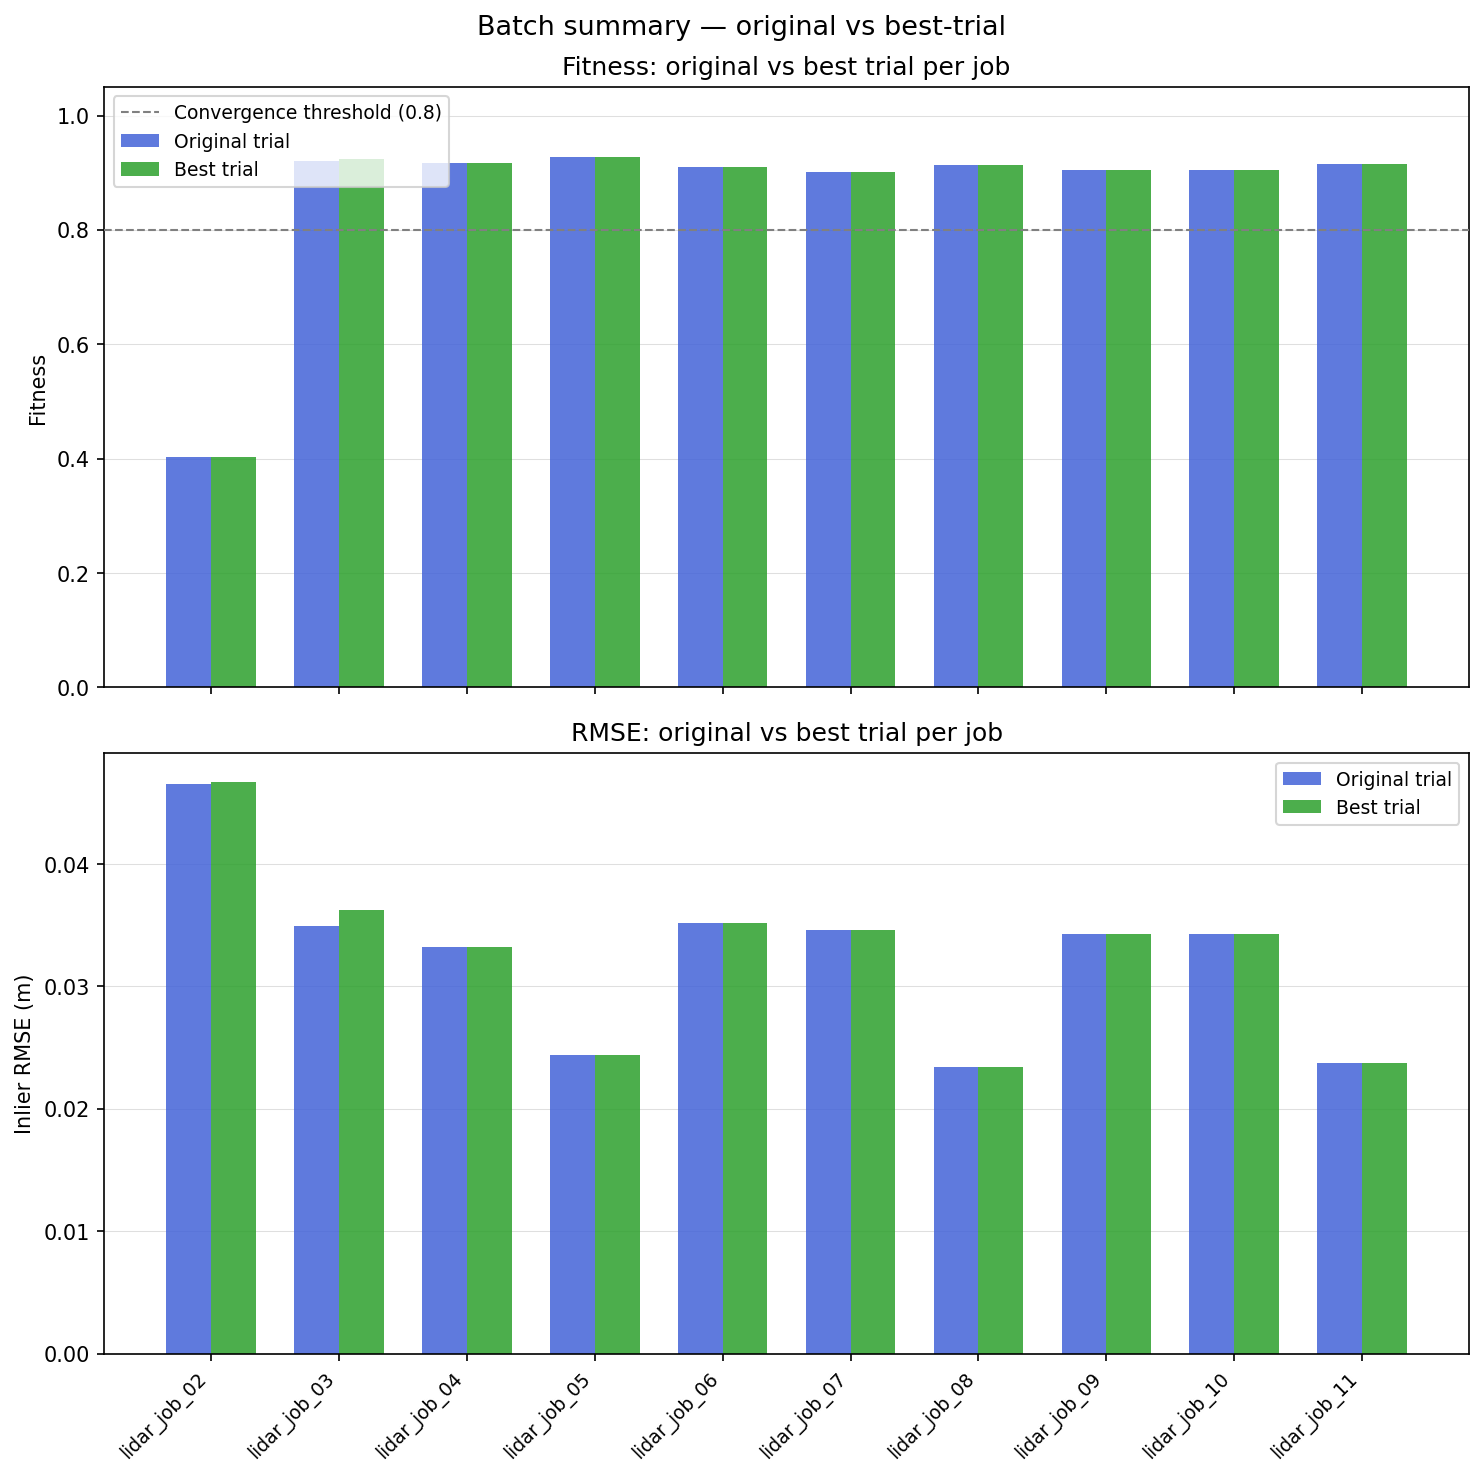
\includegraphics[width=\linewidth]{4-precise-alignment/4-results/figures/lidar_batch_summary}
  \caption{LiDAR batch summary: best-trial fitness and inlier RMSE across all nine conditions. The D110A0 bar visible in this figure was excluded from analysis as it exceeded the stereo pipeline's depth clipping threshold.}
  \label{fig:pa-lidar-batch-summary}
\end{figure}

% ---------------------------------------------------------------------------
\subsection{Stereo Registration Performance}
\label{subsec:pa-results-stereo-summary}
% ---------------------------------------------------------------------------

\Cref{tab:pa-results-stereo-per-condition} summarises the stereo registration outcome for each condition. The stereo pipeline executes a single ICP run per trial; each condition produces exactly one fitness value and one inlier RMSE.

\begin{table}[htbp]
  \centering
  \small
  \setlength{\tabcolsep}{4pt}
  \caption{Per-condition stereo registration summary. Fitness takes a binary value (1.0 or 0.0) because the stereo pipeline executes a single ICP run. Non-converging conditions are listed with dashes for RMSE. All RMSE values in millimetres.}
  \label{tab:pa-results-stereo-per-condition}
  \begin{tabular}{@{} l r r r r r @{}}
    \toprule
    \textbf{Condition} &
    \textbf{Raw pts} &
    \textbf{Proc.\ pts} &
    \boldmath$F$ &
    \boldmath$\varepsilon$ \textbf{(mm)} &
    \textbf{Total time (s)} \\
    \midrule
    D40A$-$15 &  99\,661 & 87\,772 & 1.0 & 16.77 & 14.76 \\
    D40A0     &  97\,181 & 83\,163 & 1.0 & 16.77 & 13.13 \\
    D40A$+$15 &  99\,661 & 87\,994 & 0.0 &  ---  & 11.85 \\
    D60A$-$15 & 107\,944 & 91\,952 & 1.0 & 16.67 & 13.33 \\
    D60A0     &  93\,336 & 68\,811 & 1.0 & 16.76 & 15.08 \\
    D60A$+$15 &  99\,661 & 87\,666 & 1.0 & 16.67 & 12.66 \\
    D80A$-$15 &  81\,464 & 23\,980 & 0.0 &  ---  & 11.82 \\
    D80A0     &  84\,748 & 42\,307 & 1.0 & 12.26 & 20.28 \\
    D80A$+$15 &  81\,464 & 29\,981 & 1.0 & 12.64 & 14.69 \\
    \bottomrule
  \end{tabular}
\end{table}

Seven of nine conditions converged (78\%). Two conditions failed: D40A$+$15 (87\,994 processed points, $F = 0.0$) and D80A$-$15 (23\,980 processed points, $F = 0.0$).

% ---------------------------------------------------------------------------
\subsection{Stereo: Distance and Angle Effects}
\label{subsec:pa-results-stereo-distance-angle}
% ---------------------------------------------------------------------------

\Cref{tab:pa-results-stereo-by-distance,tab:pa-results-stereo-by-angle} present stereo registration outcomes grouped by distance and angle.

\begin{table}[htbp]
  \centering
  \caption{Stereo registration results grouped by sensor-to-vine distance. RMSE computed over converging conditions only. All values in millimetres.}
  \label{tab:pa-results-stereo-by-distance}
  \begin{tabular}{@{} l r r r @{}}
    \toprule
    \textbf{Distance} &
    \textbf{Converged / Total} &
    \textbf{Conv.\ rate (\%)} &
    \textbf{Median} \boldmath$\varepsilon$ \textbf{(mm)} \\
    \midrule
    D40 (40\,cm)   & 2/3 &  67 & 16.77 \\
    D60 (60\,cm)   & 3/3 & 100 & 16.67 \\
    D80 (80\,cm)   & 2/3 &  67 & 12.45 \\
    \bottomrule
  \end{tabular}
\end{table}

\begin{table}[htbp]
  \centering
  \caption{Stereo registration results grouped by approach angle. RMSE computed over converging conditions only. All values in millimetres.}
  \label{tab:pa-results-stereo-by-angle}
  \begin{tabular}{@{} l r r r @{}}
    \toprule
    \textbf{Angle} &
    \textbf{Converged / Total} &
    \textbf{Conv.\ rate (\%)} &
    \textbf{Median} \boldmath$\varepsilon$ \textbf{(mm)} \\
    \midrule
    A$-$15 ($-15^{\circ}$) & 2/3 &  67 & 16.72 \\
    A0 ($0^{\circ}$)       & 3/3 & 100 & 16.76 \\
    A$+$15 ($+15^{\circ}$) & 2/3 &  67 & 14.66 \\
    \bottomrule
  \end{tabular}
\end{table}

D60 achieved full convergence (3/3). The D80 group exhibits lower RMSE (12.45\,mm) compared to D40 (16.77\,mm) and D60 (16.67\,mm). Convergence rates range from 67\% (A$-$15, A$+$15) to 100\% (A0).

% ---------------------------------------------------------------------------
\subsection{Stereo: Recovered ICP Correction}
\label{subsec:pa-results-stereo-transformation}
% ---------------------------------------------------------------------------

\Cref{tab:pa-results-stereo-transforms} reports the positional displacement and rotation correction applied by the GICP solver for each converging condition. The translational displacement $\lVert\Delta\mathbf{t}\rVert$ is the Euclidean distance between the initial and final sensor positions; component displacements ($\Delta x$, $\Delta y$, $\Delta z$) are in the local ENU frame. Rotations are ZYX Euler angles extracted from the correction matrix.

\begin{table}[htbp]
  \centering
  \small
  \setlength{\tabcolsep}{3pt}
  \caption{ICP correction for converging stereo conditions. Translational displacement in millimetres; rotation corrections as ZYX Euler angles in degrees. Non-converging conditions (D80A$-$15, D40A$+$15) omitted.}
  \label{tab:pa-results-stereo-transforms}
  \begin{tabular}{@{} l r r r r r r r @{}}
    \toprule
    \textbf{Condition} &
    \boldmath$\lVert\Delta\mathbf{t}\rVert$ \textbf{(mm)} &
    \boldmath$\Delta x$ \textbf{(mm)} &
    \boldmath$\Delta y$ \textbf{(mm)} &
    \boldmath$\Delta z$ \textbf{(mm)} &
    \boldmath$\Delta\psi$ \textbf{(°)} &
    \boldmath$\Delta\theta$ \textbf{(°)} &
    \boldmath$\Delta\phi$ \textbf{(°)} \\
    \midrule
    D40A$-$15 &  86.3 & $-$17.5 &    76.8 &    35.4 & $-$1.65 &    0.67 & $-$2.46 \\
    D40A0     &  67.5 &    44.4 &    47.8 &    17.2 &    2.25 & $-$1.15 & $-$3.43 \\
    D60A$-$15 & 117.7 & $-$34.6 &   106.3 &    36.9 & $-$3.85 & $-$0.34 & $-$4.15 \\
    D60A0     &  63.7 & $-$23.5 &    48.9 &    33.4 & $-$2.12 & $-$1.48 & $-$3.36 \\
    D60A$+$15 &  46.6 &     8.1 &    35.0 &    29.6 & $-$1.21 &    0.73 & $-$3.08 \\
    D80A0     & 140.6 &  $-$5.2 &    79.9 &   115.6 & $-$0.74 & $-$3.24 & $-$6.60 \\
    D80A$+$15 &  91.4 & $-$22.5 &    63.2 &    62.1 & $-$2.69 & $-$4.49 & $-$3.77 \\
    \bottomrule
  \end{tabular}
\end{table}

For the seven converging conditions, the mean positional displacement is 87.7\,mm (max 140.6\,mm, D80A0), confirming that ICP adjustments remain within the expected range of the initial pose estimate. The roll correction ($\Delta\phi$) is consistently negative, ranging from $-2.5^{\circ}$ to $-6.6^{\circ}$. Rotational corrections are smaller than the LiDAR equivalents, with all angles below $6.6^{\circ}$.

% ---------------------------------------------------------------------------
\subsection{Stereo: Pipeline Timing}
\label{subsec:pa-results-stereo-timing}
% ---------------------------------------------------------------------------

\Cref{tab:pa-results-stereo-timing} reports wall-clock timing for each stereo trial, decomposed into four stages: depth estimation (FoundationStereo inference and back-projection), dual-camera combination, preprocessing (morphological closing, DBSCAN, voxel density filtering), and ICP alignment.

\begin{table}[htbp]
  \centering
  \small
  \setlength{\tabcolsep}{4pt}
  \caption{Per-condition stereo pipeline timing. All values in seconds. No scan accumulation interval precedes the pipeline.}
  \label{tab:pa-results-stereo-timing}
  \begin{tabular}{@{} l r r r r r @{}}
    \toprule
    \textbf{Condition} &
    \textbf{Depth (s)} &
    \textbf{Combine (s)} &
    \textbf{Process (s)} &
    \textbf{ICP (s)} &
    \textbf{Total (s)} \\
    \midrule
    D40A$-$15 & 1.25 & 4.46 & 1.08 &  7.96 & 14.76 \\
    D40A0     & 1.24 & 4.51 & 0.94 &  6.44 & 13.13 \\
    D40A$+$15 & 1.25 & 4.46 & 1.10 &  5.04 & 11.85 \\
    D60A$-$15 & 1.26 & 4.42 & 1.02 &  6.64 & 13.33 \\
    D60A0     & 1.23 & 4.72 & 0.88 &  8.25 & 15.08 \\
    D60A$+$15 & 1.24 & 4.68 & 1.10 &  5.64 & 12.66 \\
    D80A$-$15 & 1.20 & 4.61 & 0.86 &  5.15 & 11.82 \\
    D80A0     & 1.20 & 4.94 & 0.78 & 13.36 & 20.28 \\
    D80A$+$15 & 1.20 & 4.61 & 0.71 &  8.17 & 14.69 \\
    \midrule
    \textbf{Mean $\pm$ std} & $1.23 \pm 0.02$ & $4.60 \pm 0.16$ & $0.94 \pm 0.14$ & $7.41 \pm 2.56$ & $14.18 \pm 2.59$ \\
    \bottomrule
  \end{tabular}
\end{table}

Total pipeline latency ranges from 11.82\,s (D80A$-$15) to 20.28\,s (D80A0), with a mean of $14.18 \pm 2.59$\,s. Depth estimation is consistent at approximately 1.2\,s. The dominant timing components are dual-camera combination ($4.60 \pm 0.16$\,s) and ICP alignment ($7.41 \pm 2.56$\,s).

% ---------------------------------------------------------------------------
\subsection{Stereo: Visual Alignment}
\label{subsec:pa-results-stereo-visual}
% ---------------------------------------------------------------------------

\Cref{fig:pa-stereo-icp-comparison} presents before-and-after ICP alignment comparisons for a representative converging condition (D80A0) and a representative non-converging condition (D40A$+$15).

\begin{figure}[htbp]
  \centering
  \begin{subfigure}[b]{0.48\linewidth}
    \centering
    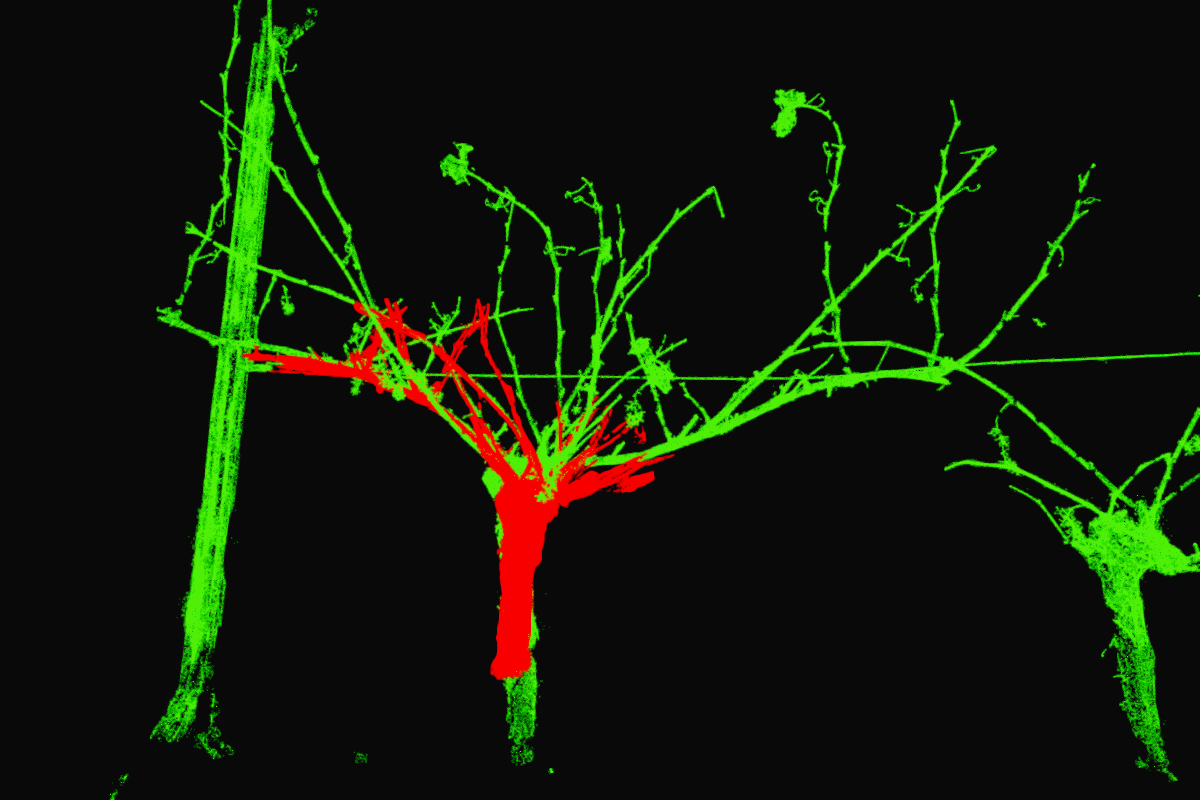
\includegraphics[width=\linewidth]{4-precise-alignment/4-results/figures/stereo_D80A0_4b_icp_initial_side}
    \caption{D80A0: before registration.}
    \label{fig:stereo-D80A0-initial}
  \end{subfigure}
  \hfill
  \begin{subfigure}[b]{0.48\linewidth}
    \centering
    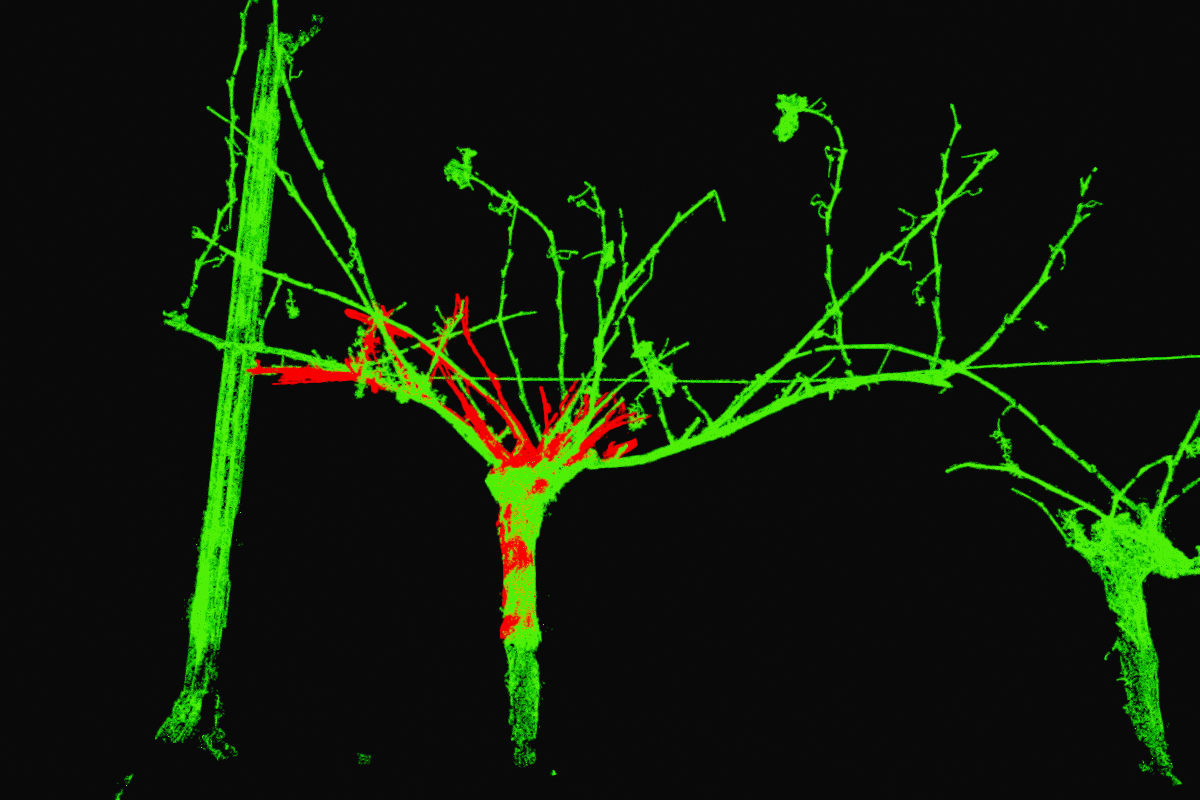
\includegraphics[width=\linewidth]{4-precise-alignment/4-results/figures/stereo_D80A0_5b_icp_final_side}
    \caption{D80A0: after registration ($\varepsilon = 12.26$\,mm).}
    \label{fig:stereo-D80A0-final}
  \end{subfigure}

  \vspace{0.5em}

  \begin{subfigure}[b]{0.48\linewidth}
    \centering
    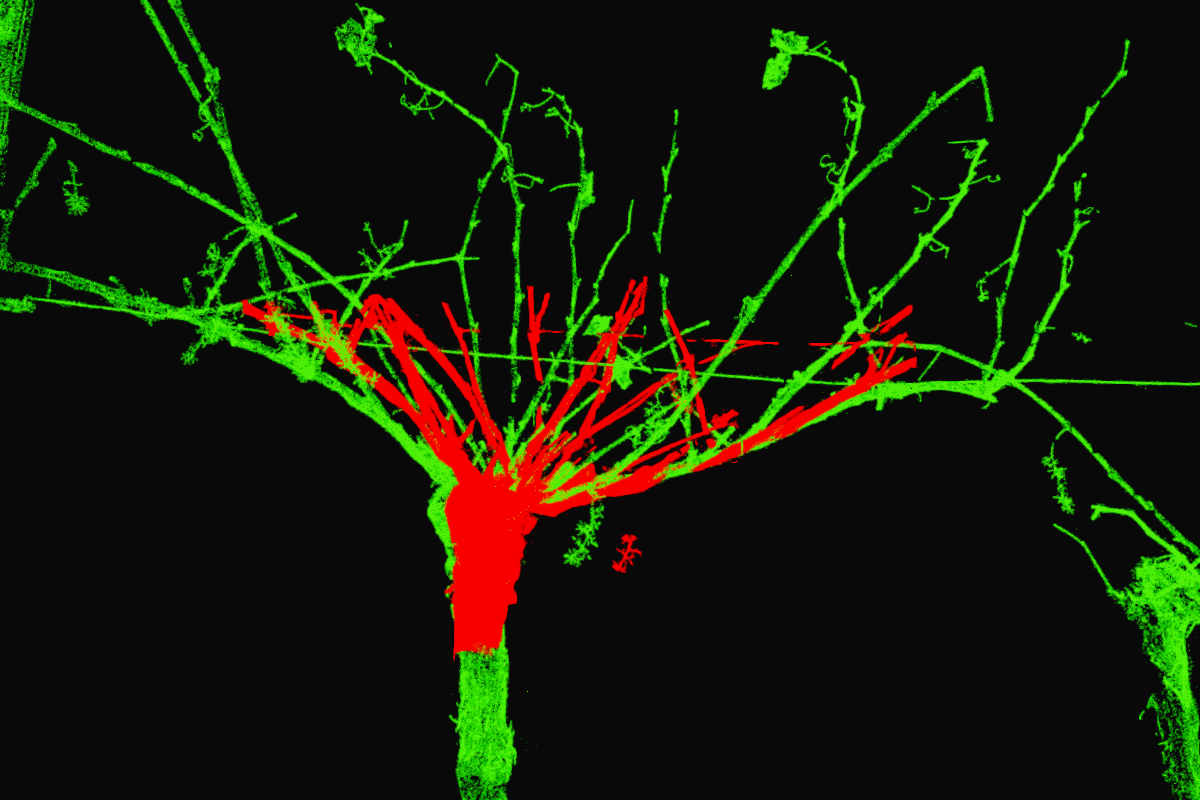
\includegraphics[width=\linewidth]{4-precise-alignment/4-results/figures/stereo_D40Ap15_4b_icp_initial_side}
    \caption{D40A$+$15: before registration.}
    \label{fig:stereo-D40Ap15-initial}
  \end{subfigure}
  \hfill
  \begin{subfigure}[b]{0.48\linewidth}
    \centering
    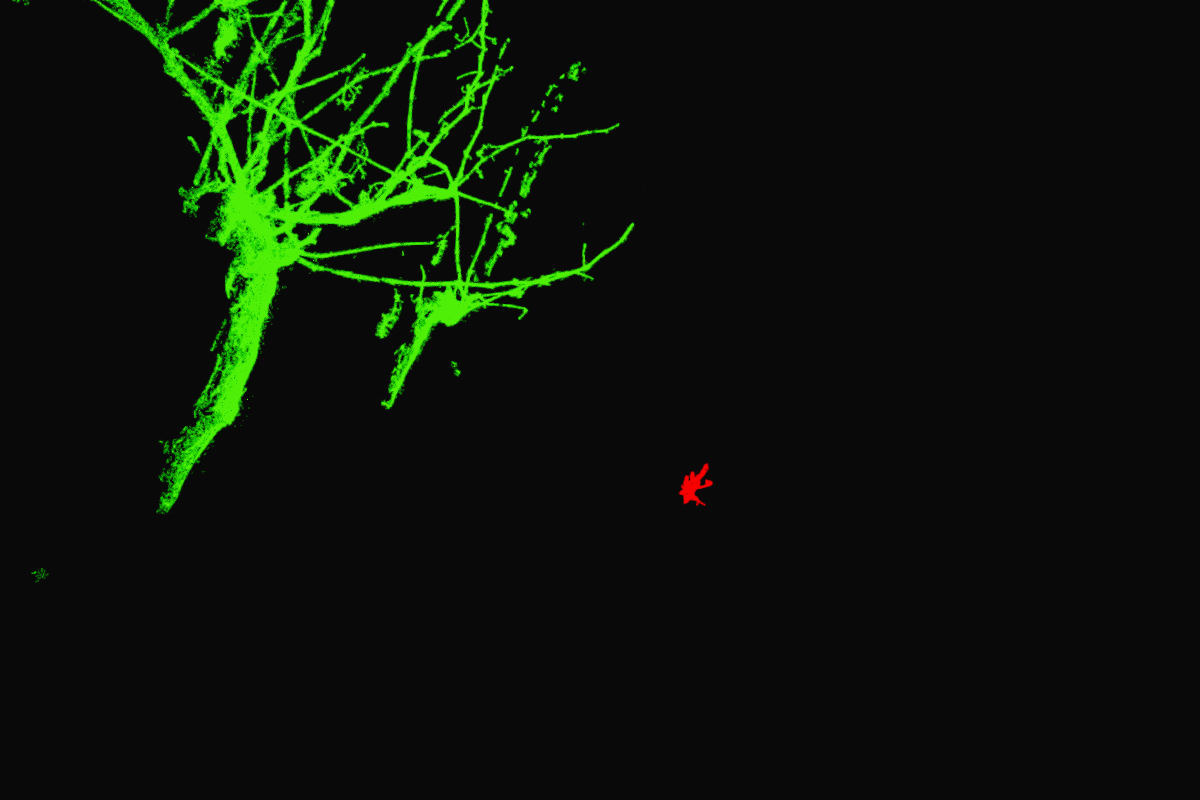
\includegraphics[width=\linewidth]{4-precise-alignment/4-results/figures/stereo_D40Ap15_5b_icp_final_side}
    \caption{D40A$+$15: after registration (failed, $F = 0.0$).}
    \label{fig:stereo-D40Ap15-final}
  \end{subfigure}
  \caption{Stereo ICP alignment comparison (vine-face view). Top row: D80A0, a converging trial achieving 12.26\,mm RMSE. Bottom row: D40A$+$15, a non-converging trial. Green: 3DGS reference cloud; red: stereo source cloud.}
  \label{fig:pa-stereo-icp-comparison}
\end{figure}

\Cref{fig:pa-stereo-converged-overlay} presents the final alignment for all seven converging conditions.

\begin{figure}[htbp]
  \centering
  \begin{subfigure}[b]{0.32\linewidth}
    \centering
    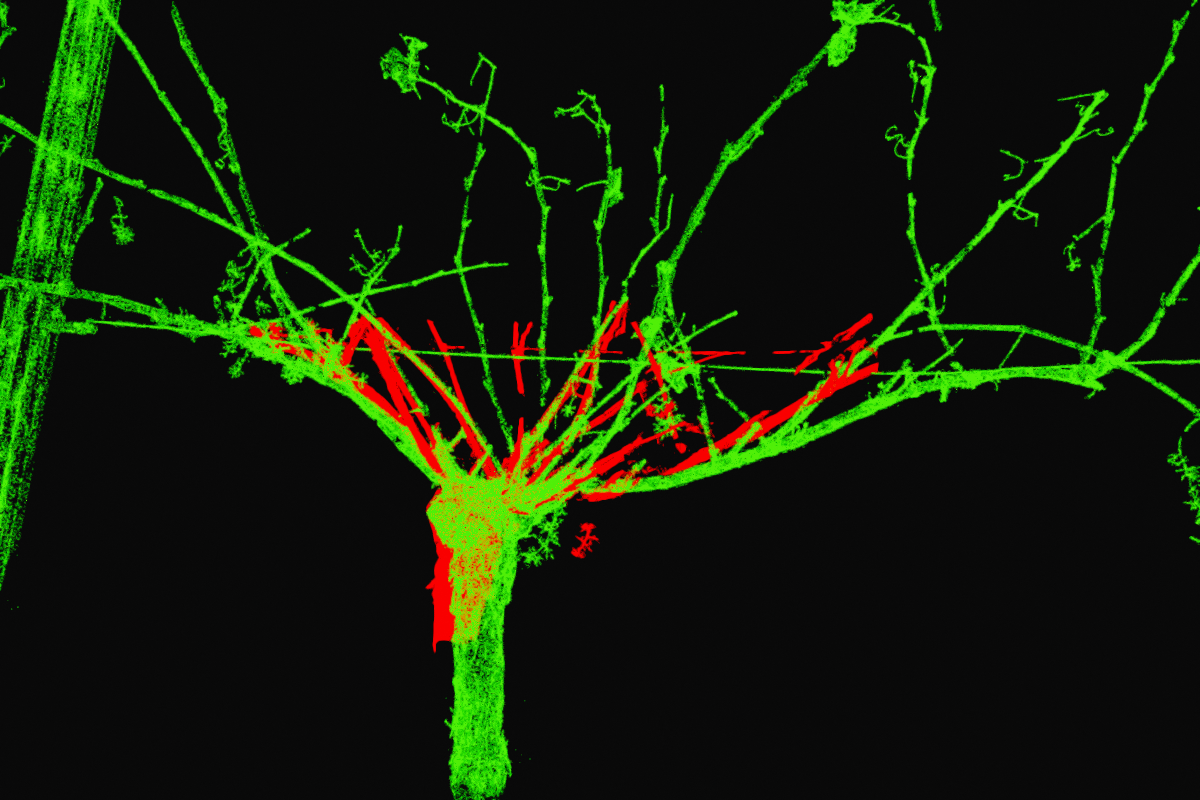
\includegraphics[width=\linewidth]{4-precise-alignment/4-results/figures/stereo_D40Am15_5b_icp_final_side}
    \caption{D40A$-$15}
  \end{subfigure}
  \hfill
  \begin{subfigure}[b]{0.32\linewidth}
    \centering
    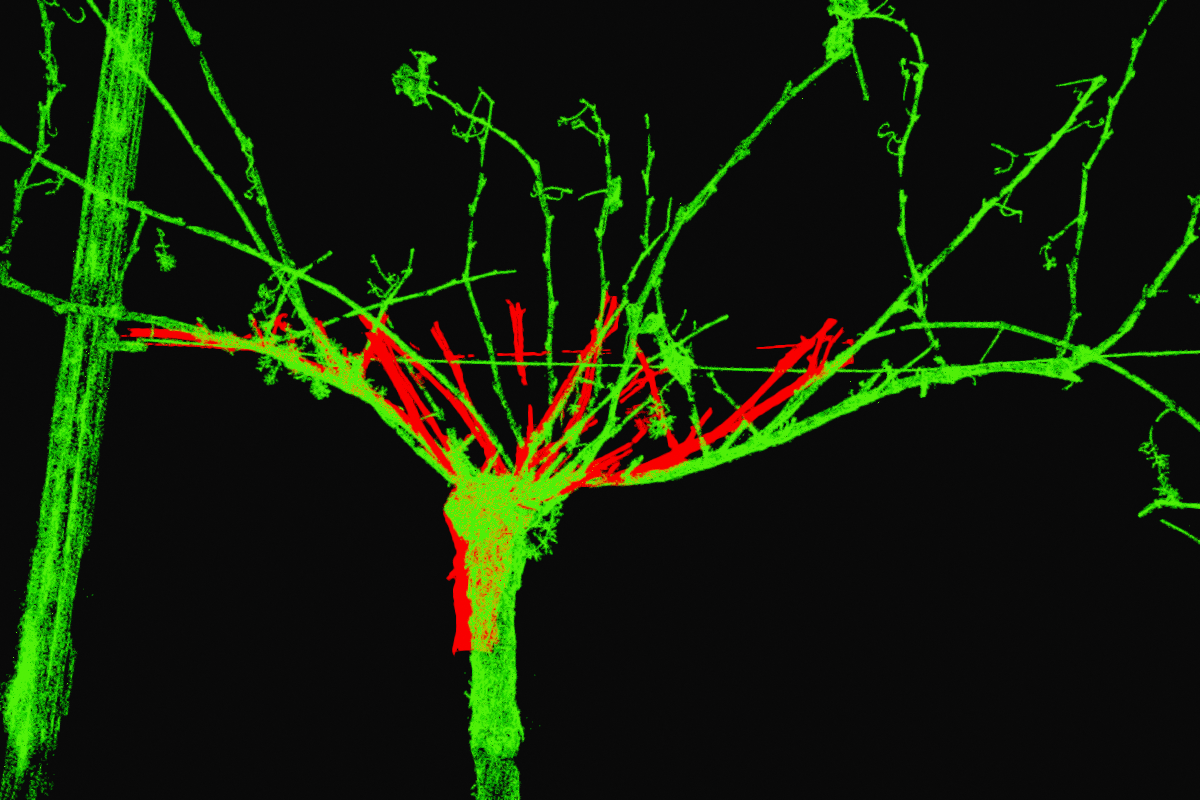
\includegraphics[width=\linewidth]{4-precise-alignment/4-results/figures/stereo_D40A0_5b_icp_final_side}
    \caption{D40A0}
  \end{subfigure}
  \hfill
  \begin{subfigure}[b]{0.32\linewidth}
    \centering
    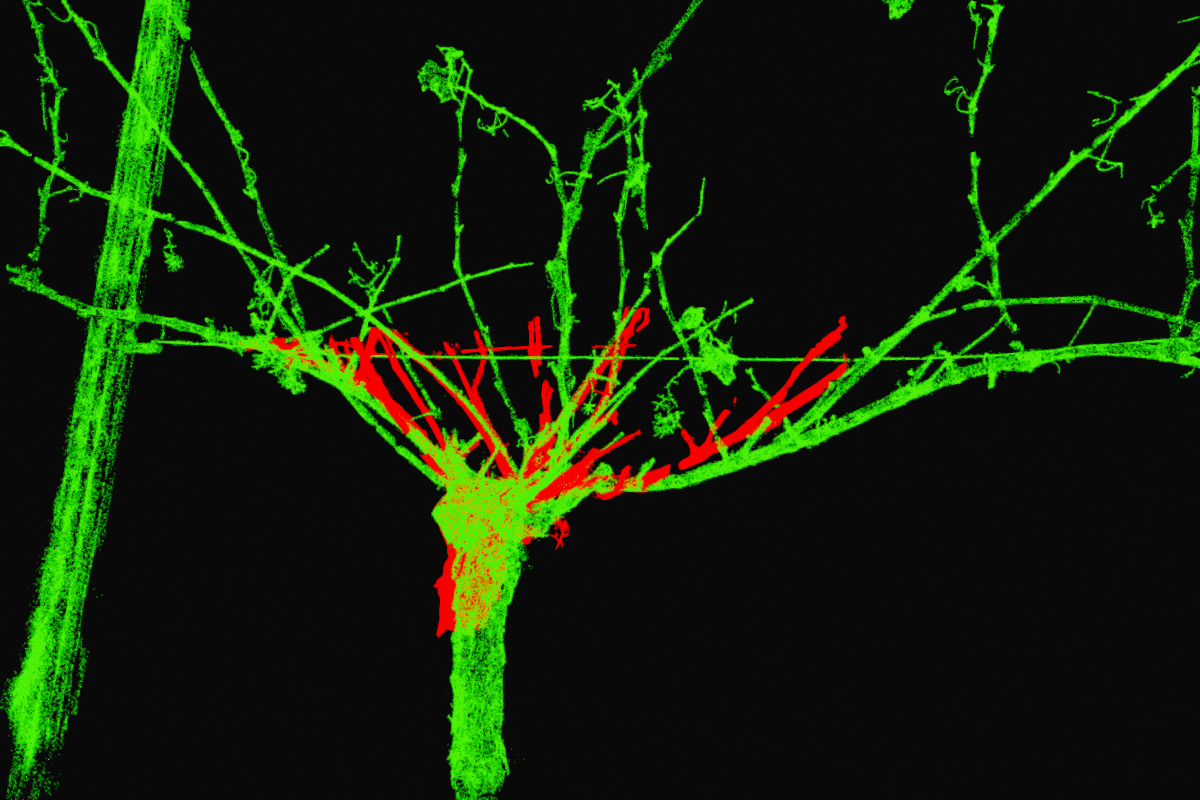
\includegraphics[width=\linewidth]{4-precise-alignment/4-results/figures/stereo_D60Am15_5b_icp_final_side}
    \caption{D60A$-$15}
  \end{subfigure}

  \vspace{0.5em}

  \begin{subfigure}[b]{0.32\linewidth}
    \centering
    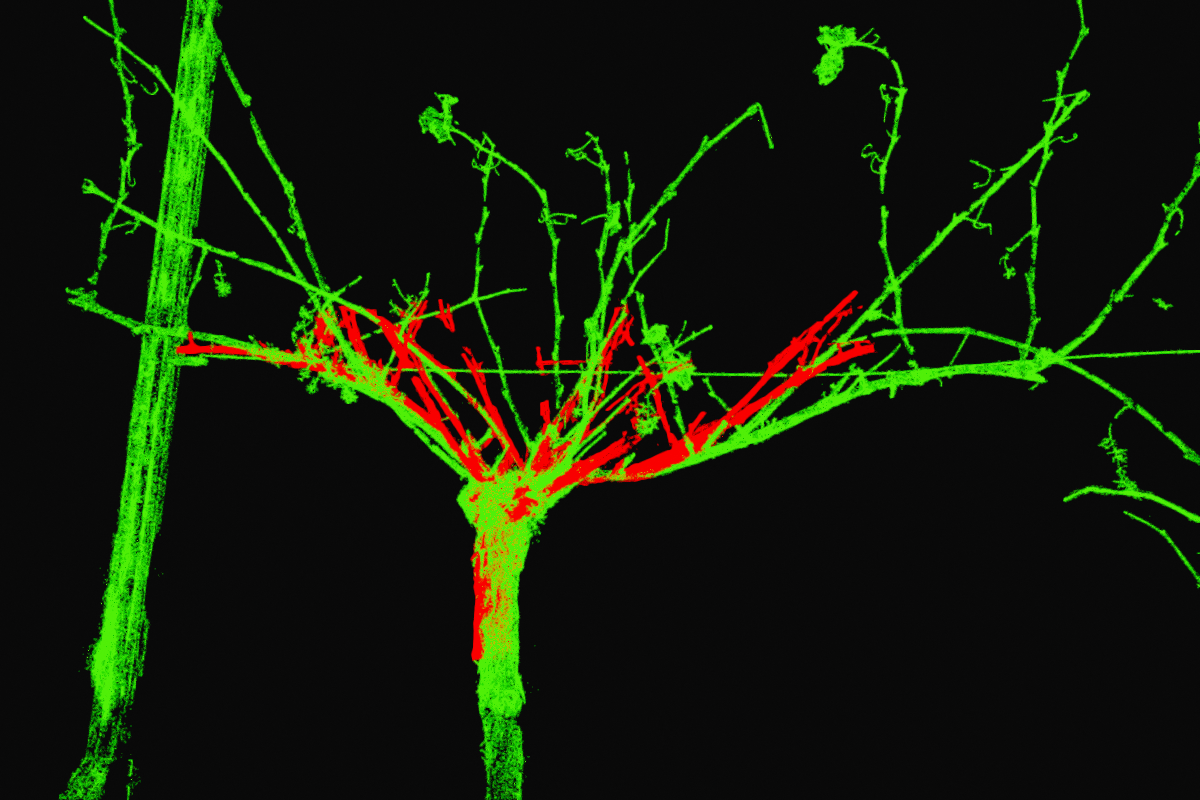
\includegraphics[width=\linewidth]{4-precise-alignment/4-results/figures/stereo_D60A0_5b_icp_final_side}
    \caption{D60A0}
  \end{subfigure}
  \hfill
  \begin{subfigure}[b]{0.32\linewidth}
    \centering
    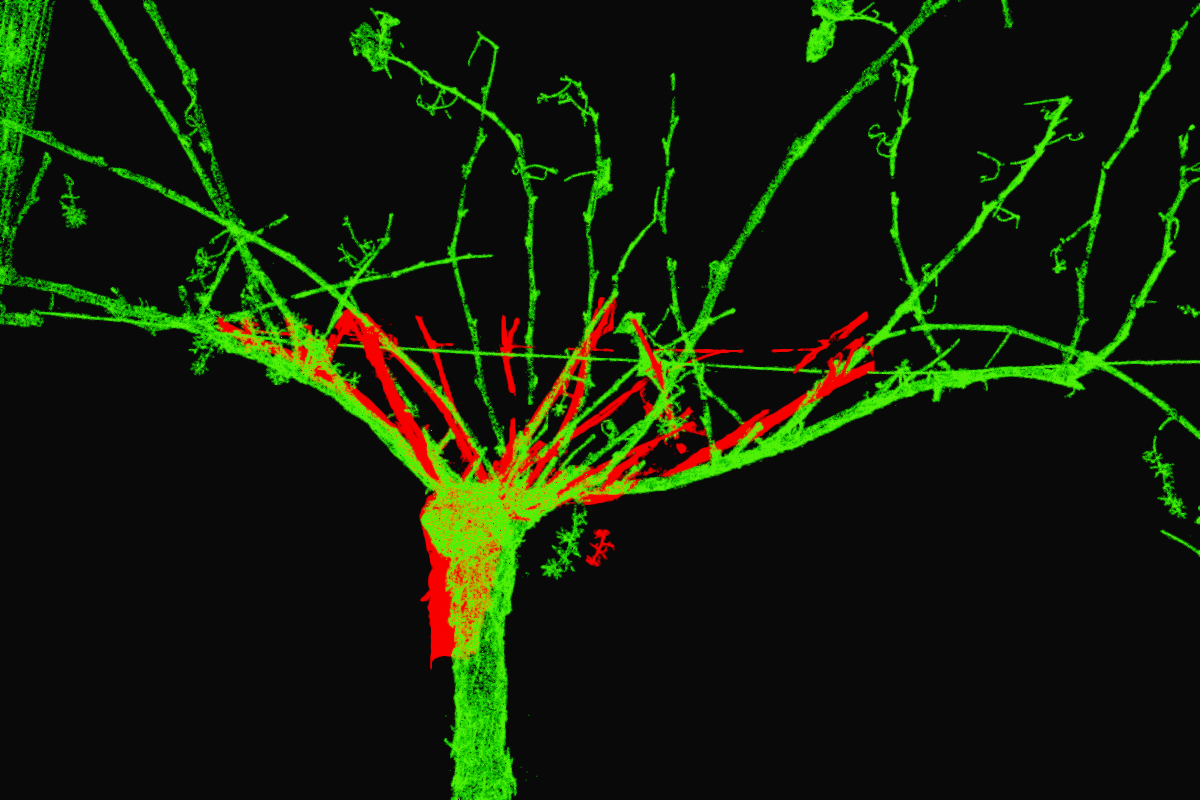
\includegraphics[width=\linewidth]{4-precise-alignment/4-results/figures/stereo_D60Ap15_5b_icp_final_side}
    \caption{D60A$+$15}
  \end{subfigure}
  \hfill
  \begin{subfigure}[b]{0.32\linewidth}
    \centering
    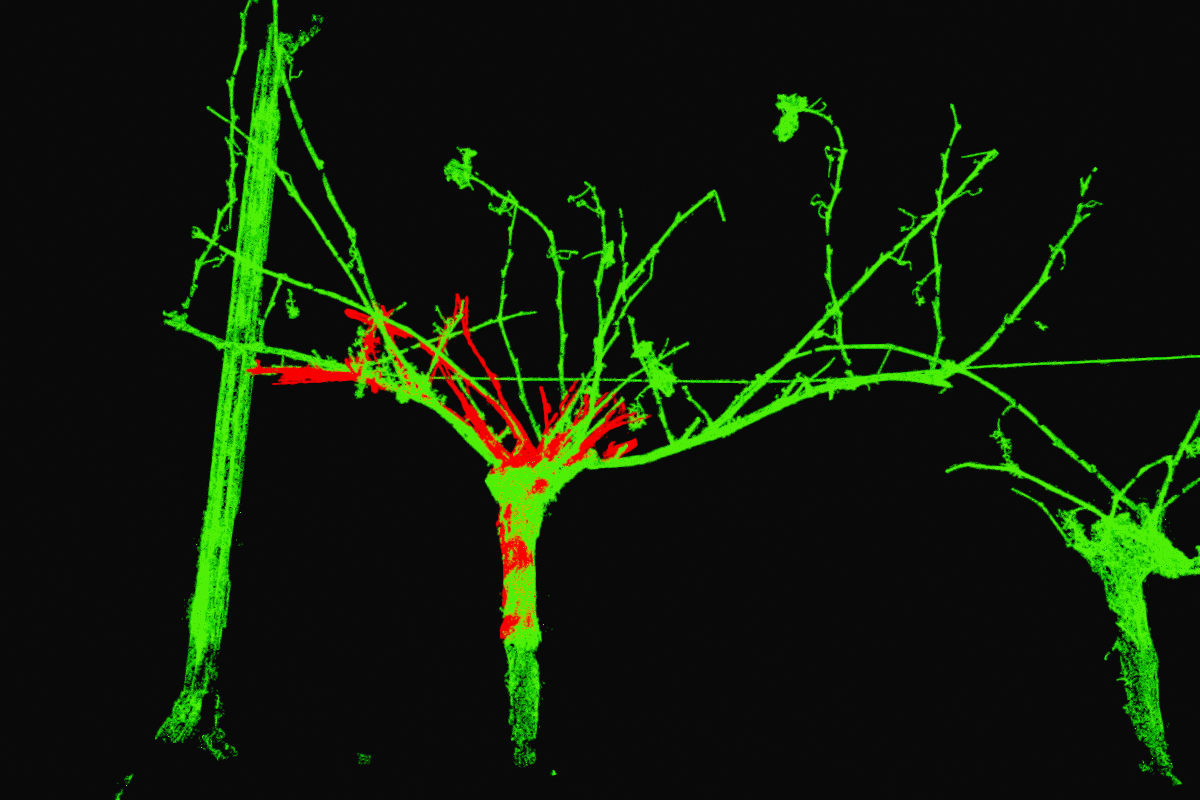
\includegraphics[width=\linewidth]{4-precise-alignment/4-results/figures/stereo_D80A0_5b_icp_final_side}
    \caption{D80A0}
  \end{subfigure}

  \vspace{0.5em}

  \begin{subfigure}[b]{0.32\linewidth}
    \centering
    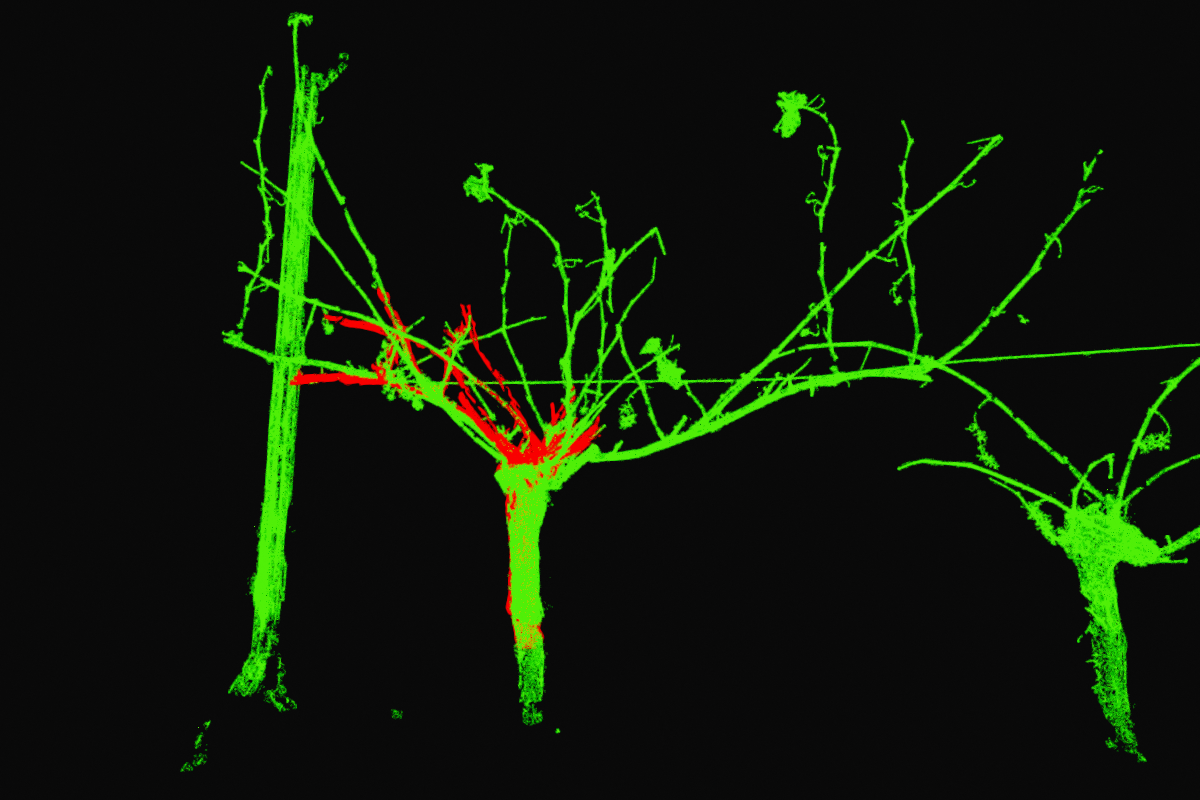
\includegraphics[width=\linewidth]{4-precise-alignment/4-results/figures/stereo_D80Ap15_5b_icp_final_side}
    \caption{D80A$+$15}
  \end{subfigure}
  \caption{Final stereo ICP alignment (vine-face view) for all seven converging conditions. Green: 3DGS reference cloud; red: registered stereo source cloud.}
  \label{fig:pa-stereo-converged-overlay}
\end{figure}

% ---------------------------------------------------------------------------
\subsection{Cross-Modal Comparison}
\label{subsec:pa-results-cross-modal}
% ---------------------------------------------------------------------------

\Cref{tab:pa-results-cross-modal} presents a matched-condition comparison of LiDAR and stereo registration outcomes. Each row corresponds to one experimental condition.

\begin{table}[htbp]
  \centering
  \small
  \setlength{\tabcolsep}{4pt}
  \caption{Matched-condition comparison of LiDAR and stereo registration outcomes. LiDAR $n_\text{acc}$: accepted hypotheses out of 35; $\tilde{\varepsilon}$: median inlier RMSE across accepted hypotheses. Stereo $\varepsilon$: single-run inlier RMSE for converging conditions. All RMSE values in millimetres.}
  \label{tab:pa-results-cross-modal}
  \begin{tabular}{@{} l r r c r @{}}
    \toprule
    \textbf{Condition} &
    \textbf{LiDAR} \boldmath$n_\text{acc}$\textbf{/35} &
    \textbf{LiDAR} \boldmath$\tilde{\varepsilon}$ \textbf{(mm)} &
    \textbf{Stereo conv.} &
    \textbf{Stereo} \boldmath$\varepsilon$ \textbf{(mm)} \\
    \midrule
    D40A$-$15 & 35/35 & 32.31 & Yes & 16.77 \\
    D40A0     & 34/35 & 35.22 & Yes & 16.77 \\
    D40A$+$15 & 35/35 & 34.85 & No  &  ---  \\
    D60A$-$15 & 35/35 & 34.94 & Yes & 16.67 \\
    D60A0     & 35/35 & 33.25 & Yes & 16.76 \\
    D60A$+$15 & 35/35 & 34.84 & Yes & 16.67 \\
    D80A$-$15 & 35/35 & 23.38 & No  &  ---  \\
    D80A0     & 32/35 & 24.41 & Yes & 12.26 \\
    D80A$+$15 & 35/35 & 23.77 & Yes & 12.64 \\
    \midrule
    \textbf{Both converged (mean)} & --- & 31.40 & --- & 15.51 \\
    \bottomrule
  \end{tabular}
\end{table}

LiDAR achieved convergence ($\geq 1$ accepted hypothesis) in all 9 conditions (100\%); stereo converged in 7 of 9 (78\%). On the seven conditions where both pipelines converged, the mean stereo RMSE is 15.51\,mm versus 31.40\,mm for LiDAR. LiDAR converged in two conditions where stereo failed (D40A$+$15 and D80A$-$15); no condition that failed for LiDAR succeeded for stereo. The mean stereo pipeline latency across all conditions is $14.18 \pm 2.59$\,s, compared to $46.0 \pm 3.8$\,s for LiDAR (excluding the 25\,s accumulation interval).


% ===========================================================================
\section{Discussion}
\label{sec:precise-alignment-discussion}
% ===========================================================================

This section interprets the quantitative results presented in \cref{sec:precise-alignment-results}, examining convergence behaviour, the effects of experimental variables (distance, angle), and the comparative strengths and limitations of the LiDAR and stereo modalities. The cross-modal trade-offs are synthesised in \cref{subsec:pa-discussion-cross-modal}.

A methodological caveat applies throughout this discussion. The fitness score and inlier RMSE reported in \cref{sec:precise-alignment-results} are \emph{internal} registration metrics: they measure geometric agreement between the source and target point clouds after alignment, not absolute pose accuracy relative to a ground-truth reference. A high fitness score is necessary but not sufficient for correct alignment; interpretations of RMSE as ``precision'' should be understood in this restricted sense. The absence of external ground truth is discussed further in \cref{subsec:pa-discussion-limitations}.

% ---------------------------------------------------------------------------
\subsection{Convergence Reliability}
\label{subsec:pa-discussion-convergence}
% ---------------------------------------------------------------------------

A pipeline that achieves low RMSE on converging trials but fails silently on a substantial fraction of conditions offers limited operational utility. In this regard, the LiDAR modality shows a clear advantage: all nine conditions converged, with 311 of 315 hypotheses accepted (98.7\% hypothesis-level acceptance). The stereo pipeline converged in seven of nine conditions (78\%).

The unperturbed initial hypothesis (Orig group) converged in all 9 conditions, with a per-hypothesis acceptance rate of 100\%, consistent with the perturbed groups (97--100\%; \cref{tab:pa-results-groups}). Furthermore, when perturbation hypotheses do converge, they reach effectively the same final pose as the initial hypothesis (\cref{tab:pa-results-lidar-sigma}). These results indicate that the perturbation strategy did not rescue any condition that would otherwise have failed; the LiDAR pipeline's convergence advantage over stereo is attributable primarily to the properties of the LiDAR-derived cost surface rather than to the multi-hypothesis architecture.

Two properties of active LiDAR sensing contribute to this well-conditioned cost surface. First, as an active sensor emitting at 905\,nm, the Livox Mid-360 LiDAR generates returns independently of ambient illumination and surface texture, producing consistent point density across conditions. Second, the near-zero within-trial pose standard deviation observed across most conditions (\cref{tab:pa-results-lidar-sigma}) suggests that the GICP cost surface contains a dominant basin sufficiently wide that all 35 perturbation hypotheses fall within it whenever the preprocessing stage produces a well-formed source cloud.

The two stereo-only failures reveal different vulnerability modes. D40A$+$15 produced 87\,994 processed points, a count comparable to the successfully converging D40A$-$15 (87\,772 points) and D40A0 (83\,163 points), yet achieved $F = 0.0$. Importantly, LiDAR's unperturbed initial hypothesis also converged on this condition, demonstrating that the failure is specific to the stereo-derived cost surface rather than an initialisation problem that perturbations could resolve. The stereo pipeline's dependence on photometric contrast for disparity estimation, combined with the geometric configuration at close range and oblique angle, likely produces a cost surface with a narrower or shallower convergence basin than the LiDAR equivalent. D80A$-$15 represents a different failure: only 23\,980 points survived preprocessing (compared to 42\,307 for D80A0 and 29\,981 for D80A$+$15), suggesting that the trunk segmentation stage was overly aggressive at this particular combination of distance and viewing angle, removing geometrically relevant structure and leaving insufficient correspondences for registration.

Although the perturbation strategy did not determine the convergence outcome in any condition tested, it provides a probabilistic safety margin against future conditions where the initial pose may fall outside the convergence basin, which is more likely in field deployment where SLAM drift is larger and vine geometry is more variable than in this controlled laboratory setting. The multi-hypothesis architecture thus functions as insurance rather than as the mechanism responsible for the observed reliability. For the stereo pipeline, the convergence gap is primarily a sensing and cost-surface conditioning problem: introducing perturbations would address the narrow-basin vulnerability demonstrated by D40A$+$15, but would not resolve failures attributable to insufficient point density (D80A$-$15). Improving stereo preprocessing robustness, particularly the trunk segmentation and depth filtering stages, would yield more direct reliability gains than adding perturbation hypotheses.

% ---------------------------------------------------------------------------
\subsection{Distance Effects on Registration Quality}
\label{subsec:pa-discussion-distance}
% ---------------------------------------------------------------------------

A counter-intuitive finding emerges from the distance analysis: the D80 group (80\,cm) achieves the lowest median inlier RMSE for both modalities (23.77\,mm for LiDAR and 12.45\,mm for stereo), outperforming both the closer D40 group (34.66\,mm LiDAR, 16.77\,mm stereo) and the D60 group (34.29\,mm LiDAR, 16.67\,mm stereo). An intuitive expectation is that closer sensing yields higher precision due to higher point density on the target structure; however, the data consistently indicate that moderate distance produces superior registration quality.

For the LiDAR modality, the geometric explanation centres on the spatial extent of structure captured within the sensor's field of view and the resulting constraint on rotational degrees of freedom. At 40\,cm, the Livox Mid-360's field of view captures only a compact segment of the vine structure: a short length of trunk and its immediate lateral canes. Although this close-range cloud is not geometrically featureless, its limited spatial extent provides a short effective lever arm for constraining rotation. A small angular misalignment applied to a spatially compact cloud produces only small positional residuals at the cloud's edges, leaving the ICP cost surface relatively flat in rotational directions and permitting the solver to terminate with residual angular error that elevates RMSE. At 80\,cm, the wider field of view encompasses a substantially larger scene: multiple vine structures, trellis posts, and guide wires in addition to the target vine's branching geometry. This extended spatial baseline means that the same rotational error produces proportionally larger residuals at distant points, sharpening the cost surface and constraining the solver to a tighter minimum. The effect is analogous to increasing baseline length in triangulation: longer baselines yield better angular resolution. The IQR data support this interpretation: D80 conditions exhibit near-zero IQR in both fitness and RMSE (\cref{tab:pa-results-lidar-per-condition}), indicating that the solver converges to a single well-defined minimum, whereas D40 conditions show slightly elevated IQR values consistent with residual rotational ambiguity from the shorter spatial baseline.

The stereo modality exhibits the same distance-RMSE trend (D80 $<$ D60 $<$ D40), though the absolute RMSE values are approximately half those of LiDAR across all distance groups. The stereo pipeline applies a near-field depth clipping threshold ($z_\text{far} = 1.0$\,m), retaining only high-confidence depth estimates within the stereo baseline's optimal operating range. At D80, this clipping window captures the vine structure at a distance where the stereo disparity estimation is geometrically well-conditioned: the baseline-to-depth ratio yields sub-pixel disparity that translates to millimetre-level depth precision, consistent with the quadratic depth-error relationship for triangulation-based systems~\cite{hartleyMultipleViewGeometry2004}. At D40, the same clipping window may include points at the extreme edges of the depth range where stereo triangulation uncertainty increases, and the very close range may introduce depth-edge artefacts from the narrow stereo baseline. The net effect is a modest but consistent RMSE advantage for the D80 group.

The practical recommendation emerging from these results is an optimal operating range of 60--80\,cm for both modalities. Within this range, convergence is reliable ($\geq 97\%$ for LiDAR, 67--100\% for stereo) and RMSE is minimised. The results also indicate that registration degrades gracefully as distance decreases below 80\,cm (higher RMSE but maintained convergence), suggesting that approaching closer than the optimal distance produces suboptimal but usable alignments. For context, prior work on LiDAR-based vine reconstruction by \citet{morenoOnGroundVineyardReconstruction2020} used a mobile mapping platform with the sensor positioned at approximately 1\,m from the crop row, though direct RMSE comparison is complicated by differences in registration targets (full canopy vs.\ isolated trunk). The sub-25\,mm LiDAR RMSE and sub-13\,mm stereo RMSE achieved at D80 place registration precision within the same order of magnitude as the target structures (5--15\,mm cane diameter), satisfying the centimetre-level accuracy goal stated in \cref{sec:research-objectives}.

% ---------------------------------------------------------------------------
\subsection{Approach Angle Effects}
\label{subsec:pa-discussion-angle}
% ---------------------------------------------------------------------------

The experimental design tested three approach angles ($-15^{\circ}$, $0^{\circ}$, $+15^{\circ}$) to assess whether oblique sensor-to-vine geometry degrades registration performance. For the LiDAR modality, the answer is negative within the tested range: both the A$-$15 and A$+$15 groups achieve 100\% hypothesis acceptance, with RMSE values (34.66\,mm and 34.28\,mm respectively) indistinguishable from the A0 group (33.25\,mm). The A0 group achieves 96\% acceptance (101/105 hypotheses), with the slight reduction attributable to D80A0 (32/35). The LiDAR pipeline is thus effectively invariant to $\pm 15^{\circ}$ approach angle variation, which is an important property for operational robustness given that a mobile platform navigating between vine rows cannot guarantee a perfectly perpendicular approach.

The stereo modality shows convergence rates of 67\% for A$-$15 and A$+$15, and 100\% for A0. D40A$+$15 failed while D40A$-$15 succeeded under nominally symmetric angular conditions. This asymmetry suggests an interaction between approach angle and the specific vine geometry at close range: a $+15^{\circ}$ approach from 40\,cm may position the cameras such that the trunk is partially occluded by a lateral cane or the initial pose estimate is offset into a region where ICP diverges.

The $\pm 15^{\circ}$ range tested here was chosen to represent a conservative estimate of lateral (yaw) approach angle variation for a mobile manipulator operating in vineyard rows. In practice, imprecise stopping (slightly early or late along the row) introduces a yaw offset between the sensor boresight and the vine centre. The stereo pipeline's relatively low convergence on angled approaches limits its viability as a standalone alignment modality; whereas the LiDAR pipeline's invariance demonstrates a more operationally robust modality.

Two additional limitations constrain the generality of the angular analysis. First, only lateral (yaw) deviations were tested. Vineyard terrain is frequently uneven, causing the robot chassis to pitch or roll relative to the vine. Vertical angular deviations could alter the point cloud overlap with the reference model in ways not captured by the lateral-only design. Second, even where the alignment pipeline tolerates $\pm 15^{\circ}$ approach angles, this does not imply that the downstream pruning operation is viable at such offsets. The robotic manipulator's reachability, joint limits, and tool-vine geometry impose additional constraints on acceptable approach angles that were not evaluated in this work. Characterising the manipulator's angular tolerance and its interaction with alignment accuracy would require integrated system-level testing beyond the scope of this evaluation.

% ---------------------------------------------------------------------------
\subsection{Perturbation Strategy Effectiveness}
\label{subsec:pa-discussion-perturbation}
% ---------------------------------------------------------------------------

The multi-hypothesis perturbation strategy generates 35 initial pose hypotheses per trial, distributed across five groups (Orig, A--E) that sample translational and rotational offsets around the SLAM-provided initial pose. Two lines of evidence indicate that these hypotheses all fall within a single dominant convergence basin. First, per-group acceptance rates are uniformly high---97\% (Group~C) to 100\% (Orig, A, B)---with median fitness and RMSE values statistically indistinguishable across groups (\cref{tab:pa-results-groups}). If local minima existed within the perturbation neighbourhood, some hypotheses would become trapped, producing disparity in convergence rates; this is not observed. Second, the within-trial convergence analysis (\cref{tab:pa-results-lidar-sigma}) shows that accepted hypotheses converge to effectively the same final pose: D80A0 achieves near-zero standard deviation across all transformation components ($\sigma < 0.1$\,mm translation, $< 0.01^{\circ}$ rotation), and D40A0, D60A$-$15, and D60A0 show similarly tight clustering. The Orig (unperturbed) group converged in every condition where any hypothesis converged (9/9), confirming that the SLAM-provided initial pose already falls within the basin.

The perturbation strategy therefore provides \emph{redundancy} rather than \emph{diversity}: its value in these experiments was not in rescuing convergence but in providing a probabilistic safety margin for future conditions where the nominal pose may fall outside the basin. With per-hypothesis convergence probability $p$, 35 independent hypotheses achieve trial-level convergence probability $1 - (1-p)^{35}$, which exceeds 99\% for any $p > 13\%$. In the present evaluation, this margin was never exercised.

The exceptions to single-basin convergence are informative. D80A$-$15 and D80A$+$15 exhibit elevated roll standard deviation ($\sigma_\phi > 6^{\circ}$), and D40A$-$15 and D40A$+$15 show moderate roll variability ($\sigma_\phi \approx 4^{\circ}$). These conditions are exclusively the angled approaches, and two factors likely contribute to the elevated roll variability. First, oblique viewing angles reduce the geometric constraint available to the ICP solver in the roll direction: when the sensor views the vine off-axis, fewer surface normals are oriented to penalise roll misalignment, producing a flatter cost surface in that degree of freedom. Second, the manually-measured initial poses for angled conditions carry higher angular uncertainty than the straight-on approaches, because positioning the robot at a precise $15^{\circ}$ offset is inherently more difficult to measure than a perpendicular alignment. This larger initial angular spread, combined with the weaker roll constraint, causes hypotheses to settle at slightly different roll values rather than converging to a single sharp minimum. The roll variability does not affect the translational components ($\sigma_{t_x}$, $\sigma_{t_y}$, $\sigma_{t_z}$ remain low for these conditions), confirming that the positional alignment is well-determined even when the rotational alignment around the trunk axis is less precisely constrained.

For operational deployment, the redundancy interpretation suggests that the number of hypotheses could be substantially reduced without sacrificing reliability. If 35 hypotheses converge to the same solution in 8 of 9 conditions, then 7--10 hypotheses would provide equivalent coverage with a threefold to fivefold reduction in computation time. The primary exception is D80A0, where only 32 of 35 hypotheses were accepted; it still shows a 91\% per-hypothesis acceptance rate, for which 10 hypotheses would yield $>$99.99\% trial-level convergence probability. Such a reduction would bring the LiDAR pipeline's timing from $\sim$46\,s down to $\sim$12--15\,s, approaching the stereo pipeline's latency and substantially improving real-time feasibility without requiring algorithmic parallelisation.

% ---------------------------------------------------------------------------
\subsection{Cross-Modal Trade-offs}
\label{subsec:pa-discussion-cross-modal}
% ---------------------------------------------------------------------------

The matched-condition comparison (\cref{tab:pa-results-cross-modal}) summarises the central finding of this evaluation: the LiDAR and stereo modalities occupy complementary positions in the reliability--precision--speed trade-off space. Neither modality dominates the other across all axes of performance, and the choice between them (or the strategy for combining them) depends on the priorities of the downstream operations.

On the seven conditions where both pipelines converged, stereo achieves a mean inlier RMSE of 15.51\,mm compared to 31.40\,mm for LiDAR, a factor-of-two precision advantage. This difference is not primarily attributable to the ICP algorithm (both pipelines use the same GICP solver with identical convergence parameters) but to the quality of the input point clouds. At close range, stereo imaging produces denser and more spatially uniform point clouds than mechanical LiDAR, which remains comparatively sparse even after prolonged scan accumulation~\cite{stenEnhancingOffRoadTopography2025}. The stereo pipeline yields a compact, high-fidelity cloud of 68\,k--92\,k points from a single frame pair, with near-uniform surface sampling concentrated on the vine structure. The LiDAR pipeline accumulates 97\,k--133\,k points over 25\,s, yet these are distributed across a wider spatial extent with less uniform surface coverage. The higher point density and surface completeness of the stereo cloud provides GICP with a more tightly constrained correspondence set, contributing to the observed increased precision. RMSE as reported here measures the \emph{internal consistency} of inlier correspondences; the mean distance between matched source-target point pairs after alignment, rather than absolute positional accuracy relative to a ground-truth pose. A low RMSE indicates tight geometric agreement between the registered clouds, which is a close proxy condition for pose accuracy but not a comprehensive one.

The reliability advantage of LiDAR is clear: 100\% condition-level convergence versus 78\% for stereo. LiDAR converged in two conditions where stereo failed (D40A$+$15 and D80A$-$15), while no condition that failed for LiDAR succeeded for stereo. As discussed in \cref{subsec:pa-discussion-convergence}, this asymmetry is primarily attributable to the properties of active sensing (illumination independence, consistent point density, and the resulting well-conditioned cost surface) rather than to the multi-hypothesis architecture, which provided redundancy but did not rescue any condition that the unperturbed initial hypothesis would have failed. Stereo, as a passive modality, depends on photometric contrast for disparity estimation; in a laboratory environment this is not limiting, but in field conditions where lighting varies and surfaces may be wet or uniformly coloured, the reliability gap could widen further. The result that LiDAR succeeds everywhere stereo succeeds (but not vice versa) suggests that stereo failures are sensing or preprocessing problems rather than fundamental geometric insufficiency.

The timing differential is substantial. The stereo pipeline completes in $14.18 \pm 2.59$\,s with no preceding accumulation interval, whereas the LiDAR pipeline requires $46.0 \pm 3.8$\,s of processing plus a 25\,s scan accumulation phase (though accumulation can overlap with prior-vine pruning). In pruning systems where the total per-vine cycle is on the order of 100--120\,s~\cite{botterillRobotSystemPruning2017, hizatateDevelopmentRobotPruning2025}, the stereo pipeline's 14\,s alignment latency represents a minor fraction of cycle time, whereas the LiDAR pipeline's 71\,s combined accumulation and processing time becomes the dominant contributor to cycle duration. However, as discussed in \cref{subsec:pa-discussion-perturbation}, reducing the hypothesis count from 35 to 7--10 would bring LiDAR processing from $\sim$46\,s down to $\sim$12--15\,s, yielding a combined latency of $\sim$37--40\,s (including the 25\,s scan accumulation) that is more readily accommodated within the pruning cycle.

The cross-modal comparison also validates the two-stage localisation architecture proposed in this thesis. The ICP corrections reported in \cref{tab:pa-results-lidar-icp-correction,tab:pa-results-stereo-transforms} range from 46.6\,mm to 165.3\,mm in translational displacement and from $0.13^{\circ}$ to $11.5^{\circ}$ in rotational correction. These magnitudes are consistent with the SLAM system's (GLIM-GNSS) absolute trajectory error of 71--174\,mm reported in \cref{chap:SLAM}, confirming that the coarse localisation delivered by SLAM places the robot within ICP's convergence basin. The perturbation strategy samples $\pm 50$\,mm translation and $\pm 15^{\circ}$ rotation around the SLAM pose, and achieves 98.7\% hypothesis-level convergence, which is evidence that the SLAM accuracy is sufficient for the precise-alignment stage to function reliably. The two-stage architecture thus combines capabilities that neither stage provides independently: SLAM provides global consistency and centimetre-level initial pose, while ICP refines this to millimetre-level alignment against the reference model.

% ---------------------------------------------------------------------------
\subsection{Pipeline Timing and Real-Time Feasibility}
\label{subsec:pa-discussion-timing}
% ---------------------------------------------------------------------------

The concept of ``real-time'' in the context of robotic vine pruning is defined not by absolute latency thresholds but by alignment latency as a proportion of the total per-vine cycle. Published pruning systems report per-vine cycle times of approximately 120\,s~\cite{botterillRobotSystemPruning2017} and 107\,s~\cite{hizatateDevelopmentRobotPruning2025}, encompassing perception, planning, and manipulator execution. Alignment is necessarily sequential---motion planning cannot begin until the aligned pose is available---so its latency adds directly to cycle time. Under this framing, an alignment latency of 10--15\,s ($\sim$10--14\% of the per-vine cycle) has minimal impact on throughput, whereas latency exceeding 60\,s would increase cycle time by more than 50\% and become the dominant bottleneck.

The stereo pipeline, with a mean total latency of $14.18 \pm 2.59$\,s, already satisfies this real-time criterion. Its timing decomposition (\cref{tab:pa-results-stereo-timing}) reveals that the dominant components are ICP alignment ($7.41 \pm 2.56$\,s) and dual-camera combination ($4.60 \pm 0.16$\,s), with GPU-accelerated depth estimation via FoundationStereo contributing only 1.2\,s. The combination stage ($4.60 \pm 0.16$\,s) is largely a synchronisation cost: each camera's depth estimation and filtering must complete sequentially before the trivial point cloud merge can proceed. Since the GPU-accelerated stereo inference serialises access to the GPU, the two cameras cannot be processed fully in parallel without additional hardware resources. The ICP latency is determined by cloud size and convergence speed, both of which are already favourable for the stereo pipeline's relatively compact clouds (68\,000--92\,000 processed points). No architectural changes are required for the stereo pipeline to operate within the pruning cycle's time budget.

The LiDAR pipeline's current latency of $46.0 \pm 3.8$\,s (\cref{tab:pa-results-lidar-timing}), plus 25\,s scan accumulation, substantially exceeds the real-time threshold. However, the timing structure illustrates that the majority of the latency is from the sequential execution of ICP, rather than a fundamental computational limit. These hypotheses are \emph{embarrassingly parallel}: they share the same source and target clouds, differ only in their initial transformation, and produce independent results. Since the hypotheses require no inter-process communication, concurrent execution on parallel hardware would reduce the registration phase from $\sim$34\,s to the cost of a single hypothesis ($\sim$1\,s). Combined with the 0.71\,s preprocessing overhead, the parallelised ICP LiDAR pipeline would achieve $\sim$2\,s active computation time, which would be faster than the stereo pipeline. The 25\,s accumulation interval can be overlapped with the preceding vine's pruning execution, effectively removing it from the critical path. With parallelisation and accumulation overlap, the LiDAR pipeline's effective per-vine latency would approach 2--3\,s, well within real-time constraints. the hypothesis reduction discussed in \cref{subsec:pa-discussion-perturbation} (from 35 to 7--10 hypotheses) would achieve a similar latency improvement ($\sim$10--12\,s) without requiring parallel hardware, representing a path to real-time operation that requires minimal engineering effort.

% ---------------------------------------------------------------------------
\subsection{Limitations}
\label{subsec:pa-discussion-limitations}
% ---------------------------------------------------------------------------

The most significant limitation of this evaluation is the absence of an external six-degree-of-freedom ground-truth measurement. All reported metrics (fitness score and inlier RMSE) are \emph{internal consistency} measures: they quantify how well the source and target point clouds agree geometrically after registration, but cannot determine whether the recovered pose is correct in an absolute sense. A registration that achieves high fitness and low RMSE could, in principle, converge to a self-consistent but incorrect local minimum, particularly if both clouds share systematic biases (e.g., both derived from the same sensor platform with an uncalibrated extrinsic offset). The visual alignment overlays (\cref{fig:pa-lidar-alignment-examples,fig:pa-stereo-converged-overlay}) provide qualitative evidence that the registrations are geometrically plausible, but qualitative assessment cannot substitute for quantitative validation against an independent pose reference such as a motion capture system or precision-surveyed fiducial markers. Future work should incorporate such ground truth to establish absolute pose accuracy bounds and determine whether the RMSE values reported here correspond to comparable levels of absolute error.

The evaluation was conducted on two dormant vine specimens in a controlled laboratory environment. While this approach eliminates confounding factors and permits precise control of experimental variables, it leaves open the question of generalisation. Field conditions introduce multiple sources of variability absent from the laboratory: wind-induced motion of canes and foliage (particularly relevant for non-dormant canopy), varying vine structure across cultivars, training systems, and ages, canopy interference from adjacent rows, variable ambient lighting affecting stereo depth estimation, and surface contamination (mud, water droplets) affecting LiDAR reflectance. Each of these factors could independently degrade registration performance, and their combined effect in field conditions is unknown. 

Conversely, the laboratory environment under-represents the geometric information available to the LiDAR pipeline in a vineyard setting. In these experiments, the accumulated LiDAR cloud was cropped to a narrow angular aperture containing only the immediate test vine, because the surrounding laboratory environment is not representative of the operational environment. In a vineyard row, the full 360° LiDAR scan would capture multiple adjacent vines simultaneously, each of which could be registered against its corresponding reference model. Aligning against several spatially distributed reference structures would provide substantially more geometric constraint than a single-vine registration, likely improving both convergence reliability and pose precision for the LiDAR modality. The single-vine, narrow-aperture evaluation presented here therefore represents a conservative assessment of LiDAR alignment performance relative to field deployment.

The experimental design employs a $3 \times 3$ factorial with a single observation per condition ($n = 1$). This design is sufficient to characterise broad performance trends (distance effects, modality differences) but insufficient for rigorous statistical inference. Without replicates, it is impossible to distinguish genuine condition effects from trial-specific noise. For example, the D40A$+$15 stereo failure could reflect a systematic vulnerability at that condition or a stochastic event that would not recur on a second trial. The absence of repeated measurements also precludes assessment of measurement repeatability: that is, the extent to which the same condition produces the same alignment result across multiple independent trials. For a pruning system that must reliably position a cutting tool within millimetres of a target, repeatability is as important as accuracy for operational deployment, and this evaluation provides no information on that axis.

The condition-specific stereo failures (D40A$+$15 and D80A$-$15) may be partially specific to the test vine's geometry and the chosen preprocessing parameters. The D40A$+$15 stereo failure may reflect a geometric interaction between the particular arrangement of canes on this vine and the camera viewpoint at that condition, rather than a general vulnerability of the stereo pipeline at 40\,cm with $+15^{\circ}$ approach angle. Similarly, the D80A$-$15 failure appears linked to overly aggressive trunk segmentation at that viewing angle. Characterising the robustness of these failure boundaries would require testing across multiple vine specimens in several different vineyards, which is left as future work.

Finally, the preprocessing pipeline represents a confounding factor in attributing performance characteristics to the sensing modality versus the algorithmic choices. Failures attributed to ``the LiDAR pipeline'' conflate the Livox Mid-360's sensing capabilities with the specific Patchwork++ parameterisation, the statistical outlier rejection thresholds, and the voxel downsampling resolution; similarly, ``stereo pipeline'' failures conflate FoundationStereo's depth estimation with the DBSCAN clustering parameters, morphological closing kernel size, and the $z_\text{far}$ clipping threshold. A different parameterisation of these preprocessing stages might shift the convergence boundaries or alter the RMSE characteristics. Disentangling the contributions of sensing physics from algorithmic preprocessing choices would require ablation studies that systematically vary preprocessing parameters while holding the sensing modality constant, an analysis beyond the scope of this evaluation but necessary for informed pipeline optimisation in future deployments.


\section{Summary}
\label{sec:precise-alignment-summary}

This chapter presented a GICP-based point cloud registration pipeline for centimetre-scale pose refinement against a 3D Gaussian Splatting reference model, evaluated with two sensing modalities across a $3 \times 3$ factorial design of sensor-to-vine distance and approach angle. The LiDAR pipeline achieved 100\% condition-level convergence (311/315 hypotheses accepted) with a median inlier RMSE of 33.25\,mm and mean latency of 46\,s, while the stereo pipeline converged in seven of nine conditions with a mean inlier RMSE of 15.51\,mm and mean latency of 14.18\,s. Neither modality dominated: LiDAR provided superior convergence reliability attributable to its active sensing physics, whereas stereo achieved approximately half the RMSE when converging. The discussion highlighted that the multi-hypothesis perturbation strategy provided redundancy rather than diversity, that moderate operating distance (60--80\,cm) produced the best registration quality for both modalities, and that the ICP corrections fell within the SLAM system's expected error bounds, validating the two-stage localisation architecture.

\chapter{Conclusion}
\label{chap:Conclusion}

This thesis addressed the localisation requirements of autonomous vineyard pruning robots, where navigation-grade pose estimates are insufficient for millimetre-scale manipulation. A two-stage hierarchical architecture was proposed: a LiDAR-inertial SLAM system provides a coarse global pose, which is subsequently refined through point cloud registration against a pre-built 3D Gaussian Splatting reference model of the target vine.

The SLAM stage (\cref{chap:SLAM}) evaluated three configurations of increasing capability. The final GLIM-GNSS system, which augments LiDAR-inertial odometry with sparse GNSS factor injection, achieved absolute trajectory errors of 71--174\,mm across five vineyard datasets with error rates of 0.013--0.050\% per metre, satisfying the sub-decimetre accuracy target stated in \cref{sec:research-objectives}. Evaluation on a held-out dataset confirmed that this performance generalises to unseen routes with near-deterministic run-to-run consistency.

The precise-alignment stage (\cref{chap:precise-alignment}) evaluated LiDAR and stereo vision modalities for GICP registration against the 3DGS model across nine experimental conditions. The LiDAR pipeline achieved 100\% condition-level convergence with a median inlier RMSE of 33.25\,mm; the stereo pipeline converged in seven of nine conditions with a mean inlier RMSE of 15.51\,mm. The sub-centimetre accuracy target was not fully achieved by either modality, though stereo registration at 80\,cm operating distance approached it (12--13\,mm RMSE). The ICP corrections applied ranged from 47 to 165\,mm, consistent with the SLAM system's error magnitude, confirming that the coarse pose reliably places the robot within the registration algorithm's convergence basin.

The two-stage architecture was thus validated in its core design premise: neither stage alone provides what the combined system delivers. SLAM supplies global consistency and sufficient initial accuracy for ICP convergence; ICP refines this estimate to millimetre-level geometric agreement with the reference model. The system demonstrated feasibility for the vine-scale localisation problem. Under the narrow-aperture indoor conditions tested, stereo achieved the lowest RMSE within real-time latency constraints, while LiDAR provided better convergence reliability. In field deployment, where the full 360° LiDAR scan would register against a spatially extended reference model spanning multiple bays, the additional geometric constraint may narrow or eliminate the RMSE gap observed here; making this hypothesis a priority for future work.

\section{Future Work}
\label{sec:future-work}

The results presented in this thesis establish a  two-stage localisation architecture; several directions extend these capabilities toward full field deployment. The most immediate is outdoor validation of the precise-alignment stage under operational vineyard conditions. The SLAM pipeline was already evaluated on data collected in working vineyards; extending the registration pipeline to the same environment would characterise its behaviour under wind-induced vine motion, variable ambient lighting, and diverse cultivar geometries. Field trials incorporating an independent six-degree-of-freedom pose reference (e.g.\ a motion capture system or precision-surveyed fiducial markers) would establish absolute accuracy bounds, complementing the internal consistency metrics reported here.

The 100\% condition-level convergence observed for LiDAR motivates evaluation on a larger and more diverse set of vines spanning multiple vineyards, cultivars, and ages. Such testing would confirm the generality of the demonstrated low-centimetre accuracy and would provide the repeated measurements necessary to quantify run-to-run repeatability across the vine population.

A further direction is evaluating the LiDAR pipeline in vineyard conditions using the full 360° point cloud rather than the narrow angular aperture used in the indoor trials. Given that the LiDAR modality already achieves 100\% convergence with only a single-vine field of view, registering against a spatially extended 3DGS model spanning several bays and both adjacent rows would provide substantially more geometric constraint. This additional structure is expected to improve both convergence reliability and pose precision by exploiting the extended spatial baseline available in operational deployments.

On the computational side, the finding that all 35 hypothesis initialisations converge to the same solution for LiDAR registration enables a reduction to real-time operation: reducing the hypothesis count to 7--10 or parallelising the embarrassingly independent GICP runs across multiple cores would reduce pipeline latency from approximately 46\,s to 10--15\,s without sacrificing the demonstrated reliability.

The stereo pipeline uses FoundationStereo~\cite{wenFoundationStereoZeroShot2025} in a zero-shot configuration without domain-specific fine-tuning. On the KITTI~2015 leaderboard, fine-tuned stereo methods achieve approximately 2$\times$ lower error rates (e.g.\ D1-all of 1.28\% for fine-tuned methods versus 2.8\% for FoundationStereo zero-shot). Domain-specific fine-tuning of FoundationStereo on vineyard imagery therefore represents a direct path to reducing the stereo depth error component of registration RMSE. The existing 3DGS vineyard model could itself serve as a source of pseudo-ground-truth training data by rendering synthetic stereo pairs with known disparity, enabling a self-supervised adaptation loop without manual annotation.

The reference model itself offers room for improvement. The 3DGS models used in these experiments were reconstructed from single-sided imagery (front face of the vine only), leaving the rear surface unrepresented. Two-sided capture, which the research group has since adopted, provides correspondences from all sensor return directions, increases the inlier count available to ICP, and would likely improve registration accuracy and robustness.

End-to-end system integration testing by coupling the SLAM-derived coarse pose with precise-alignment refinement and downstream manipulator path planning would validate that the centimetre-scale registration accuracy demonstrated here translates to successful physical pruning operations under field conditions.



\bibliography{MastersThesis}

\backmatter
\appendix
\chapter{Supplementary Figures}
\label{app:supplementary_figures}

This appendix presents additional figures that support the analysis in the main chapters but are not essential to following the primary narrative.

% ===== SLAM: Error Distribution =====
\section{SLAM Parameter Optimisation}
\label{app:slam-optimisation-figures}

\cref{fig:comparison_dist} shows the distribution of per-iteration errors across the four optimisation stages. \cref{fig:baseline_error_dist} plots the error percentage per metre for the baseline GLIM tuning, and \cref{fig:proposed_error_dist} plots the GASP metric for GLIM-GNSS tuning. Both plots use a logarithmic horizontal axis.

\begin{figure}[htbp]
     \centering
     \begin{subfigure}[b]{0.8\textwidth}
         \centering
         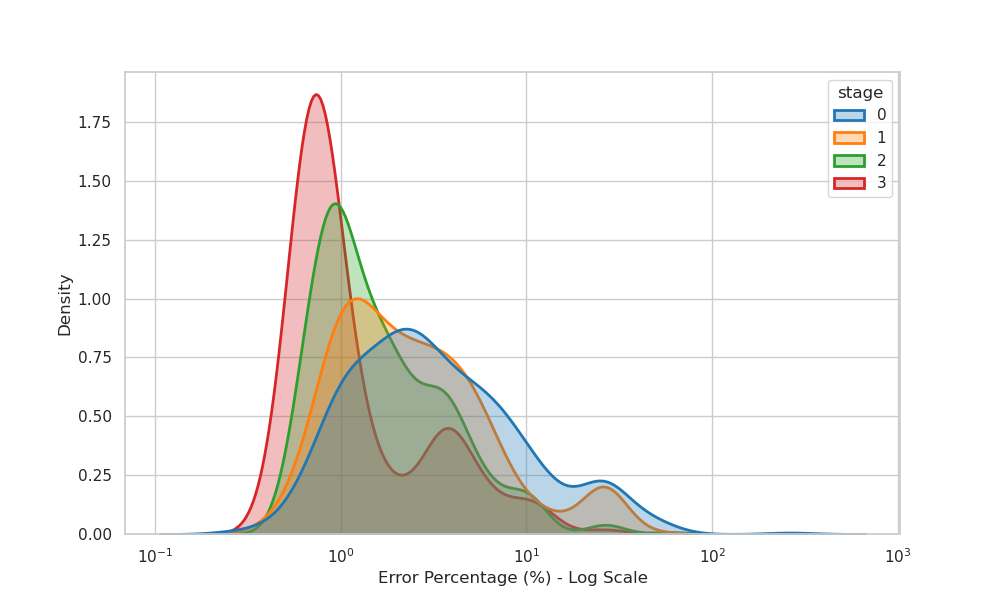
\includegraphics[width=\textwidth]{3-SLAM/3-results/figures/glim_error_distribution_by_stage_log.png}
         \caption{Baseline GLIM tuning.}
         \label{fig:baseline_error_dist}
     \end{subfigure}
     
     \vspace{1em}
     
     \begin{subfigure}[b]{0.8\textwidth}
         \centering
         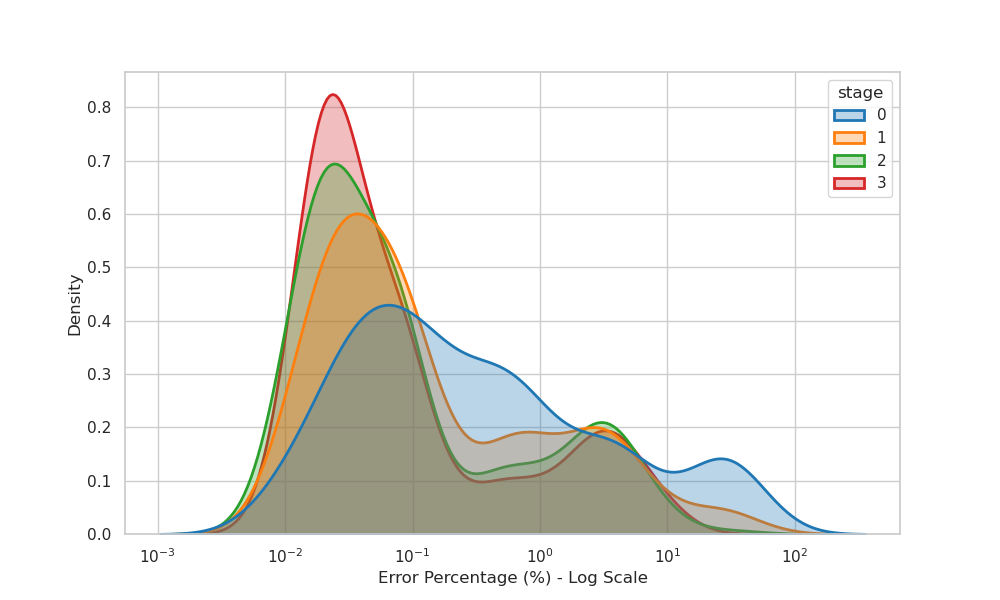
\includegraphics[width=\textwidth]{3-SLAM/3-results/figures/proposed_error_distribution_by_stage_log.png}
         \caption{GLIM-GNSS tuning.}
         \label{fig:proposed_error_dist}
     \end{subfigure}
     
     \caption{Error distribution (log scale) over optimisation stages for baseline tuning (error = error percentage) and GLIM-GNSS tuning (error = GASP).}
     \label{fig:comparison_dist}
\end{figure}

\cref{fig:comparison_progression} plots the best consensus error at the end of each optimisation stage. \cref{fig:baseline_progression} tracks the error percentage for the baseline GLIM, and \cref{fig:proposed_progression} tracks the GASP metric for GLIM-GNSS.

\begin{figure}[htbp]
     \centering
     \begin{subfigure}[b]{0.8\textwidth}
         \centering
         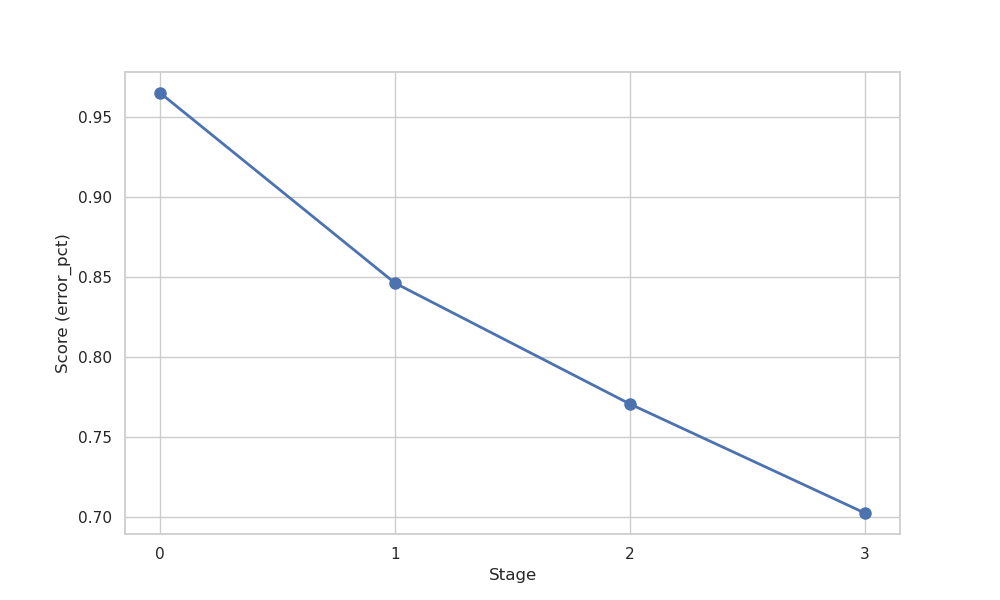
\includegraphics[width=\textwidth]{3-SLAM/3-results/figures/glim_consensus_progression.png}
         \caption{Baseline GLIM error percentage.}
         \label{fig:baseline_progression}
     \end{subfigure}

     \vspace{1.5em}

     \begin{subfigure}[b]{0.8\textwidth}
         \centering
         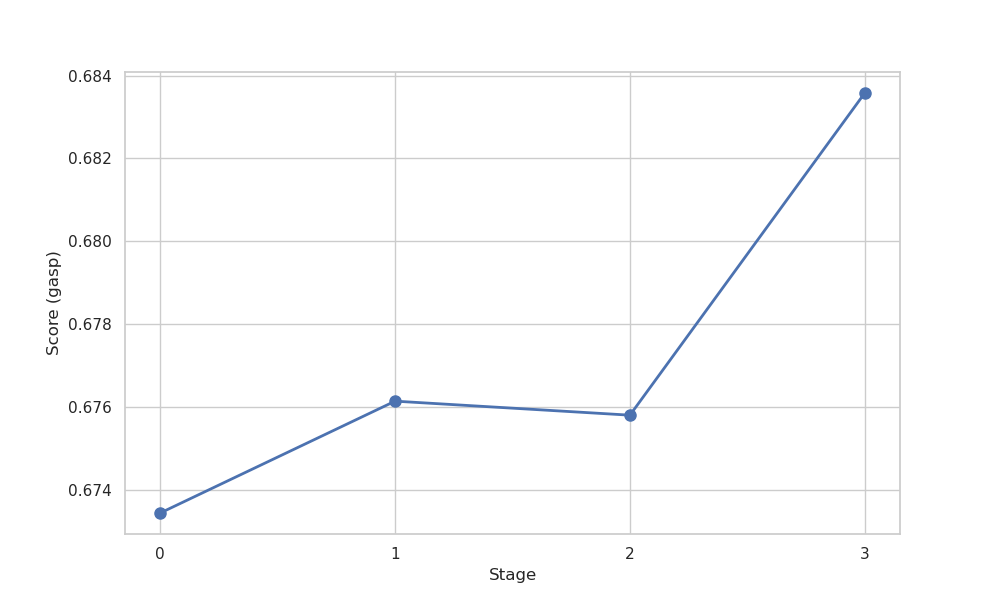
\includegraphics[width=\textwidth]{3-SLAM/3-results/figures/proposed_consensus_progression.png}
         \caption{GLIM-GNSS GASP error.}
         \label{fig:proposed_progression}
     \end{subfigure}
     
     \caption{Consensus error over optimisation stages for baseline tuning (error = error percentage) and GLIM-GNSS tuning (error = GASP).}
     \label{fig:comparison_progression}
\end{figure}

% ===== SLAM: Trajectory Grids =====
\section{SLAM Trajectory Visualisations}
\label{app:slam-trajectory-figures}

\cref{fig:large_grid_xy} presents the planar ($x$--$y$) trajectories for each dataset. The left column shows the refined GLIM output and the right column shows GLIM-GNSS output, both plotted against the RTK~GNSS ground truth.

\begin{figure}[htbp]
    \centering
    % --- ROW 1 ---
    \begin{subfigure}[b]{0.48\textwidth}
        \centering
        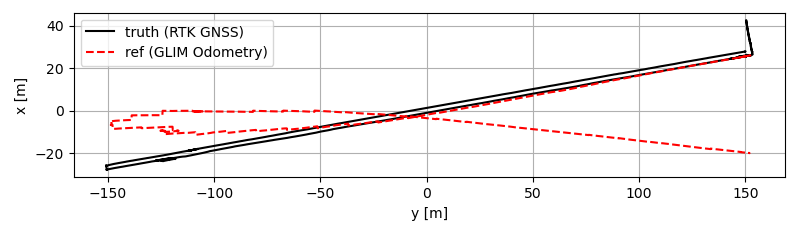
\includegraphics[width=\textwidth]{3-SLAM/3-results/figures/ds0_xy.png}
        \caption{Baseline | Dataset 0}
        \label{fig:ds0_xy_baseline}
    \end{subfigure}
    \hfill
    \begin{subfigure}[b]{0.48\textwidth}
        \centering
        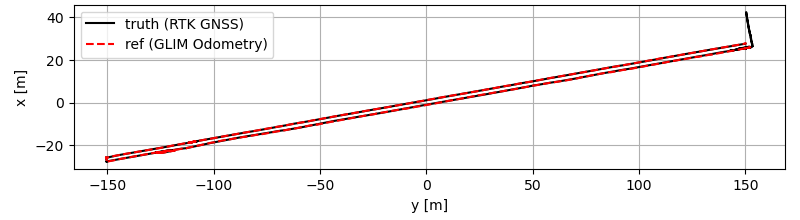
\includegraphics[width=\textwidth]{3-SLAM/3-results/figures/pds0_xy.png}
        \caption{GLIM-GNSS | Dataset 0}
    \end{subfigure}

    \vspace{1em}

    % --- ROW 2 ---
    \begin{subfigure}[b]{0.48\textwidth}
        \centering
        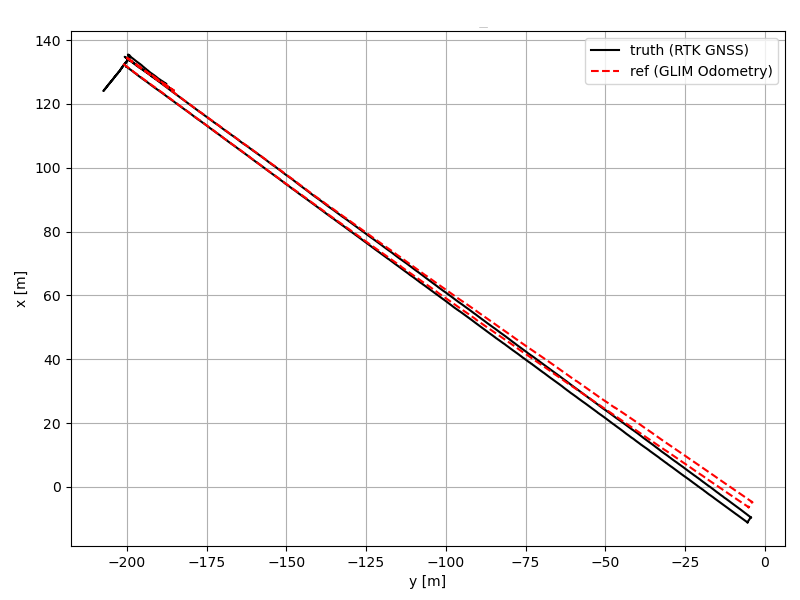
\includegraphics[width=\textwidth]{3-SLAM/3-results/figures/ds1_xy.png}
        \caption{Baseline | Dataset 1}
    \end{subfigure}
    \hfill
    \begin{subfigure}[b]{0.48\textwidth}
        \centering
        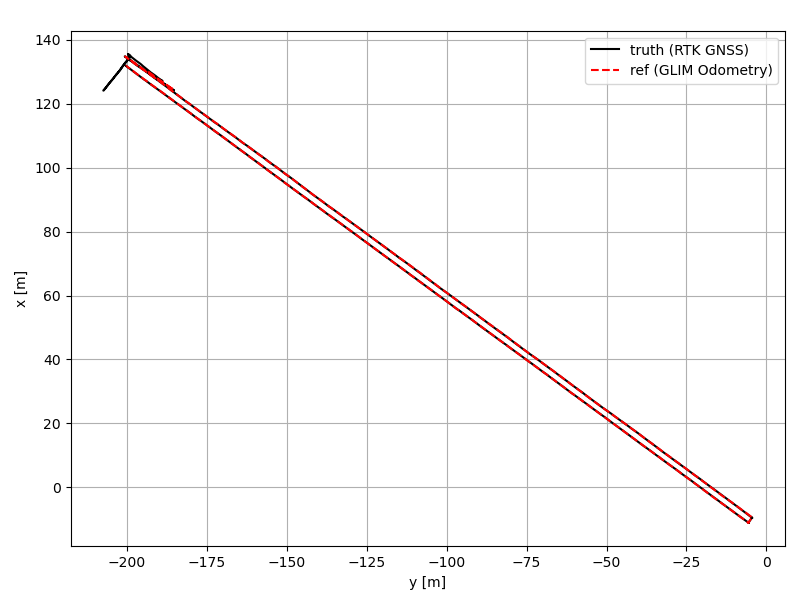
\includegraphics[width=\textwidth]{3-SLAM/3-results/figures/pds1_xy.png}
        \caption{GLIM-GNSS | Dataset 1}
    \end{subfigure}

    \vspace{1em}

    % --- ROW 3 ---
    \begin{subfigure}[b]{0.48\textwidth}
        \centering
        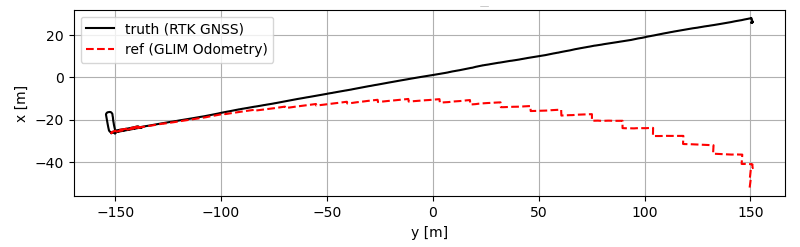
\includegraphics[width=\textwidth]{3-SLAM/3-results/figures/ds2_xy.png}
        \caption{Baseline | Dataset 2}
    \end{subfigure}
    \hfill
    \begin{subfigure}[b]{0.48\textwidth}
        \centering
        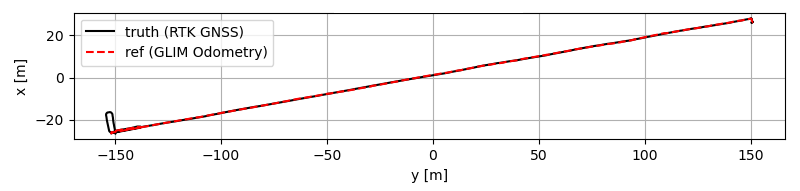
\includegraphics[width=\textwidth]{3-SLAM/3-results/figures/pds2_xy.png}
        \caption{GLIM-GNSS | Dataset 2}
    \end{subfigure}

    \vspace{1em}

    % --- ROW 4 ---
    \begin{subfigure}[b]{0.48\textwidth}
        \centering
        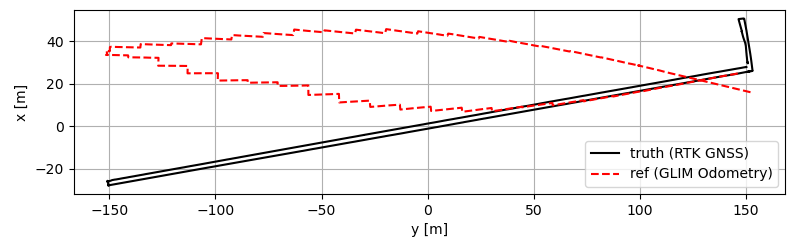
\includegraphics[width=\textwidth]{3-SLAM/3-results/figures/ds3_xy.png}
        \caption{Baseline | Dataset 3}
    \end{subfigure}
    \hfill
    \begin{subfigure}[b]{0.48\textwidth}
        \centering
        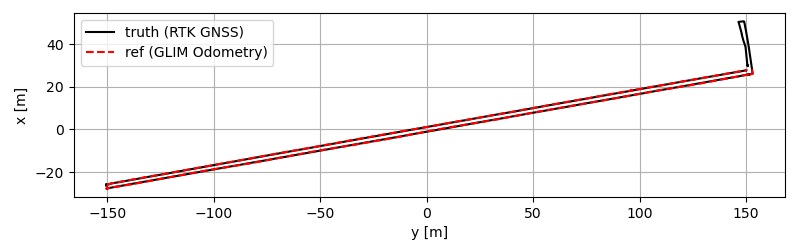
\includegraphics[width=\textwidth]{3-SLAM/3-results/figures/pds3_xy.png}
        \caption{GLIM-GNSS | Dataset 3}
    \end{subfigure}

    \vspace{1em}

    % --- ROW 5 ---
    \begin{subfigure}[b]{0.48\textwidth}
        \centering
        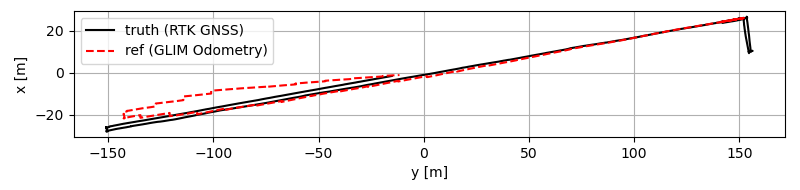
\includegraphics[width=\textwidth]{3-SLAM/3-results/figures/ds4_xy.png}
        \caption{Baseline | Dataset 4}
    \end{subfigure}
    \hfill
    \begin{subfigure}[b]{0.48\textwidth}
        \centering
        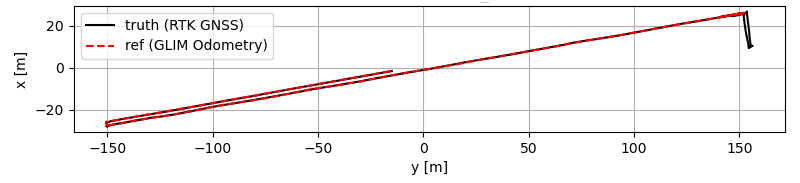
\includegraphics[width=\textwidth]{3-SLAM/3-results/figures/pds4_xy.png}
        \caption{GLIM-GNSS | Dataset 4}
    \end{subfigure}

    \caption{Trajectories in XY plane from baseline GLIM and GLIM-GNSS.}
    \label{fig:large_grid_xy}
\end{figure}

\cref{fig:large_grid_z} presents the altitude ($z$-axis) trajectories for each dataset in the same layout, with the refined GLIM estimates on the left and GLIM-GNSS estimates on the right, both compared against RTK~GNSS ground truth.

\begin{figure}[htbp]
    \centering
    % --- ROW 1 ---
    \begin{subfigure}[b]{0.48\textwidth}
        \centering
        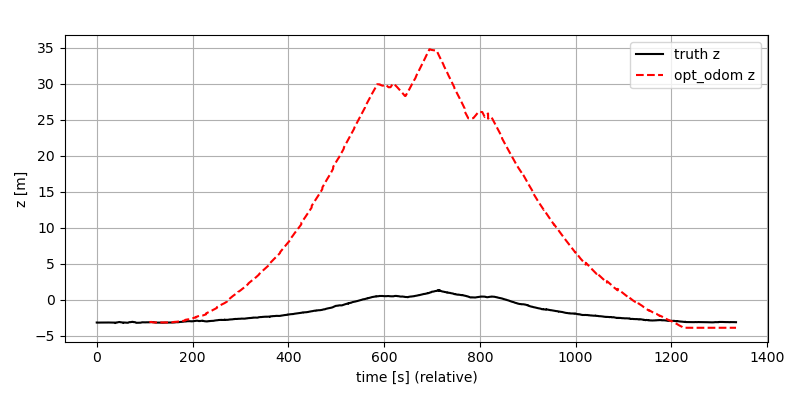
\includegraphics[width=\textwidth]{3-SLAM/3-results/figures/ds0_z.png}
        \caption{Baseline | Dataset 0}
    \end{subfigure}
    \hfill
    \begin{subfigure}[b]{0.48\textwidth}
        \centering
        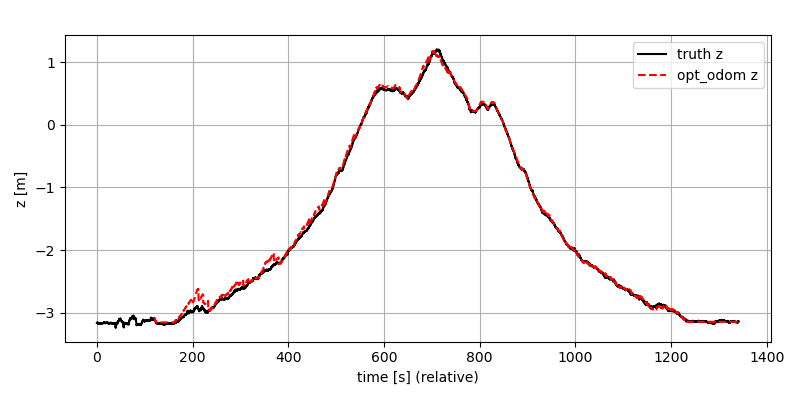
\includegraphics[width=\textwidth]{3-SLAM/3-results/figures/pds0_z.png}
        \caption{GLIM-GNSS | Dataset 0}
    \end{subfigure}

    \vspace{1em}

    % --- ROW 2 ---
    \begin{subfigure}[b]{0.48\textwidth}
        \centering
        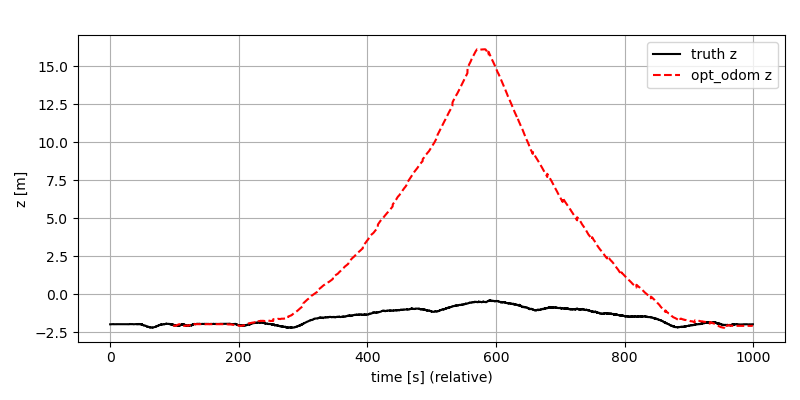
\includegraphics[width=\textwidth]{3-SLAM/3-results/figures/ds1_z.png}
        \caption{Baseline | Dataset 1}
    \end{subfigure}
    \hfill
    \begin{subfigure}[b]{0.48\textwidth}
        \centering
        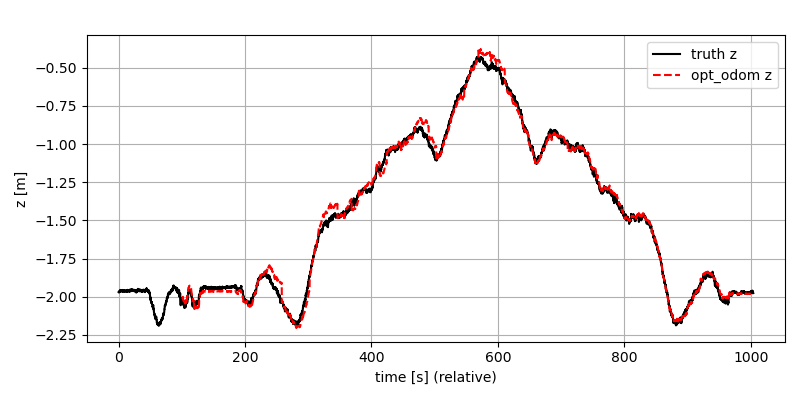
\includegraphics[width=\textwidth]{3-SLAM/3-results/figures/pds1_z.png}
        \caption{GLIM-GNSS | Dataset 1}
    \end{subfigure}

    \vspace{1em}

    % --- ROW 3 ---
    \begin{subfigure}[b]{0.48\textwidth}
        \centering
        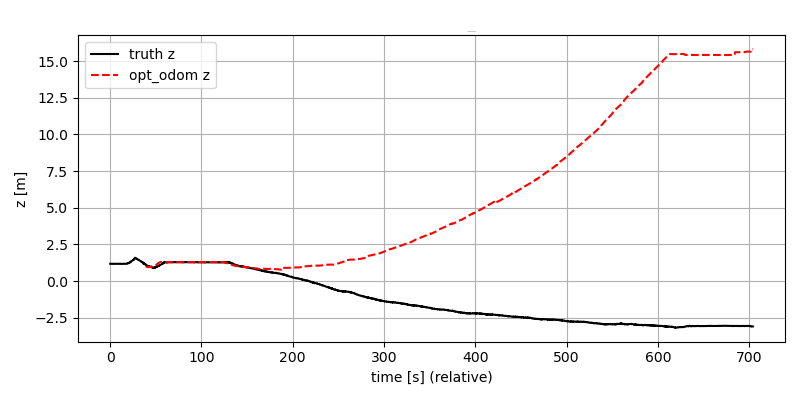
\includegraphics[width=\textwidth]{3-SLAM/3-results/figures/ds2_z.png}
        \caption{Baseline | Dataset 2}
    \end{subfigure}
    \hfill
    \begin{subfigure}[b]{0.48\textwidth}
        \centering
        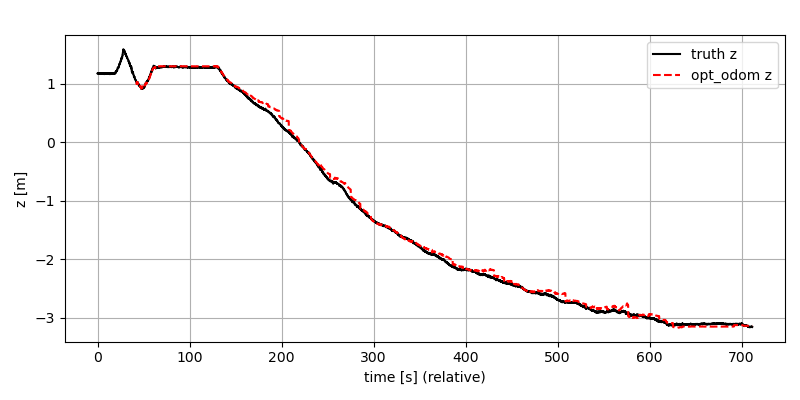
\includegraphics[width=\textwidth]{3-SLAM/3-results/figures/pds2_z.png}
        \caption{GLIM-GNSS | Dataset 2}
    \end{subfigure}

    \vspace{1em}

    % --- ROW 4 ---
    \begin{subfigure}[b]{0.48\textwidth}
        \centering
        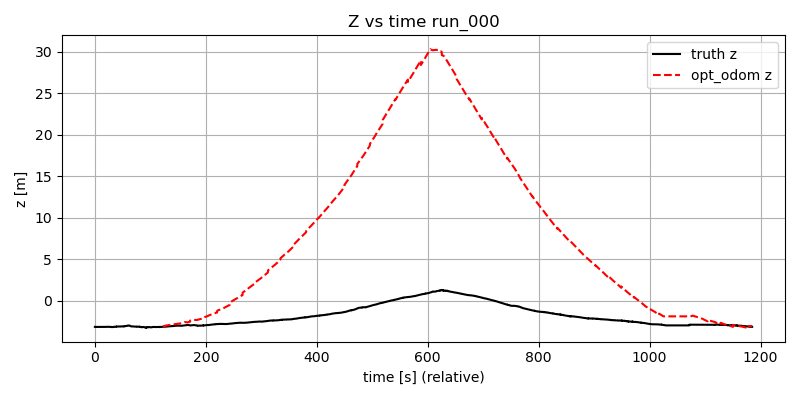
\includegraphics[width=\textwidth]{3-SLAM/3-results/figures/ds3_z.png}
        \caption{Baseline | Dataset 3}
    \end{subfigure}
    \hfill
    \begin{subfigure}[b]{0.48\textwidth}
        \centering
        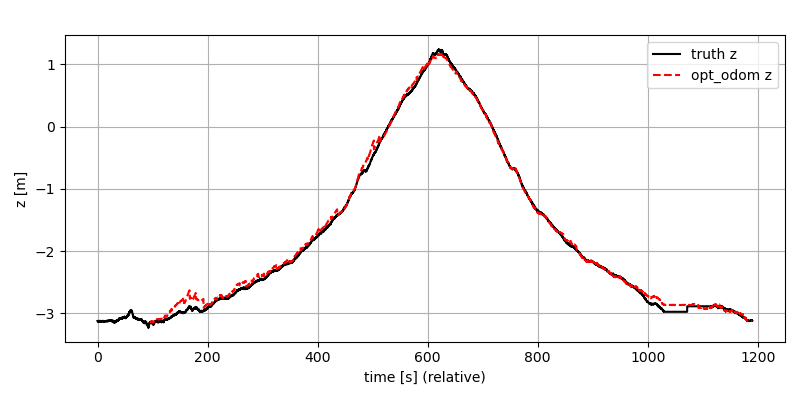
\includegraphics[width=\textwidth]{3-SLAM/3-results/figures/pds3_z.png}
        \caption{GLIM-GNSS | Dataset 3}
    \end{subfigure}

    \vspace{1em}

    % --- ROW 5 ---
    \begin{subfigure}[b]{0.48\textwidth}
        \centering
        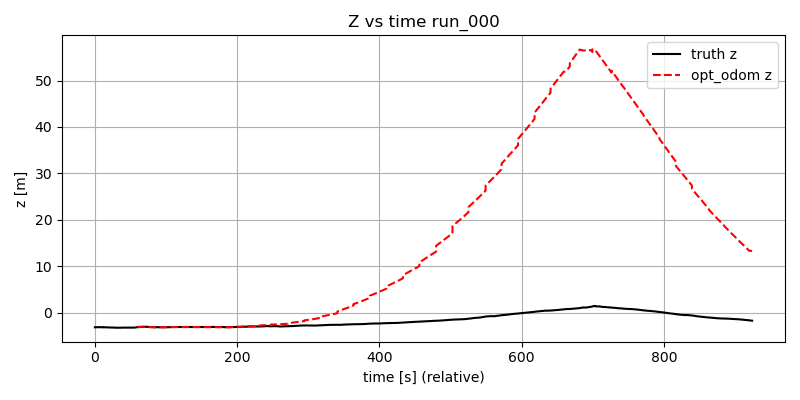
\includegraphics[width=\textwidth]{3-SLAM/3-results/figures/ds4_z.png}
        \caption{Baseline | Dataset 4}
        \label{fig:ds4_z_baseline}
    \end{subfigure}
    \hfill
    \begin{subfigure}[b]{0.48\textwidth}
        \centering
        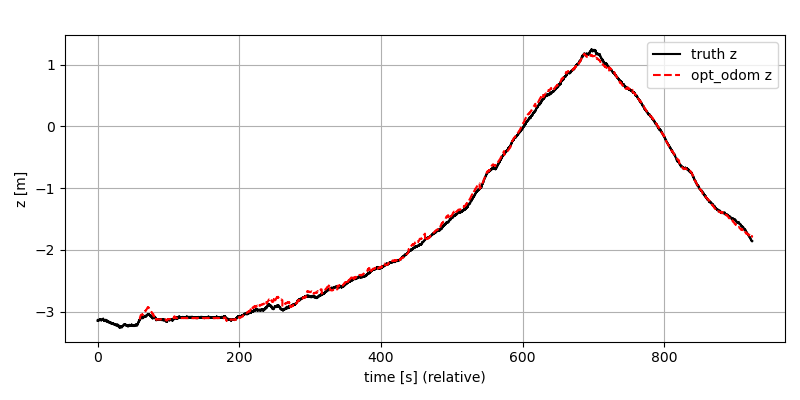
\includegraphics[width=\textwidth]{3-SLAM/3-results/figures/pds4_z.png}
        \caption{GLIM-GNSS | Dataset 4}
    \end{subfigure}

    \caption{Trajectories in Z plane from baseline GLIM and GLIM-GNSS.}
    \label{fig:large_grid_z}
\end{figure}

% ===== Precise Alignment: LiDAR Heatmap =====
\section{Precise Alignment Supplementary Figures}
\label{app:pa-supplementary-figures}

\begin{figure}[htbp]
  \centering
  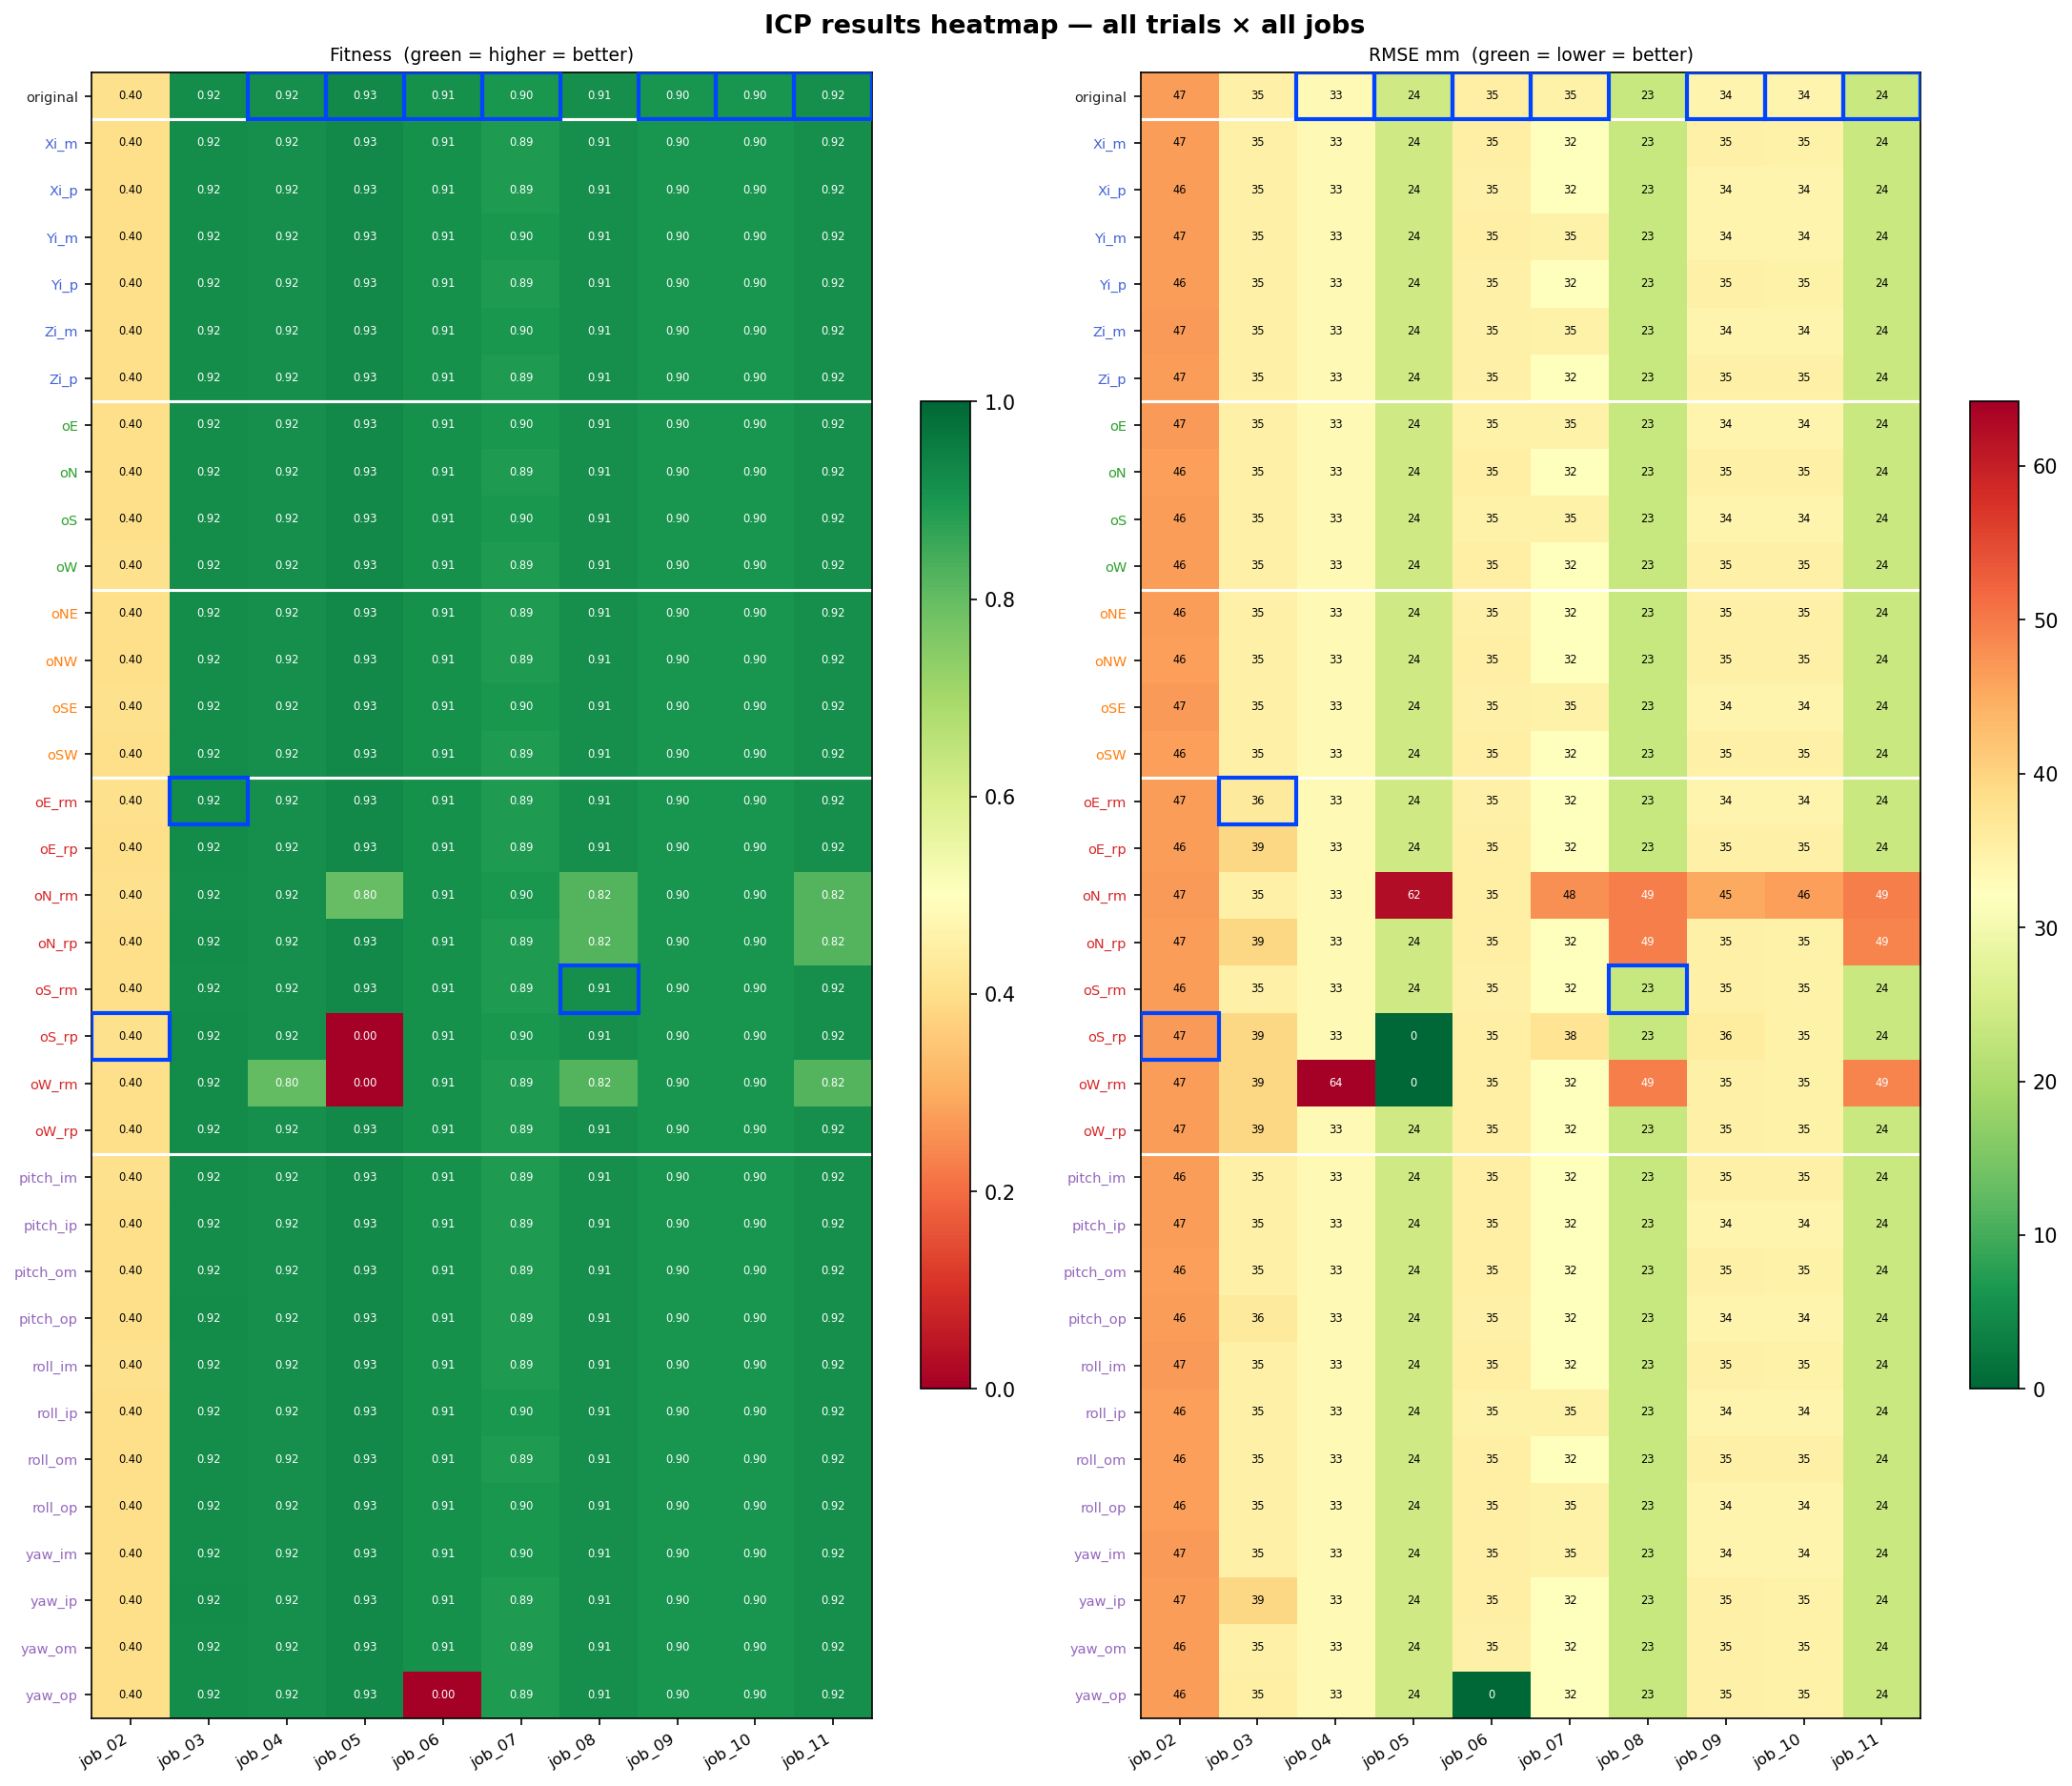
\includegraphics[width=\linewidth]{4-precise-alignment/4-results/figures/lidar_icp_heatmap}
  \caption{ICP fitness heatmap across all 315 LiDAR hypotheses. Each row corresponds to one condition (ordered by distance); each column to one perturbation hypothesis. Colour intensity indicates fitness score. The D110A0 row was excluded from analysis as it exceeded the stereo pipeline's depth clipping threshold.}
  \label{fig:pa-lidar-heatmap}
\end{figure}

\begin{figure}[htbp]
  \centering
  \begin{subfigure}[b]{0.32\linewidth}
    \centering
    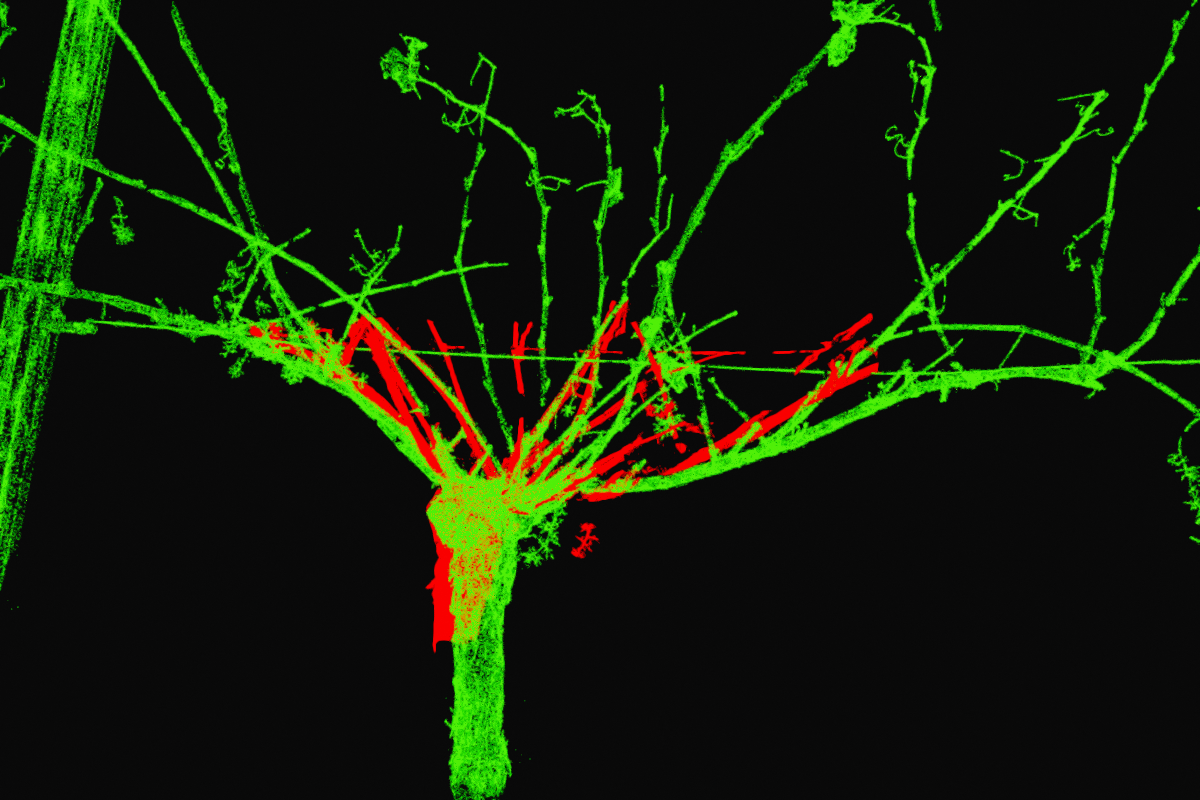
\includegraphics[width=\linewidth]{4-precise-alignment/4-results/figures/stereo_D40Am15_5b_icp_final_side}
    \caption{D40A$-$15}
  \end{subfigure}
  \hfill
  \begin{subfigure}[b]{0.32\linewidth}
    \centering
    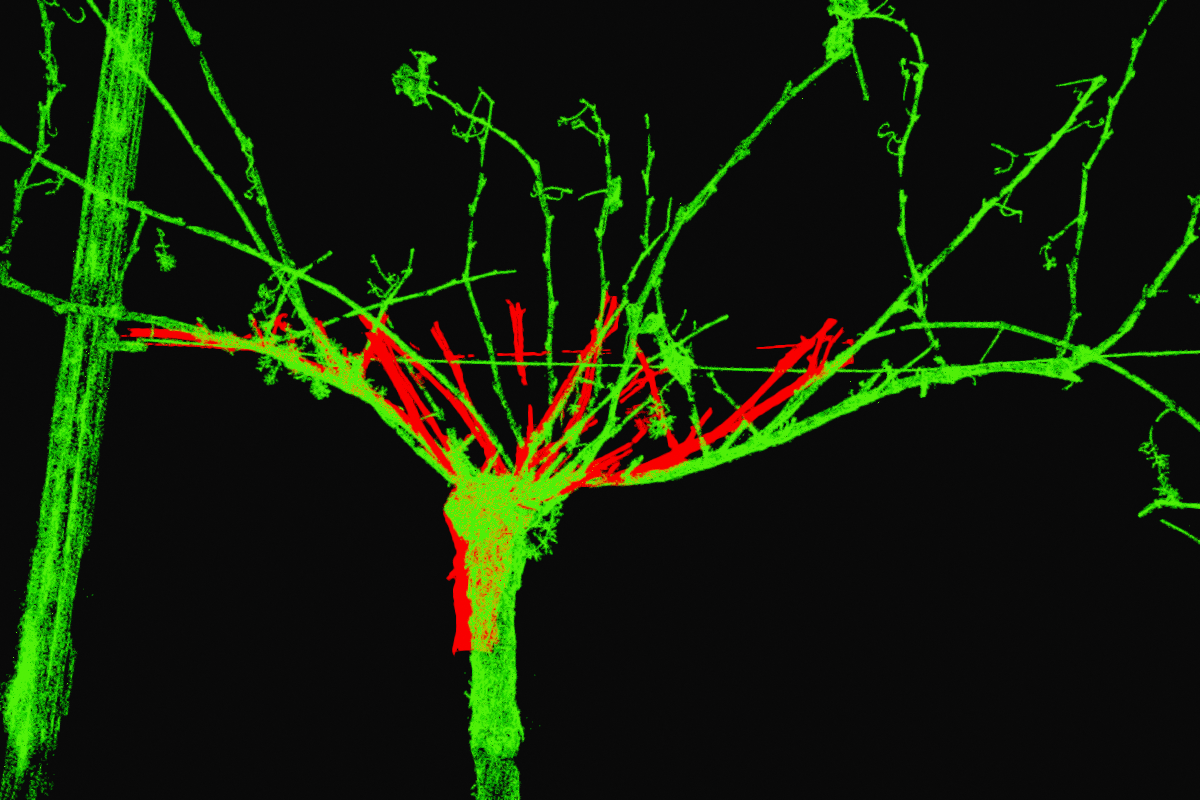
\includegraphics[width=\linewidth]{4-precise-alignment/4-results/figures/stereo_D40A0_5b_icp_final_side}
    \caption{D40A0}
  \end{subfigure}
  \hfill
  \begin{subfigure}[b]{0.32\linewidth}
    \centering
    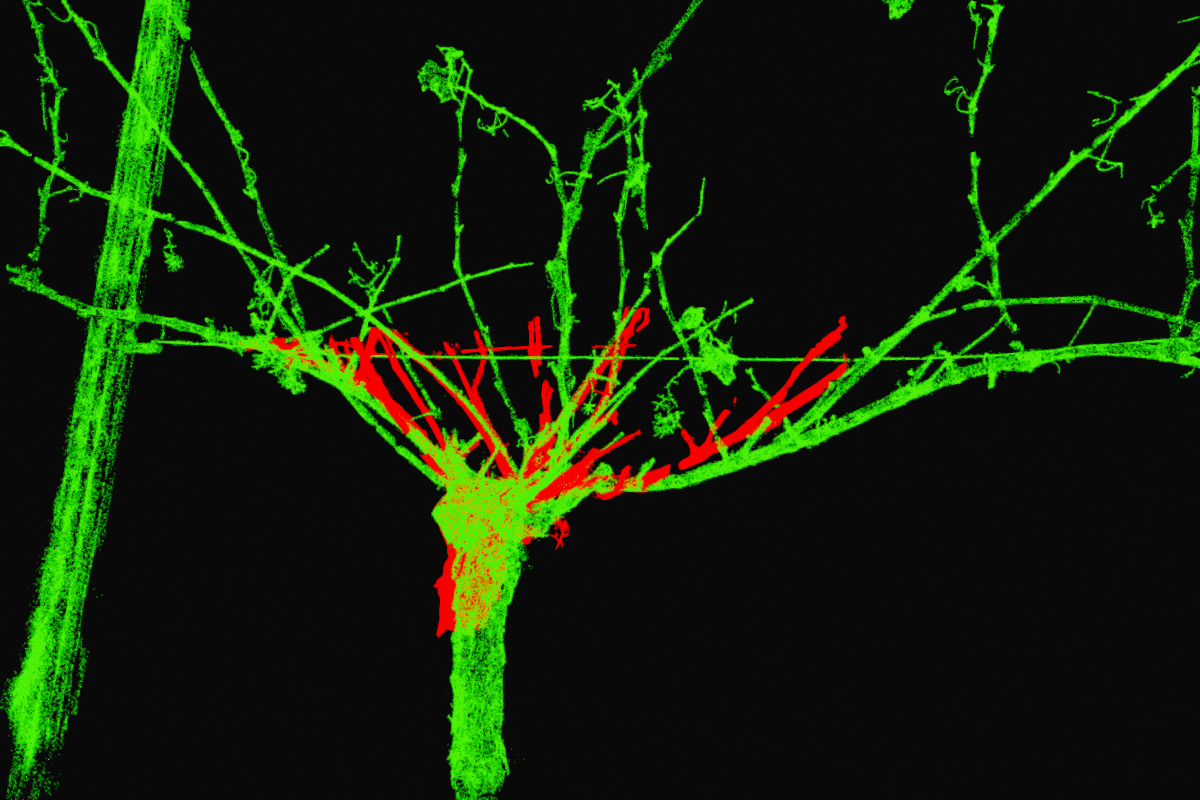
\includegraphics[width=\linewidth]{4-precise-alignment/4-results/figures/stereo_D60Am15_5b_icp_final_side}
    \caption{D60A$-$15}
  \end{subfigure}

  \vspace{0.5em}

  \begin{subfigure}[b]{0.32\linewidth}
    \centering
    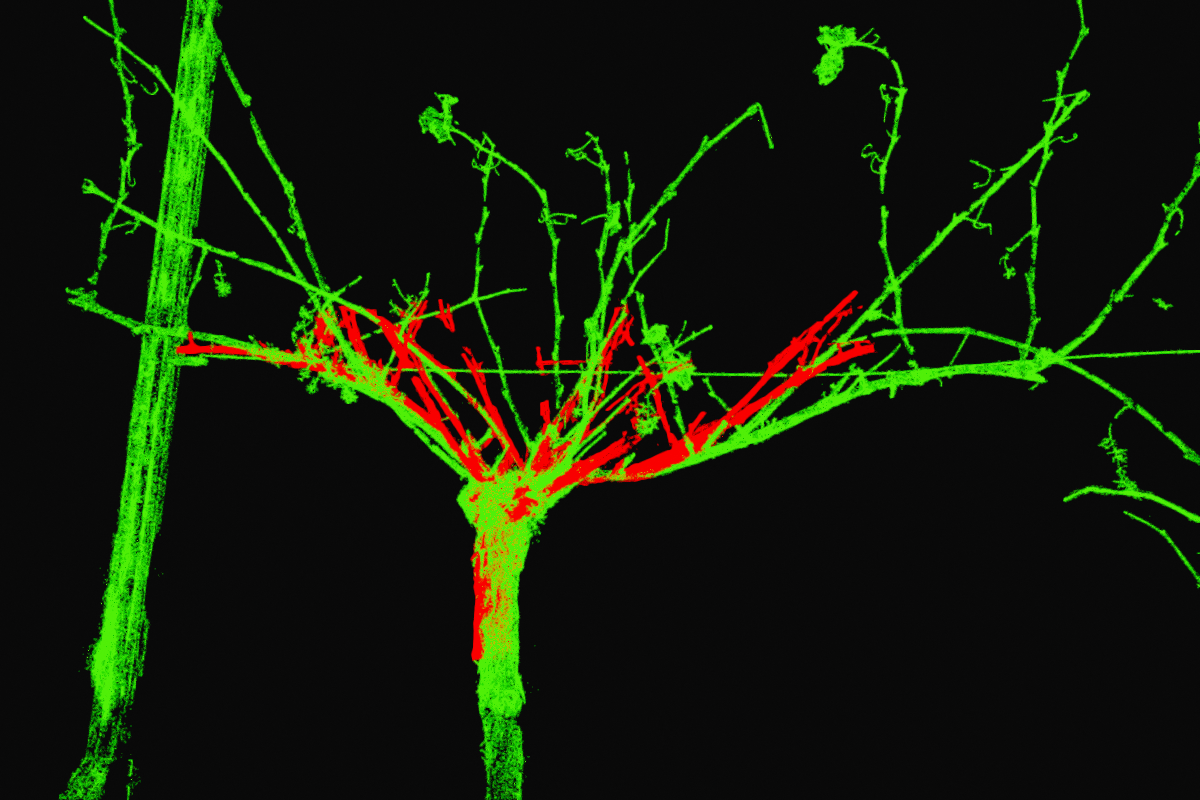
\includegraphics[width=\linewidth]{4-precise-alignment/4-results/figures/stereo_D60A0_5b_icp_final_side}
    \caption{D60A0}
  \end{subfigure}
  \hfill
  \begin{subfigure}[b]{0.32\linewidth}
    \centering
    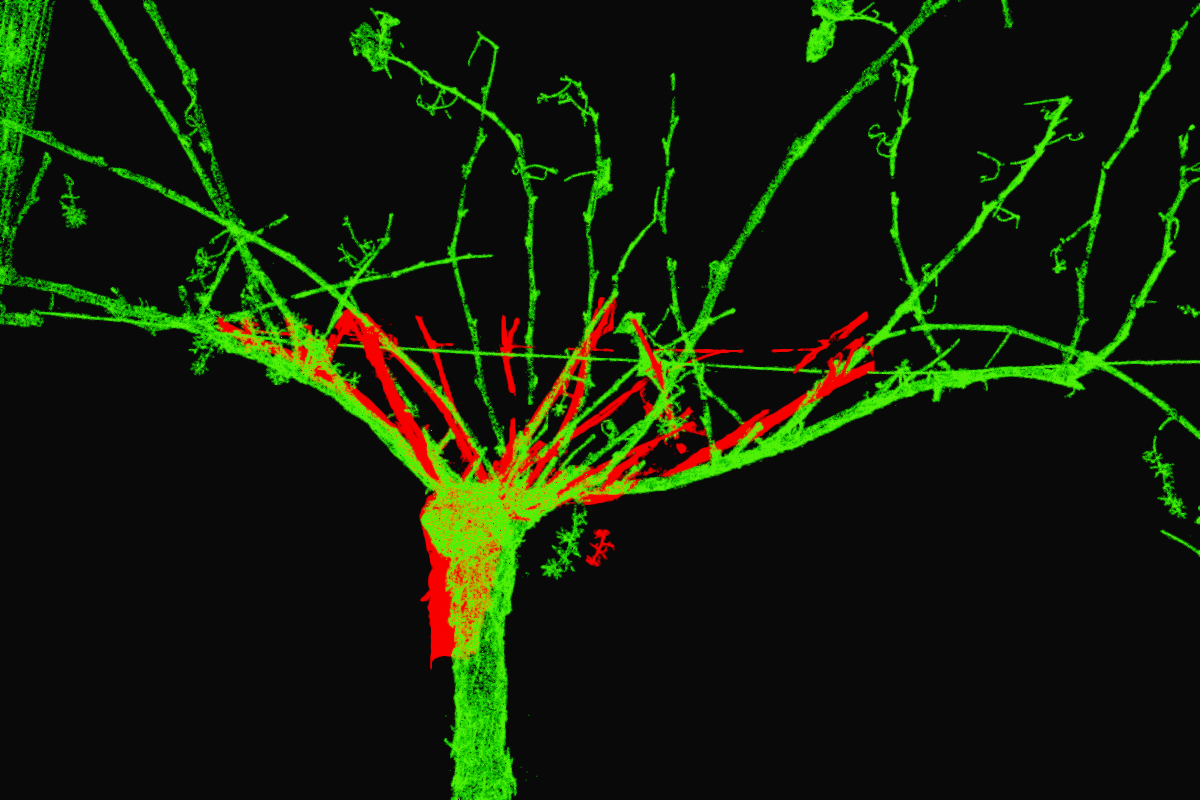
\includegraphics[width=\linewidth]{4-precise-alignment/4-results/figures/stereo_D60Ap15_5b_icp_final_side}
    \caption{D60A$+$15}
  \end{subfigure}
  \hfill
  \begin{subfigure}[b]{0.32\linewidth}
    \centering
    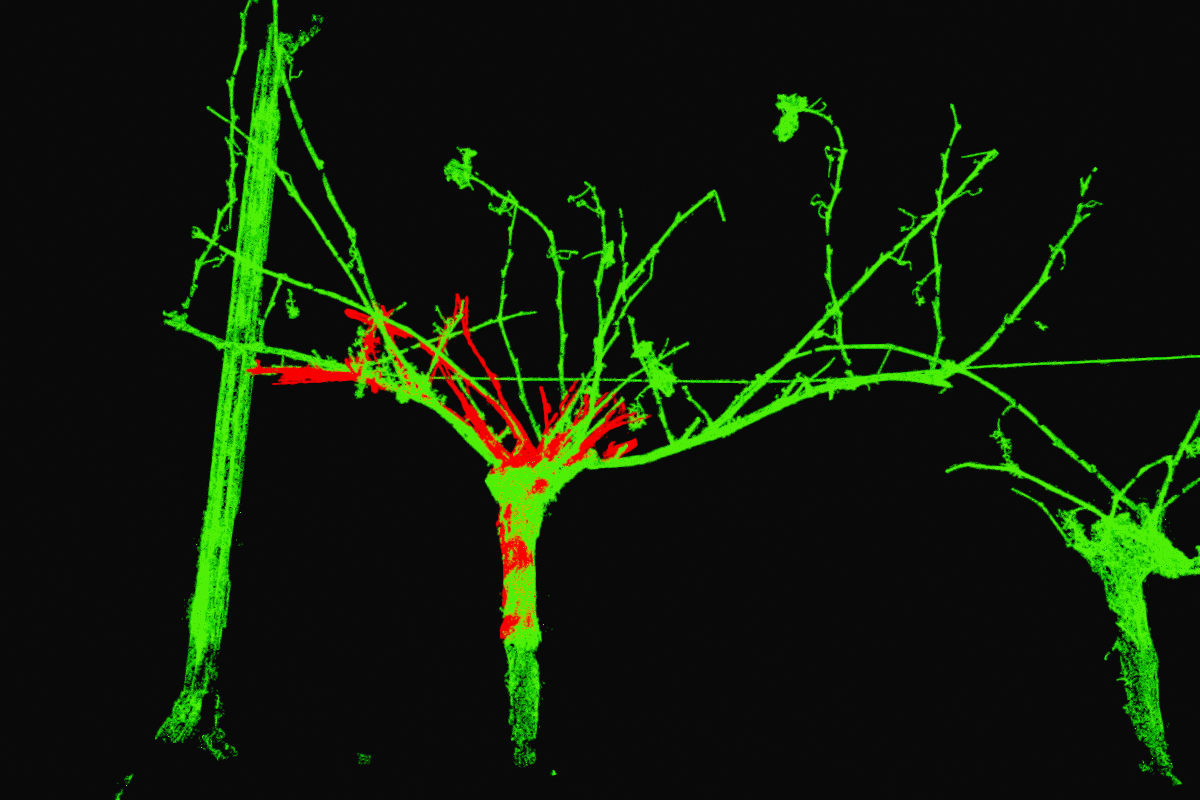
\includegraphics[width=\linewidth]{4-precise-alignment/4-results/figures/stereo_D80A0_5b_icp_final_side}
    \caption{D80A0}
  \end{subfigure}

  \vspace{0.5em}

  \begin{subfigure}[b]{0.32\linewidth}
    \centering
    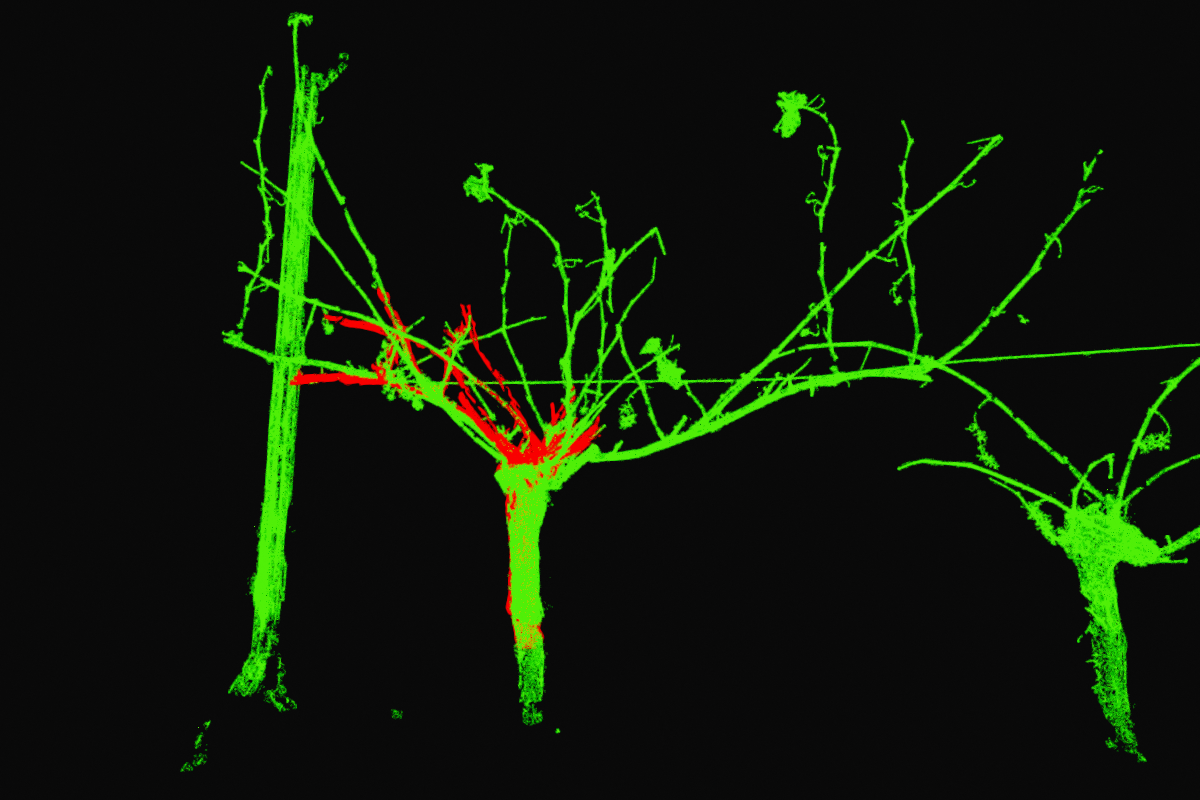
\includegraphics[width=\linewidth]{4-precise-alignment/4-results/figures/stereo_D80Ap15_5b_icp_final_side}
    \caption{D80A$+$15}
  \end{subfigure}
  \caption{Final stereo ICP alignment (vine-face view) for all seven converging conditions. Green: 3DGS reference cloud; red: registered stereo source cloud.}
  \label{fig:pa-stereo-converged-overlay}
\end{figure}

\end{document}
